% Customizable fields and text areas start with % >> below.
% Lines starting with the comment character (%) are normally removed before release outside the collaboration, but not those comments ending lines

% svn info. These are modified by svn at checkout time.
% The last version of these macros found before the maketitle will be the one on the front page,
% so only the main file is tracked.
% Do not edit by hand!
\RCS$Revision: 306273 $
\RCS$HeadURL: svn+ssh://svn.cern.ch/reps/tdr2/notes/AN-15-109/trunk/AN-15-109.tex $
\RCS$Id: AN-15-109.tex 306273 2015-10-21 03:17:11Z haweber $
%%%%%%%%%%%%% local definitions %%%%%%%%%%%%%%%%%%%%%
% This allows for switching between one column and two column (cms@external) layouts
% The widths should  be modified for your particular figures. You'll need additional copies if you have more than one standard figure size.
\newcommand{\MTtW}{\ensuremath{M_{\mathrm{T2}}^{\mathrm{W}}}\xspace}
\newcommand{\MTt}{\ensuremath{M_{\mathrm{T2}}}\xspace}
\newcommand{\MT}{\ensuremath{M_{\mathrm{T}}}\xspace}
\newcommand{\NJ}{\ensuremath{N_\mathrm{j}}\xspace}
\newcommand{\NB}{\ensuremath{N_\PQb}\xspace}
\newcommand{\dz}{\ensuremath{d_\mathrm{z}}\xspace}
\newcommand{\minDPhi}{\ensuremath{\min\Delta\phi}\xspace}
\newcommand{\minDPhiMETjet}{\ensuremath{\min\Delta\phi(j_{1,2},\MET)}\xspace}
\newcommand{\wjets}{\PW(\ensuremath{\ell\nu})+jets\xspace}
\newcommand{\zinv}{\Z(\ensuremath{\nu\PAGn})+jets\xspace}
\newcommand{\zlljets}{\Z(\ensuremath{\ell^{+}\ell^{-}})+jets\xspace}
\newcommand{\zll}{Z(\ensuremath{\ell^{+}\ell^{-}})\xspace}
\newcommand{\gjets}{\ensuremath{\gamma}+jets\xspace}
\newcommand{\ZG}{\ensuremath{\Z(\nu\PAGn)/\gamma}\xspace}
\newcommand{\ttjets}{\ttbar+jets\xspace}
\newcommand{\mb}{\ensuremath{m_{\PQb}}\xspace}
\newcommand{\mbb}{\ensuremath{M_{\PQb\PQb}}\xspace}
\newcommand{\mlsp}{\ensuremath{m_{\PSGczDo}}\xspace}
\newcommand{\mneutTwo}{\ensuremath{m_{\PSGczDt}}\xspace}
\newcommand{\mcharg}{\ensuremath{m_{\PSGczDopm}}\xspace}
\newcommand{\mgluino}{\ensuremath{m_{\PSg}}\xspace}
\newcommand{\msq}{\ensuremath{m_{\PSQ}}\xspace}
\newcommand{\mstop}{\ensuremath{m_{\PSQt}}\xspace}
\newcommand{\mtop}{\ensuremath{m_{\PQt}}\xspace}
\providecommand{\PSGczDopm}{\ensuremath{\widetilde{\chi}^{\pm}_{1}}\xspace}
\providecommand{\NA}{\text{---}\xspace}
\providecommand{\CLs}{\ensuremath{\textrm{CL}_{\textrm{s}}}\xspace}
\providecommand{\CLsb}{\ensuremath{\textrm{CL}_{\textrm{s+b}}}\xspace}
\providecommand{\CLb}{\ensuremath{\textrm{CL}_{\textrm{b}}}\xspace}
\providecommand{\SOFTSUSY} {{\textsc{softsusy}}\xspace}
\providecommand{\SDECAY} {{\textsc{sdecay}}\xspace}
\providecommand{\Prospino} {{\textsc{Prospino}}\xspace}
\providecommand{\FastJet} {{\textsc{FastJet}}\xspace}

\newlength\cmsFigWidth
\ifthenelse{\boolean{cms@external}}{\setlength\cmsFigWidth{0.85\columnwidth}}{\setlength\cmsFigWidth{0.4\textwidth}}
\ifthenelse{\boolean{cms@external}}{\providecommand{\cmsLeft}{top\xspace}}{\providecommand{\cmsLeft}{left\xspace}}
\ifthenelse{\boolean{cms@external}}{\providecommand{\cmsRight}{bottom\xspace}}{\providecommand{\cmsRight}{right\xspace}}
%%%%%%%%%%%%%%%  Title page %%%%%%%%%%%%%%%%%%%%%%%%
\cmsNoteHeader{AN-15-109} % This is over-written in the CMS environment: useful as preprint no. for export versions
% >> Title: please make sure that the non-TeX equivalent is in PDFTitle below
\title{Search for Direct Top Squark Pair Production in the Single Lepton Channel at 13 TeV}

% >> Authors
%Author is always "The CMS Collaboration" for PAS and papers, so author, etc, below will be ignored in those cases
%For multiple affiliations, create an address entry for the combination
%To mark authors as primary, use the \author* form
\address[fnal]{Fermilab}
\address[ucsb]{UCSB}
\address[ucsd]{UCSD}
\author[fnal]{L. Bauerdick} \author[fnal]{K. Burkett}  \author[fnal]{O. Gutsche}  \author[fnal]{S. Jindariani}  \author[fnal]{J. Linacre}  \author[fnal]{M. Liu}  \author[fnal]{R. Lopes de Sa}  \author[fnal]{H. Weber} 
\author[ucsb]{N. Amin} \author[ucsb]{C. Campagnari} \author[ucsb]{A. George} \author[ucsb]{F. Golf} \author[ucsb]{J. Gran} \author[ucsb]{I. Suarez} 
\author[ucsd]{G. Cerati} \author[ucsd]{I. Dyckes} \author[ucsd]{M. Derdzinski} \author[ucsd]{D. Klein} \author[ucsd]{I. MacNeill} \author[ucsd]{D. Olivito} \author[ucsd]{G. Zevi Della Porta} \author[ucsd]{C. Welke} \author[ucsd]{J. Wood} \author[ucsd]{F. W\"urthwein} \author[ucsd]{A. Yagil} 


% >> Date
% The date is in yyyy/mm/dd format. Today has been
% redefined to match, but if the date needs to be fixed, please write it in this fashion.
% For papers and PAS, \today is taken as the date the head file (this one) was last modified according to svn: see the RCS Id string above.
% For the final version it is best to "touch" the head file to make sure it has the latest date.
\date{\today}

% >> Abstract
% Abstract processing:
% 1. **DO NOT use \include or \input** to include the abstract: our abstract extractor will not search through other files than this one.
% 2. **DO NOT use %**                  to comment out sections of the abstract: the extractor will still grab those lines (and they won't be comments any longer!).
% 3. For PASs: **DO NOT use tex macros**         in the abstract: CDS MathJax processor used on the abstract doesn't understand them _and_ will only look within $$. The abstracts for papers are hand formatted so macros are okay.
\abstract{
%   This is an example of a \textit{CMS Note} written in \LaTeX
%    using the \emph{cms-tdr} document class and processed using the
%    same \texttt{tdr} perl script used in generating the CMS Physics TDRs.
%    Instructions for producing CMS Notes and Internal Notes are given.
This is a first write up of FNAL/UCSB/UCSD effort for scalar top quark partner search in final states with one electron or muon for 13\TeV.
}

% >> PDF Metadata
% Do not comment out the following hypersetup lines (metadata). They will disappear in NODRAFT mode and are needed by CDS.
% Also: make sure that the values of the metadata items are sensible and are in plain text:
% (1) no TeX! -- for \sqrt{s} use sqrt(s) -- this will show with extra quote marks in the draft version but is okay).
% (2) no %.
% (3) No curly braces {}.
\hypersetup{%
pdfauthor={F. Golf, D. Klein, , M. Liu, I. Suarez, H. Weber, J. Wood, F. Wuerthwein},%
pdftitle={Search for Direct Top Squark Pair Production in the Single Lepton Channel at 13 TeV},%
pdfsubject={CMS},%
pdfkeywords={CMS, physics, software, computing}}

\maketitle %maketitle comes after all the front information has been supplied
% >> Text
%%%%%%%%%%%%%%%%%%%%%%%%%%%%%%%%  Begin text %%%%%%%%%%%%%%%%%%%%%%%%%%%%%
%% **DO NOT REMOVE THE BIBLIOGRAPHY** which is located before the appendix.
%% You can take the text between here and the bibiliography as an example which you should replace with the actual text of your document.
%% If you include other TeX files, be sure to use "\input{filename}" rather than "\input filename".
%% The latter works for you, but our parser looks for the braces and will break when uploading the document.
%%%%%%%%%%%%%%%


\section{Introduction}
\label{sec:Intro}

%%%%%%%%%%%%%%%%%%%%%%%%%%%%%%%%
\section{Detector and trigger}
\label{sec:CMS}

The central feature of the CMS apparatus is a superconducting solenoid of 
6\unit{m} internal diameter, providing a magnetic field of 3.8\unit{T}. 
Within the superconducting solenoid volume are a silicon pixel and strip tracker, 
a lead-tungstate crystal electromagnetic calorimeter, and a brass{\slash}scintillator 
hadron calorimeter, each composed of a barrel and two endcap sections. 
Muons are measured in gas-ionization detectors embedded in the steel flux-return 
yoke outside the solenoid. Extensive forward calorimetry complements the coverage 
provided by the barrel and endcap detectors. 
%-- old
%The central feature of the CMS apparatus is a superconducting solenoid,
%13\unit{m} in length and 6\unit{m} in diameter, 
%that provides an axial magnetic field of 3.8\unit{T}.
%The core of the solenoid is instrumented with various particle detection
%systems: a silicon pixel 
%and strip tracker, an electromagnetic calorimeter (ECAL), and a
%brass/scintillator hadron calorimeter 
%(HCAL).  
%
%The silicon pixel and strip tracker covers $|\eta|<2.5$, ECAL and HCAL cover 
%$|\eta|<3$, and a quartz-steel Cerenkov-radiation-based forward hadron calorimeter extends the
%coverage to $|\eta| \leq 5$. 
%
The detector is nearly hermetic, covering $0<\phi<2\pi$ in azimuth, and thus allows
the measurement of momentum balance in the plane transverse to the beam
direction.
%
The first level of the CMS trigger system, composed of custom hardware
processors, uses information from the calorimeters and muon detectors to
select the most interesting events in a fixed time interval of less than
4~$\mu$s. The high level trigger processor farm further decreases the event
rate, from around 100\unit{kHz} to around 300\unit{Hz}, before data storage.
%The first level of the CMS trigger system, composed of custom hardware %Marcela's
%processors, uses information from the calorimeters and muon detectors to
%select the most interesting events. The High Level Trigger (HLT) utilizes a
%processor farm to further decrease the event rate.
%
A more detailed description of the CMS detector, together with a definition of the 
coordinate system used and the relevant kinematic variables, 
can be found in Ref.~\cite{Chatrchyan:2008aa}. 


%%%%%%%%%%%%%%%%%%%%%%%%%%%%%%%%


\section{Search strategy}
\label{sec:strategy}

The present section provides a brief overview of the dominant backgrounds, how they are suppressed,
and how the remaining background is estimated.

There are three types of backgrounds:
\begin{itemize}
\item Single lepton background
\item Lost lepton background
\item Background from $Z\to\nu\nu$
\end{itemize}

\subsection{Single Lepton background}

%This is the largest background for any search in the single isolated lepton plus jets plus \MET final state.
%It can be reduced dramatically with a combination of transverse mass and missing transverse momentum.
%
For any search in the single isolated lepton plus jets plus \MET final state, this background is the largest before any signal selection is applied. However, it can be reduced dramatically with a combination of transverse mass (\MT) and \MET.

Figure~\ref{fig:strategy:recoMT:W} shows the shape of the transverse mass distribution overlaid for \MET $\ge$ 50, 150, and 250\GeV
for W+jets Monte Carlo. It clearly shows the kinematic edge due to the W mass, and how this edge becomes more and more
dramatic as \MET is increased.

\begin{figure}
\subfigure[Reconstructed \MT distribution in reconstructed \PW($\ell\nu$)+jets events. The \PW~boson mass edge becomes steeper with increasing \MET requirement.]{
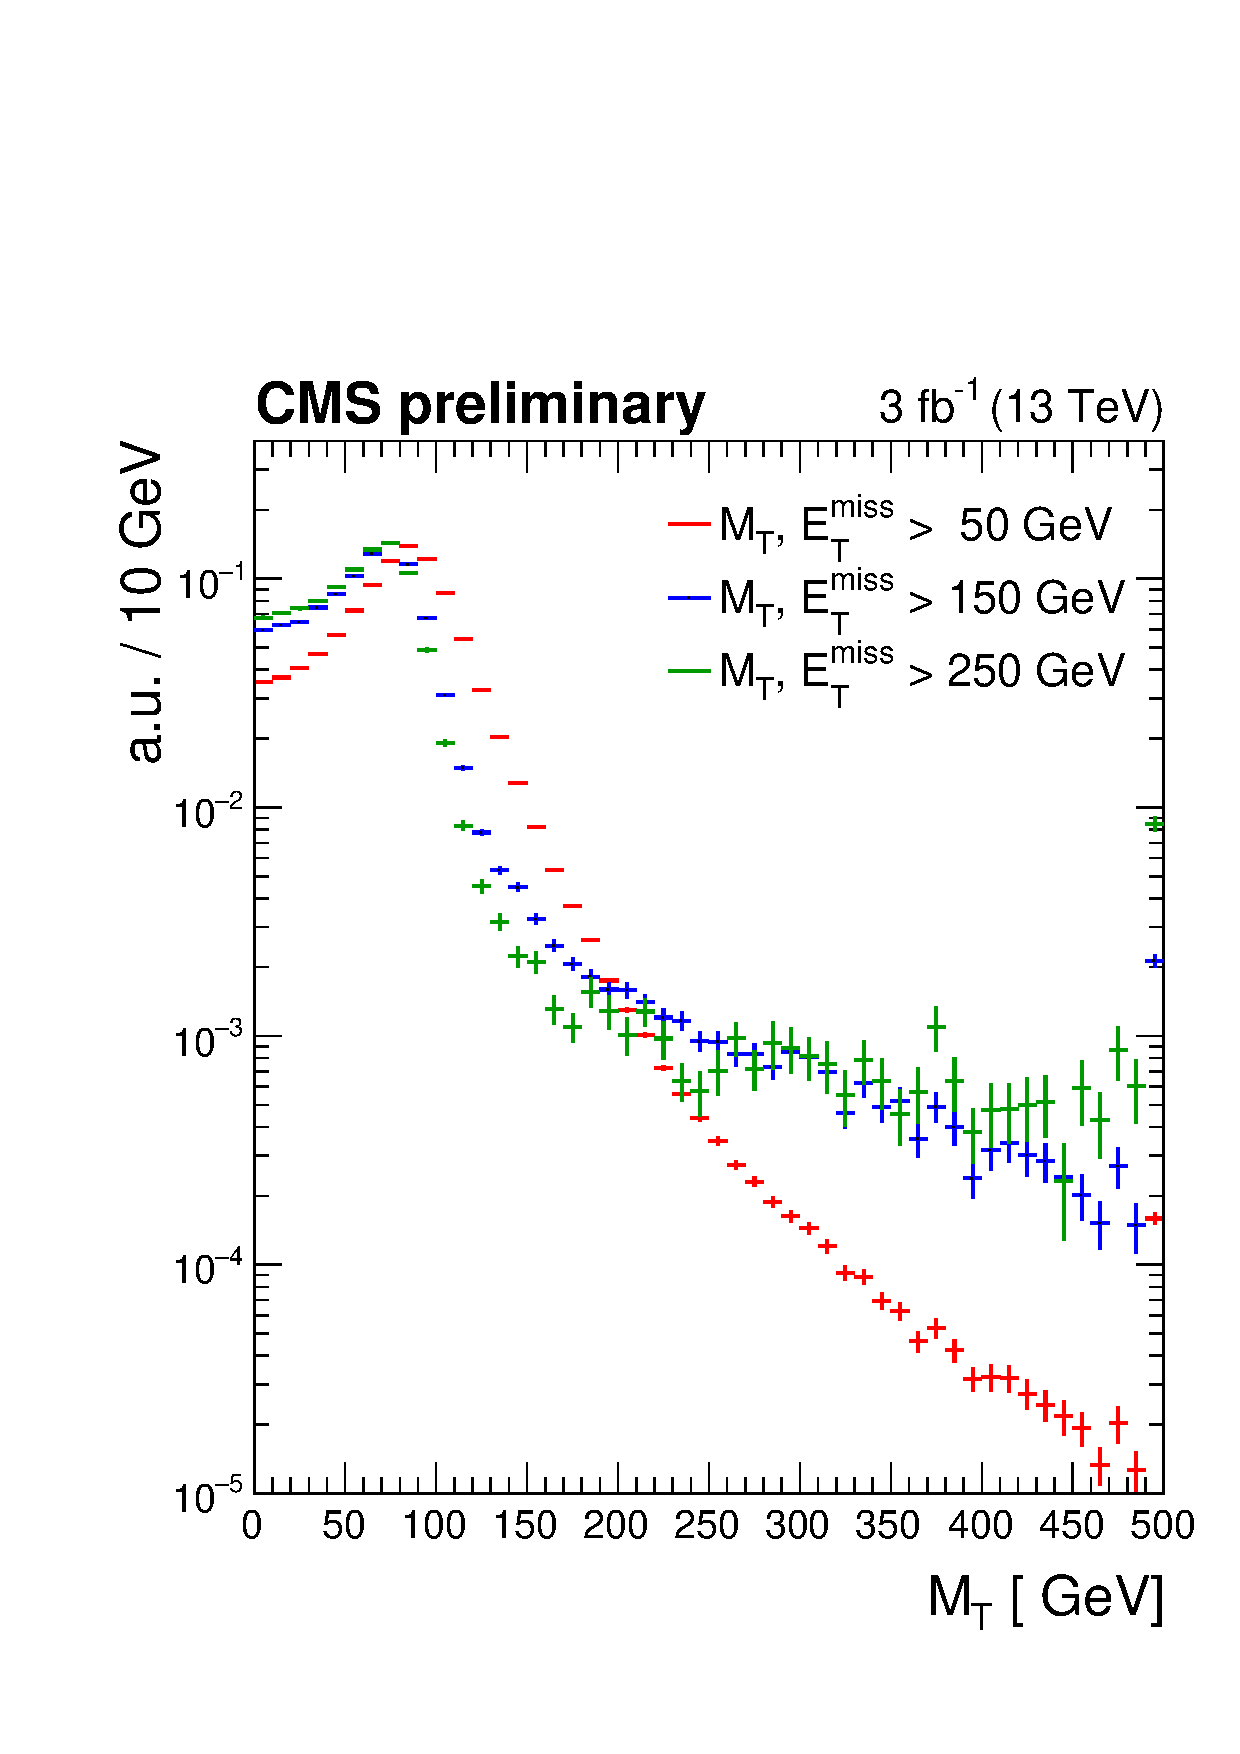
\includegraphics[width=0.3\textwidth]{Figures/Strat_MT_W.pdf}
\label{fig:strategy:recoMT:W}
}
\hspace{5pt}
\subfigure[Reconstructed and generator-truth \MT distribution in \PW($\ell\nu$)+jets and $\cPqt\cPaqt(\to1\ell)$+jets events.]{
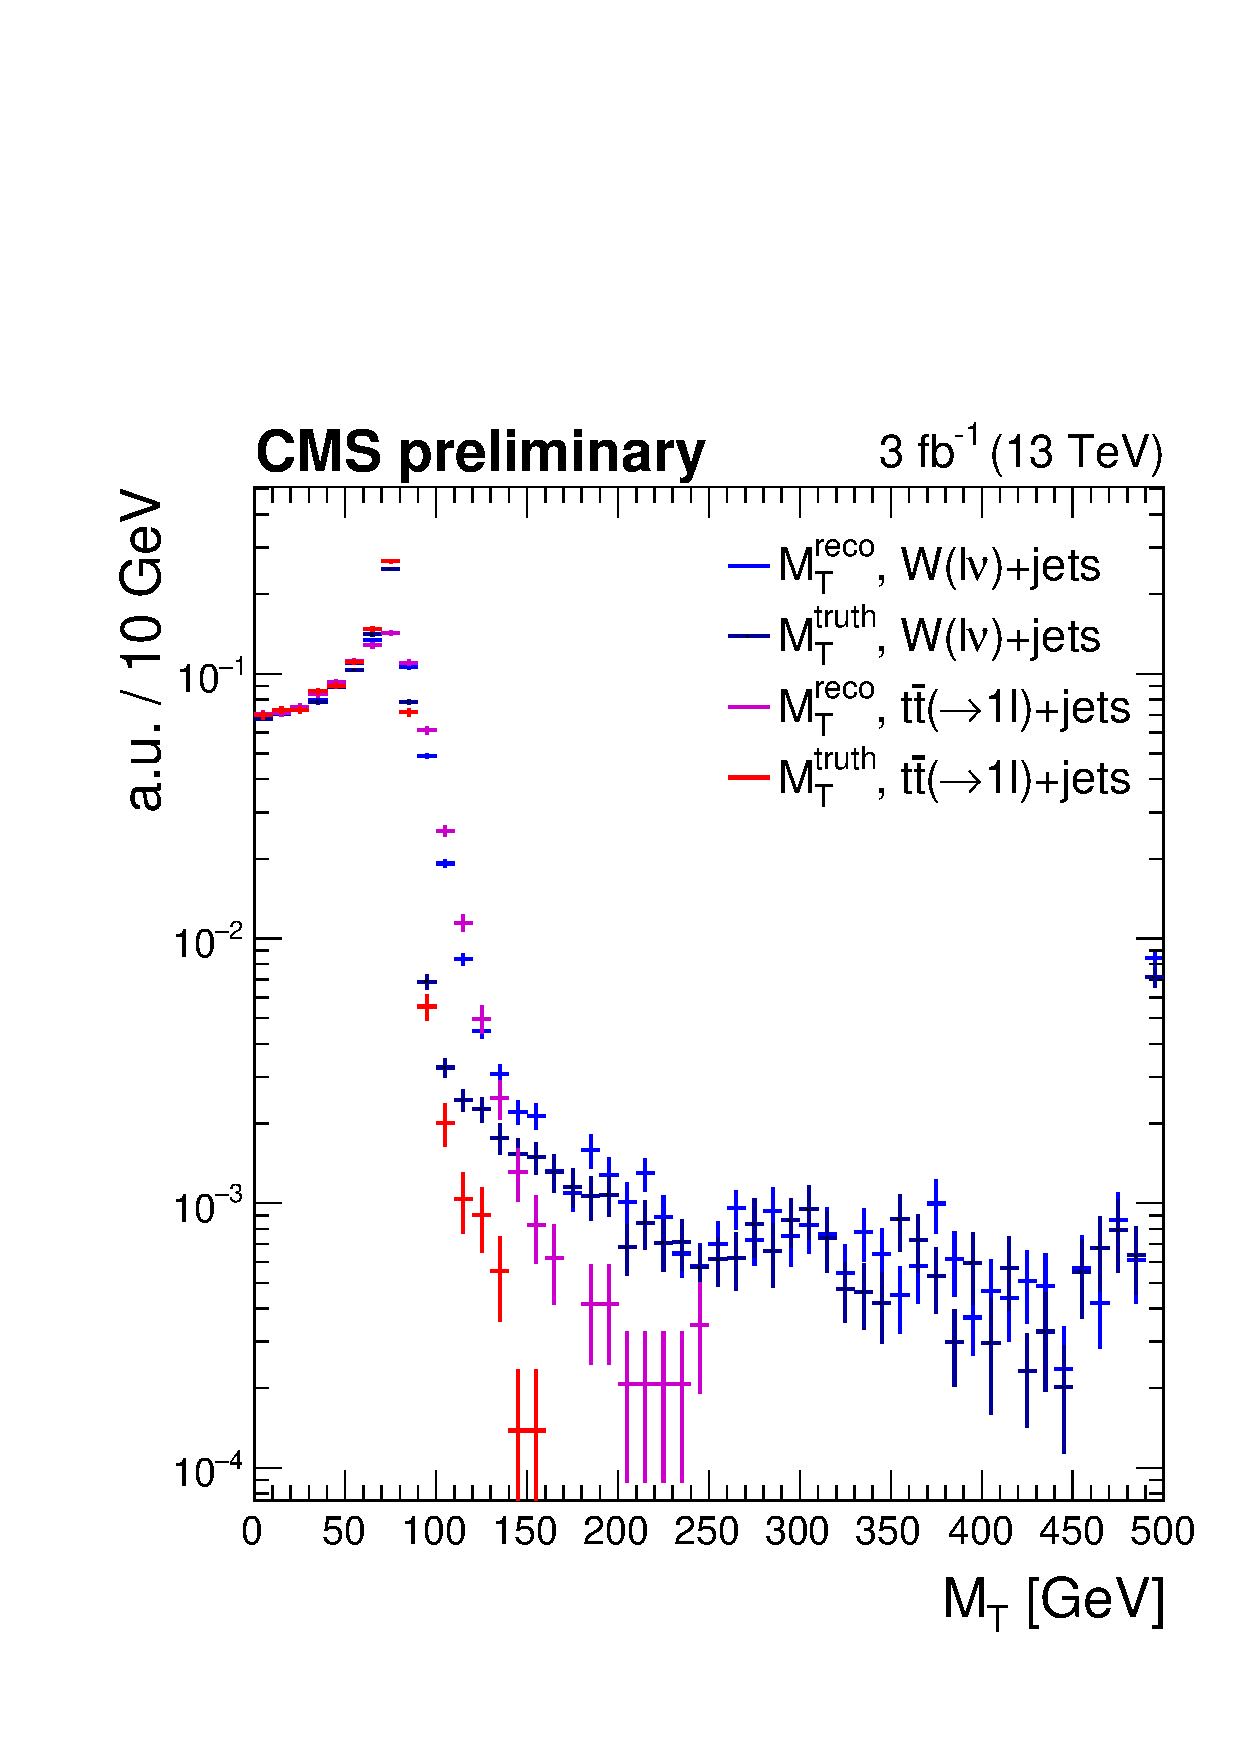
\includegraphics[width=0.3\textwidth]{Figures/Strat_MT_WTop.pdf}
\label{fig:strategy:recogenMT:Wttbar}
}
\hspace{5pt}
\subfigure[Generator-truth \MT distribution in reconstructed \PW($\ell\nu$)+jets events. The \PW~boson mass edge becomes steeper with increasing \MET requirement.]{
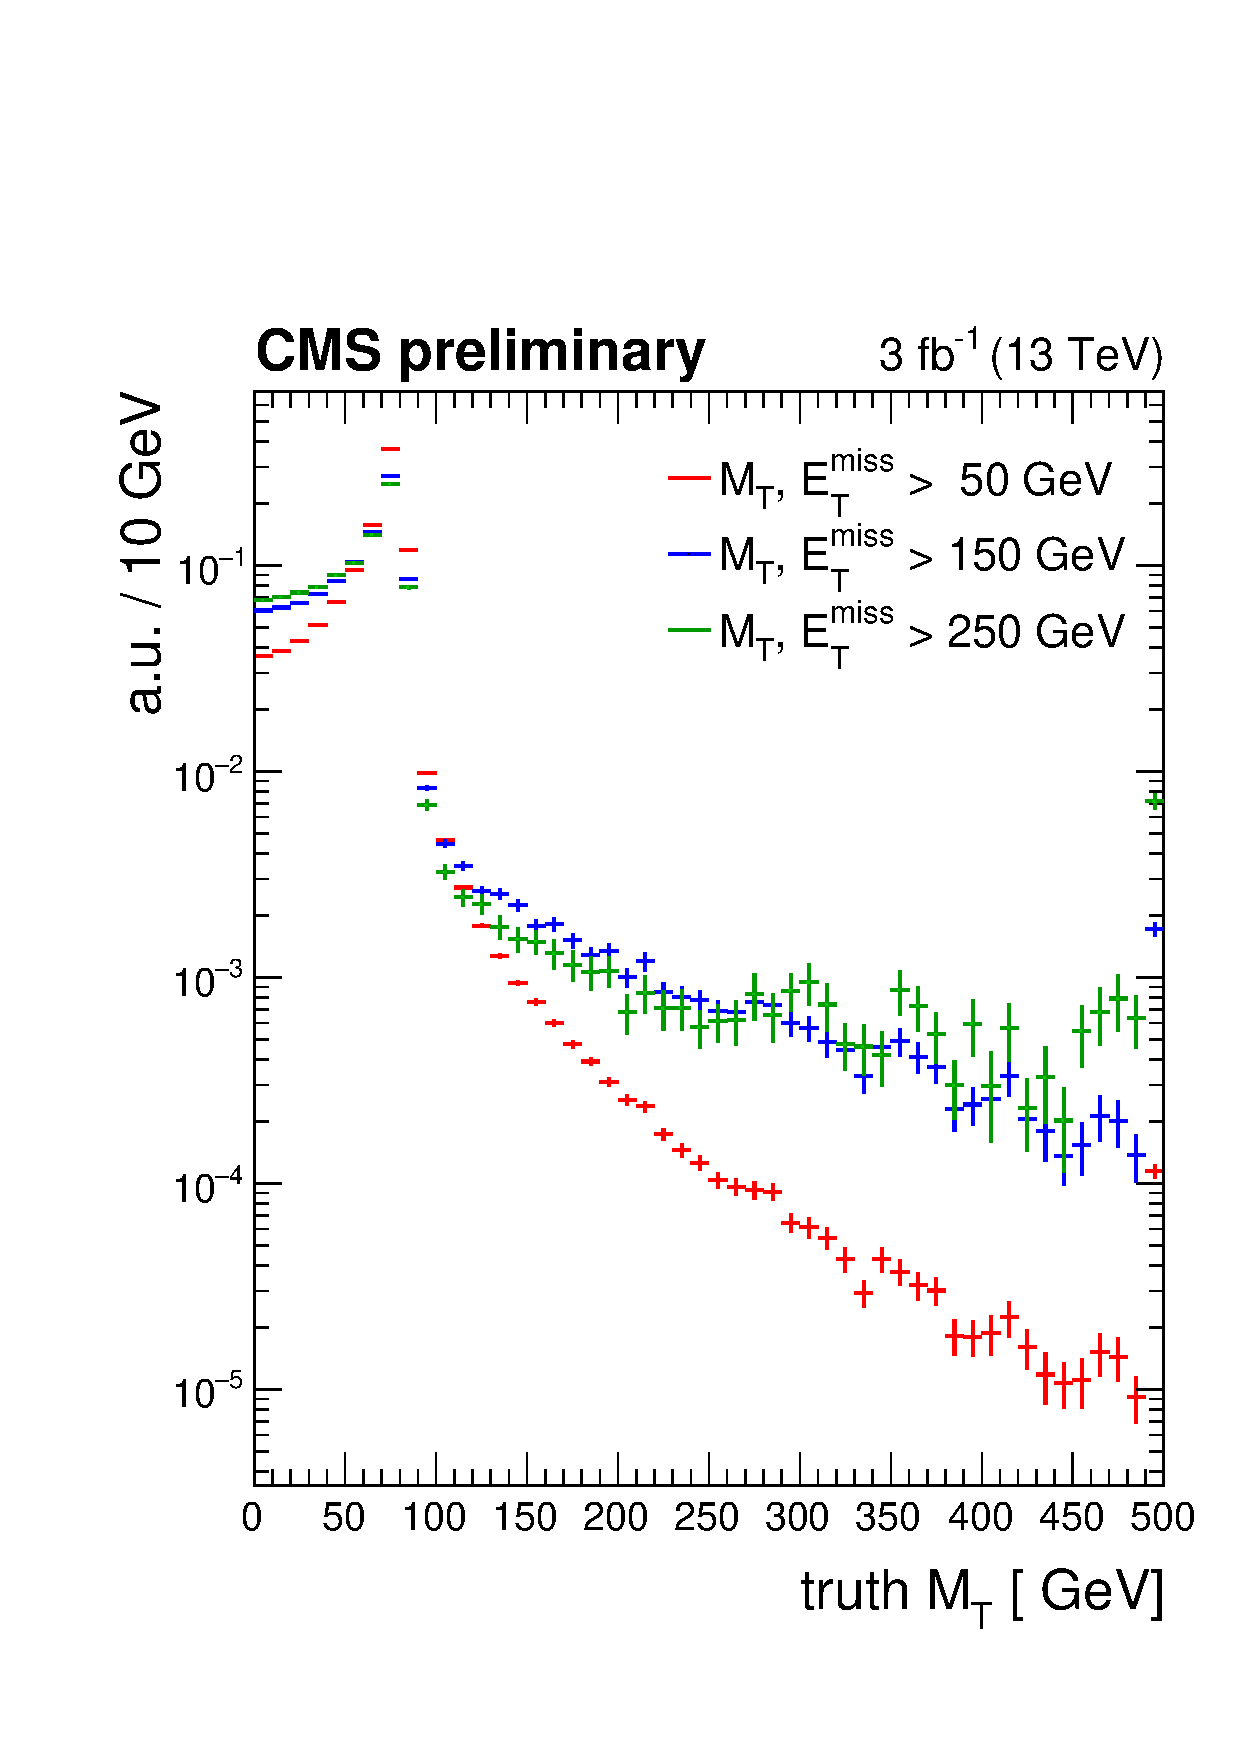
\includegraphics[width=0.3\textwidth]{Figures/Strat_MTtruth_W.pdf}
\label{fig:strategy:truthMT:W}
}
\caption{\label{fig:strategy:MT} \MT distributions.}
\end{figure}

Figure~\ref{fig:strategy:recogenMT:Wttbar} shows the shape of the transverse mass distribution for \MET $\ge$ 250\GeV, at least 2 jets and only one lepton 
at generator level, all with \pt $\ge$ 30\GeV. The Figure overlays generator and reco level transverse mass for W+jets and ttbar.
In both cases, we plot as generator level the transverse mass of the lepton neutrino pair. 
We see from this figure that the high transverse mass tail at generator level have dramatically different shapes for W+jets and ttbar. 
This is due to the fact that the top mass functions as a kinematic constraint on the W mass in ttbar, but no such constraint exists in W+jets.
As a result, the high transverse mass tail in ttbar 1-lepton events is dominated by \MET resolution effects, while for W+jets it is
largely driven by physics, i.e. the width of the W.

From these two simple figures, we learn that fundamentally, the 1-lepton background after \MT and \MET cuts is a complicated 
mix of relative production cross section of W+jets and ttbar, as well as \MET resolution effects. 
In practice, we picked our baseline cuts \MET$\ge$250\GeV and \MT$\ge$ 150\GeV such that 
the Monte Carlo predicts the 1-lepton ttbar background to be negligible in all our signal regions compared to W+jets.
This simplifies the analysis dramatically, and makes us only mildly dependent on systematic errors in the \MET resolution and/or
relative cross sections of ttbar and W+jets.

We then use zero b-tag control regions to normalize the W jets background in data. 
The details of these regions is a trade-off between statistics and ``extrapolation lever arm''.
A larger lever arm means better statistics in the control region but larger systematics due to the larger extrapolation.
For this analysis, we chose to extrapolate only in two variables, b-tagging and \MET for the W jets background.

In addition, we show via a combination of data and MC that 1-lepton ttbar background is indeed negligible, as expected,
and can thus be taken from Monte Carlo.

\subsection{Lost Lepton background}

The dominate background after \MET and \MT cuts as described above is ttbar with both W's decaying leptonically.
This background dominates even after carefully optimized 2nd lepton veto. We refer to this as "lost lepton" background
because typically the second lepton is either a hadronic tau that is not reconstructed, or an e,$\mu$ that is not isolated, or outside
\pt or $\eta$ acceptance of our lepton veto.

We estimate this background from dilepton control regions in data times transfer factors from Monte Carlo, and scale factors to account
for known differences in lepton efficiencies between data and Monte Carlo. 
The details are more complicated as this simplistic overview because we need to account for potential differences in 
gluon or quark radiation between data and Monte Carlo that affects lost hadronic tau and lost e or $\mu$ differently.

\subsection{Background from \texorpdfstring{$Z\to\nu\nu$}{Znunu}}

The dominant source of $Z\to\nu\nu$ in any of our signal regions is from ttbar + Z production where one of the two W's from top decay
decays leptonically. This background is not accounted for in either of the two previous estimation strategies in any way.
At some point in 2016, when we have plenty of data to measure both ttZ and tt$\gamma$ with $Z\to \ell\ell$ we might be able to define
a dedicated control region for ttZ. However, for the 2015 dataset, we will simply estimate ttZ from Monte Carlo, and use renormalization 
and factorization scale uncertainties evaluated as suggested by the CMS generator group as systematic uncertainty on this background.






\section{Triggers and datasets}
\label{sec:tridas}

\subsection{Triggers}
\label{sec:triggers}

As this search selects a single lepton final state, it is only natural to select events based on single lepton triggers.
However, the isolation definition at the online trigger level for both muons and electrons is different to the isolation definition we use offline in the analysis, leading to potential inefficiencies selection leptons. {\color{red} do we need a plot}
As our event selection will include $\MET>250\GeV$, see sec.~\ref{sec:obj_sel:signal_regions}, we can also use the \MET trigger.

Our final analysis trigger will be an OR of the lepton triggers and the MET triggers. They are listed on top of table~\ref{tab:tridas:triggers}.

In addition to those triggers, we additionally apply dilepton triggers to select the data in dilepton control region for the lost lepton background prediction, sec.~\ref{sec:bkgLL}.

Besides these triggers, we performed additional studies for \MET resolution using photon-triggered data.

For measuring signal efficiencies, we also will use \HT triggers.

All those auxiliary triggers are also listed in table~\ref{tab:tridas:triggers}.

\begin{table}[htb]
\centering
\caption{\label{tab:tridas:triggers} List of signal, control, and auxilary triggers. For auxiliary triggers, a wildcard * is used, meaning all threshold values available for that trigger type.}
\begin{tabular}{|l|c|}
\hline
type & name \\
\hline
\multirow{3}{*}{signal} & HLT\_Ele23\_WPLoose\_Gsf \\
 & HLT\_Iso(Tk)Mu20 \\%, HLT\_IsoTkMu20 \\
 & HLT\_PFMET170\_(\{Noise/JetId\}Cleaned) \\%, HLT\_PFMET170\_JetIdCleaned, HLT\_PFMET170 \\
 \hline
 \multirow{4}{*}{control} & HLT\_Mu17\_TrkIsoVVL\_Ele12\_CaloIdL\_TrackIdL\_IsoVL \\
   & HLT\_Mu8\_TrkIsoVVL\_Ele17\_CaloIdL\_TrackIdL\_IsoVL \\
   & HLT\_Ele23\_Ele12\_CaloIdL\_TrackIdL\_IsoVL\_DZ \\
   & HLT\_Mu17\_TrkIsoVVL\_(Tk)Mu8\_TrkIsoVVL\_DZ \\
\hline
\multirow{3}{*}{auxiliary} & HLT\_Photon*\_R9Id90\_HE10\_IsoM \\
  & HLT\_Photon165\_HE10 \\
  & HLT\_Photon175 \\
\hline
\multirow{2}{*}{auxiliary} & HLT\_PFHT* \\
 & HLT\_HT* \\
\hline
\end{tabular}
\end{table}

{\color{red} Add trigger efficiency here.}

\subsection{Simulation samples}
\label{sec:samples}

Table~\ref{tab:tridas:samples} contains the list of samples used in this analysis, together with their cross section values, which are either normalized to the best known cross section (usually NLO) or taken from MCM.

\begin{table}[htb]
\centering
\tiny
\caption{\label{tab:tridas:samples} List of simulation samples used, together with their cross-section $\sigma$.}
\setlength{\tabcolsep}{1pt}
\begin{tabular}{|l|c|c|}
\hline
 sample & main & $\sigma$ [pb] \\
 \hline
 /TT\_TuneCUETP8M1\_13TeV-powheg-pythia8/RunIISpring15MiniAODv2-74X\_mcRun2\_asymptotic\_v2(\_ext3)-v1/MINIAODSIM & $\times$ & 832 \\
 /TTJets\_SingleLeptFromT(bar)\_TuneCUETP8M1\_13TeV-madgraphMLM-pythia8/RunIISpring15MiniAODv2-74X\_mcRun2\_asymptotic\_v2(\_ext1)-v1/MINIAODSIM & --- & 183 \\
 /TTJets\_DiLept\_TuneCUETP8M1\_13TeV-madgraphMLM-pythia8/RunIISpring15MiniAODv2-74X\_mcRun2\_asymptotic\_v2(\_ext1)-v1/MINIAODSIM & --- & 87.3 \\
 \hline
/ST\_tW\_(anti)top\_5f\_inclusiveDecays\_13TeV-powheg-pythia8\_TuneCUETP8M1/RunIISpring15MiniAODv2-74X\_mcRun2\_asymptotic\_v2-v1/MINIAODSIM  & $\times$ & 35.6 \\
/ST\_t-channel\_(anti)top\_4f\_leptonDecays\_13TeV-powheg-pythia8\_TuneCUETP8M1/RunIISpring15MiniAODv2-74X\_mcRun2\_asymptotic\_v2-v1/MINIAODSIM & $\times$ & 44.1(26.2) \\
/ST\_s-channel\_4f\_leptonDecays\_13TeV-amcatnlo-pythia8\_TuneCUETP8M1/RunIISpring15MiniAODv2-74X\_mcRun2\_asymptotic\_v2-v1/MINIAODSIM & $\times$ & 3.7 \\
/tZq\_ll\_4f\_13TeV-amcatnlo-pythia8\_TuneCUETP8M1/RunIISpring15MiniAODv2-74X\_mcRun2\_asymptotic\_v2-v1/MINIAODSIM & $\times$ & 0.076 \\
/tZq\_nunu\_4f\_13TeV-amcatnlo-pythia8\_TuneCUETP8M1/RunIISpring15MiniAODv2-74X\_mcRun2\_asymptotic\_v2-v1/MINIAODSIM & $\times$ & 0.138 \\
\hline
/TTWJetsToLNu\_TuneCUETP8M1\_13TeV-amcatnloFXFX-madspin-pythia8/RunIISpring15MiniAODv2-74X\_mcRun2\_asymptotic\_v2-v1/MINIAODSIM  & $\times$ & 0.204 \\
/TTZToLLNuNu\_M-10\_TuneCUETP8M1\_13TeV-amcatnlo-pythia8/RunIISpring15MiniAODv2-74X\_mcRun2\_asymptotic\_v2-v2/MINIAODSIM & $\times$ & 0.253 \\
\hline
/WJetsToLNu\_HT-100To200\_TuneCUETP8M1\_13TeV-madgraphMLM-pythia8/RunIISpring15MiniAODv2-74X\_mcRun2\_asymptotic\_v2-v1/MINIAODSIM  & $\times$ & 1627 \\
 /WJetsToLNu\_HT-200To400\_TuneCUETP8M1\_13TeV-madgraphMLM-pythia8/RunIISpring15MiniAODv2-74X\_mcRun2\_asymptotic\_v2-v1/MINIAODSIM  & $\times$ & 435 \\
/WJetsToLNu\_HT-400To600\_TuneCUETP8M1\_13TeV-madgraphMLM-pythia8/RunIISpring15MiniAODv2-74X\_mcRun2\_asymptotic\_v2-v1/MINIAODSIM  & $\times$ &  59.2 \\
 /WJetsToLNu\_HT-600To800\_TuneCUETP8M1\_13TeV-madgraphMLM-pythia8/RunIISpring15MiniAODv2-74X\_mcRun2\_asymptotic\_v2-v1/MINIAODSIM & $\times$ & 14.6 \\
 /WJetsToLNu\_HT-800To1200\_TuneCUETP8M1\_13TeV-madgraphMLM-pythia8/RunIISpring15MiniAODv2-74X\_mcRun2\_asymptotic\_v2-v1/MINIAODSIM & $\times$ &  6.66 \\
  /WJetsToLNu\_HT-1200To2500\_TuneCUETP8M1\_13TeV-madgraphMLM-pythia8/RunIISpring15MiniAODv2-74X\_mcRun2\_asymptotic\_v2-v1/MINIAODSIM & $\times$ &  1.61 \\
   /WJetsToLNu\_HT-2500ToInf\_TuneCUETP8M1\_13TeV-madgraphMLM-pythia8/RunIISpring15MiniAODv2-74X\_mcRun2\_asymptotic\_v2-v1/MINIAODSIM  & $\times$ & 0.039 \\
\hline
/DYJetsToLL\_M-10to50\_TuneCUETP8M1\_13TeV-amcatnloFXFX-pythia8/RunIISpring15MiniAODv2-74X\_mcRun2\_asymptotic\_v2-v1/MINIAODSIM & --- & 20'657 \\
 /DYJetsToLL\_M-50\_TuneCUETP8M1\_13TeV-amcatnloFXFX-pythia8/RunIISpring15MiniAODv2-74X\_mcRun2\_asymptotic\_v2-v1/MINIAODSIM & --- & 6'025 \\
 \hline
  /WWTo2L2Nu\_13TeV-powheg/RunIISpring15MiniAODv2-74X\_mcRun2\_asymptotic\_v2-v1/MINIAODSIM  & $\times$ & 12.18 \\
 /WWToLNuQQ\_13TeV-powheg/RunIISpring15MiniAODv2-74X\_mcRun2\_asymptotic\_v2-v1/MINIAODSIM  & $\times$ & 50.0 \\
  /WZTo2L2Q\_13TeV\_amcatnloFXFX\_madspin\_pythia8/RunIISpring15MiniAODv2-74X\_mcRun2\_asymptotic\_v2-v1/MINIAODSIM & --- & 5.59 \\
  /WZTo1L1Nu2Q\_13TeV\_amcatnloFXFX\_madspin\_pythia8/RunIISpring15MiniAODv2-74X\_mcRun2\_asymptotic\_v2-v1/MINIAODSIM & $\times$ & 10.72 \\
   /WZTo1L3Nu\_13TeV\_amcatnloFXFX\_madspin\_pythia8/RunIISpring15MiniAODv2-74X\_mcRun2\_asymptotic\_v2-v1/MINIAODSIM & $\times$ & 3.05 \\
 /ZZTo2L2Nu\_13TeV\_powheg\_pythia8/RunIISpring15MiniAODv2-74X\_mcRun2\_asymptotic\_v2-v2/MINIAODSIM & $\times$ & 0.564 \\
 \hline
 \end{tabular}
 \end{table}
    



\section{Objects and event selection}
\label{sec:obj_sel}

{\color{red} This section already has been copy-pasted to common note and had been updated there.}

The response to particles traversing and interacting with the CMS detector volume is converted into a collection of physics objects using the Particle Flow algorithm {\color{red} REF}.  The signal topology of this search is characterized by a single isolated electron or muon, four or more jets, one of which is $b$-tagged, and lage \MET.  The following selection is used to isolate this type of event in data.  

\subsection{Trigger}
\label{sec:obj_sel:trigger}     

The analysis triggers are single lepton triggers, listed in table {\color{red} REF}. The plateau in trigger efficiency drives the choice of lepton \pt.  The efficiency of the triggers can be seen in figure {\color{red} NEED FIGURE}. A scale factor is applied to the simulation to account for the difference in efficiency with respect to the measured data {\color{red} NEED SF SFIGURE}.

\subsection{Lepton Selection}
\label{sec:obj_sel:lepton_sel}

This analysis selects one and only one high \pt, isolated electron or muon.  There are two sets of criteria used to classify the lepton as either a \textit{selected} or \textit{veto} lepton, which are described tables \ref{tab:el_selection} and \ref{tab:mu_selection}.

\begin{table}
\begin{center}
\caption{\label{tab:el_selection} Selection cuts for electrons selected for use in the analysis, or veto the event if found as an additional lepton}
\begin{tabular}{ l | c | c }
\hline
        & \textit{selected} & \textit{veto} \\ \hline
    \pt & 40 \GeV & 5 \GeV \\
    $\eta$ & 2.1 & 2.4 \\
    POG ID & Medium & Veto \\
    mini relative isolation & 0.1 & 0.2 \\
\hline
\end{tabular}
\end{center}
\end{table}


\begin{table}
\begin{center}
\caption{\label{tab:mu_selection} Selection cuts for muons selected for use in the analysis, or veto the event if found as an additional lepton}
\begin{tabular}{ l | c | c }
\hline
        & \textit{selected} & \textit{veto} \\ \hline
    \pt & 30 \GeV & 5 \GeV \\
    $|\eta|$ & 2.1 & 2.4 \\
    POG ID & Medium & Loose \\
    mini relative isolation & 0.1 & 0.2 \\
\hline
\end{tabular}
\end{center}
\end{table}

Mini relative isolation is defined as the sum of \pt of particle flow candidates, within a cone size which varies with the \pt of object for which this value is being calcualted.  The cone size begins at 0.2 for $\pt<50$, then is inversly proportional to the \pt from $50<\pt<200$, given by 10.0/\pt, and finally is a constant size of 0.05 for $\pt>200$.  This is to take advantage of the characteristic signature of the signal, which features very high \pt leptons that are well isolated.  By allowing the cone size to shrink with increased \pt, fewer signal events are vetoed due to pileup or nearby jet fragments.  
Pileup mitigation on the calculation is performed via a \textit{delta-beta} correction, which consists of all of the \pt from pions within the cone computed above.  
The POG IDs are a series of qualtiy cuts on the lepton reconstruction.  The following table describes the cuts used for electrons {\color{red} Need This?}


\subsubsection{Jet Selection}
\label{sec:obj_sel:jet_sel}

Jets are reconstructed using the anti-kt algorithm {\color{red} RED}, with a distance parameter of 0.4.  The selection requires at least three jets meeting the criteria described in table \ref{tab:jets_selection}.

\begin{table}
\begin{center}
\caption{\label{tab:jets_selection} Selection cuts for jets used in the analysis}
\begin{tabular}{ l | c }
\hline
  \pt & 30 \GeV \\
  $\eta$ & 2.4 \\
  ${\Delta}R(selected~lepton,~jet)$ & $>$0.4 \\
  Number of Constituents & $>$2  \\
  Neutral EM Fraction & $<$0.99 \\
  Neutral Hadron Fraction & $<$0.99 \\
  Charged Multiplicity & $\ge$1 \\
  Charged Hadron Fraction & $\ge1^{-6}$ \\
  Charged EM Fraction & $<$0.99 \\
\hline
\end{tabular}
\end{center}
\end{table}

Additionally, at least one jet is required to pass the medium working point of the \textit{pfCombinedInclusiveSecondaryVertexV2B} $b$-tagging algorithm, 0.890.  

The standard jet energy corrections are applied to each jet.  {\color{red} Status of this}.  


\subsubsection{Track Isolation Veto}
\label{sec:obj_sel:trkIso_veto}

One of the largest backgrounds for the signal region is the lost lepton background.  This background consists of the sum of all background production processes with two or more leptons created during the hard scatter, only one of which is reconstructed in the event.  This background is mainly composted of dilepton \ttbar events.  The track isolation veto is designed to reduce the number of events where the lost lepton is a hadronic tau by looking for an isolated pfChargedHadron in the tracking detector.  An event is vetoed if 1 or more pfChargedHadrons are found with the following criteria

\begin{itemize}
  \item $\pt>10\GeV$
  \item $|\eta|<2.4$
  \item opposite sign charge relative to the selected lepton
  \item ${\Delta}R>0.4$ away from the selected lepton
  \item $\dz<0.1$ cm away from the primary vertex
  \item if $\pt>60\GeV$, require absolute tracker isolation, with a cone-size of 0.3, to be $<6\GeV$
  \item if $\pt\le60\GeV$, require relative tracker isolation, with a cone-size of 0.3, to be $<0.1\GeV$
\end{itemize}

This veto is useful primarily against 1-prong hadronic tau decays, which occur approximately 85\% of the time.  3-prong decays, naturally, do not appear isolated in the tracker region, since the decay products of the hadronic tau tend to be highly collimated.  

\subsubsection{Addtional Tau Veto}
\label{sec:obj_sel:tau_veto}

An additional tau veto is used to identify hadronic taus in the event.  This veto is uses an MVA tau ID, and is effective against 1 and 3 prong decays.  An event is vetoed is 1 or more tau hadrons are reconstructed, meeting the following criteria:

\begin{itemize}
  \item $\pt>20\GeV$
  \item $|\eta|<2.4$
  \item pass MVA ID \textit{MediumIsolationMVA3newDMwLT}
  \item opposite sign charge relative to selected lepton
  \item ${\Delta}R>0.4$ away from selected lepton
\end{itemize}


\subsubsection{ \MT }
\label{sec:obj_sel:mt}

The transverse mass of the lepton-MET system is defined in equation \ref{eq:mt}:

\begin{equation}\label{eq:mt}
\MT = \sqrt{2 \pt^{\ell} \MET (1 - cos(\phi))}
\end{equation}

where $\phi$ is the angle between the transverse momentum of the lepton and \MET.  

The signal selection requires $\MT > 150\GeV$.  This primarily rejects backgrounds with a single lepton decay $W\rightarrow \ell\nu$, from an on-shell $W$, and no additional \MET.  These backgrounds \ttbar, where one of the $W$ bosons decays to $\ell\nu$, \wjets, and single top t- and s-channels.  


\subsubsection{ \minDPhiMETjet }
\label{sec:obj_sel:minDPhi}

The minimum distance in the $\phi$ coordinate between the \MET vector and either the leading or second leading \pt jets, \minDPhiMETjet, is defined in equation \ref{eq:minDPhi}:

\begin{equation}\label{eq:minDPhi}
\minDPhiMETjet = min\{~\Delta\phi(\MET,j_{1}),~\Delta\phi(\MET,j_{2})~\}
\end{equation}

The signal region requires the event to have $\minDPhiMETjet>0.8$.  This cut is effective at reducing the ${\ttbar\rightarrow\ell\nu}jj$ background, since the \MET in this case, comes from a neutrino, which will likely be close to a high \pt $b$-quark that accompanies the $W\rightarrow\ell\nu$ from the $t$-quark decay.  


\subsubsection{ \MTtW }
\label{sec:obj_sel:mt2w}

This variable is designed to reconstruct $\ttbar\rightarrow\ell\ell$ events, where one of the leptons has been lost.  The variable is defined in equation \ref{eq:mt2w} {\color{red} PAPER REF}:

%\begin{equation}
\begin{align}\label{eq:mt2w}
\MTtW = min~\{~m_{y},~consistent~with:~ [ & p_{1}^{2}=0,~~(p_{1}+p_{\ell})^2=p_{2}^{2} = M_{W},~~\overrightarrow{p}_{T}^{1} + \overrightarrow{p}_{T}^{2}=\overrightarrow{\MET}, \\
& (p_{1}+p_{\ell}+p_{b_{1}})^{2}=(p_{2}+p_{b_{2}})^{2}=m_{y}^{2}~ ]~\}  
\end{align}
%\end{equation}

where $m_{y}$ is the fitted top mass, and $p_{1},~p_{2},~b_{1},$ and $b_{2}$, are the components of \ttbar system as shown in figure \ref{fig:mt2w_sketch}.

\begin{figure}[thb]
\begin{center}
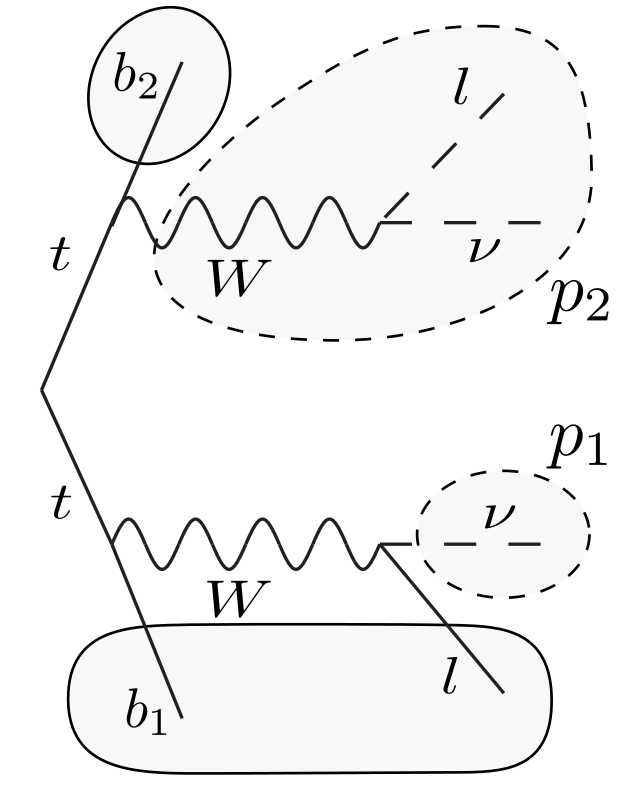
\includegraphics[width=0.33\linewidth]{Figures/mt2w_sketch.png}
\caption{\label{fig:mt2w_sketch}
Sketch of a dilepton \ttbar background event, dashed lines represent unseen
particles.}
\end{center}
\end{figure}

By cutting on a value larger than the top mass, this variable is very effective at removing the \ttbar lost lepton background.  Additionally, this variable has extended tails for signal hypotheses with large $\Delta$M between the stop and LSP.  Signal hypotheses with small $\Delta$M between the stop and LSP peak for masses smaller than the top mass.  Therefore, the search regions are classified into two types: \textit{High $\Delta$M} and \textit{Low $\Delta$M}, by cutting above and below a value just above the top mass. 

\begin{itemize}
  \item \textit{High $\Delta$M}: $\MTtW>200\GeV$
  \item \textit{Low $\Delta$M}: $\MTtW<200\GeV$
\end{itemize}


\subsubsection{ \MET}
\label{sec:obj_sel:met}

The \MET is calcuated as the vector sum of all PF candidates reconstructed in teh event.  The jet energy corrections described in section \ref{sec:obj_sel:jet_sel}.  

The LSP particles in the final state of the stop decay create additional \MET in the signal events.  This is one of the most powerful discriminanting variables in the search.  The signal regions are created from exclusive \MET bins beginning at $\MET>250\GeV$ in each of the \textit{High $\Delta$M} and \textit{Low $\Delta$M} classifications.  


\subsubsection{ Signal Region Definitions }
\label{sec:obj_sel:signal_regions}

A total of 9 signal regions are used in this search.  As described in section \ref{sec:obj_sel:met}, they are formed by creating exclusive \MET bins in the \textit{High $\Delta$M} and \textit{Low $\Delta$M} classifications.  They are listed below:

\begin{itemize}
  \item $nJets==3$, \textit{High $\Delta$M}: $\MTtW>200\GeV$
  \begin{itemize}
    \item $\MET>350 \GeV$
  \end{itemize}
  \item $nJets\ge4$, \textit{Low $\Delta$M}: $\MTtW<200\GeV$
  \begin{itemize}
     \item $250<\MET<325 \GeV$
     \item $\MET>325 \GeV$
  \end{itemize}
  \item $nJets\ge4$, \textit{High $\Delta$M}: $\MTtW>200\GeV$
  \begin{itemize}
     \item $250<\MET<350 \GeV$
     \item $350<\MET<450 \GeV$
     \item $\MET>450 \GeV$
  \end{itemize}
\end{itemize}



\section{Prediction from simulation}
\label{sec:MCyields}

A table of yields, for 2.11\fbinv, by production process, as well as by number of lepton decays in the hard process, and $Z\rightarrow\nu\nu$ is shown in table \ref{tab:MCyields}.

\begin{table}[htb]
\begin{center}
\caption{\label{tab:MCyields} Yields from simulation by production and decay process, for 2.11\fbinv. The uncertainties are only statistical.}
%\tiny
\begin{tabular}{|l|c|c|c|} 
\hline
sample/process & \multicolumn{3}{c|}{\MET selection} \\
\hline
 & Low $\Delta M$ & Low $\Delta M$ & Boosted High $\Delta M$ \\
 & $250 < \MET <325\GeV$ & $\MET>325\GeV$ & $\MET>350\GeV$ \\
 \hline
 Rare & 0.98 $\pm$ 0.08  & 0.53 $\pm$ 0.06 & 0.36 $\pm$ 0.07 \\
 W+jets  & 0.51 $\pm$ 0.23  & 0.40 $\pm$ 0.21 & 0.98 $\pm$ 0.43 \\
 Single t & 0.99 $\pm$ 0.27  & 0.58 $\pm$ 0.21 & 0.46 $\pm$ 0.19 \\
 $\ttbar\to1\ell$ & 0.67 $\pm$ 0.11  & 0.33 $\pm$ 0.08 & 0.05 $\pm$ 0.03 \\
 $\ttbar\to2\ell$ & 17.46 $\pm$ 0.54  & 7.46 $\pm$ 0.35 & 0.77 $\pm$ 0.12 \\
 \hline
 Total Background & 20.61 $\pm$ 0.66  & 9.30 $\pm$ 0.47 & 2.62 $\pm$ 0.49 \\ 
 \hline
 $1\ell$ & 1.33 $\pm$ 0.28  & 0.76 $\pm$ 0.22 & 1.10 $\pm$ 0.43 \\
 $\geq2\ell$ & 18.66 $\pm$ 0.59  & 8.21 $\pm$ 0.41 & 1.28 $\pm$ 0.23 \\
 $Z\to\nu\bar{\nu}$ & 0.62 $\pm$ 0.06  & 0.33 $\pm$ 0.05 & 0.23 $\pm$ 0.03 \\
 \hline
\multicolumn{4}{c}{~} \\[-1.5ex]
 \hline
 sample/process & \multicolumn{3}{c|}{\MET selection} \\
\hline
 & High $\Delta M$ & High $\Delta M$ & High $\Delta M$ \\
 & $250 < \MET <350\GeV$ & $350<\MET<450\GeV$ & $\MET>450\GeV$ \\
 \hline
Rare & 1.00 $\pm$ 0.10  & 0.52 $\pm$ 0.08  & 0.47 $\pm$ 0.08 \\
W+jets & 0.75 $\pm$ 0.17  & 0.71 $\pm$ 0.25  & 0.82 $\pm$ 0.42 \\
Single t & 0.93 $\pm$ 0.26  & 0.35 $\pm$ 0.16  & 0.24 $\pm$ 0.14 \\ 
 $\ttbar\to1\ell$  & 0.45 $\pm$ 0.09  & 0.13 $\pm$ 0.05  & 0.07 $\pm$ 0.04 \\ 
 $\ttbar\to2\ell$  & 3.21 $\pm$ 0.24  & 0.89 $\pm$ 0.12  & 0.66 $\pm$ 0.11 \\ 
 \hline 
Total Background & 6.34 $\pm$ 0.41  & 2.62 $\pm$ 0.34  & 2.26 $\pm$ 0.46 \\ 
\hline 
$1\ell$ & 1.59 $\pm$ 0.25  & 0.99 $\pm$ 0.27  & 1.05 $\pm$ 0.43 \\
 $\geq2\ell$  & 4.17 $\pm$ 0.33  & 1.30 $\pm$ 0.19  & 0.91 $\pm$ 0.16 \\
 $Z\to\nu\bar{\nu}$  & 0.59 $\pm$ 0.07  & 0.33 $\pm$ 0.05  & 0.30 $\pm$ 0.04 \\ 
 \hline
\end{tabular}
\end{center}
\end{table}

%\begin{table}
%\begin{center}
%\caption{\label{tab:MCyields} Yields by sample and production process, for 2.11\fbinv.}
%\tiny
%\begin{tabular}{|l|c|c|c|} \hline
%& $Low {\Delta}M, 250<MET<325$ & $Low {\Delta}M, MET>325$ \\ \hline \hline
%Rare & 0.98 $\pm$ 0.08  & 0.53 $\pm$ 0.06 \\ \hline
%$W$+Jets, madgraph & 0.51 $\pm$ 0.23  & 0.40 $\pm$ 0.21 \\ \hline
%DY+Jets, amcnlo & 0.00 $\pm$ 0.00  & 0.00 $\pm$ 0.00 \\ \hline
%Single $t$, powheg & 0.99 $\pm$ 0.27  & 0.58 $\pm$ 0.21 \\ \hline
%$t\bar{t}$, 1l, powheg ext & 0.67 $\pm$ 0.11  & 0.33 $\pm$ 0.08 \\ \hline
%$t\bar{t}$, 2l, powheg ext & 17.46 $\pm$ 0.54  & 7.46 $\pm$ 0.35 \\ \hline \hline
%Total Background & 20.61 $\pm$ 0.66  & 9.30 $\pm$ 0.47 \\ \hline \hline
%$==1$ lepton & 1.33 $\pm$ 0.28  & 0.76 $\pm$ 0.22 \\ \hline
%$\ge$2 lep & 18.66 $\pm$ 0.59  & 8.21 $\pm$ 0.41 \\ \hline
%$Z\rightarrow\nu\nu$ & 0.62 $\pm$ 0.06  & 0.33 $\pm$ 0.05 \\ \hline
%\end{tabular}
%
%\vspace{36pt}
%
%\begin{tabular}{|l|c|c|c|c|c|} \hline
%& $High {\Delta}M, ==3jets, MET>350$ & $High {\Delta}M, 250<MET<350$ & $High {\Delta}M, 350<MET<450$ & $High {\Delta}M, MET>450$ \\ \hline \hline
%Rare & 0.36 $\pm$ 0.07  & 1.00 $\pm$ 0.10  & 0.52 $\pm$ 0.08  & 0.47 $\pm$ 0.08 \\ \hline
%$W$+Jets, madgraph & 0.98 $\pm$ 0.43  & 0.75 $\pm$ 0.17  & 0.71 $\pm$ 0.25  & 0.82 $\pm$ 0.42 \\ \hline
%DY+Jets, amcnlo & 0.00 $\pm$ 0.00  & 0.00 $\pm$ 0.00  & 0.00 $\pm$ 0.00  & 0.00 $\pm$ 0.00 \\ \hline
%Single $t$, powheg & 0.46 $\pm$ 0.19  & 0.93 $\pm$ 0.26  & 0.35 $\pm$ 0.16  & 0.24 $\pm$ 0.14 \\ \hline
%$t\bar{t}$, 1l, powheg ext & 0.05 $\pm$ 0.03  & 0.45 $\pm$ 0.09  & 0.13 $\pm$ 0.05  & 0.07 $\pm$ 0.04 \\ \hline
%$t\bar{t}$, 2l, powheg ext & 0.77 $\pm$ 0.12  & 3.21 $\pm$ 0.24  & 0.89 $\pm$ 0.12  & 0.66 $\pm$ 0.11 \\ \hline \hline
%Total Background & 2.62 $\pm$ 0.49  & 6.34 $\pm$ 0.41  & 2.62 $\pm$ 0.34  & 2.26 $\pm$ 0.46 \\ \hline \hline
%$==1$ lepton & 1.10 $\pm$ 0.43  & 1.59 $\pm$ 0.25  & 0.99 $\pm$ 0.27  & 1.05 $\pm$ 0.43 \\ \hline
%$\ge$2 lep & 1.28 $\pm$ 0.23  & 4.17 $\pm$ 0.33  & 1.30 $\pm$ 0.19  & 0.91 $\pm$ 0.16 \\ \hline
%$Z\rightarrow\nu\nu$ & 0.23 $\pm$ 0.03  & 0.59 $\pm$ 0.07  & 0.33 $\pm$ 0.05  & 0.30 $\pm$ 0.04 \\ \hline
%\end{tabular}
%\end{center}
%\end{table}




\section{Background estimation methods}
\label{sec:bkgEstimation}

\subsection{Lost Lepton background}
\label{sec:bkgLL}

The lost lepton background represents the total background contribution from all physics processes that contain two or more leptons from the hard scatter process, where only one of the leptons is reconstructed in the event.  The mis-reconstruction of the second lepton can contribute to the \MET in the event. Additionally, the presence of a second neutrino provides a large tails in the \MT and \MTtW distributions.  This type of background is thus the largest background in the signal region.  

The $\ttjets$ process, where $t\bar{t}\rightarrow\ell\ell$, is the dominant contribution to this background.  The single $t$ process, produced in association with a $W$ boson, where both the $W$ and the $t$-quark decay to leptons, accounts for the second-largest contribution.  Addtional contributions come from ${\ttbar}V$ and diBoson processes.  

The following describes a data-driven method to estimate this background, using a control region enriched in dilepton events.  


\subsubsection{Estimation method from data}
\label{sec:bkgLL:Data}

The lost lepton background is estimated from data in a control region that requires a second lepton, passing the \textit{veto} requirements, or the presence of an isolated track or tau. After the Monte Carlo has been corrected for differences in lepton and jet reconstruction efficiencies, with respect to the data, the ratio of events in the control region and signal regions, should be equivalent between the observed and simulated number of events.  This relationship is shown in eq.~\ref{eq:diLep_CR_ratios}.

\begin{equation}\label{eq:diLep_CR_ratios}
\frac{N^{Data,~Signal~Region}_{\ell\ell}}{N^{Data,~Control~Region}_{\ell\ell}} = 
\frac{M^{MC,~Signal~Region}_{\ell\ell}}{M^{MC,~Control~Region}_{\ell\ell}}
\end{equation}

For the purpose of shortness, we will denote the number of data events by $N$ or $N^{Data}$, while we denote the number of simulated events by $M$ or $M^{MC}$. Also signal regions are denoted by $SR$, while dileptonic control regions are denoted by $CR$.

A data-driven estimate for the number of events in the signal regions, can then be calculated by re-arranging eq.~\ref{eq:diLep_CR_ratios} to eq.~\ref{eq:diLep_SR_est_simple}

\begin{equation}\label{eq:diLep_SR_est_simple}
N^{SR}_{\ell\ell} = N^{CR}_{\ell\ell}\times
\frac{M^{SR}_{\ell\ell}}{M^{CR}_{\ell\ell}}
\end{equation}

To prevent signal contamination in the tails of \MET, and increase the statistics available for the measurement in those regions, events in this control region are only binned in low and high \MTtW, ($<$200 GeV, and $\ge$200 GeV respectively), and uses an inclusive selection of gen lepton decays.  {\color{red} What do you mean with an inclusive selection of gen lepton decays - I would drop it}. 
An additional transfer factor is thus needed in eq.~\ref{eq:diLep_SR_est_full} to account for the binning in the jet multiplicity (nJets) and \MET found in the signal regions.  The final form of the diLepton background estimate is then written as:

\begin{equation}\label{eq:diLep_SR_est_full}
N^{Data,~SR}_{\ell\ell} = N^{Data,~CR}_{incl~in~gen~lepton~decays}\times
\frac{M^{MC,~SR}_{\ell\ell}}{M^{MC,~CR}_{incl~in~gen~lepton~decays}}\times
\frac{M^{MC,~SR}_{\ell\ell,~nJet,~\MET~bin}}{M^{MC,~SR}_{\ell\ell}}
\end{equation}

The uncertainty on the signal region estimate is dominated by the statistical uncertainty on the number of events measured in data 
in the control region. %, i.e. the first term in \ref{eq:diLep_SR_est_full}.  
%An additional benefit of c
Combining the nJet and \MET bins is reducing this uncertainty.  

Two of the most important aspects of exploiting the equivalence of the ratio between signal and control regions, is the modelling of additional 
jets due to ISR/FSR radiation, and the modelling of the \MET spectrum.  
Each play important roles in accurately calculating the transfer factor for nJet and \MET bins, but the additional jet modelling also comes 
into play in the differences between the signal and control regions as well. 
Therefore, a dedicated, low \MET, dilepton control region will be 
used to measure the jet multiplicity for $t\bar{t}$, and correct the simulation accordingly.      

\subsubsection{Addtional Control Region to Evaluate $t\bar{t}$ modelling}
\label{sec:bkgLL:emu_CR}

An additional control region is formed to study the simulation of the \ttjets background.  This region is used to derive an additional scale factor for the signal and control regions.  Approximately half the lost lepton background is composed of hadronic tau decays.  The other half, decays with a lost $e$ or $\mu$, need an additional ISR/FSR jet relative to the hadronic tau component of the lost lepton background, as shown in equation \ref{eq:emu_CR:xsecs}, in order to pass the jet selection requirements. 

%\begin{equation}
\begin{align} \label{eq:emu_CR:xsecs}
N^{SR}_{\ell\tau} &= (\sigma^{+1j}_{2\ell})\ast\epsilon_{reco~\ell}\ast(1-\epsilon_{reco~\tau})\ast\epsilon_{selection}\ast\epsilon_{reco~\tau~as~jet} \\
N^{SR}_{\ell\ell} &= (\sigma^{+2j}_{2\ell})\ast\epsilon_{reco~\ell}\ast(1-\epsilon_{reco~\ell})\ast\epsilon_{selection}
\end{align}
%\end{equation}

{\color{red} What is $\epsilon_{reco~\tau~as~jet}$. Basically every tau is a jet unless it is outside jet acceptance}.

Here, $\epsilon_{selection}$ is the total selection efficiency but the part coming from the leptons, which is encoded in the terms with $\epsilon_{reco~X}$.
For our signal regions, $\ttbar\to2\ell$ has - on tree level, just two jets in the event, while $\ttbar\to1\ell$ or signal has four jets (two jets from the hadronic W boson decay).

Events due to $\ttbar\to2\ell$, where the lost lepton is a hadronic tau, we need to find one additional ISR/FSR jet to pass our event selection, as the tau lepton itself is already identified as jet ($\rightarrow \sigma^{+1j}_{2\ell}$).
If however, the lost lepton is due to a missed e or $\mu$, we need at least two addition ISR/FSR jets ($\rightarrow \sigma^{+2j}_{2\ell}$).

When forming the ratio for the diLepton control region to the signal region (second factor in eq.~\ref{eq:diLep_SR_est_full}), 
the lepton reconstruction efficiencies will effectively cancel %due to their similarities in the denominator and numerator, 
and the only difference will be in the modelling of the cross section for additional ISR/FSR jets.  The scale factors are calculated as the 
ratio of ratios between data and Monte Carlo for jet bins of $=3/=2$ and $\ge4/=2$ jets.

The selection for this region is motivated to achieve a high-purity $t\bar{t}$ sample of events in data:

\begin{itemize}
  \item Pass an $e,\mu$ diLepton trigger
  %\begin{itemize}
   % \item HLT\_Mu17\_TrkIsoVVL\_Ele12\_CaloIdL\_TrackIdL\_IsoVL\_v*
   % \item HLT\_Mu23\_TrkIsoVVL\_Ele12\_CaloIdL\_TrackIdL\_IsoVL\_v*
  %\end{itemize}
  \item exactly 2 leptons
  \begin{itemize}
    \item e and $\mu$ flavour selection
    \item $\pt>30(15)\GeV$ leading (trailing) leptons 
    \item $|\eta|<2.1$
    \item POG ID medium (tight) for $e (\mu)$
    \item relative mini isolation $<0.1$
    \item oppositely charged
  \end{itemize}
  \item diLepton mass, $m_{\ell\ell}>20\GeV$
  \item nJets$\ge2$
  \item nBTags$\ge0$
\end{itemize}

We call this control region $CR_{e\mu}$. {color{red} Are you ok with that?}
The yields for this region are given in the following table \ref{tab:emu_CR:yields}.  Uncertainties are statistical only.  

\begin{table}[htb]
\begin{center}
\small
\caption{\label{tab:emu_CR:yields} Yield table for 2.11$fb^{1}$ of data for the $e,\mu$ control region, in bins of nTags}
\begin{tabular}{|l|c|c|c|c|} \hline
 & $CR_{e\mu},~\ge0~b-tags$ & $CR_{e\mu},~\ge1~b-tags$ & $CR_{e\mu},~\ge2~b-tags$ \\ \hline
Rare & 155.35 $\pm$ 1.28  & 30.33 $\pm$ 0.47  & 7.92 $\pm$ 0.21 \\ \hline
$W$+Jets, madgraph & 17.14 $\pm$ 1.71  & 2.97 $\pm$ 0.73  & 0.05 $\pm$ 0.02 \\ \hline
DY+Jets, amcnlo & 161.42 $\pm$ 17.86  & 22.07 $\pm$ 5.68  & 4.02 $\pm$ 2.34 \\ \hline
Single $t$, powheg & 403.17 $\pm$ 5.44  & 273.93 $\pm$ 4.38  & 64.94 $\pm$ 2.06 \\ \hline
$t\bar{t}$, 1l, powheg ext & 92.45 $\pm$ 1.28  & 52.74 $\pm$ 0.94  & 7.59 $\pm$ 0.35 \\ \hline
$t\bar{t}$, 2l, powheg ext & 7921.71 $\pm$ 11.85  & 6137.61 $\pm$ 10.21  & 2193.36 $\pm$ 5.85 \\ \hline
Total Background & 8751.32 $\pm$ 22.25  & 6519.69 $\pm$ 12.54  & 2277.90 $\pm$ 6.65 \\ \hline
Data & 8618  & 6333  & 2129 \\ \hline
Data/simulation & 0.98 $\pm$ 0.00  & 0.97 $\pm$ 0.00  & 0.93 $\pm$ 0.00 \\ \hline
\end{tabular}
\end{center}
\end{table}

The region of highest $t\bar{t}{\rightarrow}2\ell$ purity is the nBTags$\ge$2 category.  Therefore, this will be the region used to extract the correction factors for the $==3$ and $\ge4$ jet bins.  These factors will be applied to $t\bar{t}{\rightarrow}2\ell$ events in both the signal region, and nominal diLepton control region used to derive the signal estimate.   

The distributions of number of jets in each event, for increasing \MET cuts are shown in figure \ref{fig:bkgLostLepton:nJets}

\begin{figure}[ht]
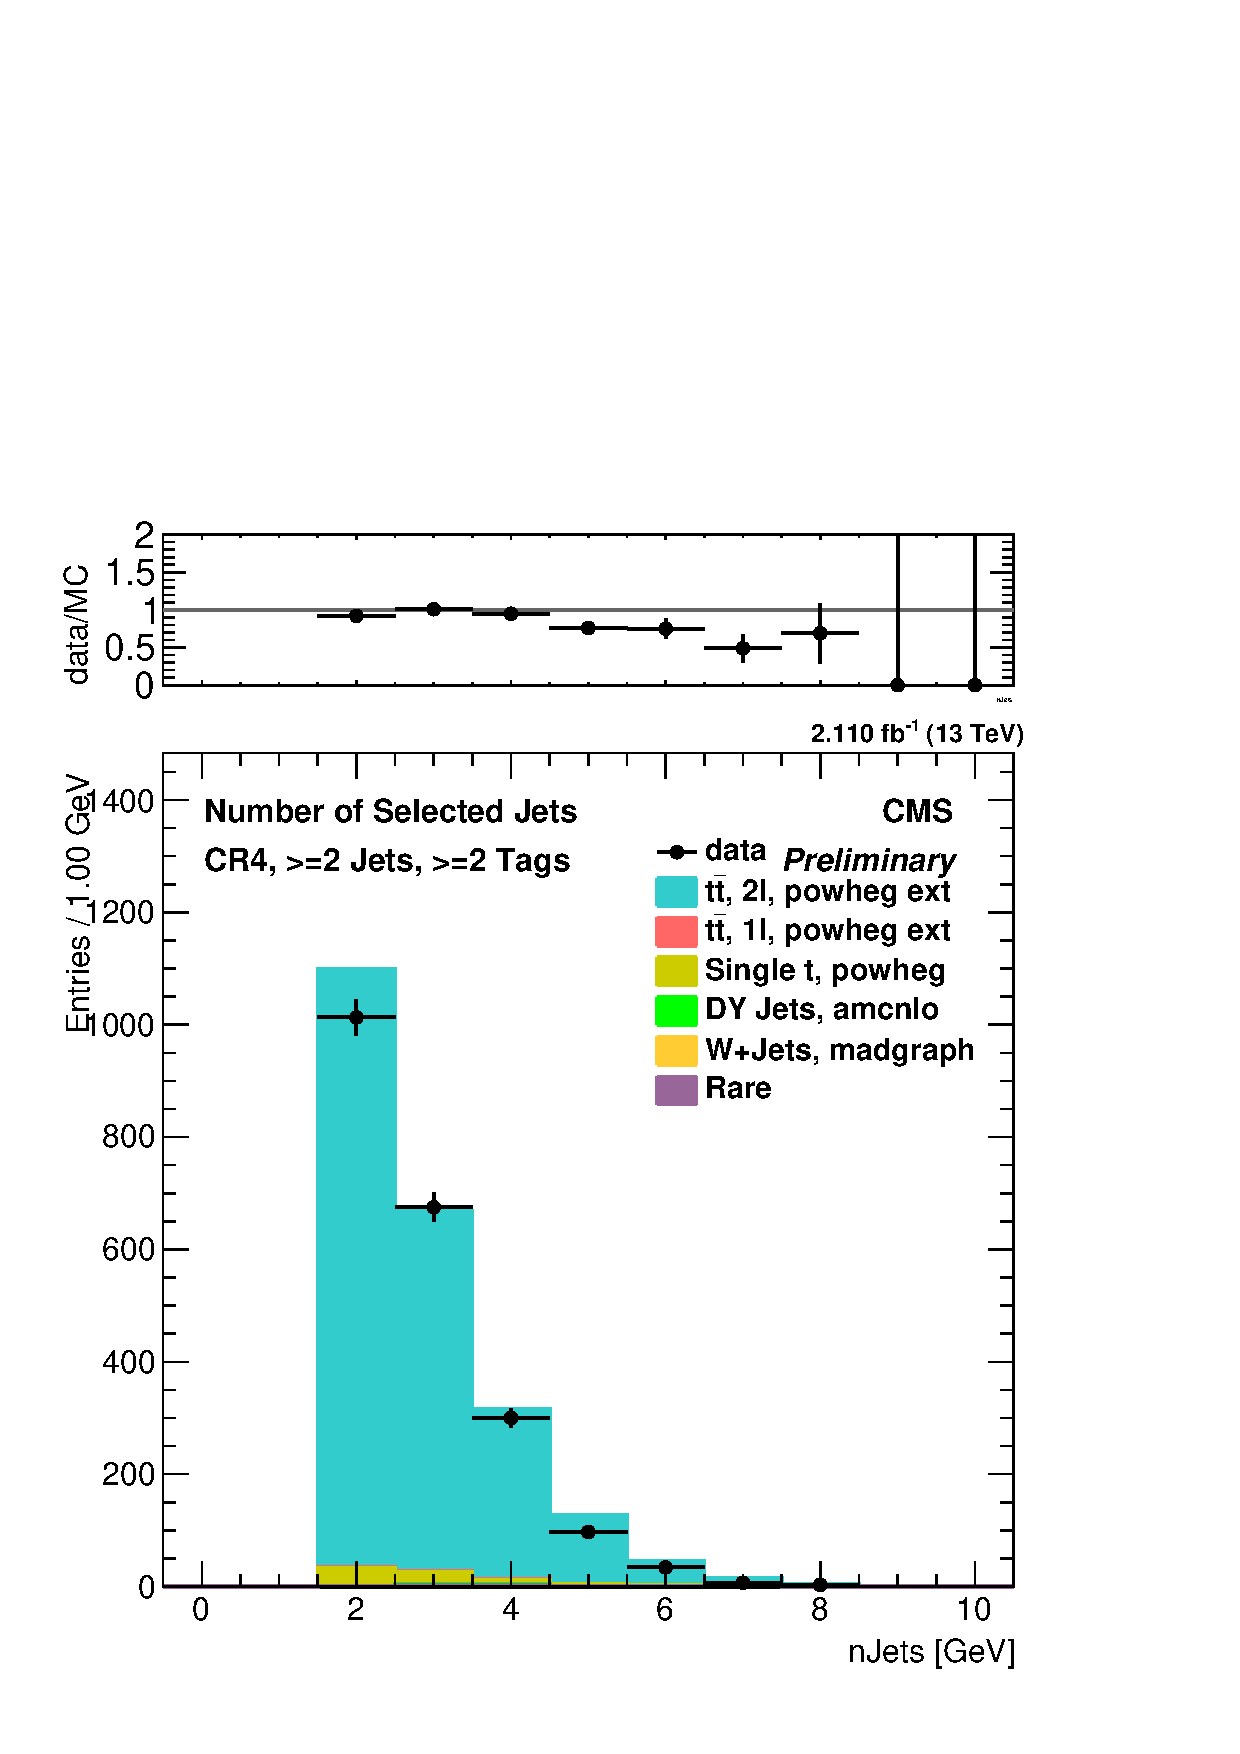
\includegraphics[width=0.32\textwidth]{Figures/bkgLostLepton/data_MC_plot__byProductionMode__nJets__elmu__ge2j_ge2t_gt0met__linScale.pdf}
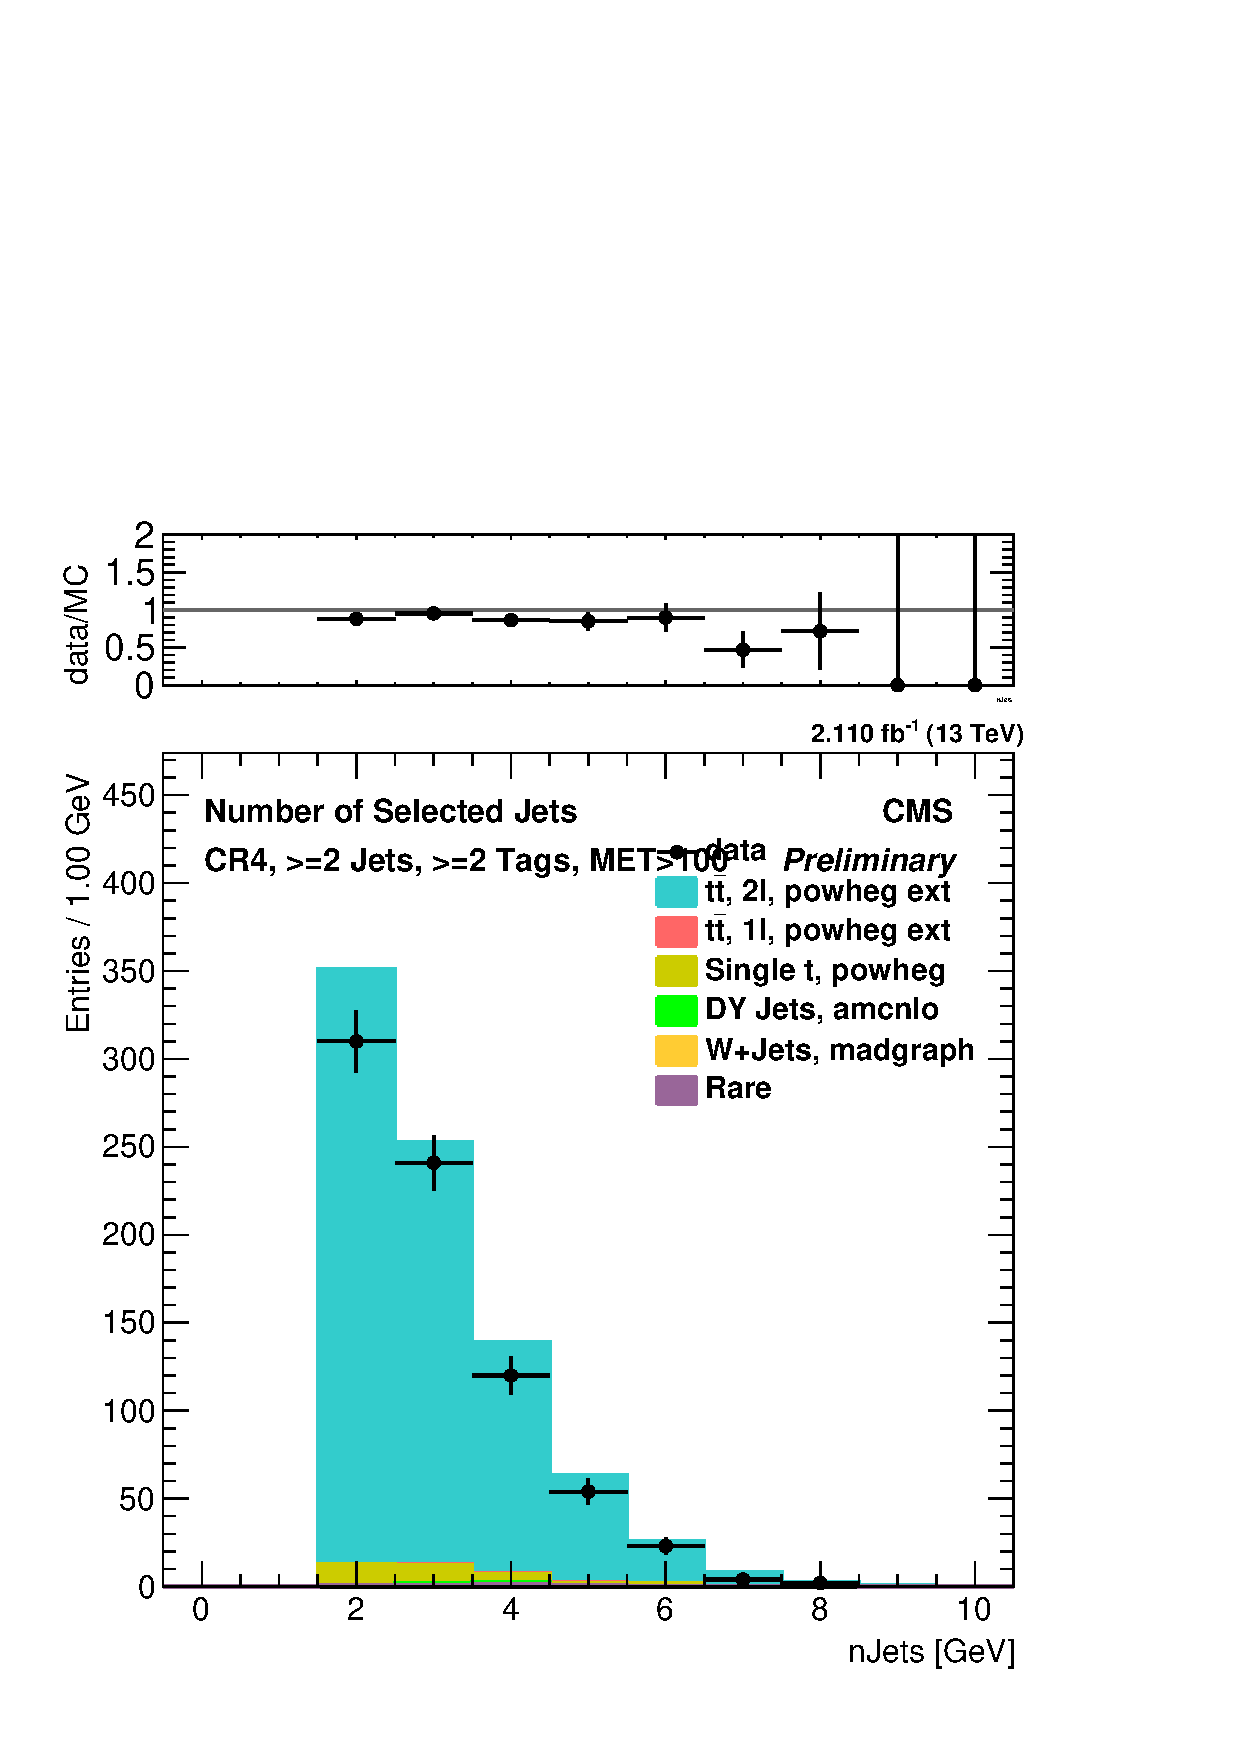
\includegraphics[width=0.32\textwidth]{Figures/bkgLostLepton/data_MC_plot__byProductionMode__nJets__elmu__ge2j_ge2t_gt100met__linScale.pdf}
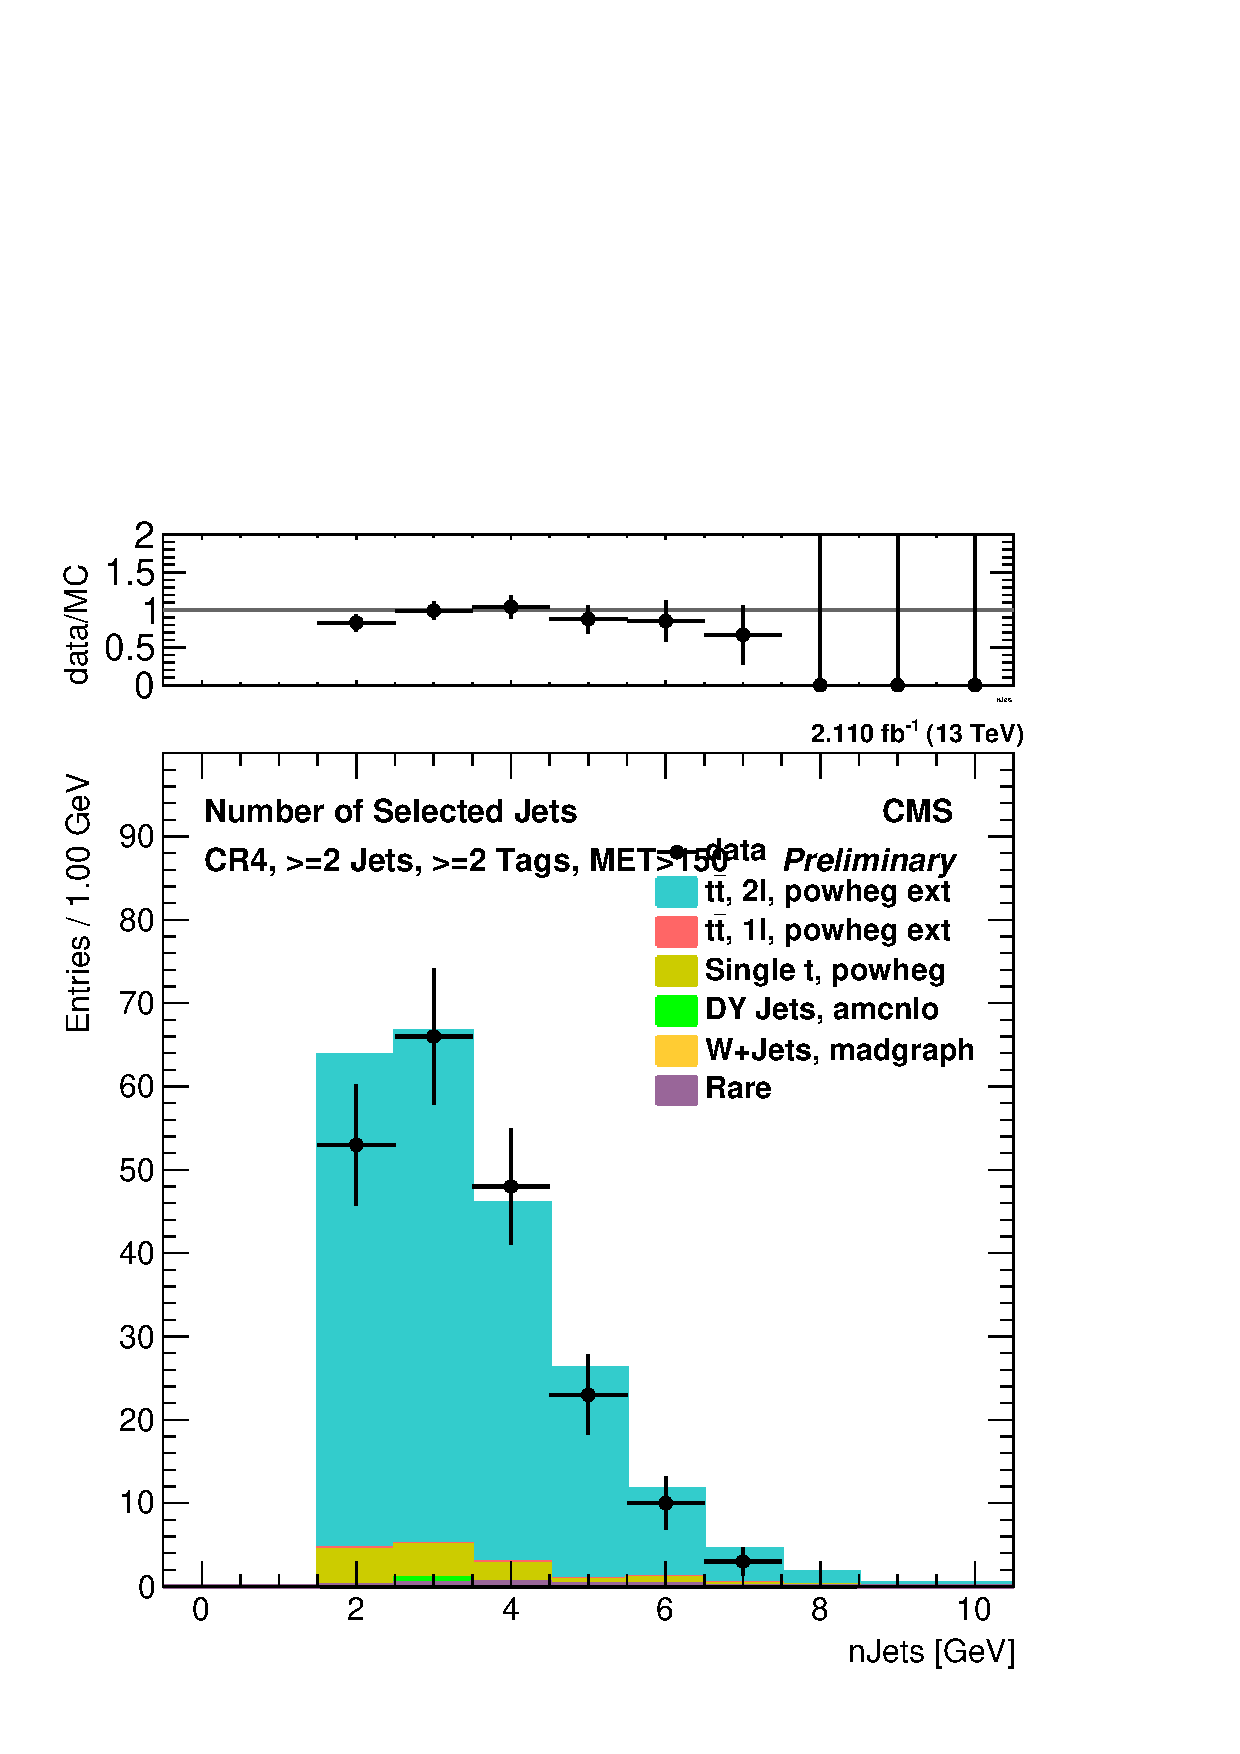
\includegraphics[width=0.32\textwidth]{Figures/bkgLostLepton/data_MC_plot__byProductionMode__nJets__elmu__ge2j_ge2t_gt150met__linScale.pdf}
\caption{\label{fig:bkgLostLepton:nJets} Distribution of number of jets for \MET$>$50 GeV (left), \MET$>$100 GeV (center), \MET$>$150 GeV}
\end{figure}

The scale factor derived from the nJets distribution in this region is given in table \ref{tab:emu_CR:SF}.  Within the statistical uncertainties quoted, the factors K3, and K4 are flat with increasing \MET. Thus, the most inclusive \MET bin will be used for the calculation, giving:

\begin{itemize}
  \item K3 = 1.10$\pm$0.06
  \item K4 = 0.94$\pm$0.06
\end{itemize}

\begin{table}[htb]
\begin{center}
\small
\caption{\label{tab:emu_CR:SF} Table of Scale Factors as a function \MET}
\begin{tabular}{|l|c|c|} \hline
Category & $nJets=3~(K_{3})$ & $nJets>=4~(K_{4})$ \\ \hline
$CR_{e\mu}, \ge2~b-tags, \MET\ge0\GeV$  & 1.10 $\pm$ 0.06 & 0.94 $\pm$ 0.06\\ \hline
$CR_{e\mu}, \ge2~b-tags, \MET>100\GeV$  & 1.08 $\pm$ 0.10 & 0.95 $\pm$ 0.09\\ \hline
$CR_{e\mu}, \ge2~b-tags, \MET>150\GeV$  & 1.21 $\pm$ 0.25 & 1.12 $\pm$ 0.22\\ \hline
$CR_{e\mu}, \ge2~b-tags, \MET>200\GeV$  & 1.42 $\pm$ 0.85 & 1.65 $\pm$ 0.89\\ \hline
\end{tabular}
\end{center}
\end{table}

%\subsubsection{High \MET diLepton Control Region used for Signal Region estimates}
\subsubsection{DiLepton Control Region used for Signal Region estimates}
\label{sec:bkgLL:highMET_CR}
 
As mentioned before, we estimate the lost lepton background by extrapolation 
in lepton veto, \MET, and Njets from appropriately chosen control regions.  
In the present section we document the control region definitions, control region yields, extrapolation
factors after all corrections, and the resulting estimates for lost lepton background yields in all signal regions.

We define two control regions (CR), one for MT2W$<$200 GeV, and one for MT2W$\ge$200 GeV.
For both region we require \MET $\ge$ 250 GeV, $\ge $ 3 jets, and one of the following lepton selections:

\begin{itemize}
    \item Require =2 leptons passing analysis selections, and $p_{T} >$ 20 GeV.
    \item Require =1 lepton passing analysis selection ($p_{T}>$ 20 GeV), and ==1 lepton passing veto selection ($p_{T}>$ 10 GeV).
    \item Require =1 lepton passing analysis selection, ==0 leptons passing veto selection, 
          and either an isolated track ($p_{T}>$ 10 GeV), or hardronic tau ($p_{T}>$ 20 GeV visible transverse momentum), 
          identified by the same requirements as the isolated track and tau vetoes.  
\end{itemize}

%This implies that there are exactly two control regions used to estimate the lost lepton backgrounds for all the signal regions.
The yields for both are given in the top two rows of Table \ref{tab:diLeptonType_Data_MC}.

In order to test the \MET modelling, we divide the some of those control region %\MET$\ge$ 250 GeV range 
into three subranges of roughly equal expected yield, and check
for any dependence of the Data/simulation yield ratio across \MET. We see no trend. %in this cross check. 
This is also documented in Table~\ref{tab:diLeptonType_Data_MC}.
Figure \ref{fig:cr_data_mc} provides a visual representation of the that table.  The uncertainties are statistical only. 
Additionally, the \MET and \MTtW distributions, are shown in figure \ref{fig:cr_data_mc:met_mt2w}.

\begin{table}[htb]
\begin{center}
\small
\caption{\label{tab:diLeptonType_Data_MC} Total event yields for each type of diLepton classification for data and MC, for 2.11$fb^{-1}$ }
\begin{tabular}{|l|c|c|c|} \hline
 Category & Data & MC & Data/MC \\ \hline
 $CR,~\ge3~jets,~\MET\ge250\GeV,~\MTtW<200\GeV$ & 66 $\pm$ 8.12 & 67.00 $\pm$ 1.14 & 0.99 $\pm$ 0.12 \\ \hline
 $CR,~\ge3~jets,~\MET\ge250\GeV,~\MTtW\ge200\GeV$ & 18 $\pm$ 4.24 & 25.55 $\pm$ 0.89 & 0.70 $\pm$ 0.17 \\ \hline\hline
 $CR,~\ge3~jets,~250<\MET<275\GeV$ & 27 $\pm$ 5.20 & 30.83 $\pm$ 0.80 & 0.88 $\pm$ 0.17 \\ \hline
 $CR,~\ge3~jets,~275<\MET<325\GeV$ & 31 $\pm$ 5.57 & 33.04 $\pm$ 0.86 & 0.94 $\pm$ 0.17 \\ \hline
 $CR,~\ge3~jets,~\MET>325\GeV$ & 26 $\pm$ 5.10 & 28.69 $\pm$ 0.85 & 0.91 $\pm$ 0.18 \\ \hline
\end{tabular}
\end{center}
\end{table}

\begin{figure}[ht]
\centering
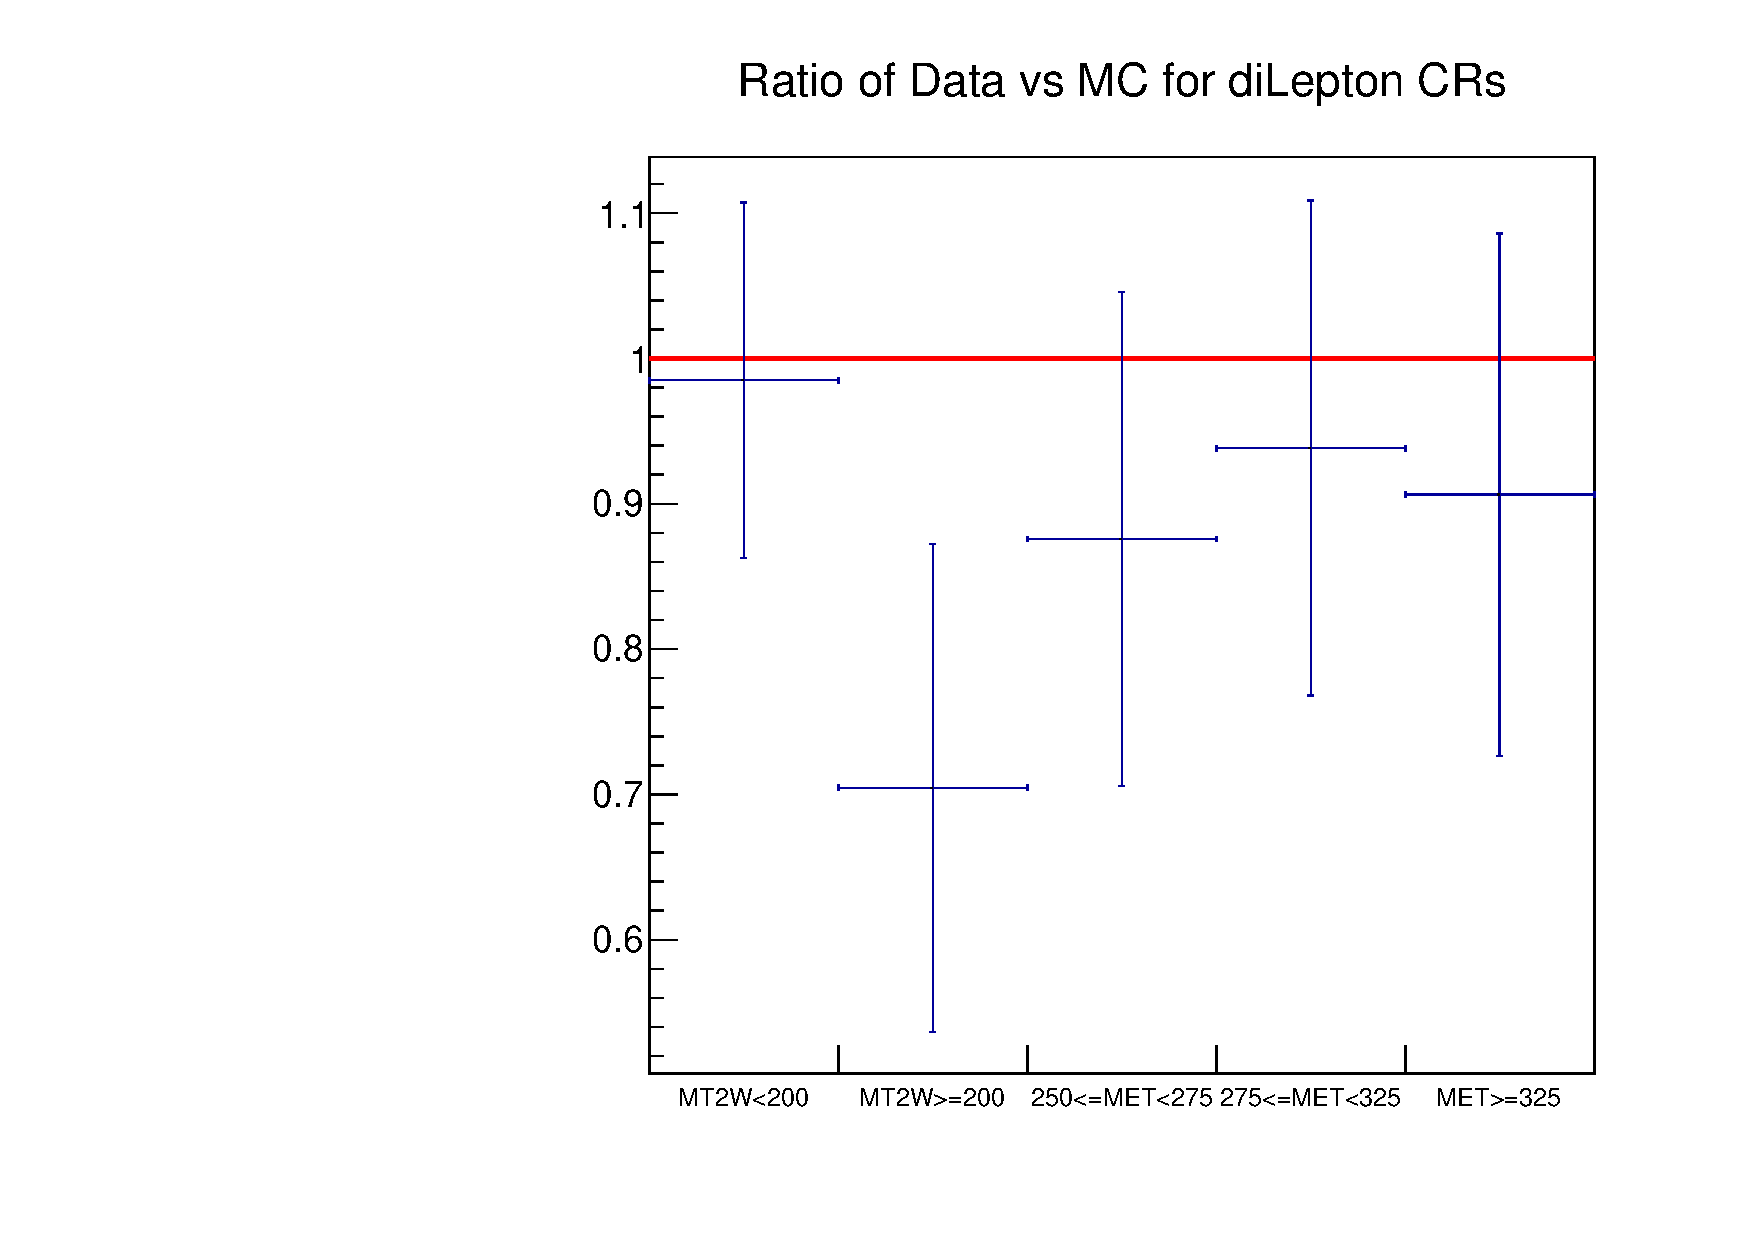
\includegraphics[width=0.70\textwidth]{Figures/bkgLostLepton/data_vs_mc__diLep_CR4_5_6__ge3j__ge250met__ratioOfCRs.pdf}
\caption{\label{fig:cr_data_mc} Data vs MC comparisons of the 5 bins used to evaluate the control region}
\end{figure}


\begin{figure}[ht]
\centering
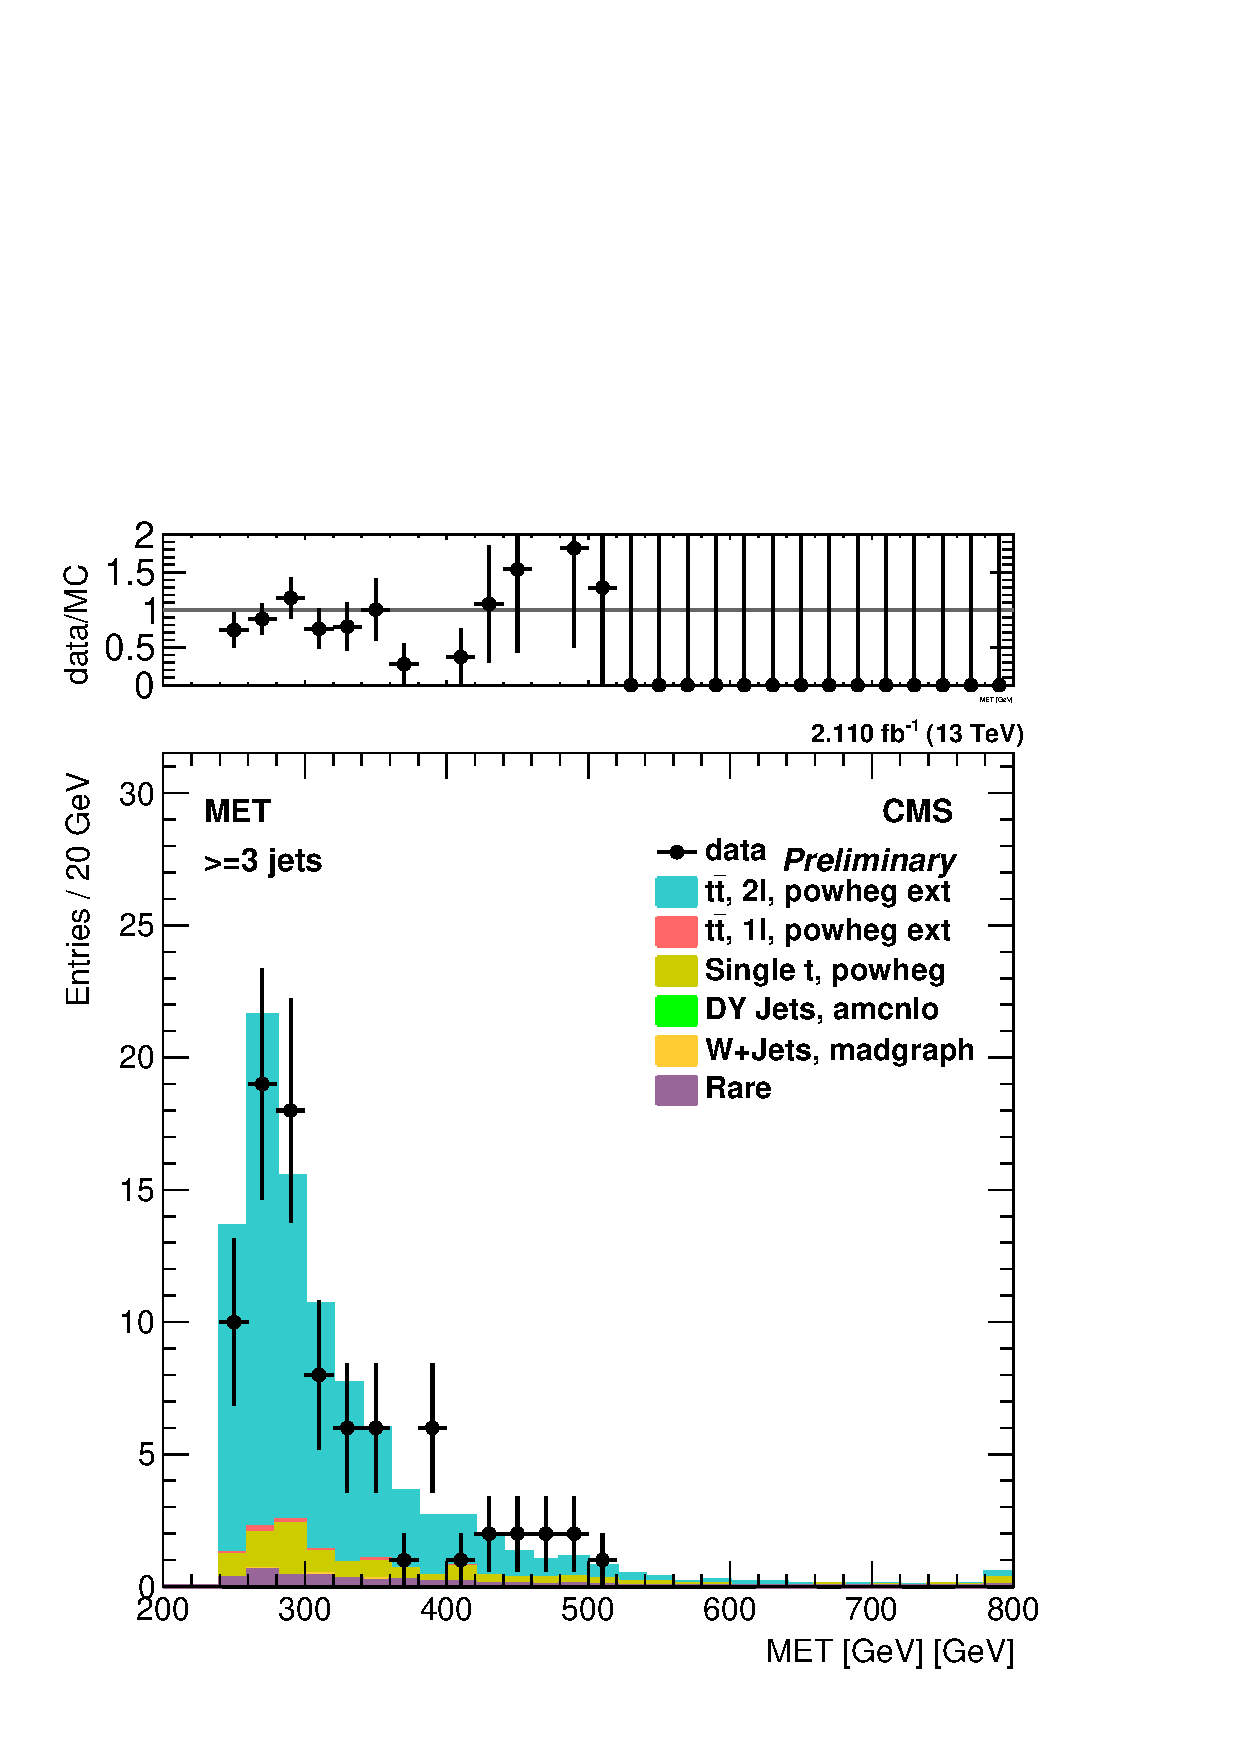
\includegraphics[width=0.45\textwidth]{Figures/bkgLostLepton/data_MC_plot__byProductionMode__met__ge3j_ge250met__linScale.pdf}
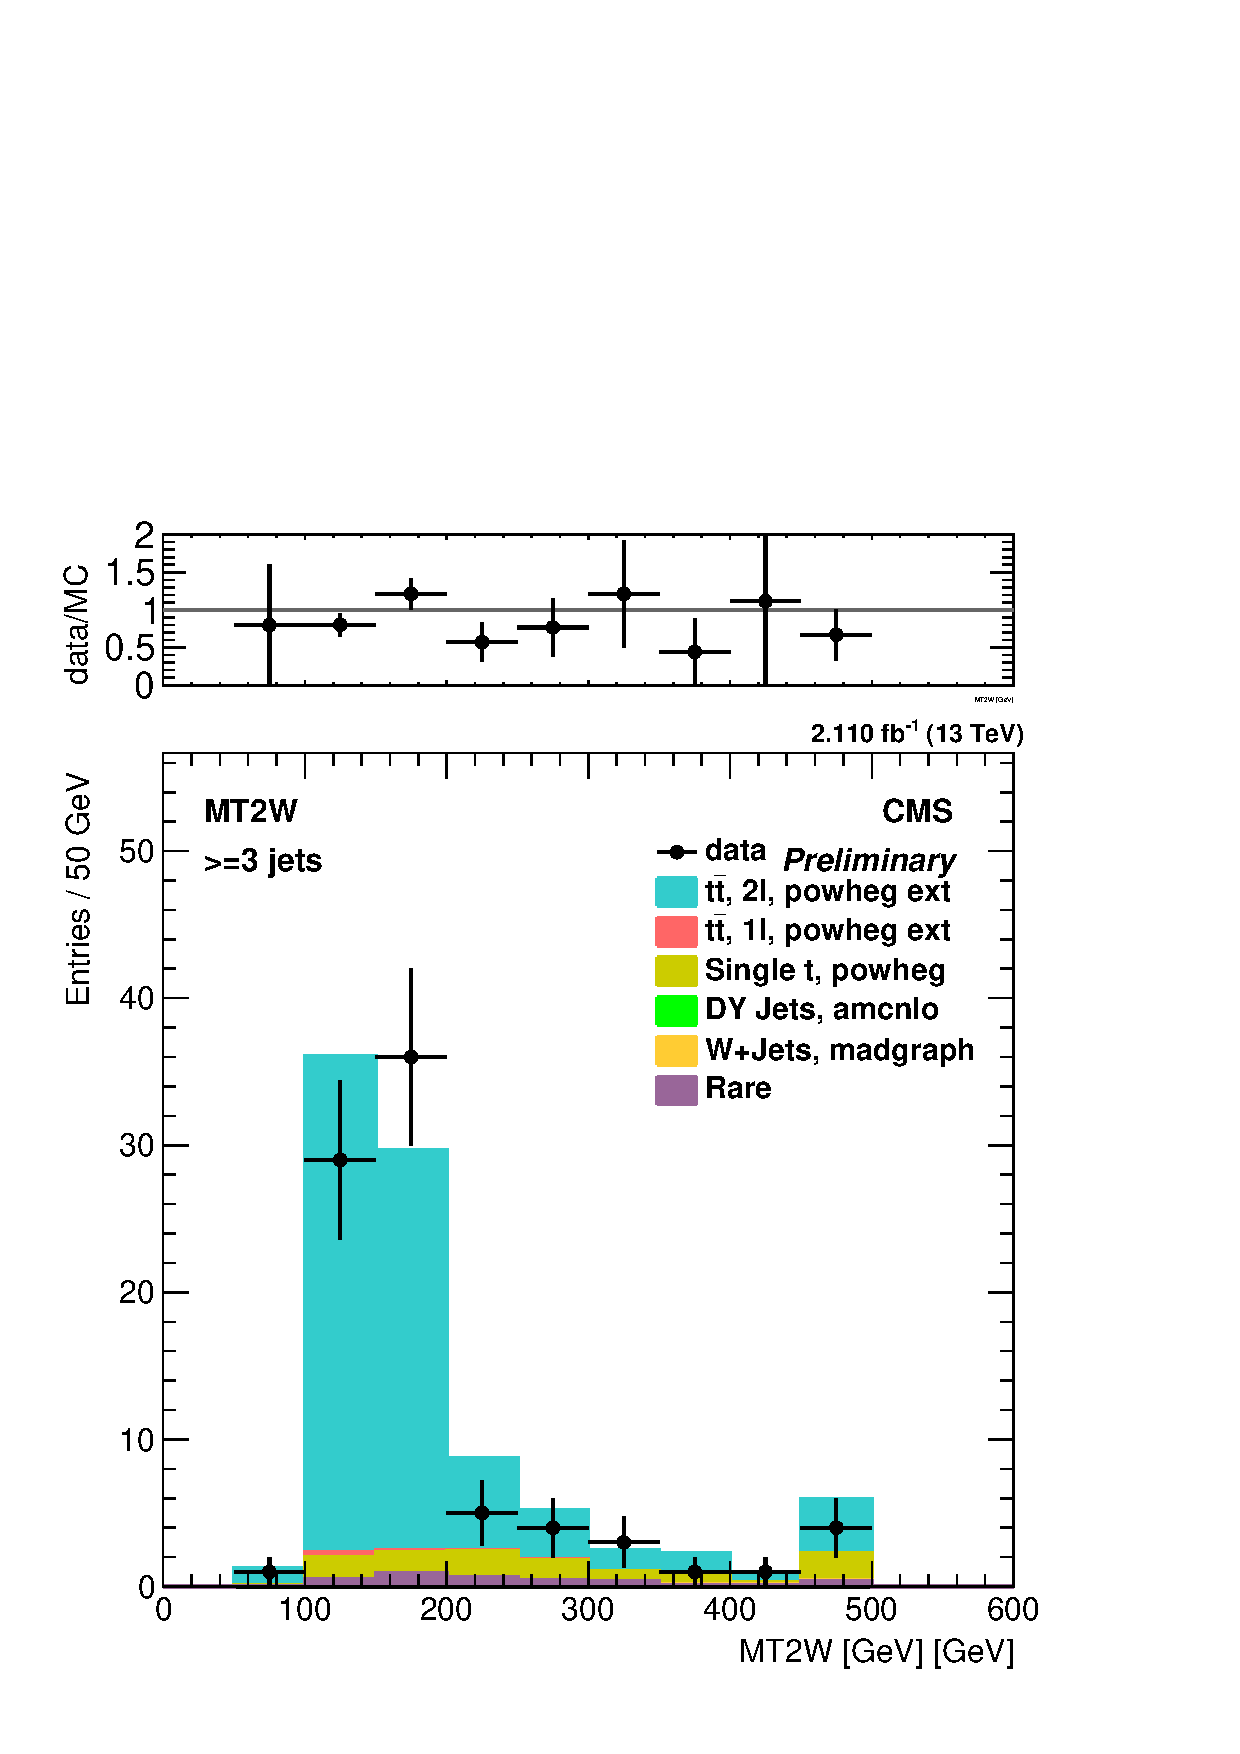
\includegraphics[width=0.45\textwidth]{Figures/bkgLostLepton/data_MC_plot__byProductionMode__mt2w__ge3j_ge250met__linScale.pdf}
\caption{\label{fig:cr_data_mc:met_mt2w} Distribution of \MET and MT2W in the diLepton CR}
\end{figure}


The resulting background yield predictions for each signal region are described in table \ref{tab:sr_estimate_lostLep}.  
The uncertainties here include the full systematic uncertainties from lepton, jet, and bTagging scale factors, 
as well as acceptance uncertainties from $Q^{2}$ and $\alpha_{S}$ variations, that are described in more detail in the 
following section.

%\subsubsection{High \MET diLepton Control Region used for Signal Region estimates, Systematic Uncertainties}
\subsubsection{Systematic Uncertainties for the lost lepton background estimation}
\label{sec:bkgLL:highMET_CR:systematics}

The full list of systematics used to evaluate the uncertainty on the diLepton background estimate is shown in table \ref{tab:ll_estimate_sysUnc_summary}.  

\begin{table}[htb]
\begin{center}
\small
\caption{\label{tab:ll_estimate_sysUnc_summary} Table of uncertainties for the diLepton background estimate, range for smallest-largest variation in each signal region. }
\scalebox{0.9}{
\begin{tabular}{|l|c|c|c|c|} \hline
Systematic & $N_{Incl}^{CR}~(\%)$ & $M_{2\ell}^{SR}/M_{Incl}^{CR}~(\%)$ & $M_{MET,nJet~bin}^{SR}/M_{2\ell}^{SR}~(\%)$ & $N_{2\ell,estimate}^{SR}~(\%)$ \\ \hline \hline
%Data Stats & $12.3~-~23.6~\%$ & $0.0~-~0.0~\%$ & $0.0~-~0.0~\%$ & $12.3~-~23.6~\%$ \\ \hline
%MC Stats & $0.0~-~0.0~\%$ & $1.7~-~3.5~\%$ & $2.1~-~11.6~\%$ & $2.7~-~12.1~\%$ \\ \hline
%$Luminosity$ & $0.0~-~0.0~\%$ & $0.0~-~0.0~\%$ & $0.0~-~0.0~\%$ & $0.0~-~0.0~\%$ \\ \hline
%$bTag~Efficiency,~Heavy~Flavour$ & $0.0~-~0.0~\%$ & $0.3~-~0.3~\%$ & $0.0~-~1.3~\%$ & $0.2~-~1.5~\%$ \\ \hline
%$bTag~Efficiency,~Light~Flavour$ & $0.0~-~0.0~\%$ & $1.4~-~2.1~\%$ & $0.0~-~0.9~\%$ & $0.9~-~2.3~\%$ \\ \hline
%$lepton~SF$ & $0.0~-~0.0~\%$ & $3.9~-~4.3~\%$ & $0.1~-~3.7~\%$ & $3.2~-~8.0~\%$ \\ \hline
%$top~p_{T}~SF$ & $0.0~-~0.0~\%$ & $0.3~-~2.8~\%$ & $0.2~-~13.5~\%$ & $0.2~-~13.7~\%$ \\ \hline
%$nJets~SF,~K3,~K4$ & $0.0~-~0.0~\%$ & $0.1~-~0.6~\%$ & $0.1~-~1.3~\%$ & $0.2~-~1.1~\%$ \\ \hline
%$PDF$ & $0.0~-~0.0~\%$ & $0.2~-~0.6~\%$ & $0.1~-~0.7~\%$ & $0.0~-~1.2~\%$ \\ \hline
%$\alpha_{S}$ & $0.0~-~0.0~\%$ & $0.1~-~0.4~\%$ & $0.0~-~0.5~\%$ & $0.0~-~0.6~\%$ \\ \hline
%$Q^{2}$ & $0.0~-~0.0~\%$ & $0.3~-~4.1~\%$ & $0.4~-~8.4~\%$ & $0.4~-~12.9~\%$ \\ \hline
%JES & $0.0~-~0.0~\%$ & $0.4~-~4.1~\%$ & $1.1~-~11.5~\%$ & $1.5~-~8.3~\%$ \\ \hline \hline
%Total & $12.3~-~23.6~\%$ & $5.6~-~8.2~\%$ & $3.6~-~20.1~\%$ & $14.6~-~34.0~\%$ \\ \hline
Data Statistics & $12.3~-~23.6~\%$ & --- & --- & $12.3~-~23.6~\%$ \\ \hline
Simulation Statisticss & --- & $1.7~-~3.5~\%$ & $2.1~-~11.6~\%$ & $2.7~-~12.1~\%$ \\ \hline
%Luminosity & --- & --- & --- & --- \\ \hline
bTag~Efficiency,~Heavy~Flavour & --- & $0.3~-~0.3~\%$ & $0.0~-~1.3~\%$ & $0.2~-~1.5~\%$ \\ \hline
bTag~Efficiency,~Light~Flavour & --- & $1.4~-~2.1~\%$ & $0.0~-~0.9~\%$ & $0.9~-~2.3~\%$ \\ \hline
lepton~SF & --- & $3.9~-~4.3~\%$ & $0.1~-~3.7~\%$ & $3.2~-~8.0~\%$ \\ \hline
top~\pt~SF & --- & $0.3~-~2.8~\%$ & $0.2~-~13.5~\%$ & $0.2~-~13.7~\%$ \\ \hline
nJets~SF,~K3,~K4 & --- & $0.1~-~0.6~\%$ & $0.1~-~1.3~\%$ & $0.2~-~1.1~\%$ \\ \hline
PDF & --- & $0.2~-~0.6~\%$ & $0.1~-~0.7~\%$ & $0.0~-~1.2~\%$ \\ \hline
$\alpha_{S}$ & --- & $0.1~-~0.4~\%$ & $0.0~-~0.5~\%$ & $0.0~-~0.6~\%$ \\ \hline
$Q^{2}$ & --- & $0.3~-~4.1~\%$ & $0.4~-~8.4~\%$ & $0.4~-~12.9~\%$ \\ \hline
JES & --- & $0.4~-~4.1~\%$ & $1.1~-~11.5~\%$ & $1.5~-~8.3~\%$ \\ \hline \hline
Total & $12.3~-~23.6~\%$ & $5.6~-~8.2~\%$ & $3.6~-~20.1~\%$ & $14.6~-~34.0~\%$ \\ \hline
\end{tabular}
}
\end{center}
\end{table}



The uncertainties are described as follows:
\begin{itemize}
  \item Data and MC statisitics - the largest uncertainty is due to the statistical error on the observed control region yields in data.
  \item nJets K3, K4 - impact of the statistical errors on the nJets scale factors applied to $\ttbar\to2\ell$, as described in the previous section. 
  \item bTagging Heavy/Light Flavour, SF - the variation of the heavy/light flavour component of the bTagging reweighting, as provided by the BTV POG.
%  \item bTagging Light Flavour, SF - the variation of the light flavour component of the bTagging reweightingm as provided by the BTV POG.
  \item lepton SF - the varation of the lepton scale factors, as provided by the SUSY group.  Scale factors for both ID and isolation are applied.
  \item top pT  - although the reweighting is not applied as a scale factor, an additional uncertainty is taken to account for the difference in yields if the reweighting is applied, as recommended by the top PAG. 
  \item PDF - the method used is to take the average of 100 different PDF variations, and use the standard deviation of this average to vary the acceptance on the MC
  \item $\alpha_{S}$ - this method varies the QCD scale of the event to change the acceptance. 
  \item $Q^{2}$ - the largest two variations in renormalization and factorization scale are taken as an envelope.  
  \item JES - the jet energy scale is varied, to account for diffences in jet acceptance.  
\end{itemize}

The latter uncertainties only consider the change in acceptance, but not in cross-section as we obtain the cross section from the data yields.

Even, if we write out the estimation formula as in eq.~\ref{eq:diLep_SR_est_full}, we do not double count uncertainties due to cancelling terms in that equation.

{\bf fkw comment: We are still missing the impact of possible \MET resolution difference between data and MC on
     possible bin migration in \MET,and corresponding impact on the \MET extrapolation. I.e. this is HJ's photon sample
     technique applied to the lost lepton bkg estimate. I thought we decided to do this at our f2f meeting at fnal.}
{\color{red} HJ: Do we need this here. We thought the main contribution of the \MET shape is due to real \MET. Possible mismodelling should (partially) taken care of JES. Anyway, I think John is implementing it, and as soon as it is in, I'll add a short paragraph, with forward-reference to the WJets section.}

\subsection{Results of the lost lepton background estimation}
\label{sec:bkgLL:highMET_CR:results}

\begin{table}[htb]
\begin{center}
\small
\caption{\label{tab:sr_estimate_lostLep} Total event yields for each type of diLepton classification for data and MC, for 2.11\fbinv. }
\begin{tabular}{|l|l|c|c|c|c|} \hline
region & \MET & $N_{Incl}^{CR}$ & $M_{2\ell}^{SR}/M_{Incl}^{CR}$ & $M_{MET,nJet}^{SR}/M_{2\ell}^{SR}$ & $N_{2\ell,estimate}^{SR}$\\ \hline
 Low ${\Delta}M$ & $250<\MET<325\GeV$ & 66 $\pm$ 8.12 & 0.61 $\pm$ 0.03 & 0.46 $\pm$ 0.02 & 18.39 $\pm$ 2.69 \\ \hline
 Low ${\Delta}M$ & $\MET>325\GeV$ & 66 $\pm$ 8.12 & 0.61 $\pm$ 0.03 & 0.20 $\pm$ 0.02 & 8.09 $\pm$ 1.34 \\ \hline
 Boosted High ${\Delta}M$ & $\MET>350\GeV$ & 18 $\pm$ 4.24 & 0.44 $\pm$ 0.04 & 0.11 $\pm$ 0.02 & 0.90 $\pm$ 0.25 \\ \hline
 High ${\Delta}M$ & $250<\MET<350\GeV$ & 18 $\pm$ 4.24 & 0.44 $\pm$ 0.04 & 0.37 $\pm$ 0.02 & 2.94 $\pm$ 0.78 \\ \hline
 High ${\Delta}M$ & $350<\MET<450\GeV$ & 18 $\pm$ 4.24 & 0.44 $\pm$ 0.04 & 0.12 $\pm$ 0.01 & 0.91 $\pm$ 0.25 \\ \hline
 High ${\Delta}M$ & $\MET>450\GeV$ & 18 $\pm$ 4.24 & 0.44 $\pm$ 0.04 & 0.08 $\pm$ 0.02 & 0.64 $\pm$ 0.22 \\ \hline
\end{tabular}
\end{center}
\end{table}


\subsection{One Lepton background}
\label{sec:bkgOL}

%In this analysis, the SM backgrounds with one real lepton in the final state come from W decays, either through direct W production or W boson��s 
In this analysis, the SM backgrounds with one real lepton in the final state come from W decays, either through direct W production of W bosons
from top decays.  The neutrino from the W decay is the source of real \MET, potentially smeared out due to resolution effects.
%
Given our baseline requirements of \MET $\ge $ 250\GeV and \MT$\ge$ 150\GeV, this background is dominated by direct W production.
We can thus estimate it by extrapolating from zero b-tag control regions. 
For MT2W$\ge $ 200 GeV, we choose two such regions, both with \MET$\ge$ 250\GeV, one for exactly 3 jets, and one for $\ge$ 4 jets.
For MT2W$<$ 200 GeV, even a potential zero b-tag control region would be dominated by lost lepton background. 
Furthermore, the one lepton background accounts for
less than 10\% of the total background for MT2W$<$ 200\GeV, and a data driven estimate is thus not warranted.
%
Similarily, the one lepton background from ttbar is a sufficiently small fraction of the total background that
it does not warrant a data driven estimate.

In the following, we first describe in detail the data driven estimate for the W jets background, including its systematic error, and then
conclude with Tables of the total one lepton background, including the parts taken from simulation. Additional details on the latter are provided
in the Appendix. The Appendix also includes crosschecks in data to further justify the conclusion that one lepton background from W's from top
decay is always small compared to other sources of background.
  
\subsubsection{Estimation Method from Data}
\label{subsec:bkg1L:Data}

Our control region to signal region extrapolation for the W plus jets background is based on the following assumption:

\begin{equation}\label{eq:btag_CR_ratios}
\frac{N^{data}_{0-btag}}{N^{data}_{\ge1-btag}} = \frac{N^{MC}_{0-btag}}{N^{MC}_{\ge1-btag}}
\end{equation}

Eq. ~\ref{eq:btag_CR_ratios} allows us to use normalize the background estimate in data in a 0-btag region, and then use simulation
to extrapolate from there to the corresponding $\ge$ 1 b-tag signal region as follows:
%
\begin{equation}\label{eq:btag_CR_ratios2}
N^{W+Jets}_{SR,\ge1-btag} = N^{data,WJets}_{CR,0-btag} \times \frac{N^{MC,WJets}_{SR,\ge1-btag}}{N^{MC,WJets}_{CR,0-btag}}
\end{equation}
%
Here $N^{data,WJets}_{SR,\ge 1-btag}$ is the estimated W+Jets contribution to each SR, 
$N^{data,WJets}_{0-btag}$ is the number of W+Jets events according to data in the CR, 
and ${N^{MC,WJets}_{\ge1-btag}}{N^{MC,WJets}_{0-btag}}$ is the 0-btag to 1-btag extrapolation factor.  
To obtain $N^{data,WJets}_{0-btag}$, we take the total data yield in the CR and subtract the 
non-WJets contribution according to MC prediction:
\begin{equation}\label{eq:wjetsyield}
N^{data,WJets}_{CR,0-btag} = N^{data}_{CR,0-btag} - N^{non-WJets MC}_{CR,0-btag}
\end{equation}

In practice, we do not have sufficient statistics in the zero b-tag sample to form a dedicated CR for every SR.
As a compromise between statistical and systematic error, we define two such W+jets CRs as follows:
\begin{itemize}
\item CR1:  0-btags, \MET $>$ 250 GeV, exactly 3 jets to estimate W+Jets for the 3 jet SRs.
\item CR2:  0-btags, \MET $>$ 250 GeV, $\ge$ 4 jets to estimate W+Jets for the $\ge$ 4 jets SRs.
\end{itemize}
This implies that we employ a second extrapolation in \MET from our inclusive \MET$\ge$ 250 \GeV baseline region to
the various exclusive \MET bins. 

We define the two aforementioned extrapolation factors as follows:
%
\begin{equation}\label{eq:tfmet}
TF_{MET}(\MET, njets) = \frac{N^{MC,WJets}_{0-btag}(\MET,njets)}{N^{MC,WJets}_{0-btag,\MET>250}(njets)}
\end{equation}
%
\begin{equation}\label{eq:tfbtag}
TF_{btag}(\MET, njets) = \frac{N^{MC,WJets}_{\ge1-btag,SR}(\MET,njets)}{N^{MC,WJets}_{0-btag,CR}(\MET,njets)}
\end{equation}
%
$TF_{MET}$ extrapolates only in \MET at fixed jet multiplicity and for the zero b-tag distributions, while
$TF_{btag}$ extrapolates only in the number of b-tags at fixed \MET and fixed jet multiplicity.

\subsubsection{Data versus MC Crosschecks of the \MET distribution}\label{subsec:METStudy}

{\bf fkw comments: I don't see why we keep this in the main text. I would put this into the appendix as it is in no way used to derive the actual background estimate.}

As discussed in Section~\ref{sec:bkgOL}, we use the simulation to extrapolate in \MET from an inclusive region \MET $\ge$ 250 \GeV into
into multiple inclusive \MET bins. In the present section we provide several data vs MC comparison of \MET distributions in 
zero b-tag control regions as crosschecks for this extrapolation.
These W+Jets CRs are summarized in Table~\ref{tab:WJetsCRsMET} and the corresponding \MET distributions are shown in Figures~\ref{fig:METDist}. 

\begin{figure}[h]
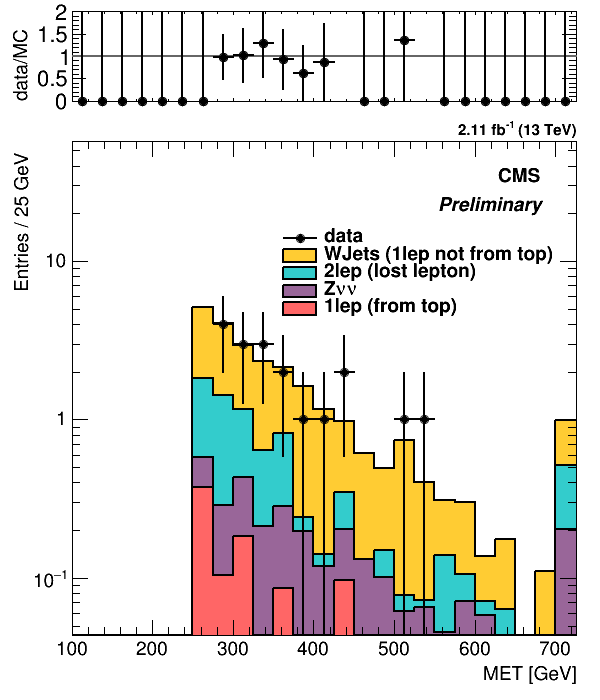
\includegraphics[width=0.44\textwidth]{Figures/bkg1lep/MET_MET250_MT120_4jets.png}
%\includegraphics[width=0.32\textwidth]{Figures/bkg1lep/MET_MET250_MTband_4jets.png}
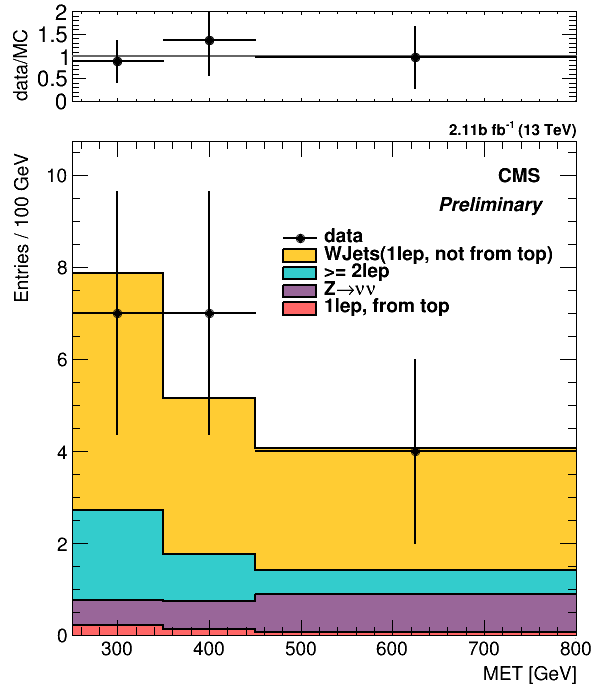
\includegraphics[width=0.44\textwidth]{Figures/bkg1lep/MET_MET250_MT150_4jets.png}
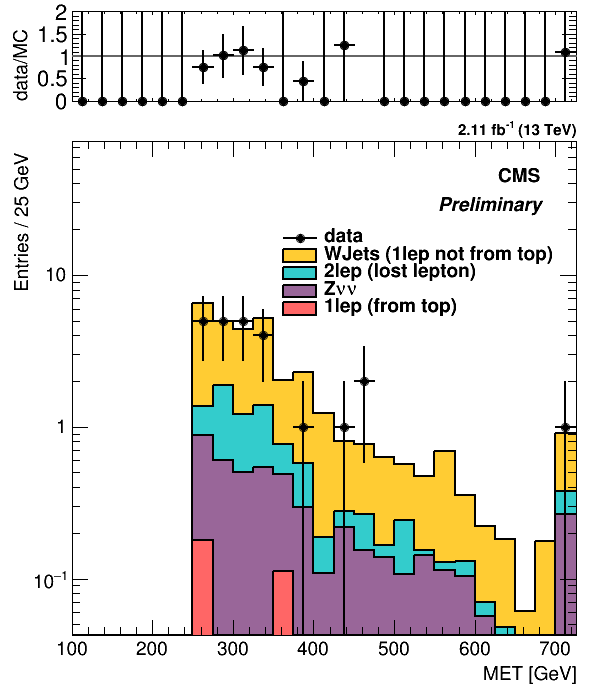
\includegraphics[width=0.44\textwidth]{Figures/bkg1lep/MET_MET250_MT120_3jets.png}
%\includegraphics[width=0.32\textwidth]{Figures/bkg1lep/MET_MET250_MTband_3jets.png}
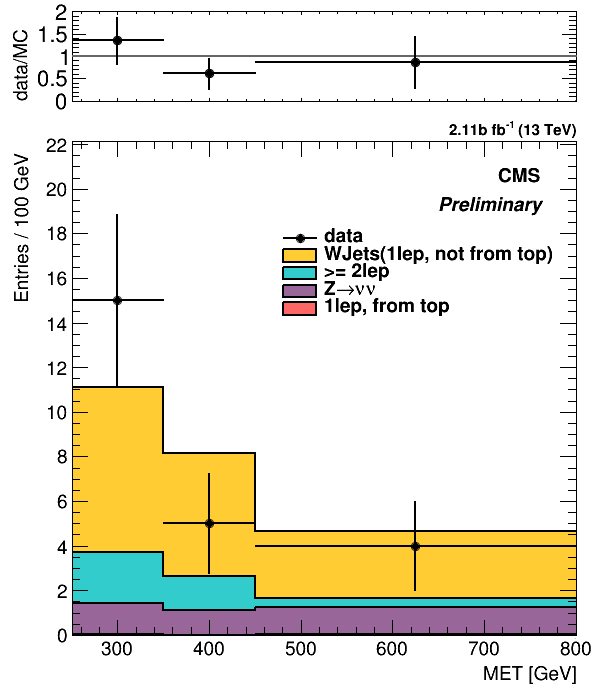
\includegraphics[width=0.44\textwidth]{Figures/bkg1lep/MET_MET250_MT150_3jets.png}
\caption{\label{fig:METDist} Distribution of \MET in different 0-btag,  3 and $\ge$ 4 jets CRs.}
\end{figure}


\begin{table}
\begin{center}
\small
\caption{\label{tab:WJetsCRsMET} Summary of WJets CRs used to validate the modeling of the \MET distribution in MC.  The purity is recorded}
\begin{tabular}{|l|c|c|} \hline
&MET $>$ 150&MET $>$ 250\\
M$_{T}>120$ & 69-76$\%$ & 76-86$\%$ \\
$120 <$M$_{T}<150$ & 72-79$\%$ & 76-86$\%$ \\
M$_{T}>150$ & 66-74$\%$ & 72-77$\%$ \\
\hline
\end{tabular}
\end{center}
\end{table}
Overall, there is good agreement between data and MC in the CRs.

\subsubsection{WJets Control Region and Estimate}
\begin{figure}[h]
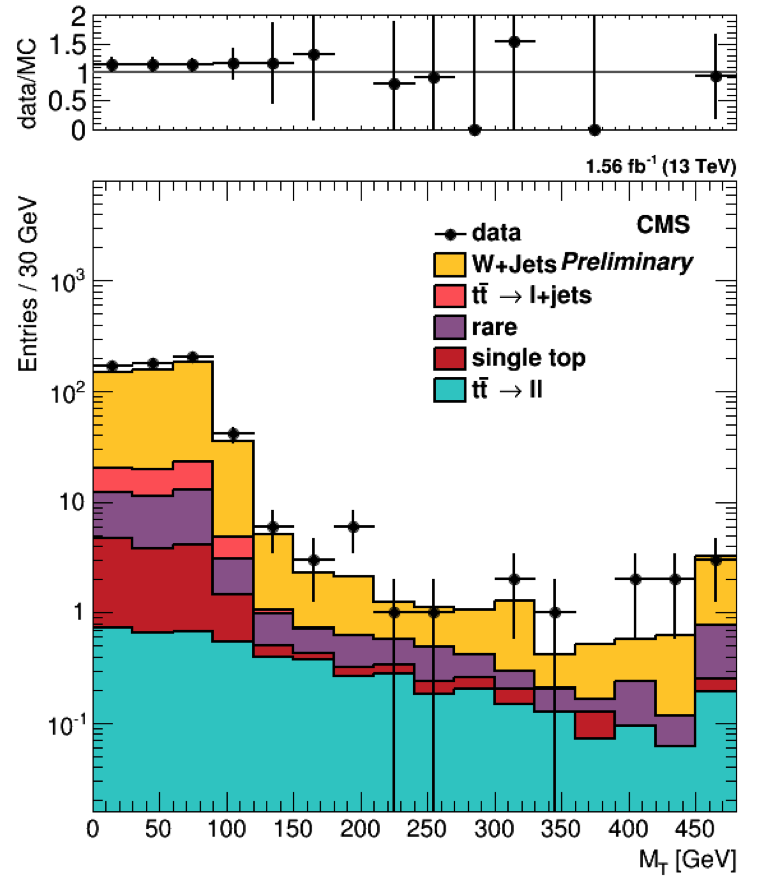
\includegraphics[width=0.44\textwidth]{Figures/bkg1lep/MTDist_3jets.png}
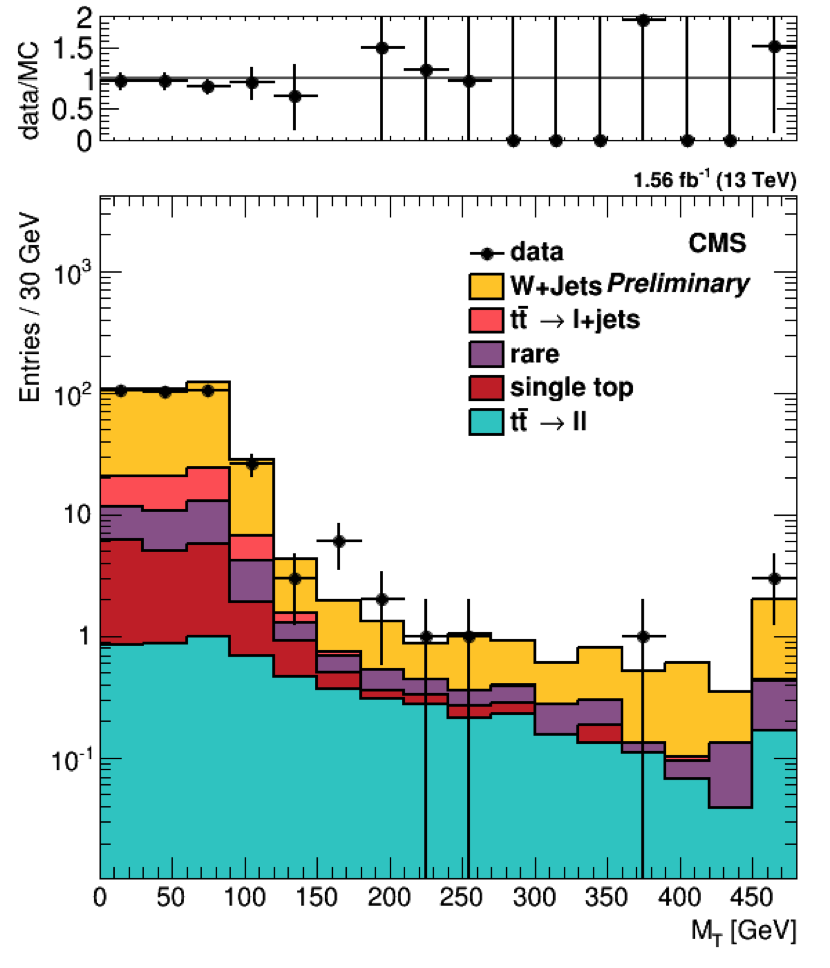
\includegraphics[width=0.44\textwidth]{Figures/bkg1lep/MTDist_4jets.png}
\caption{\label{fig:MT} Distribution of \MT for 3 and $\ge$ 4 jets 0b CRs.}
\end{figure}

The full MT distribution for the 0-btag CR is shown on Figure~\ref{fig:MT}.  There is good agreement between data and MC in both the peak region 
and the tail of the MT spectrum.  For the W+Jets, only the MT$>150$ \GeV region is used, to coincide with the requirement in the signal regions.  
The summary of yields for the CRs is shown on Table~\ref{tab:0b_CR:yields}.  All other 1-lepton background not from top decays will also be 
included in this estimate.  
%
As can be seen from Table~\ref{tab:0b_CR:yields},
there is close to 30\% contamination from dilepton and Z$\rightarrow\nu\nu$ backgrounds in these W+Jets CRs that needs to be subtracted.  
A 50$\%$ systematic uncertainty is assigned to this subtraction when calculating the  $N^{data,WJets}_{CR,0-btag}$.  

\begin{table}
\begin{center}
\small
\caption{\label{tab:0b_CR:yields} high $\Delta$M, 0b CR}
\resizebox{\textwidth}{!}{\begin{tabular}{|c|c|c|}\hline
  &==3 jets  & $\ge$ 4 jets  \\
 &MET $>$ 250&MET $>$ 250\\
\hline
1lep (not from top) $\pm \sigma^{MC}_{stat} $& 16.16$\pm$1.28 & 11.20$\pm$0.87\\
1lep (from top)$ \pm \sigma^{MC}_{stat} \pm \sigma^{MC}_{50\%syst} $& 0.08$\pm$0.03$\pm$0.04 & 0.39$\pm$0.08$\pm$0.19\\
$\ge$ 2lep (lost lep) $ \pm \sigma^{MC}_{stat} \pm \sigma^{MC}_{50\%syst} $  & 4.23$\pm$0.63$\pm$1.39 & 3.53$\pm$0.23$\pm$1.46\\
Z$\rightarrow\nu\nu  \pm \sigma^{MC}_{stat} \pm \sigma^{MC}_{50\%syst} $  & 3.74$\pm$0.15$\pm$1.69 & 1.99$\pm$0.11$\pm$0.84\\
Total BGs $ \pm \sigma^{MC}_{stat} \pm \sigma^{NonWJets MC}_{50\%syst} $ & 24.20$\pm$1.44$\pm$2.18 & 17.11$\pm$0.91$\pm$1.69\\
\hline
Data $\pm \sigma^{Data}_{stat}$ & 24.00$\pm$4.90 & 18.00$\pm$4.24\\
\hline
Data/MC  $\pm \sigma_{stat} \pm \sigma_{sys}$& 0.99$\pm$0.21$\pm$0.09 & 1.05$\pm$0.25$\pm$0.10\\
\hline
WJets purity $\pm \sigma_{stat} \pm \sigma_{sys}$ & 0.67$\pm$0.07$\pm$0.06 & 0.65$\pm$0.06$\pm$0.06\\
&&\\
N$^{data,WJets}_{0bCR}$: (1lep not from top) &15.96$\pm$4.90$\pm$0.65$\pm$2.19 & 12.09$\pm$4.24$\pm$0.27$\pm$1.70\\
&&\\
$\pm \sigma^{data}_{stat} \pm \sigma^{MC}_{stat} \pm \sigma^{MC}_{50\% syst}$&&\\\hline
\end{tabular}}
\end{center}
\end{table}

The final WJets estimates are shown in Table~\ref{tab:WJetsEstimate}.
\begin{table}
\begin{center}
\caption{\label{tab:WJetsEstimate}Values used for WJets Estimate with BTag SFs applied}
\resizebox{\textwidth}{!}{\begin{tabular}{|c|c|ccc|}\hline
\hline
  &==3 jets  && $\ge$ 4 jets &\\
 &MET $>$ 250& & MET $>$ 250&\\
 \hline
&&&&\\
N$^{data,WJets}_{0bCR2}$: (1lep not from top) &15.96 & & 12.09&\\
&&&&\\
$\pm \sigma^{data}_{stat} \pm \sigma^{MC}_{stat} \pm \sigma^{MC}_{50\% syst}$&$\pm$4.90$\pm$0.65$\pm$2.19&&$\pm$4.24$\pm$0.27$\pm$1.70&\\
\hline
&&&&\\
\hline
 &==3 jets  & $\ge$ 4 jets &$\ge$ 4 jets & $\ge$ 4 jets\\
 &MET $>$ 350&250 $<$ MET $<$ 350&350 $<$ MET $<$ 450&MET $>$ 450\\
 \hline
 &&&&\\
TF$_{MET}\pm \sigma^{MC}_{stat} $ & 0.37 $\pm$ 0.049 & 0.55 $\pm$ 0.073 & 0.25 $\pm$ 0.045 & 0.20 $\pm$ 0.033\\
&&&&\\
\hline
&&&&\\
TF$_{btags} \pm \sigma^{MC}_{stat}$& 0.18 $\pm$ 0.074 & 0.15 $\pm$ 0.032 & 0.29 $\pm$ 0.10 & 0.40 $\pm$ 0.19\\
&&&&\\
\hline
&&&&\\
WJets in SR & 1.06 & 0.96  & 0.86 & 0.98 \\
$\pm \sigma^{data}_{stat} \pm \sigma^{MC}_{stat} \pm \sigma^{MC}_{50\% syst}$  & $\pm$ 0.32 $\pm$ 0.43 $\pm$ 0.14 &  $\pm$ 0.34 $\pm$ 0.201 $\pm$ 0.13 &  $\pm$ 0.30 $\pm$ 0.28 $\pm$ 0.12 & $\pm$ 0.34 $\pm$ 0.45 $\pm$ 0.14 \\
&&&&\\
\hline
\end{tabular}}
\end{center}
\end{table}


\subsubsection{Systematic Uncertainties}
\label{subsec:bkg1l:sys}
The non-negligible systematic uncertainties affecting this background estimation are:
\begin{itemize}
  \item Data and MC statisitics - the largest uncertainty in the estimation is from the statistical uncertainty of the observed data yields in the CRs.
  \item W+b cross section - as we extrapolate in b-tagging using MC, we allow for a 50\% variation in the  W+b(b-bar) cross section.
  \item bTagging effiency and mistag rate - using SFs provided by the BTV POG.  Estimated by event reweighting using scale factors and MC b-tagging efficiencies %(Method 1a: https://twiki.cern.ch/twiki/bin/viewauth/CMS/BTagSFMethods#1a_Event_reweighting_using_scale)
  \item PDF - account for NNPDF3.0LO PDF variations.  Uncertainty is the standard deviatio of the average PDF variation.
  \item $Q^{2}$ - the largest two variations in renormalization and factorization scale,  $[\mu_{R}=2, \mu_{F}=2]  and [\mu_{R}=0.5, \mu_{F}=0.5]$,are considered 
  \item JES - the jet energy scale is varied, to account for diffences in jet acceptance. %as well as its effects on the calculation of t1 pfmet
  \item \MET resolution - a dedicated study described in Section~\ref{subsec:bkg1l:metResWithPhotons} is used to estimate uncertainties 
due to ``bin migration'' due to differences in the detailed shape of the \MET resolution function between data and MC. 
\end{itemize}
Table ~\ref{tab:1lepsysbtag} summarize the systematic uncertainties on the b-tag TF used to obtain the yield for each of the Signal Regions.  Table ~\ref{tab:1lepsys} shows the same for the \MET TF used to extrapolate in \MET.
\begin{table}
\begin{center}
\caption{\label{tab:1lepsysbtag}Systematic uncertainty on the b-tag TF}
\resizebox{\textwidth}{!}{\begin{tabular}{|c|c|ccc|}\hline
\hline
 &==3 jets  & $\ge$ 4 jets &$\ge$ 4 jets & $\ge$ 4 jets\\
 &MET $>$ 350&250 $<$ MET $<$ 350&350 $<$ MET $<$ 450&MET $>$ 450\\ 
\hline
Data Statistics&30$\%$&35$\%$&35$\%$&35$\%$\\
MC Statistics&41$\%$& 21 $\%$&32 $\%$&47.5$\%$\\
W+b xsec& 11$\%$ & 1$\%$ & 6$\%$ &7$\%$ \\
bTagging effiency and mistag rate&12$\%$ & 11$\%$ & 12$\%$ &12$\%$ \\
PDF&3$\%$ & 1$\%$ & 2$\%$ &5$\%$ \\
$Q^{2}$ &2$\%$ & 4.5$\%$ & 3$\%$ &4$\%$ \\
JES&11$\%$ & 11$\%$ & 5$\%$ &10$\%$ \\
Contamination in CR &14$\%$ &14$\%$ &14$\%$ & 14$\%$ \\
\hline
\end{tabular}}
\end{center}
\end{table}

\begin{table}
\begin{center}
\caption{\label{tab:1lepsys}Systematic uncertainty on the \MET TF}
\resizebox{\textwidth}{!}{\begin{tabular}{|c|c|ccc|}\hline
\hline
 &==3 jets  & $\ge$ 4 jets &$\ge$ 4 jets & $\ge$ 4 jets\\
 &MET $>$ 350&250 $<$ MET $<$ 350&350 $<$ MET $<$ 450&MET $>$ 450\\ 
\hline
MC Statistics&13$\%$&13$\%$&18$\%$&17$\%$\\
W+b xsec&1.4$\%$&0.3$\%$&0.4$\%$&0.4$\%$\\
bTagging effiency and mistag rate&1.$\%$&1.$\%$&1.$\%$&1.$\%$\\
PDF&1$\%$&1$\%$&1$\%$&1$\%$\\
$Q^{2}$ &2$\%$&1$\%$&1$\%$&1$\%$\\
JES&1$\%$&5$\%$&5$\%$&7$\%$\\
\MET resolution $\%$ & & & \\
\hline
\end{tabular}}
\end{center}
\end{table}

\subsubsection{Systematics due to differences in \MET resolution function between data and MC}
\label{subsec:bkg1l:metResWithPhotons}

{\bf fkw comment: here we describe HJ's study with photons}

\subsubsection{Summary of One Lepton background estimate}
\label{sec:bkg1l:summary}

{\bf fkw comment: we still need to add in the pieces that come from MC straight up, and add it to the data derived stuff.}


\subsection{\texorpdfstring{$\cPZ\to\cPgn\cPagn$}{Znunu} background}
\label{sec:bkgZnunu}

{\bf fkw comment: This section exists only in AN15-333 }


\section{Results}
\label{sec:yields}

\section{Summary of systematic uncertainties}
\label{sec:systematics}

\section{Statistical method for interpreting results}
\label{sec:statisticalMethod}

This section gives a description of the statistical methods used to interpret the results of section~\ref{sec:yields}.
The results are interpreted using expected exclusion limits and significance for the available benchmark points.

A binned likelihood fit is performed over analysis bins using the Higgs Combine tool~\cite{url:higgscombine}. 
For signal regions with a nonzero signal yield, the yield will be modified such that it is set to 10e-5.
A systematic uncertainty of 10\% is assumed for signal, based on the 8 TeV analysis, and is taken as correlated across all bins in the fit. 
{\color{red} CHECK THIS!}

The expected exclusion limits at the 95\% CL are calculated using asymptotic \CLs (with a-priori expected background)~\cite{Cowan:2010js}:
{\small
\begin{verbatim}
combine -M Asymptotic datacard.txt --noFitAsimov -n stringForRootfileOutput
\end{verbatim}
}

Expected significances are calculated using a profile likelihood scan (with a-priori expected background):
{\footnotesize
\begin{verbatim}
combine -M ProfileLikelihood --significance datacard.txt -t 400 --expectSignal=1 -n stringForRootfileOutput
\end{verbatim}
}
The string shows the command using 400 toys in the scan.


\section{Interpretation of results}
\label{sec:interpretation}

This section contains the interpretation of the results of section~\ref{sec:yields} based on the methods of section~\ref{sec:statisticalMethod}.

Table~%\ref{XXX} 
shows the 95\% CL expected exclusion limits for few benchmark model.
{\color{red} ADD TABLE XXX.}

Table~%\ref{YYY} 
shows the expected significances for the same benchmark model.
{\color{red} ADD TABLE YYY.}


{\color{red} Maybe add a small discussion.}


\section{Conclusions}
\label{sec:conclusions}

\clearpage
\appendix

\section{Data versus simulation comparison}
\label{sec:dataVsMC}

\section{Trigger efficiencies}
\label{sec:triggerEff}

\section{Signal variable studies for T2tt like signatures}
\label{sec:sigvarstudy}

This appendix discusses investigations on various variables suitable for signal discriminating variables. As signal we have four mass points of top squark pair production where both top squark decays are $\PSQt\to\cPqt\PSGczDo$.

The distributions on those variables are investigated, and relative sensitivity values are given for ad-hoc chosen selection criteria.
Although not chosen, some of these variables might still be useful in a later iteration of this analysis when either more data will be available or these variables are less correlated to current signal variable and such could be chosen by a multivariate classifier.

This study has been performed before the final event selection had been decided. Therefore, the yields will not match those of the analysis described above. However, the relative yields for the signal regions defined in this section should be largely unaffected by the differences in the event selection.

Another difference for this section is that the simulation had been normalized to 5 or 10\fbinv.

\subsection{Event selection for this study, signal mass points}
\label{sec:sigvarstudy:evtselection}

\begin{itemize}
\item First vertex is good.
\item Exactly one selection lepton:
	\begin{itemize}
	\item Electrons: $\pt>40\GeV$, $|\eta|<2.1$, medium ID, miniiso$ < 0.1$,
	\item Muons: $\pt>30\GeV$, $|\eta|<2.1$, medium ID, miniiso$ < 0.2$,
	\end{itemize}
\item No additional veto lepton:
	\begin{itemize}
	\item Electrons: $\pt>10\GeV$, $|\eta|<2.4$, veto ID, miniiso$ < 0.2$,
	\item Muons: $\pt>10\GeV$, $|\eta|<2.4$, loose ID, miniiso$ < 0.2$,
	\end{itemize}
\item  At least four jets ($\pt>30\GeV$, $|\eta|<2.4$, loose ID),
\item  At least on b-jet (medium CSVv2+IVF WP),
\item  $\MET>200\GeV$ (type-1 corrected),
\item  $\MT>150\GeV$,
\item  $\minDPhiMETjet>0.8$.
\end{itemize}
In addition, four selection stages were investigated:
\begin{enumerate}
\item Preselection as above,
\item Preselection plus $\MET>300\GeV$,
\item Preselection plus $\MET>300\GeV$, $\chi^2_{\mathrm{had.}\cPqt}<10$,
\item Preselection plus $\MET>300\GeV$, $\chi^2_{\mathrm{had.}\cPqt}<10$, $\MTtW>200\GeV$.
\end{enumerate}
The $\chi^2_\mathrm{had.top}$ variable was calculated similar to the 8\TeV analysis~\cite{Chatrchyan:2013xna}, however with a flat jet energy resolution of 10\%.

For this study, PHYS14 simulation was used. The signal mass points are:
\begin{itemize}
\item $M_{\PSQt} = 425\GeV$, $M_{\PSGczDo} = 325\GeV$,
\item $M_{\PSQt} = 500\GeV$, $M_{\PSGczDo} = 325\GeV$,
\item $M_{\PSQt} = 650\GeV$, $M_{\PSGczDo} = 325\GeV$,
\item $M_{\PSQt} = 850\GeV$, $M_{\PSGczDo} = 100\GeV$.
\end{itemize}

\subsection{Signal variables under study}
\label{sec:sigvarstudy:variables}

\subsubsection{\MTtW}

The \MTtW variable~\cite{Bai:2012gs} is defined as
\begin{align}
\MTt^W = &\min\left\{m_y\text{ consistent with } \left[ p_1^2 = 0, \right.\right. 
(p_1+p_\ell)^2 = p_2^2 = M_{\PW}, \\
& \ptvec^1+\ptvec^2 = \VEtmiss, 
\left.\left. (p_1+p_\ell+p_{\cPqb_1})^2=(p_2+p_{\cPqb_2})^2 = m_y^2,\right]\right\} \nonumber
\end{align}
The basic idea is to try to split \MET into its components due to the lost \PW boson and $\cPgn_1$, such that you get two symmetric masses consistent with event kinematics of a lost lepton in $\cPqt\cPaqt$.
The output is the fitted mass $m_y$.
Therefore, the variable is specifically designed to reduce dileptonic $\cPqt\cPaqt$ with a lost lepton for a single-lepton top squark search, for which $m_y \approx M_{\cPqt}$.

For further details, please see also section {\color{red} REFERENCE SECTION ABOVE}.

Figure~\ref{fig:sigvarstudy:MT2WTopness:MT2W} shows the \MTtW distribution after preselection plus $\MET>300\GeV$. As a test selection $\MTtW>200\GeV$ was chosen.

\begin{figure}
\subfigure[\MTtW distribution.]{
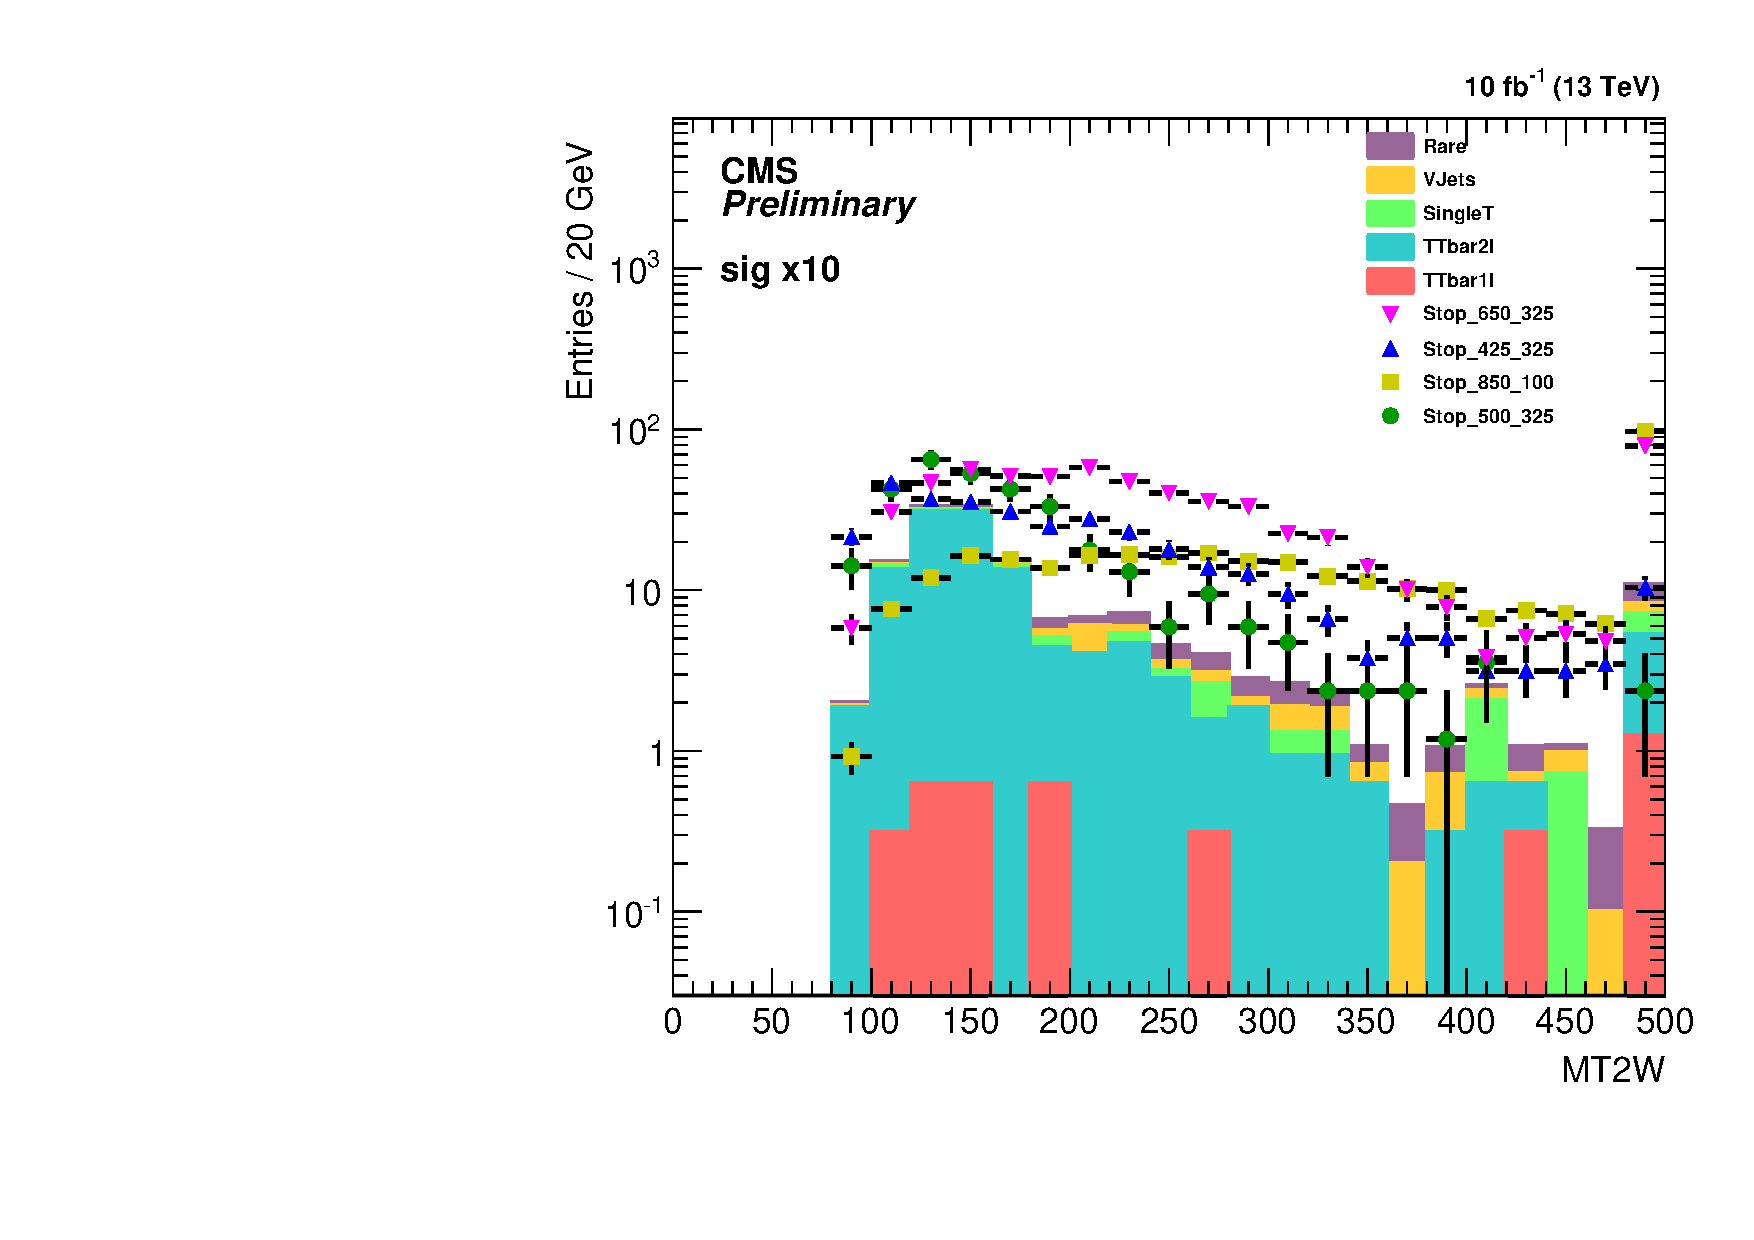
\includegraphics[width=0.49\textwidth]{Figures/SignalVariableStudies/MT2W.pdf}
\label{fig:sigvarstudy:MT2WTopness:MT2W}
}
\subfigure[Topness distribution.]{
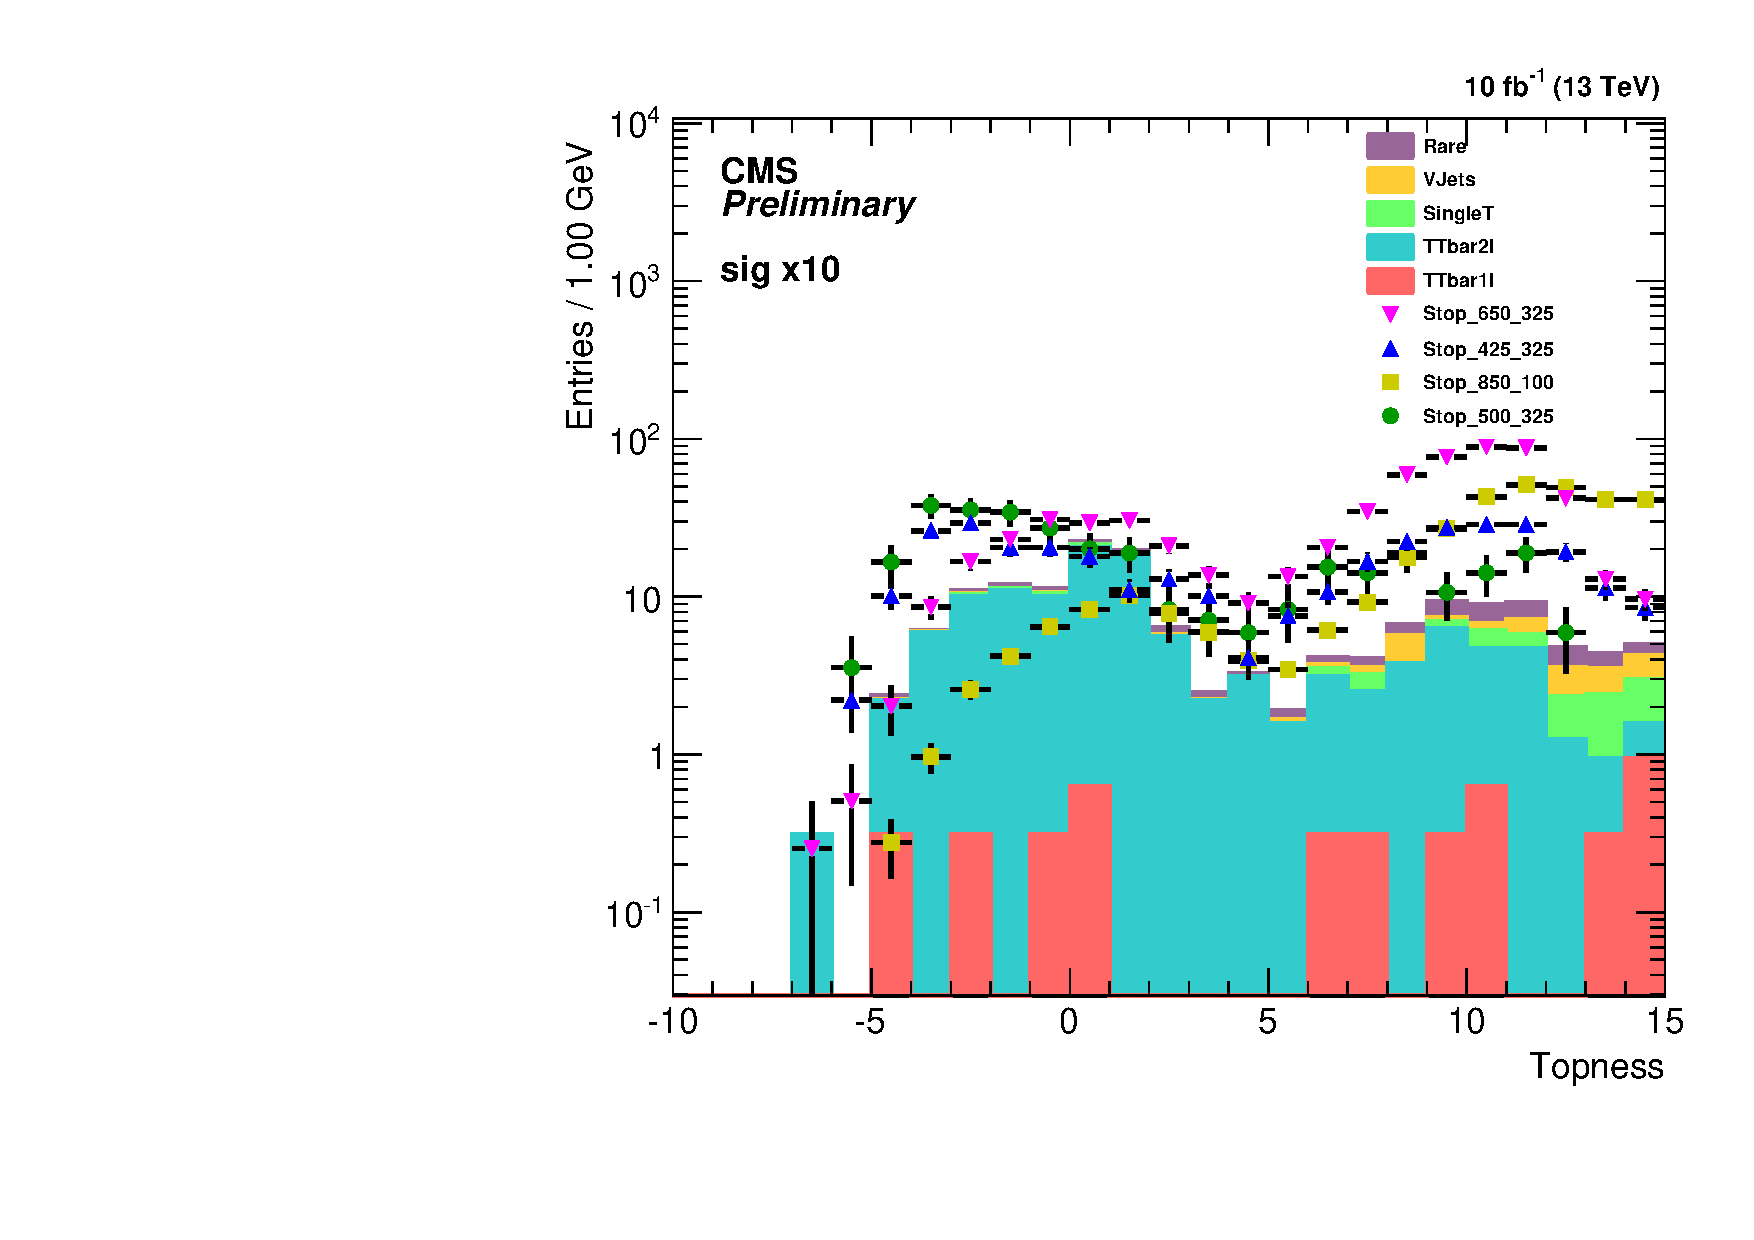
\includegraphics[width=0.49\textwidth]{Figures/SignalVariableStudies/Topness.pdf}
\label{fig:sigvarstudy:MT2WTopness:Topness}
}
\caption{\label{fig:sigvarstudy:MT2WTopness} The \MTtW (left) and topness (right) distributions.}
\end{figure}

\subsubsection{Topness}
\label{sec:sigvarstudy:topness}

The topness variable~\cite{Graesser:2012qy} is defined as
\begin{align} t = &\ln(\min S)~\text{ with }~ S(\vec{p}_\PW, p_{\cPgn,z}) = \\
 &\frac{(M_\PW^2-(p_\cPgn+p_\ell)^2)^2}{a_\PW^4} + \frac{(M_\cPqt^2-(p_{\cPqb_1}+p_\ell+p_\cPgn)^2)^2}{a_\cPqt^4}
 + \frac{(M_\cPqt^2 - (p_{\cPqb_2}+p_\PW)^2)^2}{a_t^4} + \frac{(4M_\cPqt^2-(\sum p_i)^2)^2}{a_\mathrm{CM}^4}. \nonumber
 \end{align}
Here, the $a$ terms are resolution terms with values $a_\PW = 5\GeV$, $a_\cPqt = 15\GeV$, $a_\mathrm{CM} = 1\TeV$.
Thus, the topness variable uses a similar idea as for \MTtW, but including the top quark mass requirement, and resolution terms $a$.

The selection of two b jets is done the same as for the \MTtW variable.

Figure~\ref{fig:sigvarstudy:MT2WTopness:Topness} shows the topness distribution after preselection plus $\MET>300\GeV$. As a test selection $t>9$ was chosen.


\subsubsection{Modified topness}
\label{sec:sigvarstudy:modtopness}

After studying the topness variable in great detail, it was found that two terms diminish the signal discriminator power at high values of the topness variable. Therefore a modification was introduced:
\begin{equation}
t_\mathrm{mod} = \ln(\min S)~\text{ with }~ S(\vec{p}_\PW, p_{\cPgn,z}) = \frac{(M_\PW^2-(p_\cPgn+p_\ell)^2)^2}{a_\PW^4} + \frac{(M_\cPqt^2 - (p_{\cPqb_2}+p_\PW)^2)^2}{a_\cPqt^4}.
\end{equation}
The top quark mass constraint for the top quark decay with the reconstructed lepton was dropped, as well as the center-of-mass constraint.

The reason is the following: The W boson mass constraint for the top quark decay with the reconstructed lepton already constraints the \MET splitting well enough. This can get diminished if the jet used in the corresponding top quark mass constraint does not come from the top quark decay (like mistagged jet or b-jet from gluon splitting). Dropping the center-of mass term has only a small effect.

Figure~\ref{fig:sigvarstudy:TopnessModMT2lbb:TopnessMod} shows the modified topness distribution after preselection plus $\MET>300\GeV$. As a test selection $t_\mathrm{mod}>7$ was chosen.

\begin{figure}
\subfigure[Modified topness distribution.]{
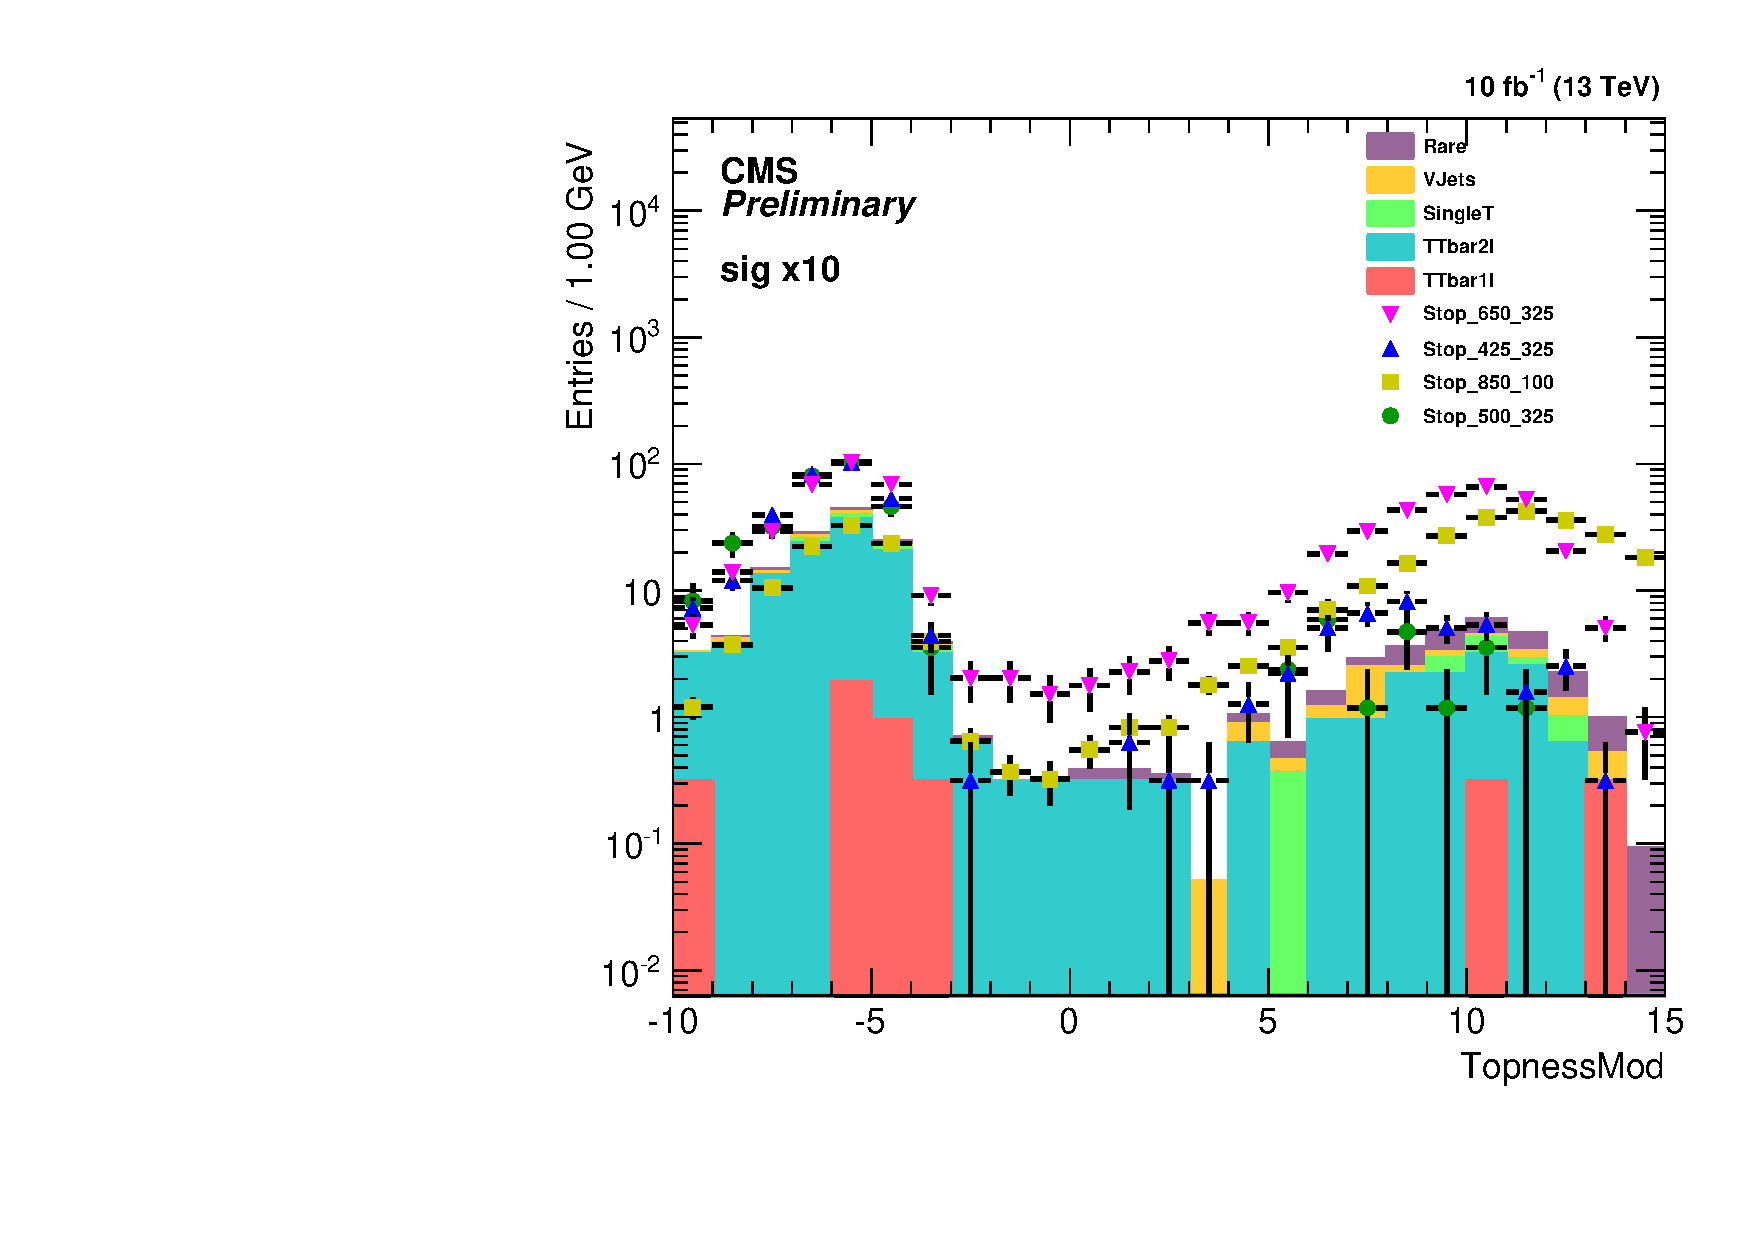
\includegraphics[width=0.49\textwidth]{Figures/SignalVariableStudies/TopnessMod.pdf}
\label{fig:sigvarstudy:TopnessModMT2lbb:TopnessMod}
}
\subfigure[$\MTt(\ell\cPqb,\cPqb)$ distribution.]{
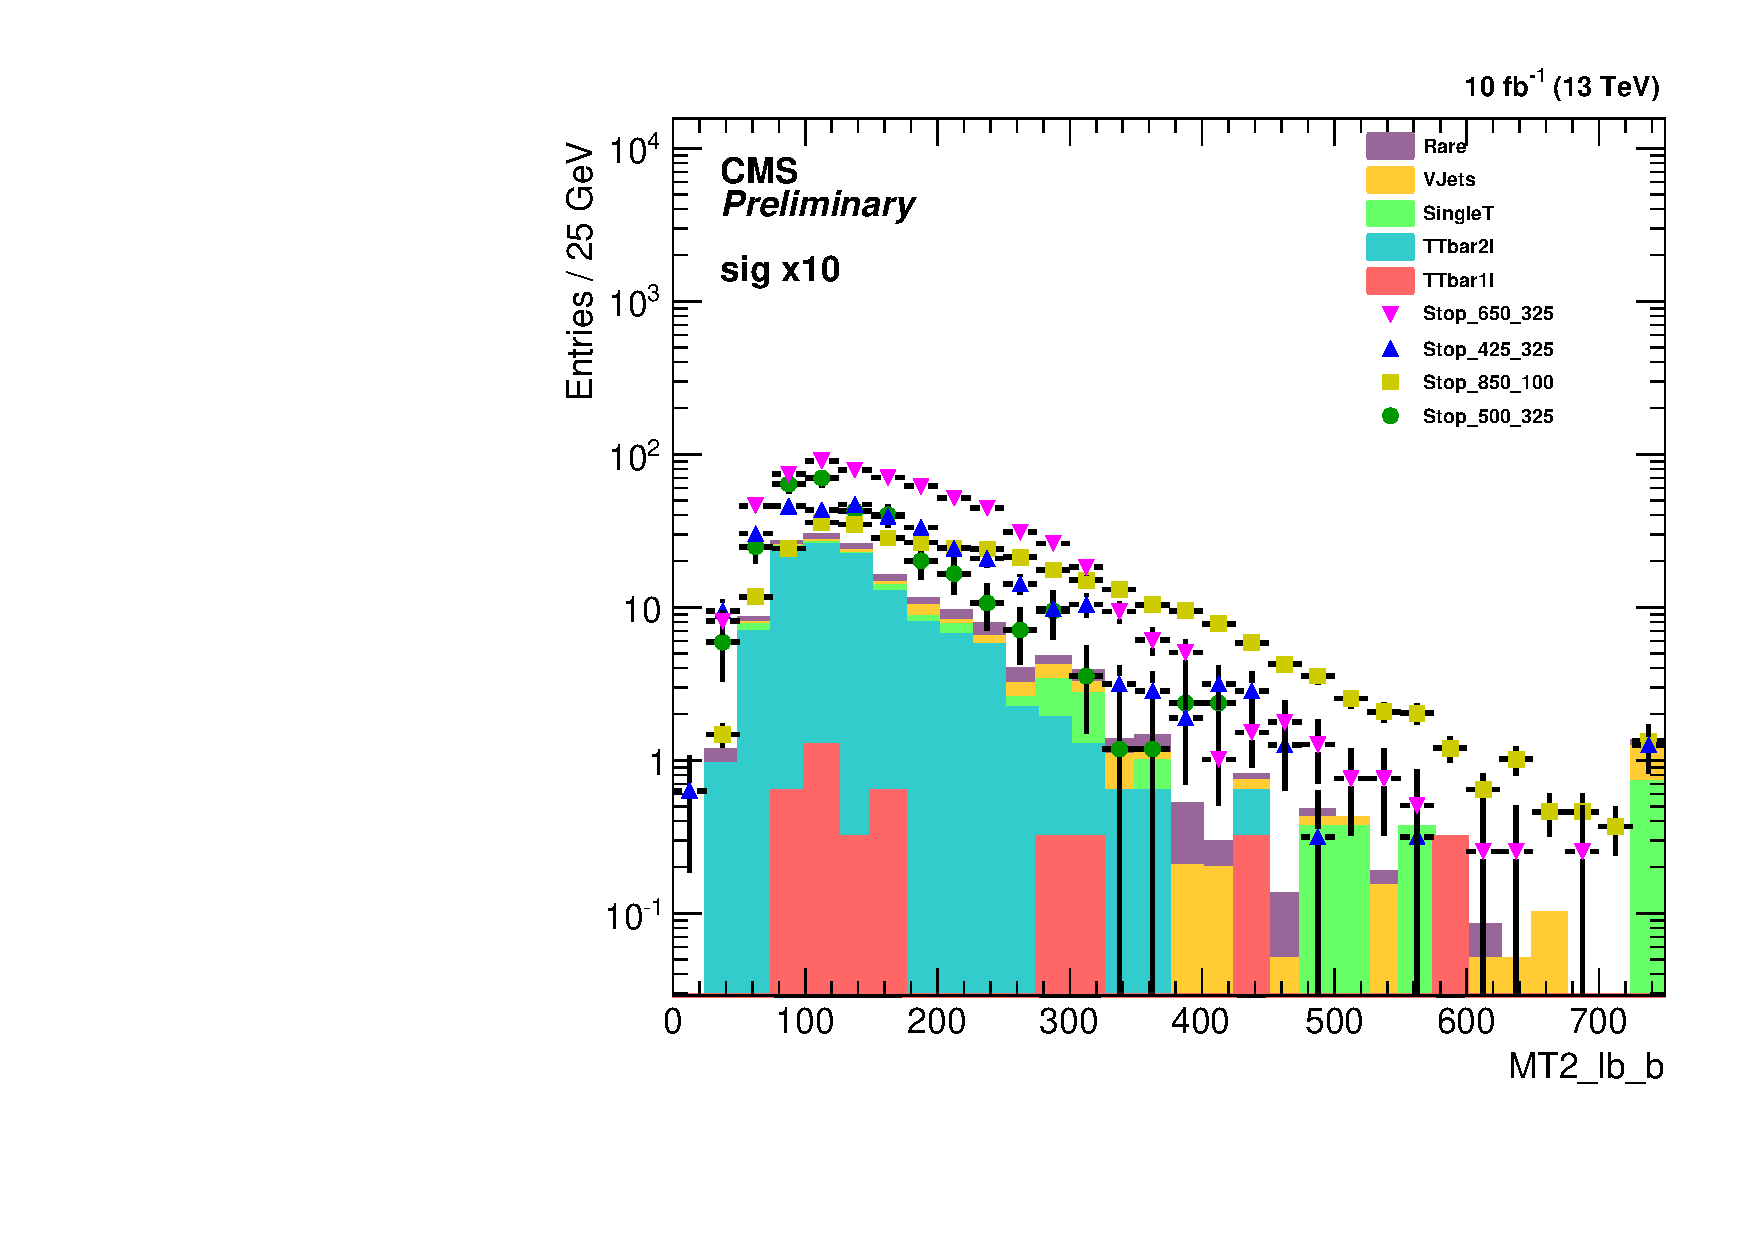
\includegraphics[width=0.49\textwidth]{Figures/SignalVariableStudies/MT2_lb_b.pdf}
\label{fig:sigvarstudy:TopnessModMT2lbb:MT2lbb}
}
\caption{\label{fig:sigvarstudy:TopnessModMT2lbb} The modified topness (left) and $\MTt(\ell\cPqb,\cPqb)$ (right) distributions.}
\end{figure}

\subsubsection{$\MTt(\ell\cPqb,\cPqb)$}

The \MTt variable~\cite{Lester:1999tx} is defined as 
\begin{equation}
 \MTt(M_{\tilde{\chi}}) = \min_{\scriptscriptstyle\ptvec^{\tilde{\chi}(1)} + \ptvec^{\tilde{\chi}(2)} = \VEtmiss} \left[ \max \left( \MT^{(1)} , \MT^{(2)} \right) \right].
\end{equation}
This variable was designed to measure mass of pair-produced particles, each decaying semi-invisible. As visible objects, we take here ($1\ell + 1\cPqb$) and ($1\cPqb$), and the testmass $M_{\tilde{\chi}} = 0$.
The selection of two b jets is done the same as for the \MTtW variable.

Figure~\ref{fig:sigvarstudy:TopnessModMT2lbb:MT2lbb} shows the $\MTt(\ell\cPqb,\cPqb)$ distribution after preselection plus $\MET>300\GeV$. As a test selection $\MTt(\ell\cPqb,\cPqb)>175\GeV$ was chosen.

\subsubsection{(Massless) $\MTt(\ell\cPqb,\cPqb\cPq\cPq)$}

We can also define the \MTt variable with two visible systems as ($1\ell + 1\cPqb$) and ($1\cPqb+2\cPq$). The assumption is to fully reconstruct the top squark pair production signature. While the choice of b jets is kept the same as in the previous sections, for the ``normal'' jets, we loop over all jet pair combinations, that do not include the selected b jets, and choose that combination that yields smallest $\MTt(\ell\cPqb,\cPqb\cPq\cPq)$.

When studying its distribution (see figure~\ref{fig:sigvarstudy:MT2lbbqq:massive}), we find no discrimination power. As found in an earlier search using the \MTt variable~\cite{Khachatryan:2015vra}, the mass term of the visible systems are the reason for this effect. As done in this search, after removing the visible object mass in the \MTt calculation, seen in figure~\ref{fig:sigvarstudy:MT2lbbqq:massless}, the signal discrimination is restored. However, the signal efficiency is also strongly reduced. For this (massless) variable, a test selection of $\MTt(\ell\cPqb,\cPqb\cPq\cPq)>175\GeV$ was chosen.


\begin{figure}
\subfigure[Massive $\MTt(\ell\cPqb,\cPqb\cPq\cPq)$ distribution.]{
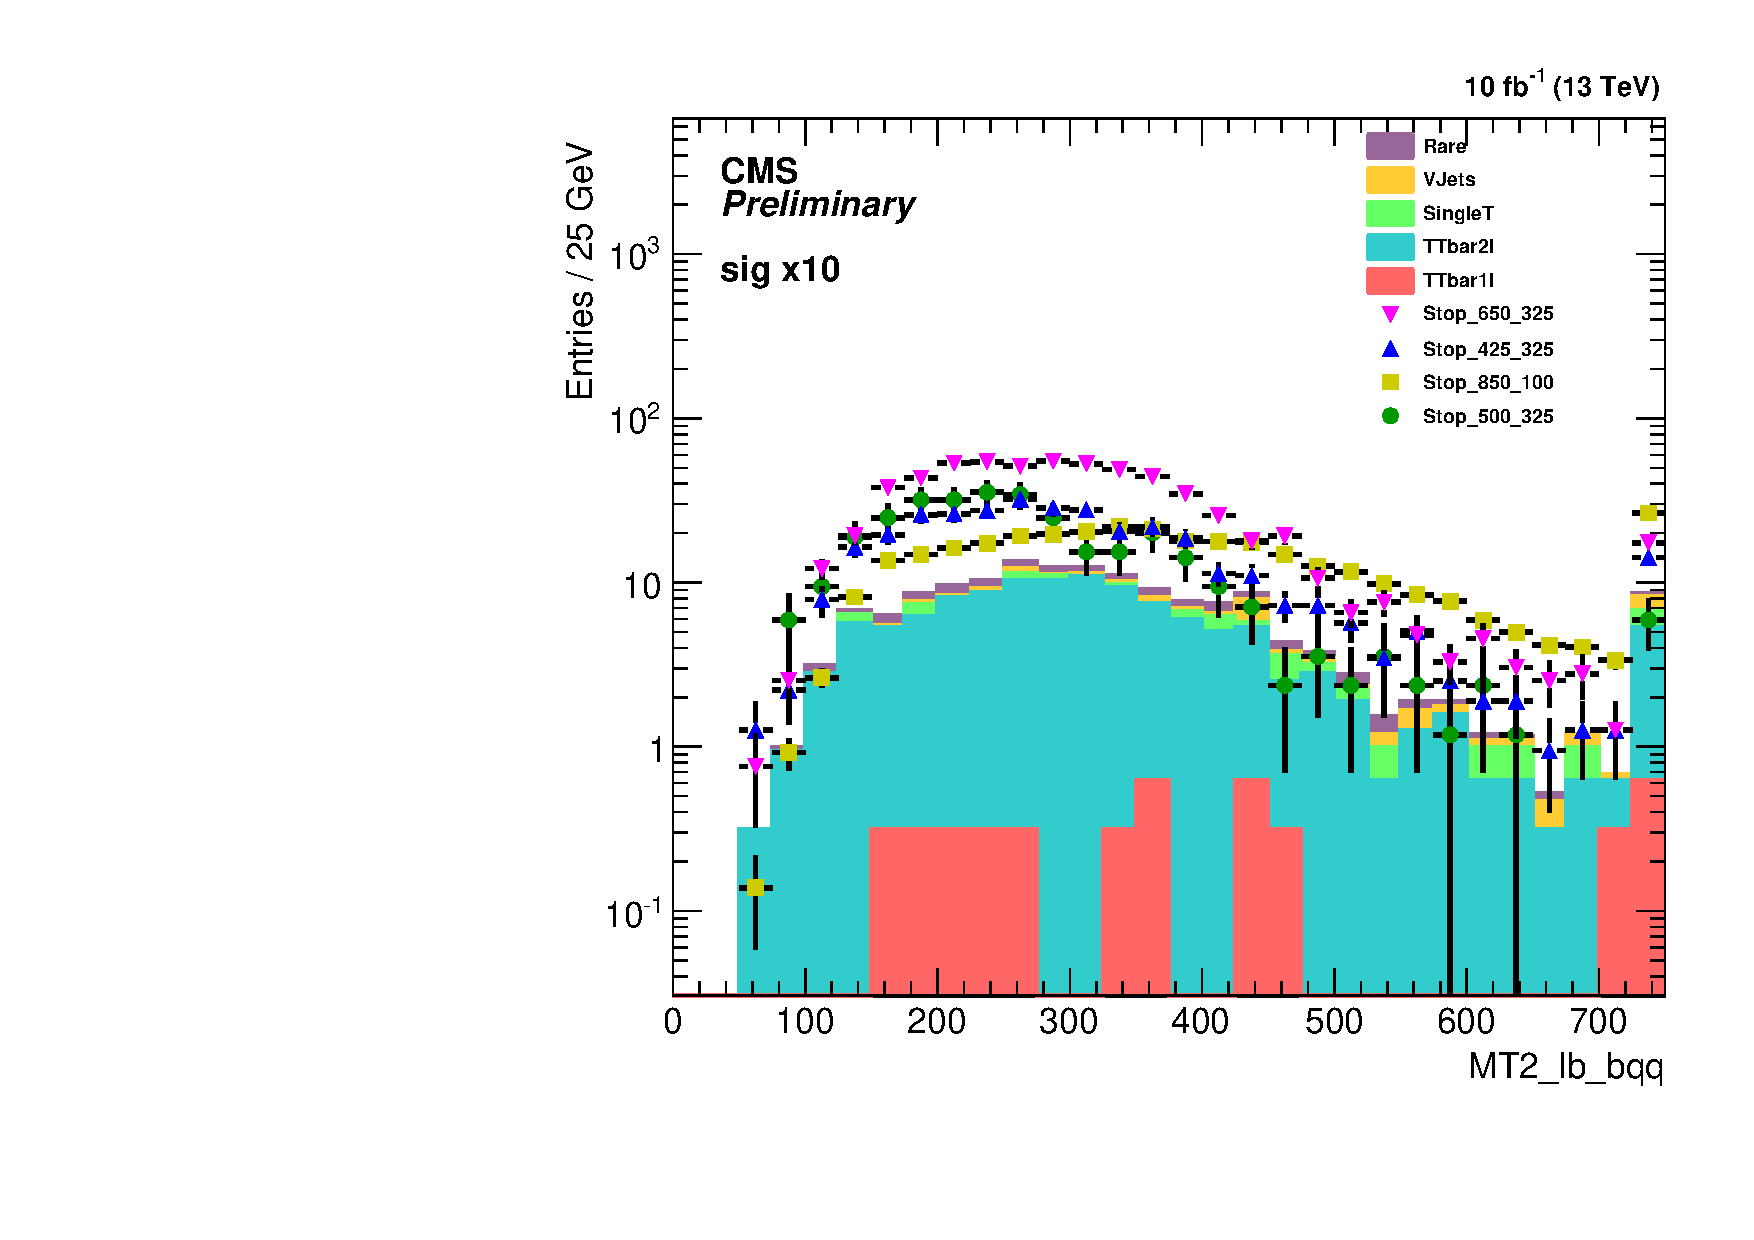
\includegraphics[width=0.49\textwidth]{Figures/SignalVariableStudies/MT2_lb_bqq.pdf}
\label{fig:sigvarstudy:MT2lbbqq:massive}
}
\subfigure[Massless $\MTt(\ell\cPqb,\cPqb\cPq\cPq)$ distribution.]{
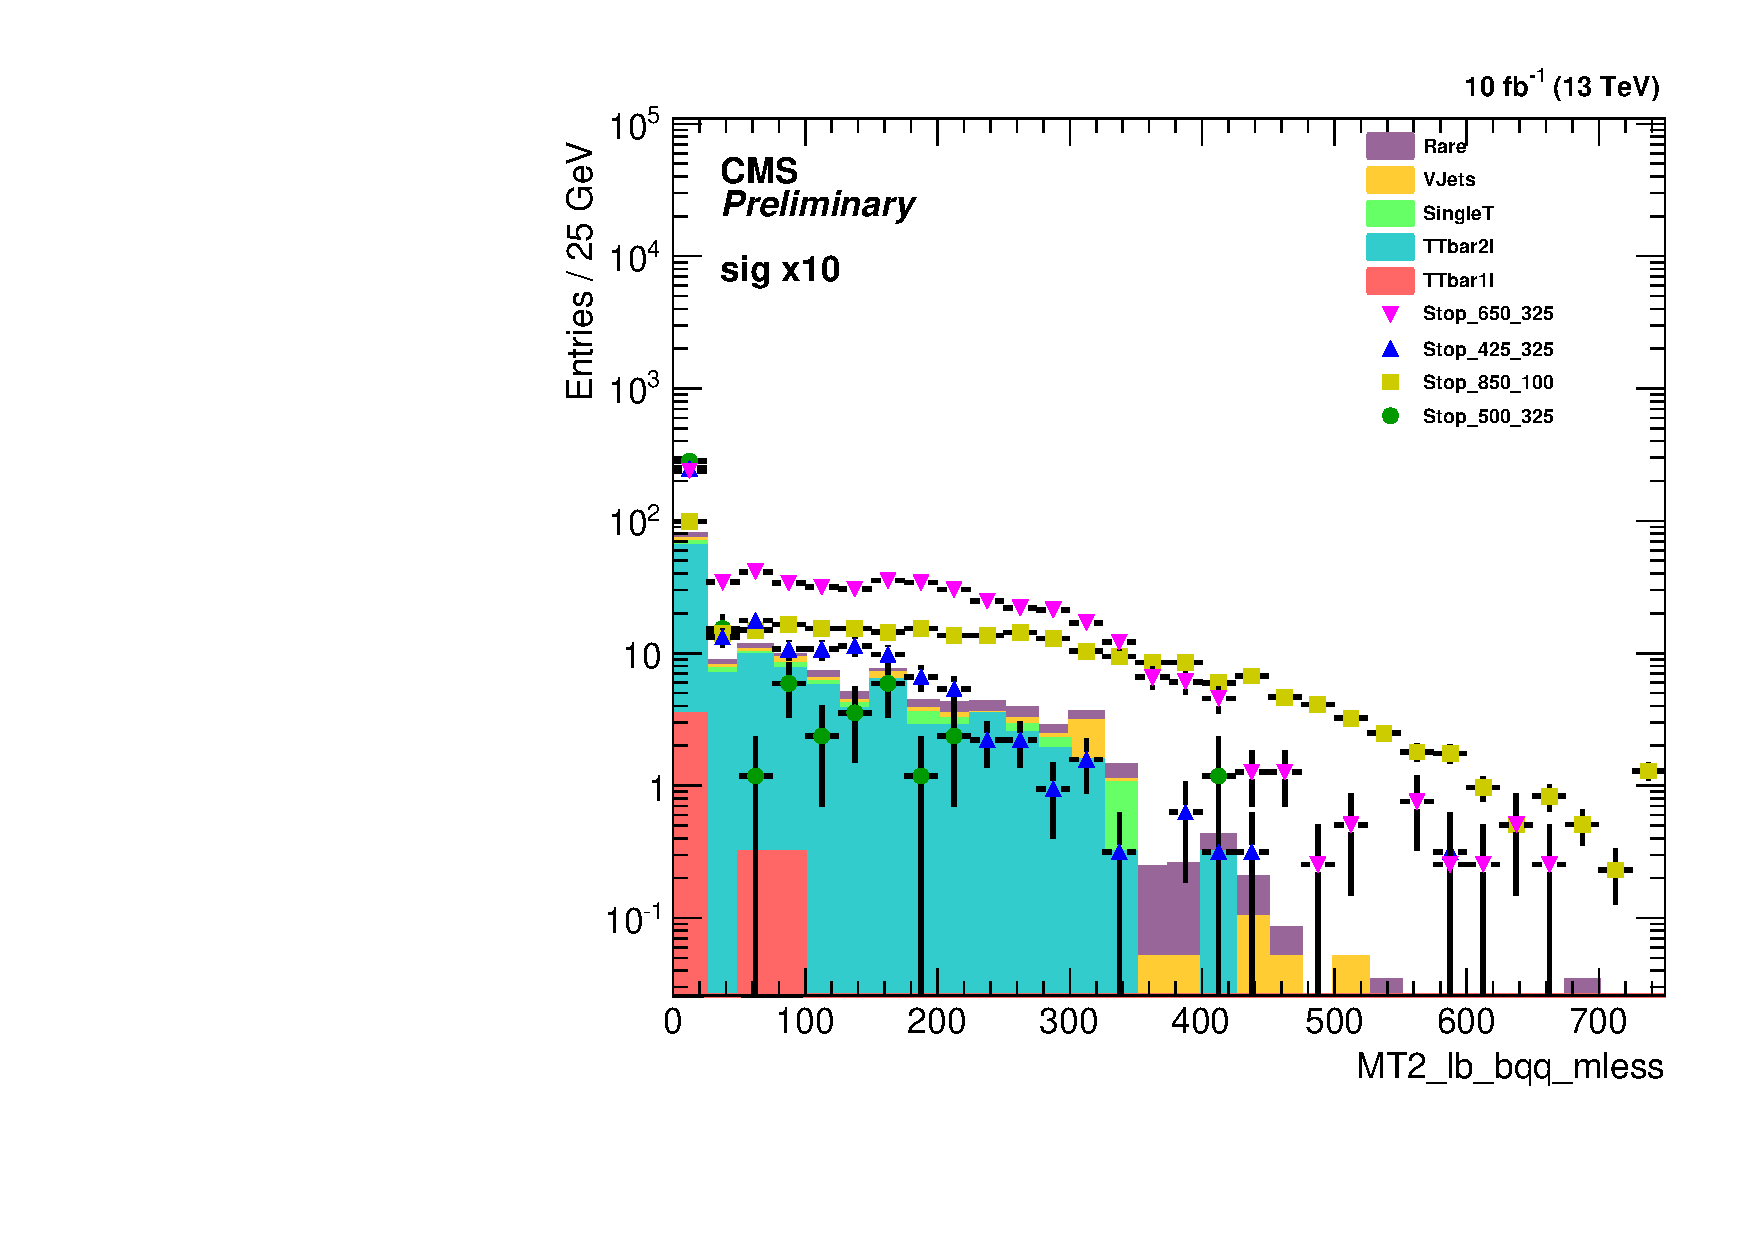
\includegraphics[width=0.49\textwidth]{Figures/SignalVariableStudies/MT2_lb_bqq_mless.pdf}
\label{fig:sigvarstudy:MT2lbbqq:massless}
}
\caption{\label{fig:sigvarstudy:MT2lbbqq} Massive (left) and massless (right) $\MTt(\ell\cPqb,\cPqb\cPq\cPq)$ distributions.}
\end{figure}

\subsubsection{(Massless) $\MTt(\ell,\cPq\cPq)$}

As it can be guessed, this variable is similar as in the section before, but without the requirements of the two b-jets. Such a variable could be sensitive for the production of charginos as in $\PSQt\to\cPqb\PSGcpmDo$, $\PSGcpmDo\to\PW\PSGczDo$.

Figure~\ref{fig:sigvarstudy:MT2lqq} shows the (massless) $\MTt(\ell,\cPq\cPq)$ distribution after preselection plus $\MET>300\GeV$. As a test selection $\MTt(\ell,\cPq\cPq)>50(60)\GeV$ was chosen.

\begin{figure}
\subfigure[Massive $\MTt(\ell,\cPq\cPq)$ distribution.]{
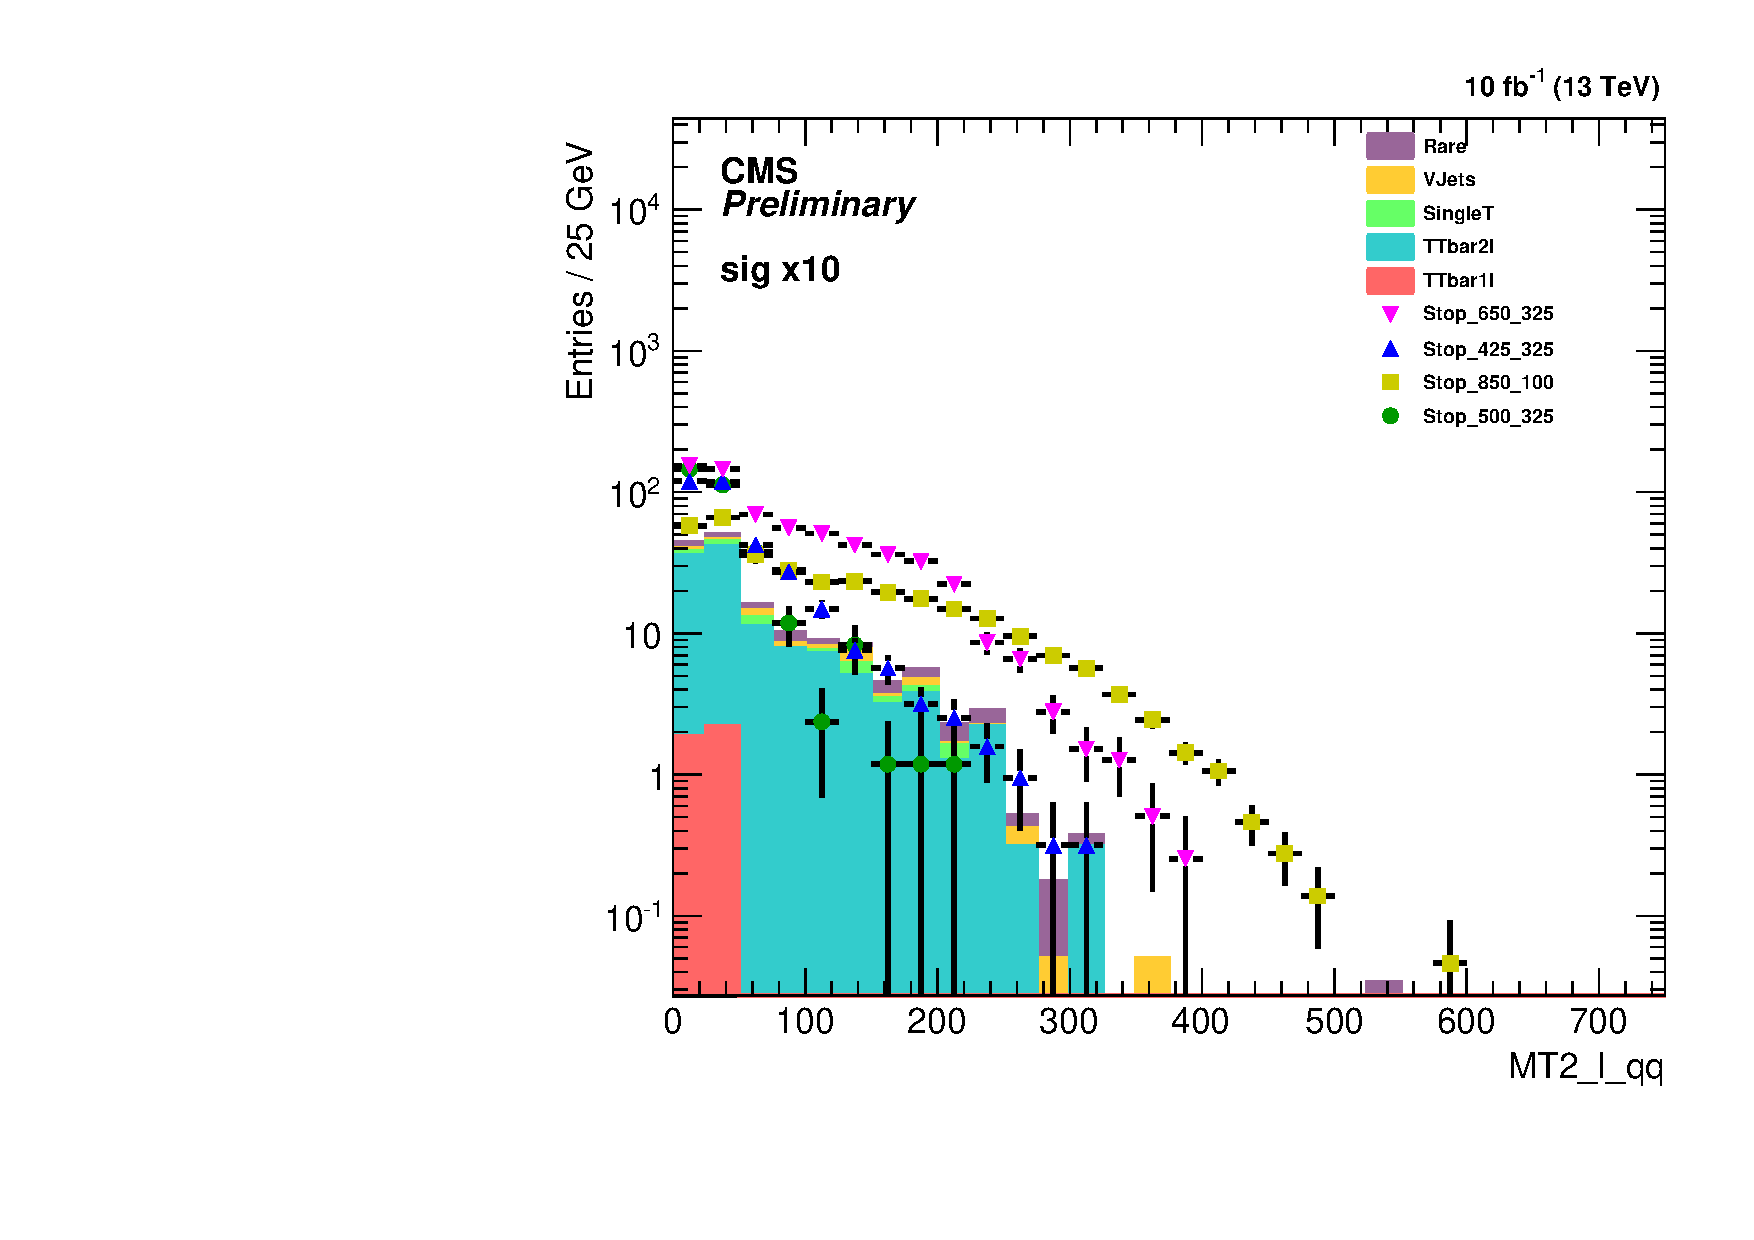
\includegraphics[width=0.49\textwidth]{Figures/SignalVariableStudies/MT2_l_qq.pdf}
\label{fig:sigvarstudy:MT2lqq:massive}
}
\subfigure[Massless $\MTt(\ell\cPqb,\cPqb\cPq\cPq)$ distribution.]{
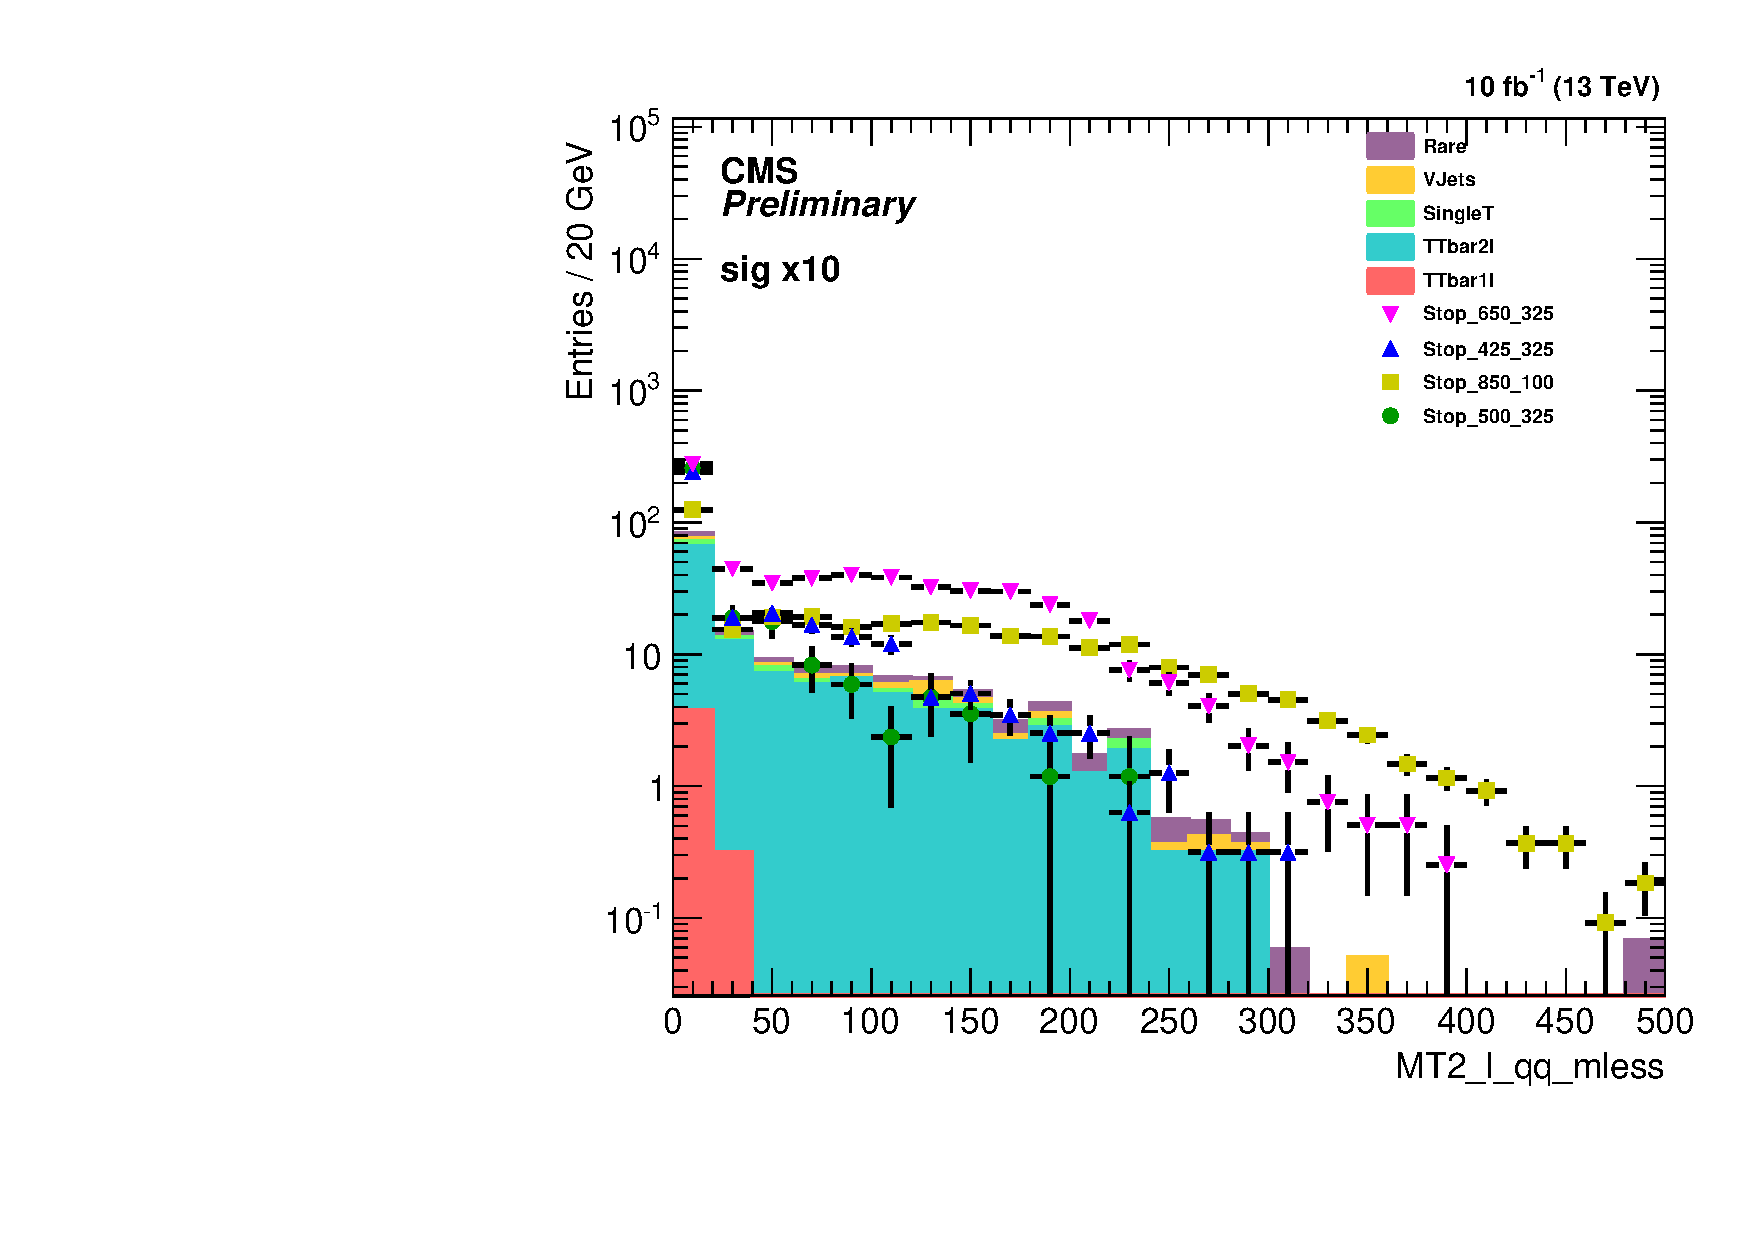
\includegraphics[width=0.49\textwidth]{Figures/SignalVariableStudies/MT2_l_qq_mless.pdf}
\label{fig:sigvarstudy:MT2lqq:massless}
}
\caption{\label{fig:sigvarstudy:MT2lqq} Massive (left) and massless (right) $\MTt(\ell,\cPq\cPq)$ distributions.}
\end{figure}

\subsubsection{$R_M$}
The $R_M$ variable~\cite{An:2015uwa} targets the compressed spectra signatures (small $\Delta M$ between the top squark and the LSP masses).
The variable is defined as 
\begin{equation}
R_M =  \frac{\MET}{\pt(j_1)} \approx \frac{\MET}{\pt(j_\mathrm{ISR})}.
\end{equation}
The idea is that the event is tagged via an ISR jet. Thus, for signal We expect a balance of \MET and the leading jet, while for SM background, lower values of $R_M$ are also possible.
For the leading jet, we require $\pt>300\GeV$.

Figure~\ref{fig:sigvarstudy:RMMTq:RM} shows the $R_M$ distribution after preselection plus $\MET>300\GeV$. As a test selection $R_M>0.8$ was chosen.

\begin{figure}
\subfigure[$R_M$ distribution.]{
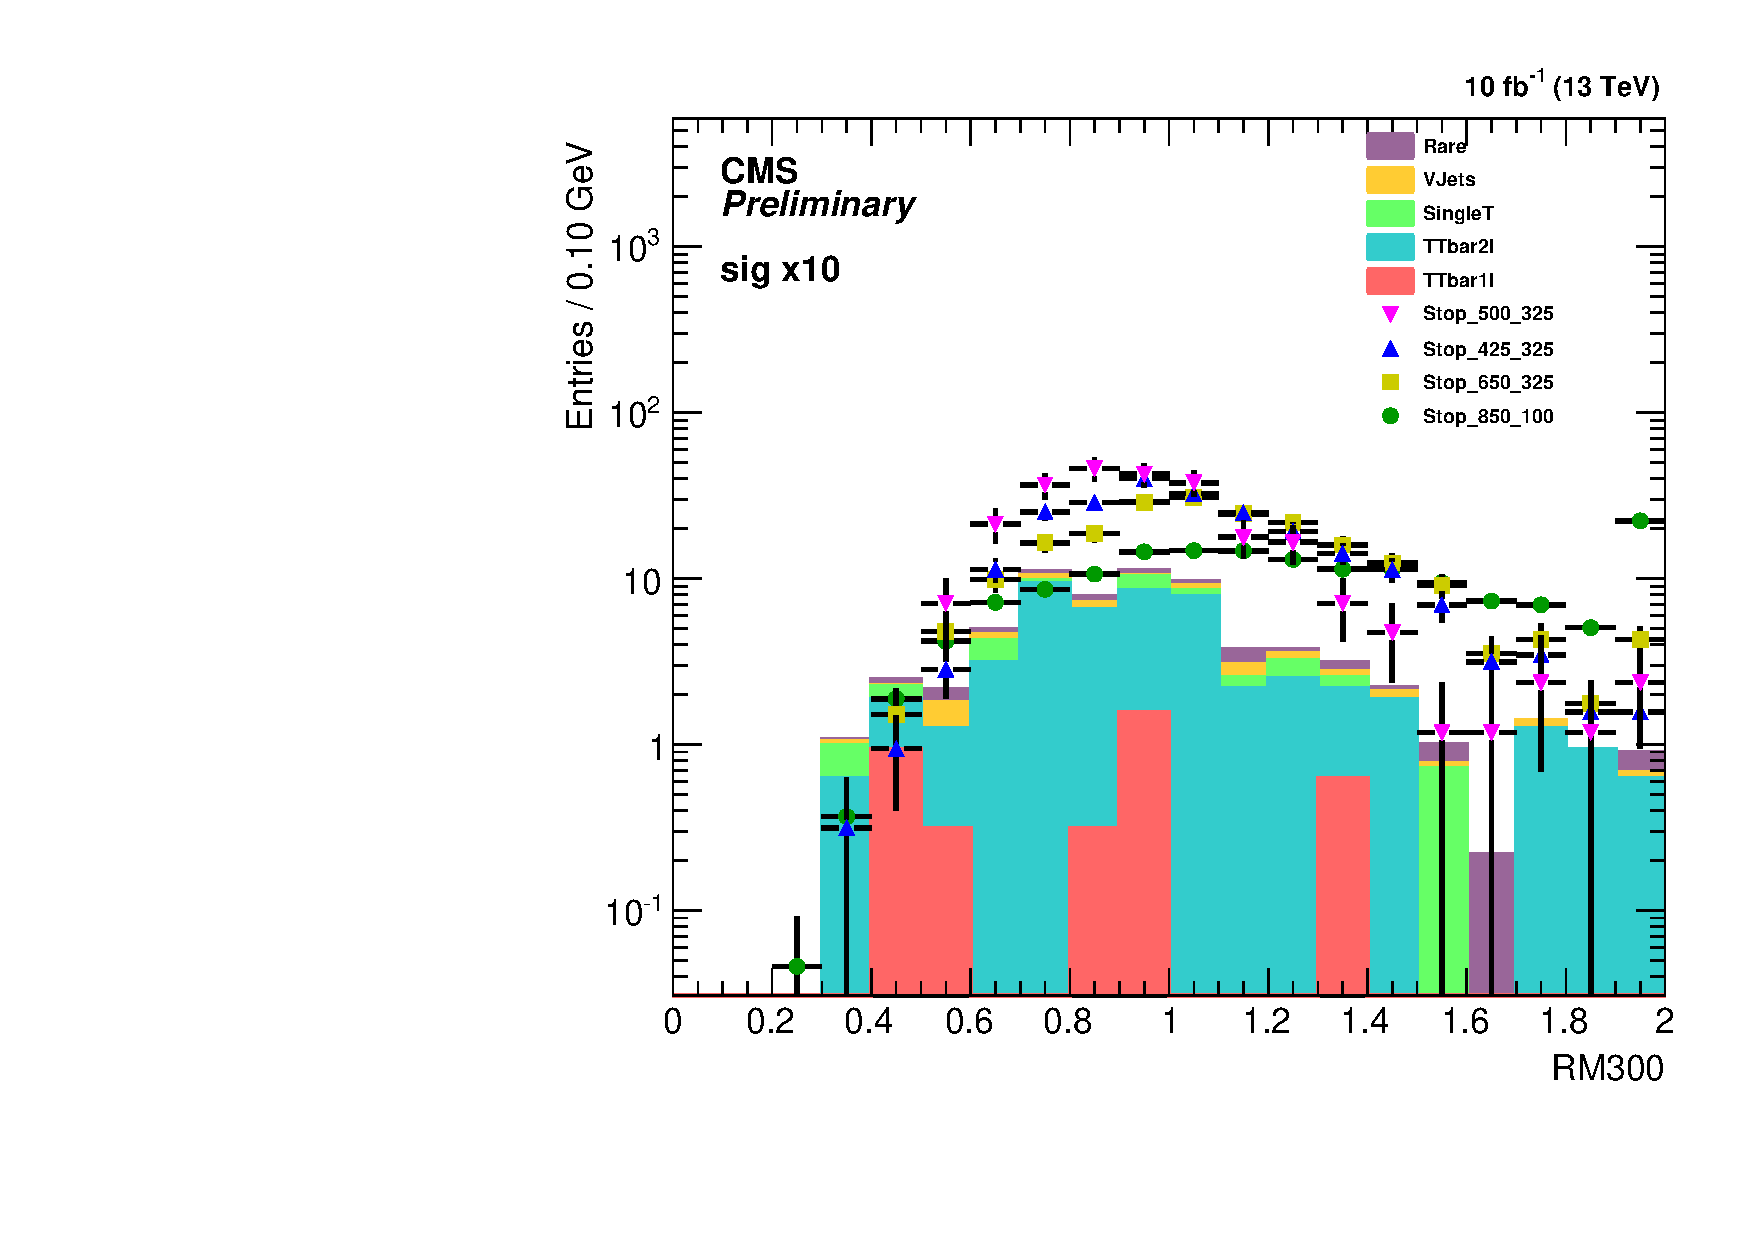
\includegraphics[width=0.49\textwidth]{Figures/SignalVariableStudies/RM300.pdf}
\label{fig:sigvarstudy:RMMTq:RM}
}
\subfigure[$\MT(j_1,\MET)$ distribution.]{
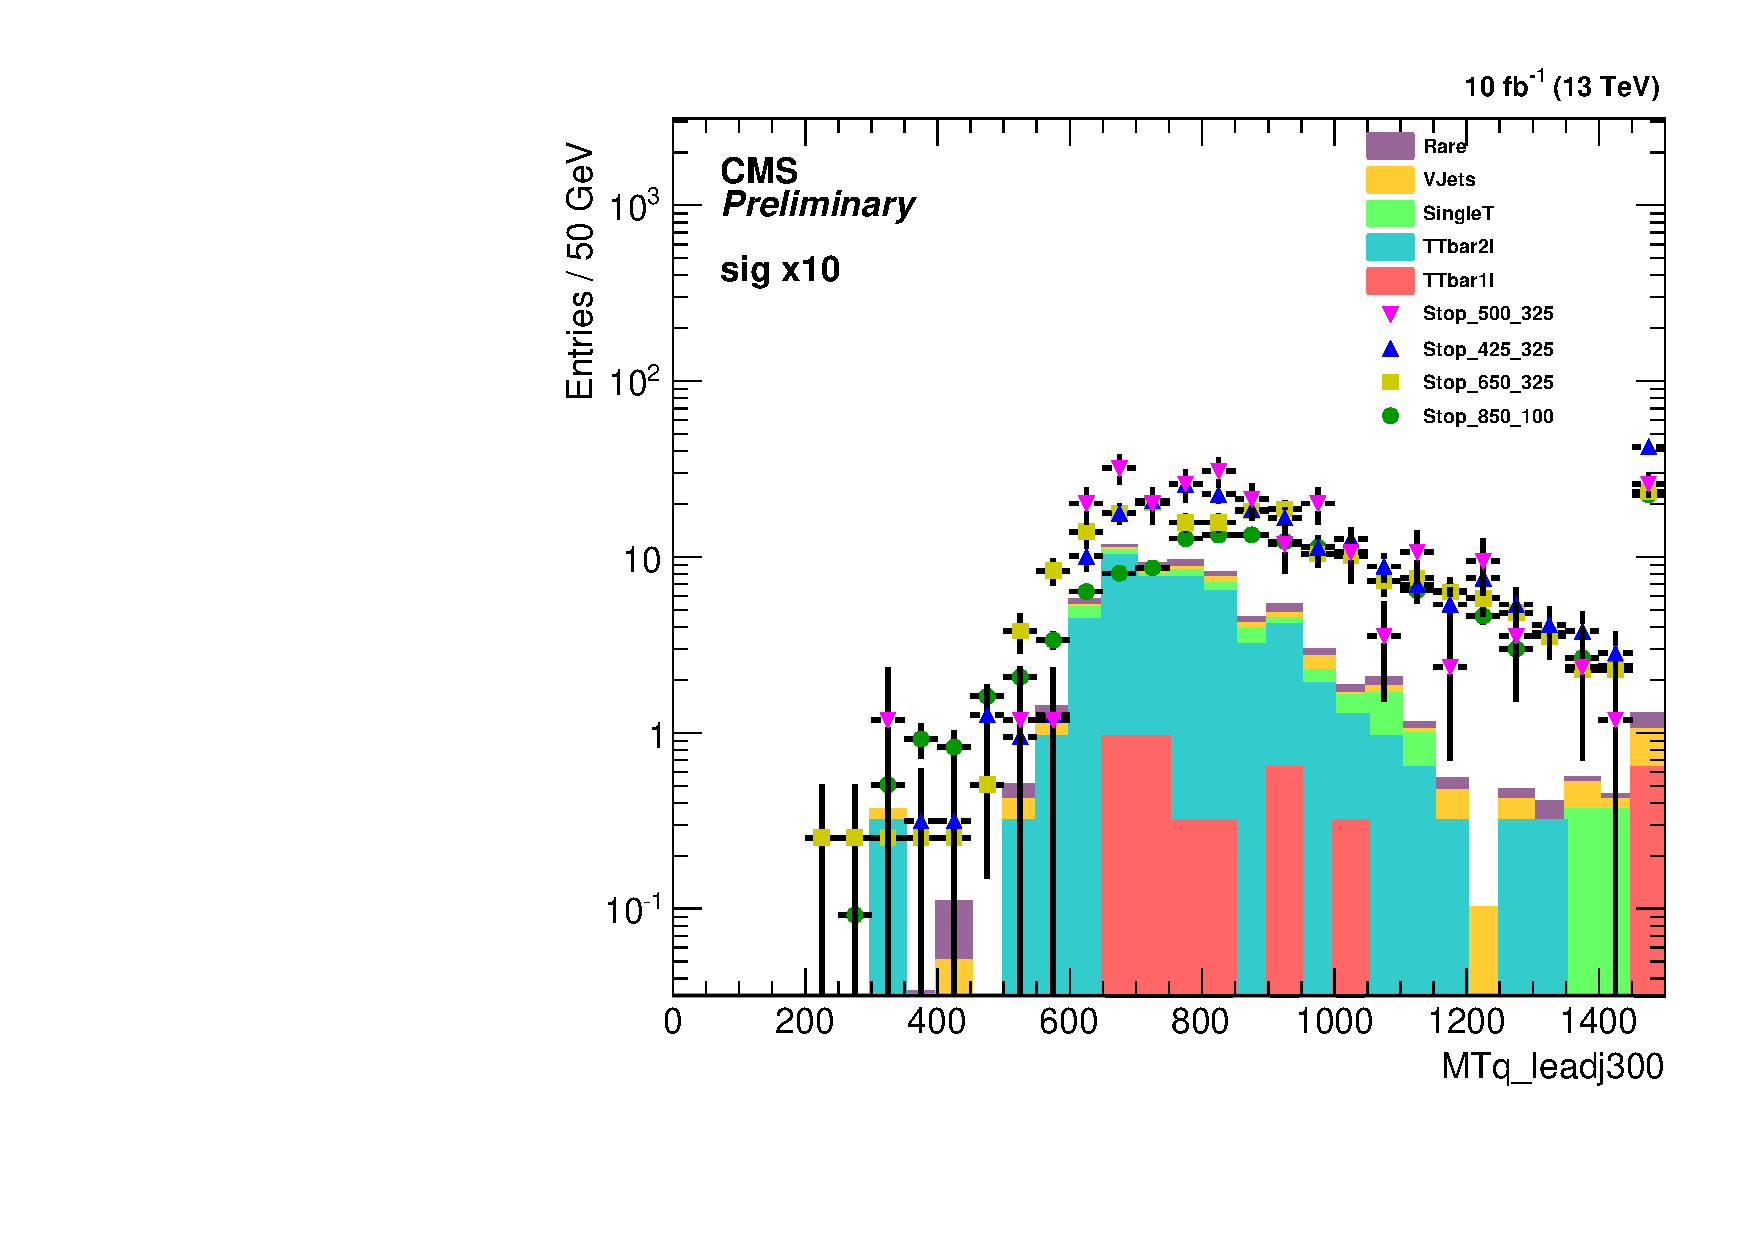
\includegraphics[width=0.49\textwidth]{Figures/SignalVariableStudies/MTq_leadj300.pdf}
\label{fig:sigvarstudy:RMMTq:MTq}
}
\caption{\label{fig:sigvarstudy:RMMTq} $R_M$ (left) and $\MT(j_1,\MET)$ (right) distributions.}
\end{figure}

\subsubsection{$\MT(j_1,\MET)$}

Similar to the motivation of $R_M$, the $\MT(j_1,\MET)$  variable targets the compressed spectra. Instead of a transverse momentum ratio, the transverse mass is computed:
\begin{equation}
\MT(j_1,\MET) = \sqrt{2\MET\pt^{j_1}(1-\cos\phi)},
\end{equation}
where $\phi$ is the angle between the \ptvec of the leading jet and \VEtmiss.
For the leading jet, we require $\pt>300\GeV$.

Figure~\ref{fig:sigvarstudy:RMMTq:MTq} shows the $\MT(j_1,\MET)$ distribution after preselection plus $\MET>300\GeV$. As a test selection $\MT(j_1,\MET)>750\GeV$ was chosen.

\subsection{Signal variable sensitivity for \texorpdfstring{$10\fbinv$}{10 fbinv}}
\label{sec:sigvarstudy:sensitivity}

As mentioned above, this study was performed under a slightly different preselection (especially regarding the second lepton veto) and under the assumption of a luminosity of 10\fbinv.
Therefore, the numbers quoted in this section should not be compared with any result of the main body. They rather serve as a relative comparison for the signal variables under study.

Several figures of merits were studied in this sensitivity study, among them simple S/B and S/$\sqrt{\mathrm{B}}$ checks, with S (B) being signal (background) yield of the signal region selected.
The one quoted here is the $Z_\mathrm{bi}$ variable~\cite{Cousins:2008zz}. We assume a relative background uncertainty of 30\% for this study.

As the preselection was found note to result a good sensitivity for any variable, we don't report its results here. For each variable, we quote numbers for the three other selections in table~\ref{tab:sigvarstudy:sensitivity}. The selection criteria on the variable under study was given in the respective subsections of section~\ref{sec:sigvarstudy:variables}.
%Quote Z_bi here, add the table of Zbis, mention those numbers are for 10/fbinv
\begin{table}[htb]
\begin{center}
\caption{\label{tab:sigvarstudy:sensitivity} Table for $Z_\mathrm{bi}$ values for the four signal mass hypothesis under three different event selections plus a selection on the variable under study. Its criteria is given in the respective subsections of section~\ref{sec:sigvarstudy:variables}.}
\small
\setlength{\tabcolsep}{2pt}
\begin{tabular}{|l|c|c|c|c|c|c|}
\hline
 & \multicolumn{3}{c|}{$M_{\PSQt} = 425\GeV$, $M_{\PSGczDo} = 325\GeV$} & \multicolumn{3}{c|}{$M_{\PSQt} = 500\GeV$, $M_{\PSGczDo} = 325\GeV$} \\
\hline
 Variable & $\MET> 300\GeV$ & $\chi^2_{\mathrm{had.}\cPqt} < 10$ & $\MTtW> 200\GeV$& $\MET> 300\GeV$ & $\chi^2_{\mathrm{had.}\cPqt} < 10$ & $\MTtW> 200\GeV$ \\
 \hline
 $t$ 											& 0.15 & 0.18 & 0.18			& -0.06 & -0.07 & -0.07\\
 $t_\text{mod}$ 									& -0.07 & -0.06 & -0.06		& -0.15 & -0.17 & -0.17\\
 $\MTtW$ 										& 0.16 & 0.20 & 0.20			& -0.03 & -0.02 & -0.02\\
 $\MTt(\ell\cPqb,\cPqb)$ 							& 0.12 & 0.16 & 0.16			& -0.02 & 0.02 & -0.04\\
 $\MTt(\ell\cPqb,\cPqb\cPq\cPq)$  					& 0.02 & 0.09 & 0.14			& -0.05 & -0.02 & -0.05\\
 $\MTt^{M_\mathrm{vis}=0}(\ell\cPqb,\cPqb)$ 			& -0.06 & -0.06 & -0.06		& -0.13 & -0.13 & -0.14\\
 $\MTt^{M_\mathrm{vis}=0}(\ell\cPqb,\cPqb\cPq\cPq)$	& -0.11 & -0.10 & -0.09		& -0.18 & -0.19 & -0.22\\
 $\MT(j_1,\MET)$ 								& 0.31 & 0.40 & 0.33			& 0.30 & 0.41 & 0.06\\
 $R_M$ 										& 0.27 & 0.35 & 0.34			& 0.26 & 0.34 & 0.13\\
 $\MTt(\ell,\cPq\cPq)$ 							& 0.01 & 0.06 & 0.04			& -0.07 & -0.03 & -0.12\\
 $\MTt^{M_\mathrm{vis}=0}(\ell,\cPq\cPq)$  			& -0.04 & -0.02 & -0.04		& -0.13 & -0.11 & -0.16\\
 \hline\hline
  & \multicolumn{3}{c|}{$M_{\PSQt} = 650\GeV$, $M_{\PSGczDo} = 325\GeV$} & \multicolumn{3}{c|}{$M_{\PSQt} = 850\GeV$, $M_{\PSGczDo} = 100\GeV$} \\
  \hline
 Variable & $\MET> 300\GeV$ & $\chi^2_{\mathrm{had.}\cPqt} < 10$ & $\MTtW> 200\GeV$& $\MET> 300\GeV$ & $\chi^2_{\mathrm{had.}\cPqt} < 10$ & $\MTtW> 200\GeV$ \\
 \hline
  $t$ 											& 0.66 & 0.78 & 0.78			& 0.48 & 0.57 & 0.57\\
  $t_\text{mod}$ 								& 0.90 & 1.04 & 1.01			& 0.68 & 0.79 & 0.78\\
  $\MTtW$ 									& 0.69 & 0.84 & 0.84			& 0.42 & 0.53 & 0.53\\
  $\MTt(\ell\cPqb,\cPqb)$ 							& 0.42 & 0.57 & 0.63			& 0.27 & 0.38 & 0.47\\
  $\MTt(\ell\cPqb,\cPqb\cPq\cPq)$  					& 0.20 & 0.32 & 0.51			& 0.16 & 0.32 & 0.58\\
  $\MTt^{M_\mathrm{vis}=0}(\ell\cPqb,\cPqb)$ 			& 0.55 & 0.66 & 0.76			& 0.40 & 0.47 & 0.61\\
  $\MTt^{M_\mathrm{vis}=0}(\ell\cPqb,\cPqb\cPq\cPq)$	& 0.55 & 0.70 & 0.89			& 0.38 & 0.51 & 0.76\\
  $\MT(j_1,\MET)$ 								& 0.22 & 0.31 & 0.42			& 0.16 & 0.23 & 0.48\\
  $R_M$ 										& 0.24 & 0.33 & 0.52			& 0.14 & 0.20 & 0.51\\
  $\MTt(\ell,\cPq\cPq)$ 							& 0.44 & 0.62 & 0.90			& 0.21 & 0.33 & 0.69\\
  $\MTt^{M_\mathrm{vis}=0}(\ell,\cPq\cPq)$  			& 0.45 & 0.62 & 0.91			& 0.22 & 0.33 & 0.68\\
 \hline
\end{tabular}
\end{center}
\end{table}

From this table we find the following: 

For the two mass points of larger mass splitting between the top squark and LSP masses, the most sensitive variable is the modified topness variable. Also good sensitivity is reached for the massless $\MTt(\ell\cPqb,\cPqb\cPq\cPq)$ variable, and the $\MTt(\ell,\cPq\cPq)$ variables. 
For the most sensitive variable we find the best separation without the \MTtW selection. 

For the two mass points with smaller mass splitting between the top squark and LSP masses, the most sensitive variables are the $R_M$ and $\MT(j_1,\MET)$ variables. The \MTtW and  $\MTt(\ell\cPqb,\cPqb)$, $\MTt(\ell\cPqb,\cPqb\cPq\cPq)$ variables also have some sensitivity, although the highest sensitivity is achieved before putting a selection on \MTtW.\\

This results need to be handled with care out of three reasons:
\begin{itemize}
\item Systematic/statistical uncertainties: In principle, the uncertainty value chosen can change the relative sensitivity. However, a relative background uncertainty of 10\% or 50\% the results are confirmed.
\item Total data yield: This numbers were obtained for 10\fbinv. For 2015 data we expect a data sample of 2-3\fbinv. These can change the conclusion significantly, as shown for one example below, when comparing topness versus \MTtW.
\item Simplified event selection: This study was performed with a single \MET selection of $\MET>300\GeV$. The final analysis has a \MET-binning approach with multiple signal regions along the \MET distribution. Depending on the correlation of the investigated variables and the \MET variable, this might lead to changes in the results. Also the $\chi^2_{\mathrm{had.}\cPqt}$ variable was calculated with a simplied jet energy resolution of 10\%.
\end{itemize}

One example, where these results did not agree with the strategy for 2015 data is shown in section~\ref{sec:sigvarstudy:MT2WvsTopness}.

\subsection{\texorpdfstring{\MTtW}{MT2W} versus (modified) topness}
\label{sec:sigvarstudy:MT2WvsTopness}

In figure~\ref{fig:sigvarstudy:MT2WvsTopness:ROC}, the ROC curves (signal efficiency versus background efficiency) for the two high mass points for the three variables \MTtW, and (modified) topness are compared.
\begin{figure}
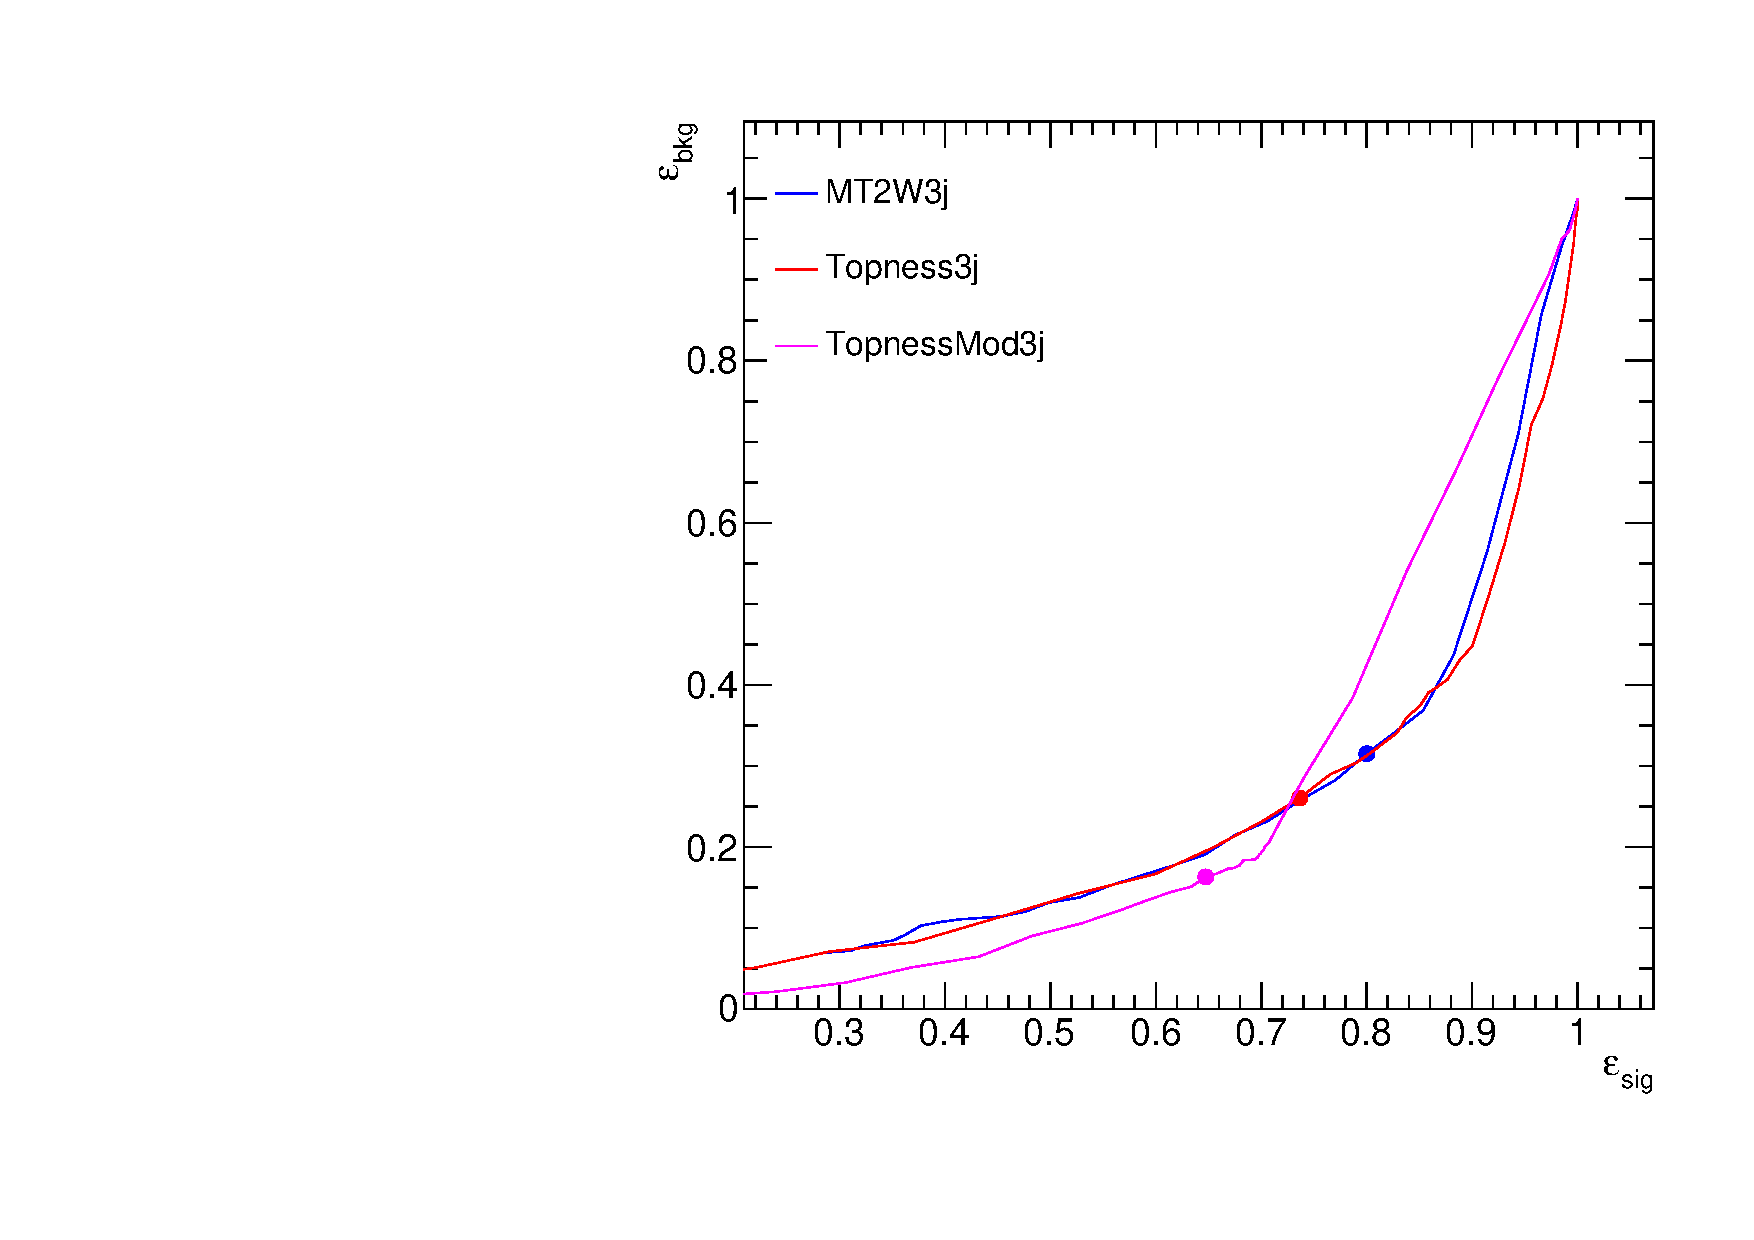
\includegraphics[width=0.49\textwidth]{Figures/SignalVariableStudies/ROC_j3Compare_Stop_850_100.pdf}
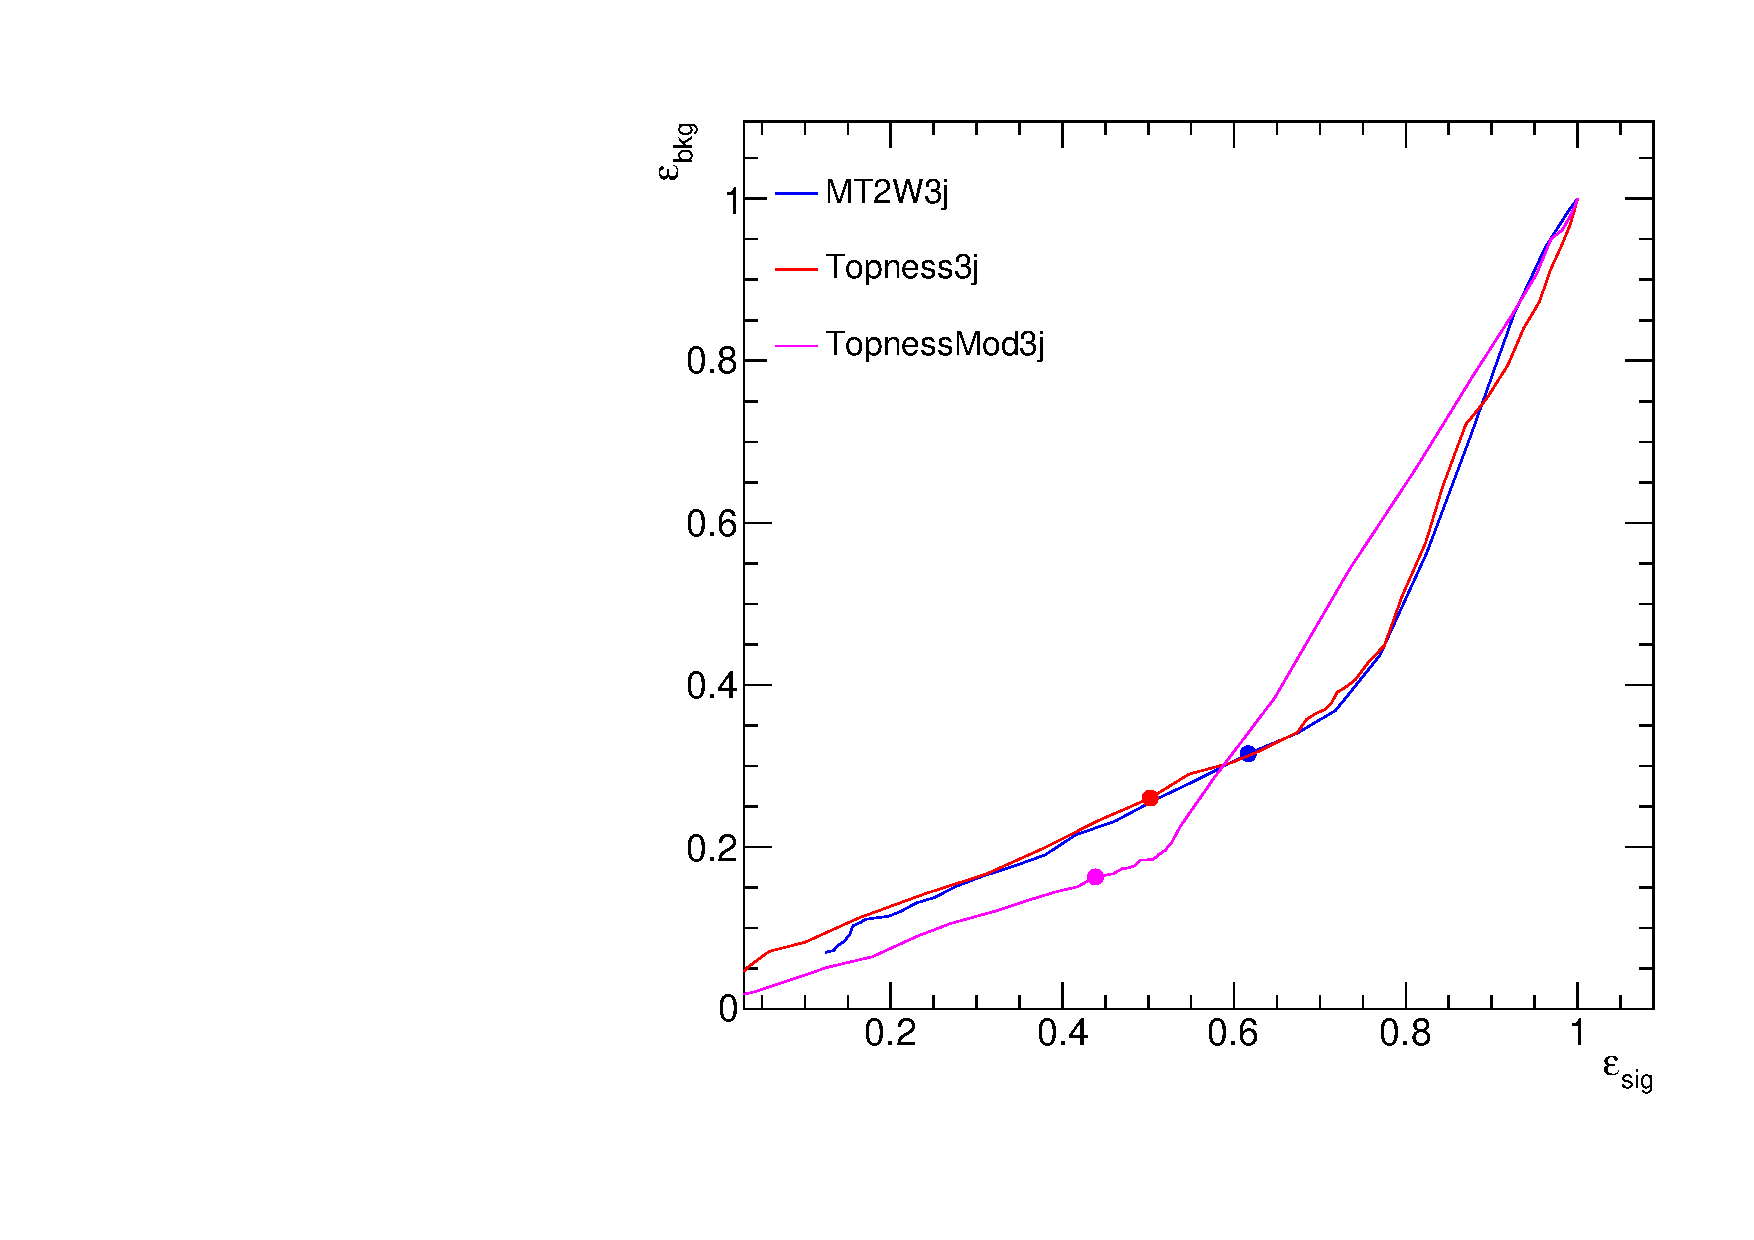
\includegraphics[width=0.49\textwidth]{Figures/SignalVariableStudies/ROC_j3Compare_Stop_650_325.pdf}
\caption{\label{fig:sigvarstudy:MT2WvsTopness:ROC} ROC curves for the floating \MTtW, and (modified) topness selection criteria for $M_{\PSQt} = 850\GeV$, $M_{\PSGczDo} = 100\GeV$ (left) and $M_{\PSQt} = 650\GeV$, $M_{\PSGczDo} = 325\GeV$ (right). The dots correspond to $\MTtW>200\GeV$ , $t> 9$, and $t_\mathrm{mod}> 7$.}
\end{figure}

The overall signal efficiency for the \MTtW selection is about 1/3 higher with respect to the modified topness selection.
We found, that already 5\fbinv, the significance ($Z_\mathrm{bi}$ value) reach an similar value, for less data, the \MTtW selection reaches higher values. Therefore, for the first round of this search with 2015 data, we chose to use the \MTtW variable as one signal variable.

When we accumulate more data, we will reevaluate this: We might either switch to the modified topness variable or choose to set harder selections on \MET.

A similar argument was found for the $R_M$ and $\MT(j_1,\MET)$  variables. The \MET selection already reduces the overall signal yield to small values for the lighter mass point signals. Thus, an additional selection on those variable decrease the signal yield, and do not result in a gain the overall signal sensitivity for the amount of data that will be selected in 2015.

\subsection{\texorpdfstring{\MET}{MET} versus \texorpdfstring{$\MET\sqrt{\HT}$}{MET/sqrt(HT)}}

Similar to the study in section~\ref{sec:sigvarstudy:MT2WvsTopness}, variants of the \MET variable were compared. One promising variable was $\MET\sqrt{\HT}$, where \HT is the scalar jet-\pt sum. Also a variant with \HT plus lepton-\pt was investigated. As figure~\ref{fig:sigvarstudy:METvsMETsqrtHT:ROC} shows, the plain \MET variable performs strongest.
\begin{figure}
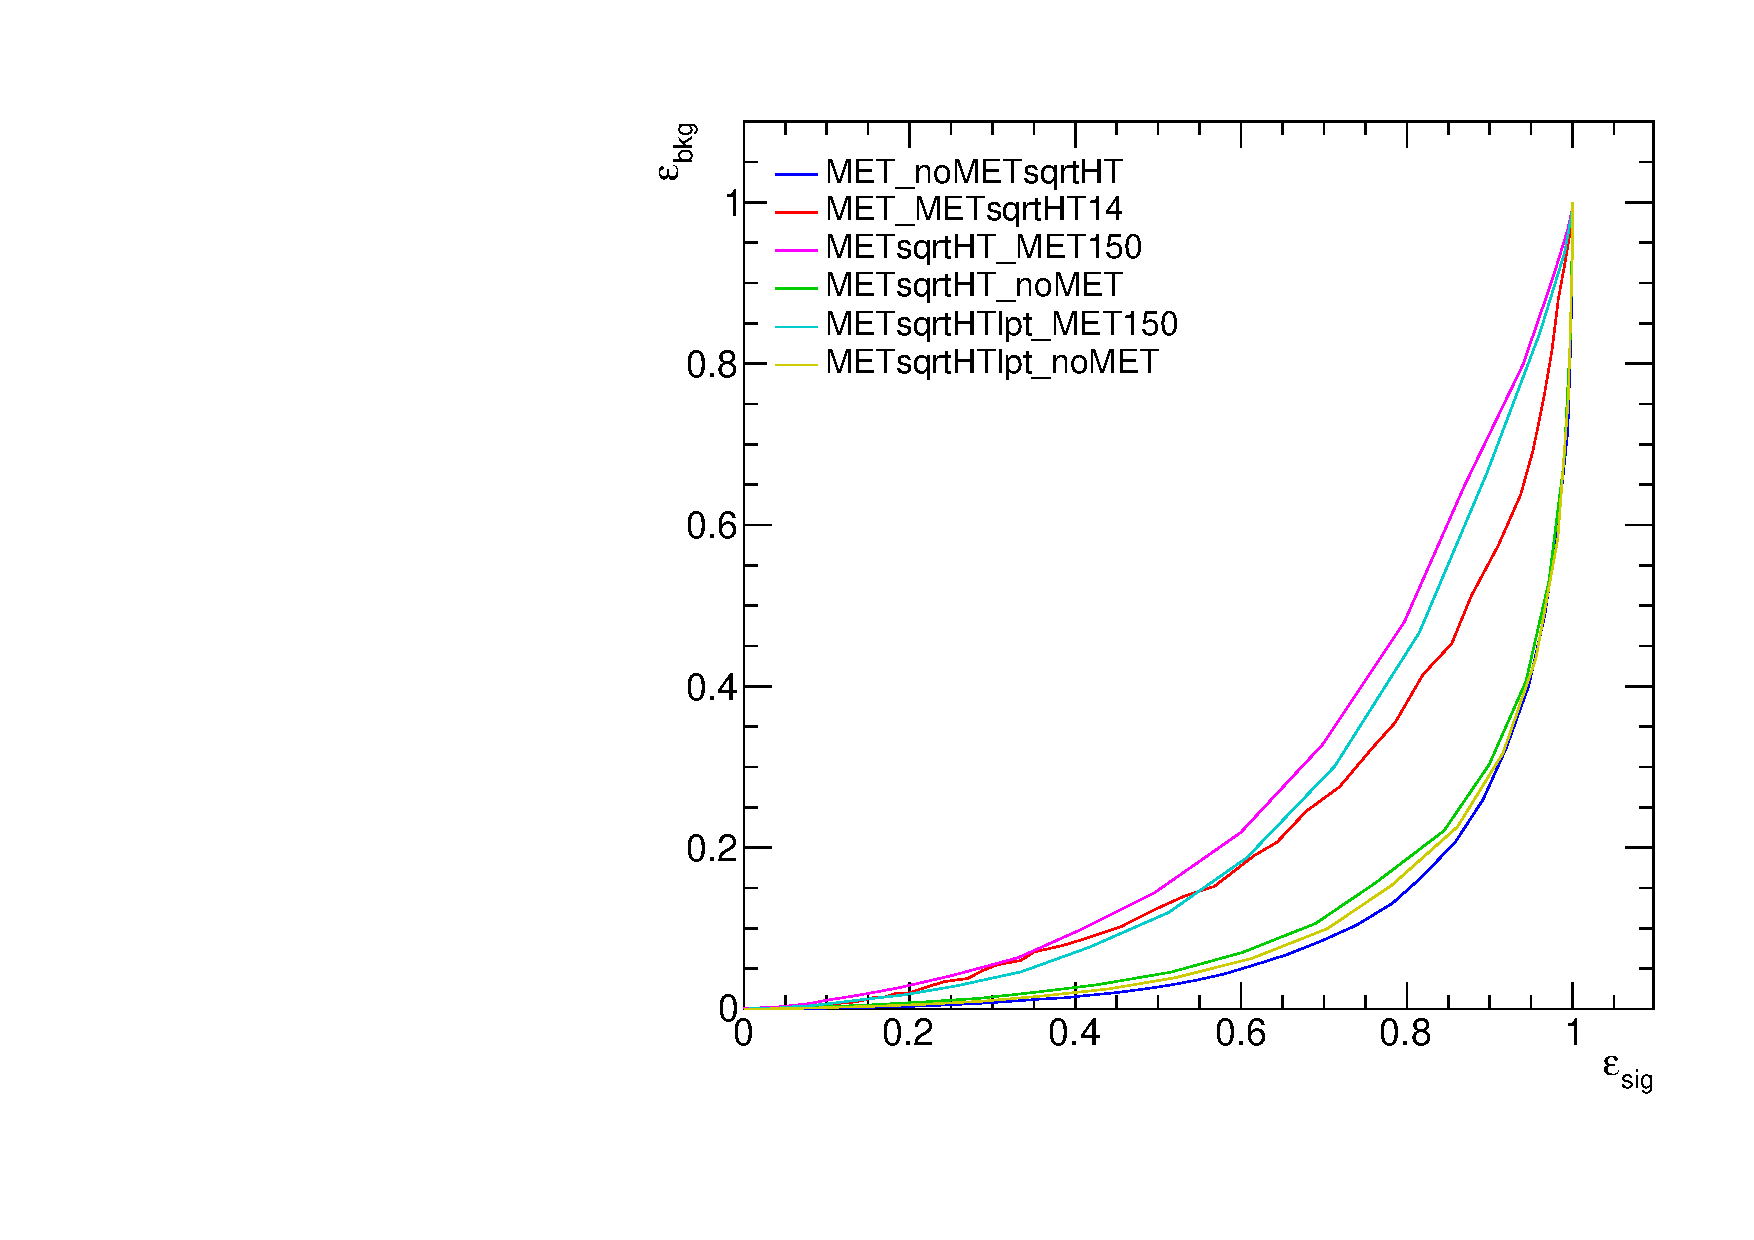
\includegraphics[width=0.49\textwidth]{Figures/SignalVariableStudies/ROC_METCompare_Stop_425_325.pdf}
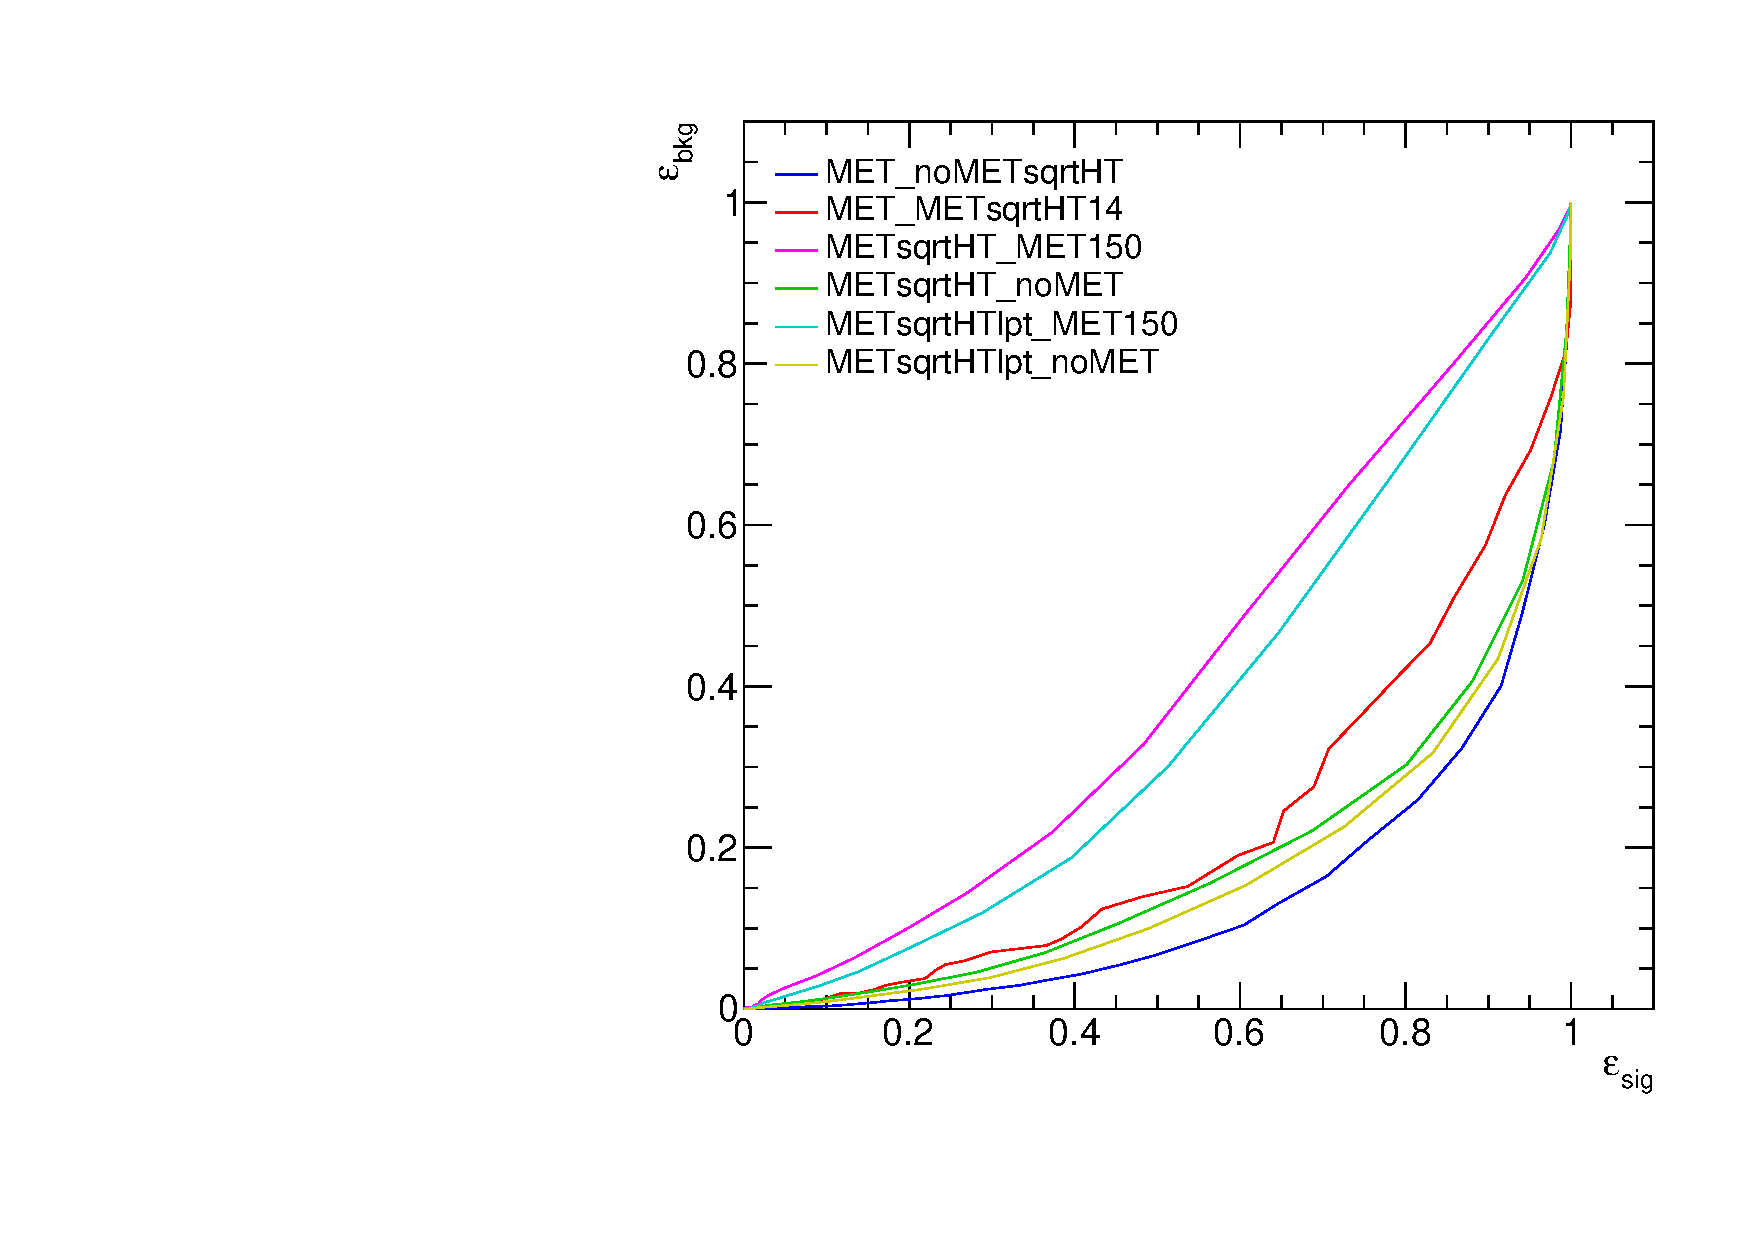
\includegraphics[width=0.49\textwidth]{Figures/SignalVariableStudies/ROC_METCompare_Stop_500_325.pdf}
\caption{\label{fig:sigvarstudy:METvsMETsqrtHT:ROC} ROC curves for the floating \MET, $\MET\sqrt{\HT}$ and $\MET\sqrt{\HT+\ell\text{-}\pt}$ criteria for $M_{\PSQt} = 425\GeV$, $M_{\PSGczDo} = 325\GeV$ (left) and $M_{\PSQt} = 500\GeV$, $M_{\PSGczDo} = 325\GeV$ (right). The various curves are more separated for the two higher signal mass points.}
\end{figure}

The studies of this appendix led to the signal region definitions of \MET and \MTtW as described in section~\ref{sec:obj_sel:signal_regions}.

\subsection{Discussion}

Even for 5\fbinv, the topness or modified topness variable don't increase the significance with respect of the usage of the \MTtW variable. The \MTt variable results in a greater background rejection for a working point with high signal efficiency. The modified topness variable, on the other hand, has a superior background rejection when choosing a working point with low signal efficiency.
Therefore, for an analysis of a large data sample ($>10\fbinv$), one might consider changing the selection of \MTtW to modified topness. However, as other variables will also play a role, a definite answer cannot be given at this stage of the analysis.

For compressed signals, we saw that both $R_M$ and $\MT(j_1,\MET)$ can improve the signal efficiency. As it was shown above {\color{red} ADD REFERENCE TO DANS STUDY}, for the current data sample, a simple selection on the leading jet-\pt is the most efficient selection one can do. The additional information in $R_M$ or $\MT(j_1,\MET)$ does not bring a large gain so far.





\section{Signal variable studies for T2tb and T2bW like signatures}
\label{sec:sigvarstudy2}

\emph{Please note: that this study has been performed under the assumption of 3\fbinv. Final studies (SEE DISCUSSION) led to the conclusion that for a datasample of 2\fbinv, there is no possibility to increase the significance including new signal variables, as such an additional binning leads to signal regions which have $\lesssim2$ signal events even with $\MET>250\GeV$.}

\emph{However, we include the discussion here for future reference.}

This appendix discusses investigations on various variables suitable for signal discriminating variables. As signal we have several mass points of top squark pair production where both top squark decays are $\PSQt\to\cPqb\PSGcpmDo$, $\PSGcpmDo\to\PW\PSGczDo$ (``T2bW''). We also obtimized this including signals where we have a mixture of the decay mentioned above and decays like $\PSQt\to\cPqt\PSGczDo$ (``T2tb'').
For defining event selections, we considered signal region selection sensitive to all three modes (T2tt, T2tb, and T2bW).

Therefore, the above discussion of section~\ref{sec:sigvarstudy} is valid here, and won't be repeated.

The event selection for this study is the same as the one quoted in section~\ref{sec:sigvarstudy:evtselection}, with the exception that we use the proper second lepton veto (including isolated track and tau vetos) of the analysis, see section~\ref{sec:obj_sel:lepton_sel}.

\subsection{Signal variables under study}
\label{sec:sigvarstudy:variables2}

\subsubsection{$M_{\ell\cPqb}$}

The invariant of the lepton--b-jet pair coming from the same top quark decay should, for perfect resolution, have an endpoint at $M_{\ell\cPqb} \approx 153\GeV$. For a T2bW-like signature, this bound does not exist. In fact the bound for a T2bW-like signature will be at 
\begin{equation*}
M_{\ell\cPqb} = M(\PSQt_1) \left(1-\frac{M^2(\PSGcpmDo)}{M^2(\PSQt_1)}\right)
\end{equation*}

Therefore, this variable could greatly reduce the background for dileptonic $\cPqt\cPaqt+$jets.

Figure~\ref{fig:sigvarstudy:MlbDRlb:Mlb} shows the $M_{\ell \cPqb}$ distribution with the b-jet chosen to be the jet with the highest CSV discriminant. Other selections of the b-jet show virtually the same discrimination.

As it can be appreciated, for a T2bW-like signatures, most of the background is below $M_{\ell\cPqb} < 175\GeV$, thus this variable can potentially greatly increase the sensitivity for this signal.
As the T2tt-like signatures have a very similar distribution as the $\cPqt\cPaqt+$jets background, we always want to keep a selection, that also includes events with the low $M_{\ell\cPqb}$.

\begin{figure}
\subfigure[$M_{\ell \cPqb}$ distribution.]{
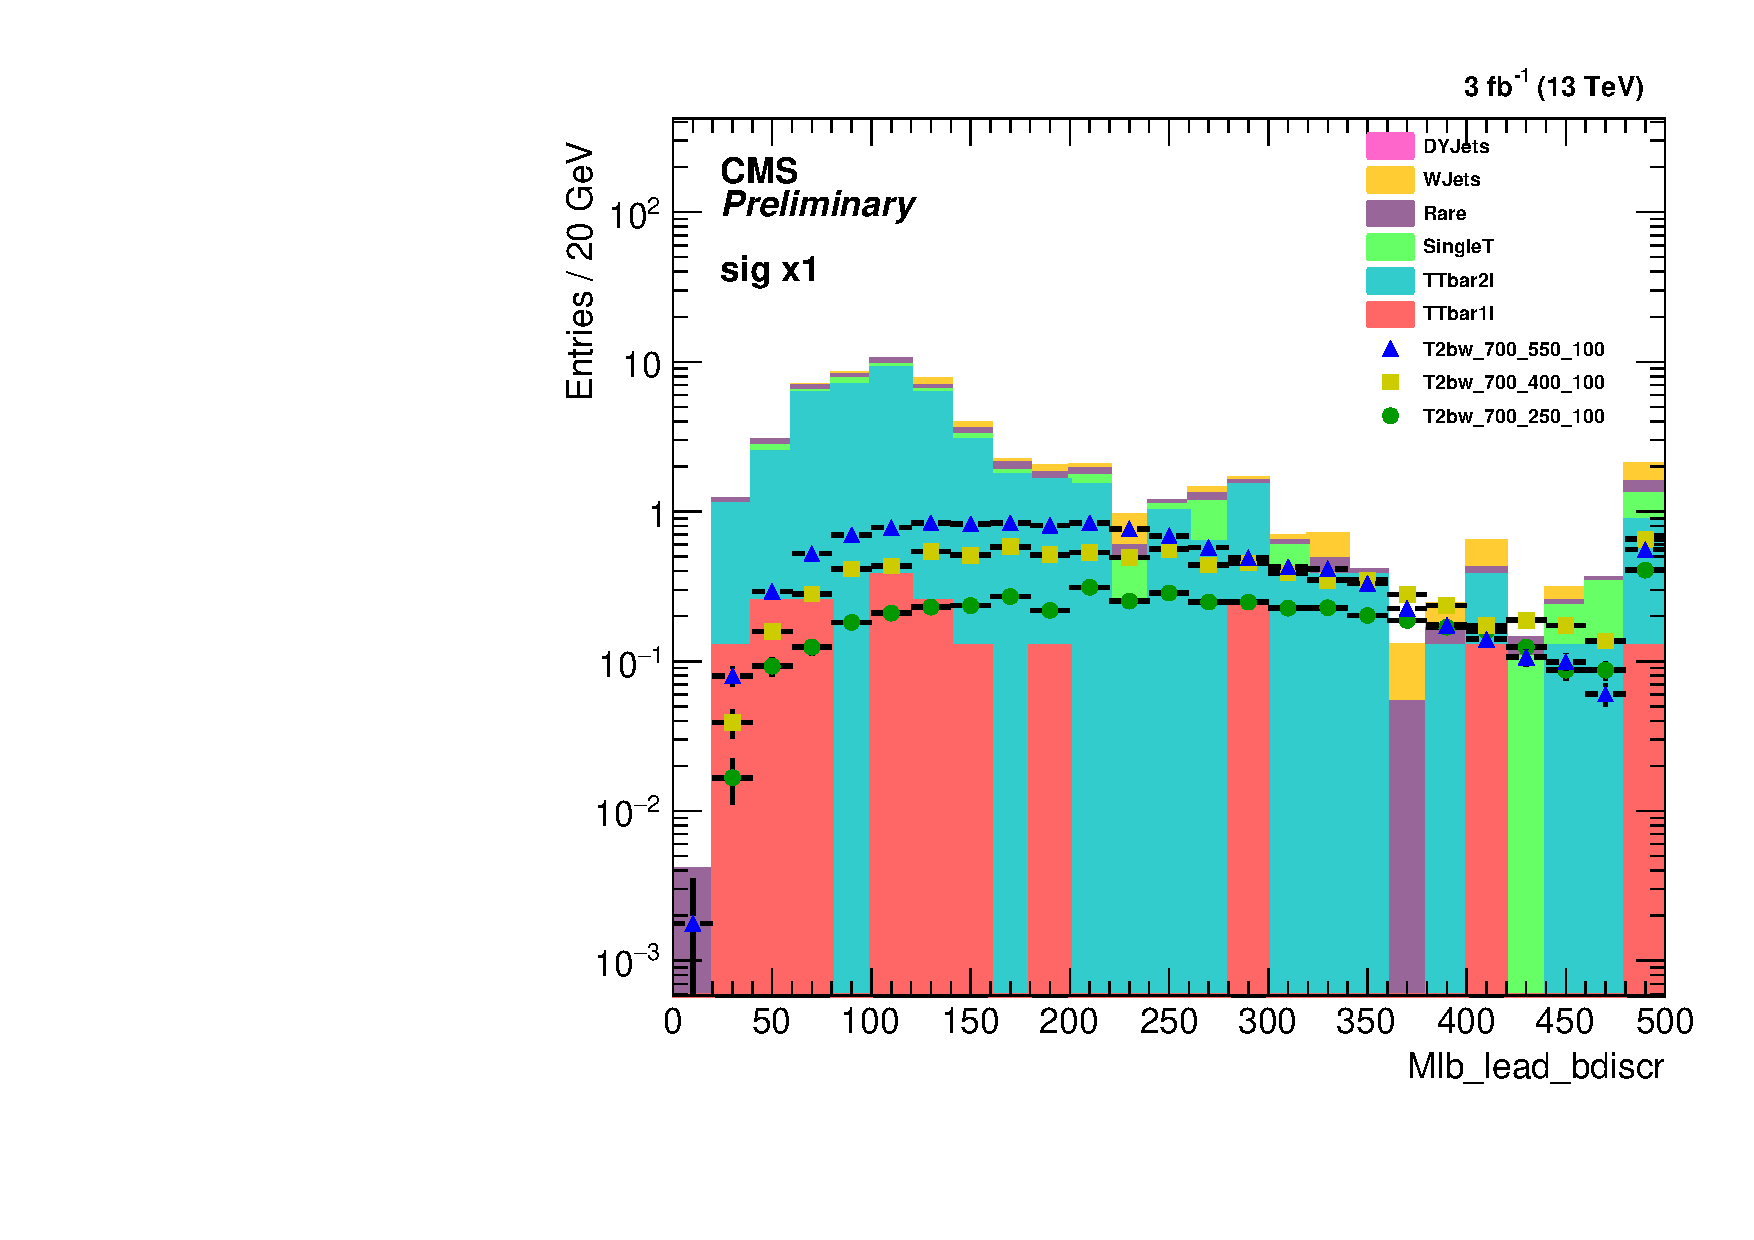
\includegraphics[width=0.49\textwidth]{Figures/SignalVariableStudies/Mlb_lead_bdiscr.pdf}
\label{fig:sigvarstudy:MlbDRlb:Mlb}
}
\subfigure[$\Delta R(\ell \cPqb)$ distribution.]{
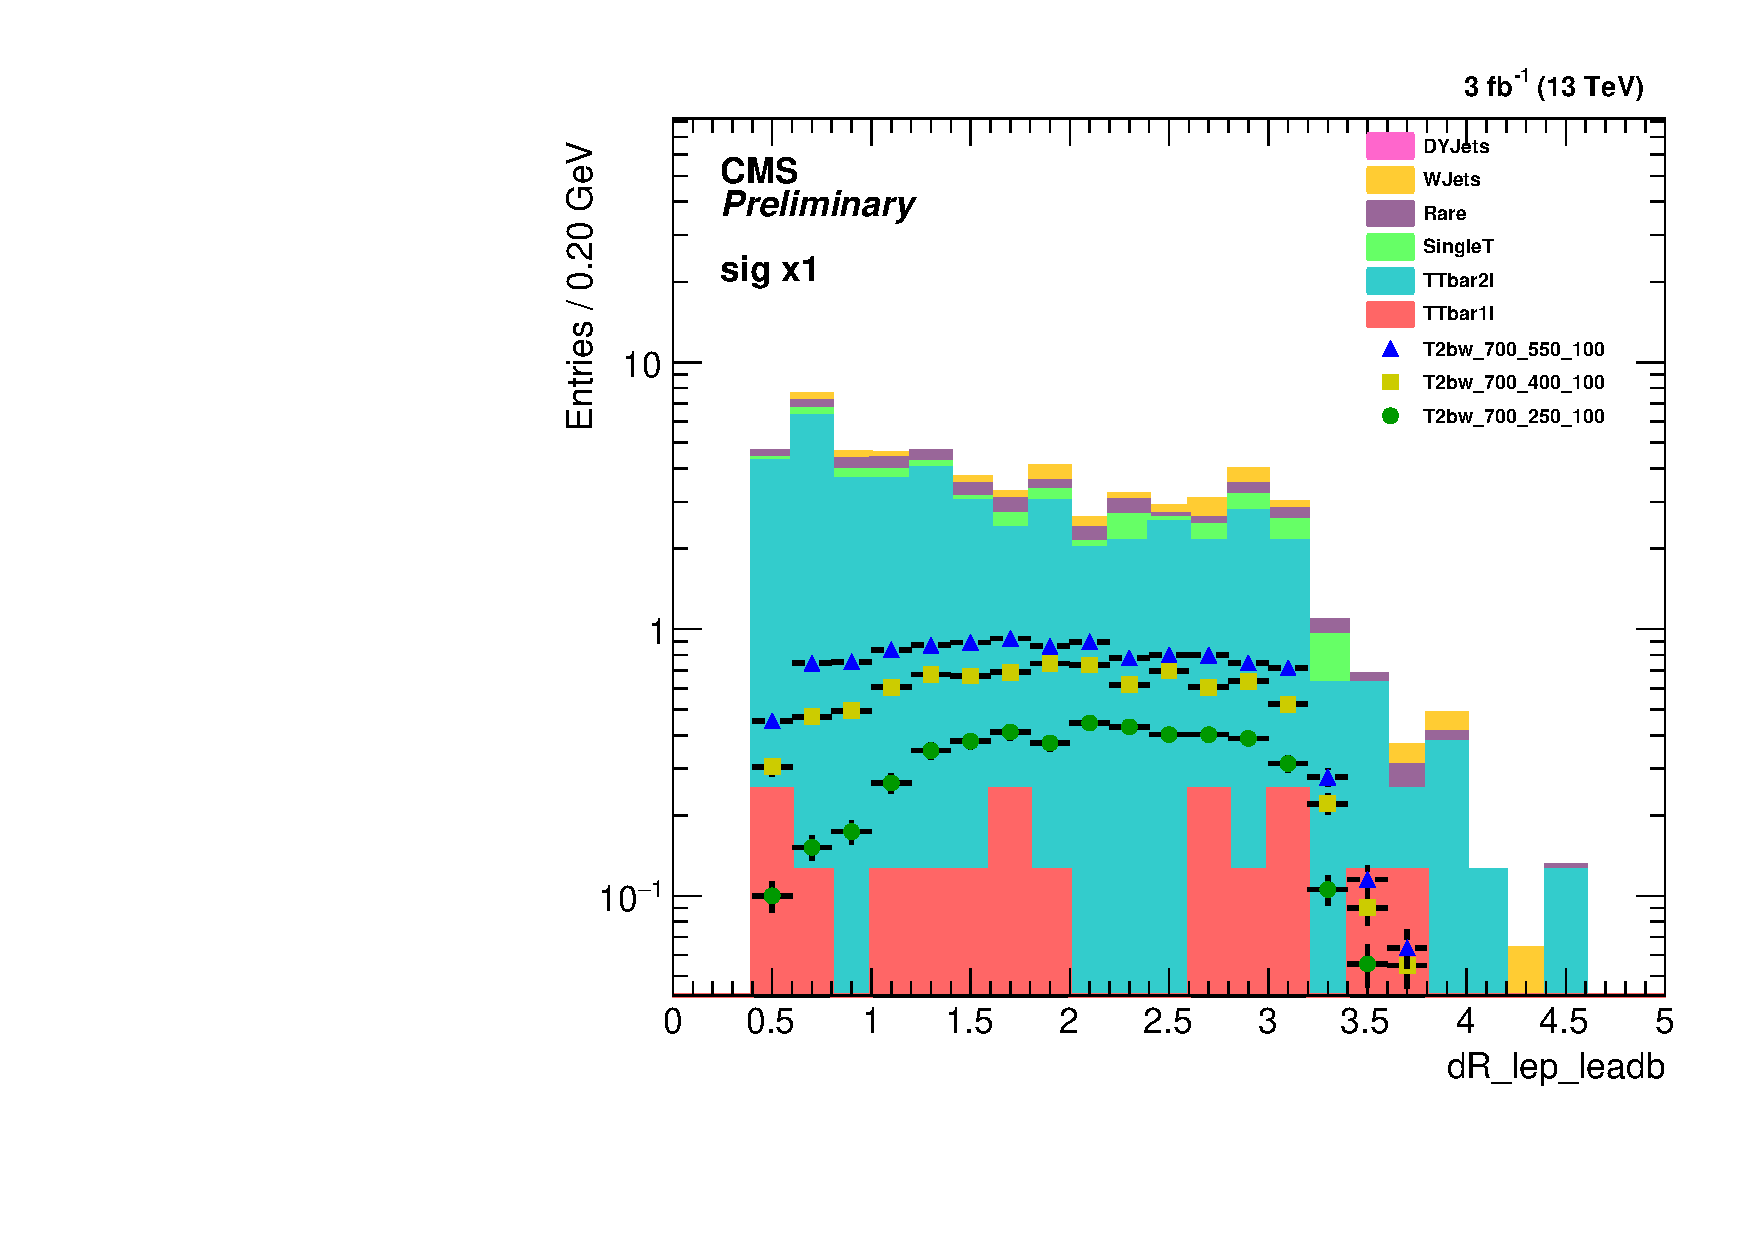
\includegraphics[width=0.49\textwidth]{Figures/SignalVariableStudies/dR_lep_leadb.pdf}
\label{fig:sigvarstudy:MlbDRlb:DRlb}
}
\caption{\label{fig:sigvarstudy:MlbDRlb} $M_{\ell \cPqb}$ (left) and $\Delta R(\ell \cPqb)$ (right) distributions.}
\end{figure}

\subsubsection{$\Delta R(\ell\cPqb)$}

In the 8 TeV analysis~\cite{Chatrchyan:2013xna}, $\Delta R(\ell\cPqb)$ had been used in the event selection.
The distribution of $\Delta R(\ell \cPqb)$ is shown in fig.~\ref{fig:sigvarstudy:MlbDRlb:DRlb}. We clearly see, that the discrimination is weaker. Maybe, this variable could be used in a multivariate analysis.

\subsubsection{Leading b-jet-\pt}

If the mass splitting between the top squark and the chargino is large, the b-jet produced in the top squark decay can be very boosted. In such a case, we expect great discrimination in the distribution of the leading b-jet-\pt. This is confirmed in fig.~\ref{fig:sigvarstudy:bptlpt:bpt}.

\begin{figure}
\subfigure[Leading b-jet-\pt distribution.]{
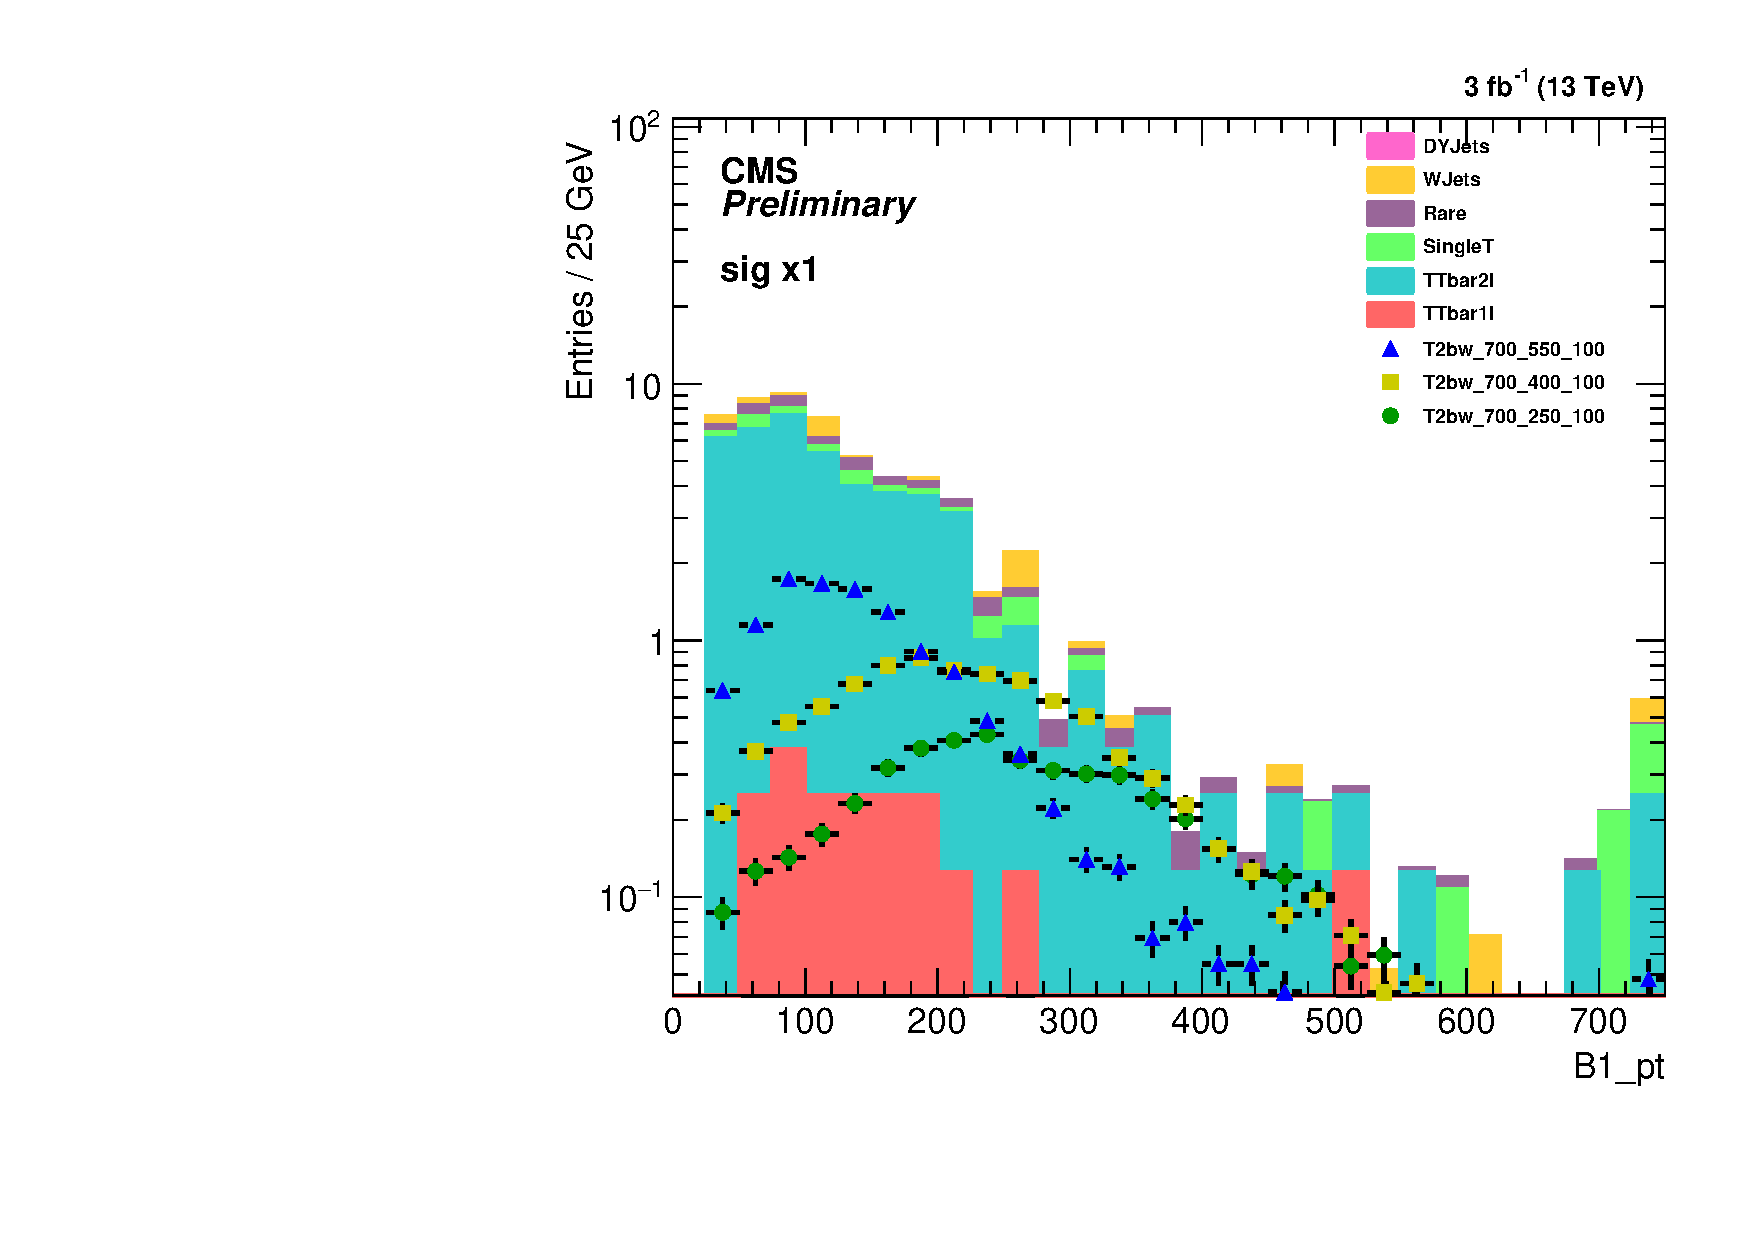
\includegraphics[width=0.49\textwidth]{Figures/SignalVariableStudies/B1_pt.pdf}
\label{fig:sigvarstudy:bptlpt:bpt}
}
\subfigure[:epton-\pt distribution.]{
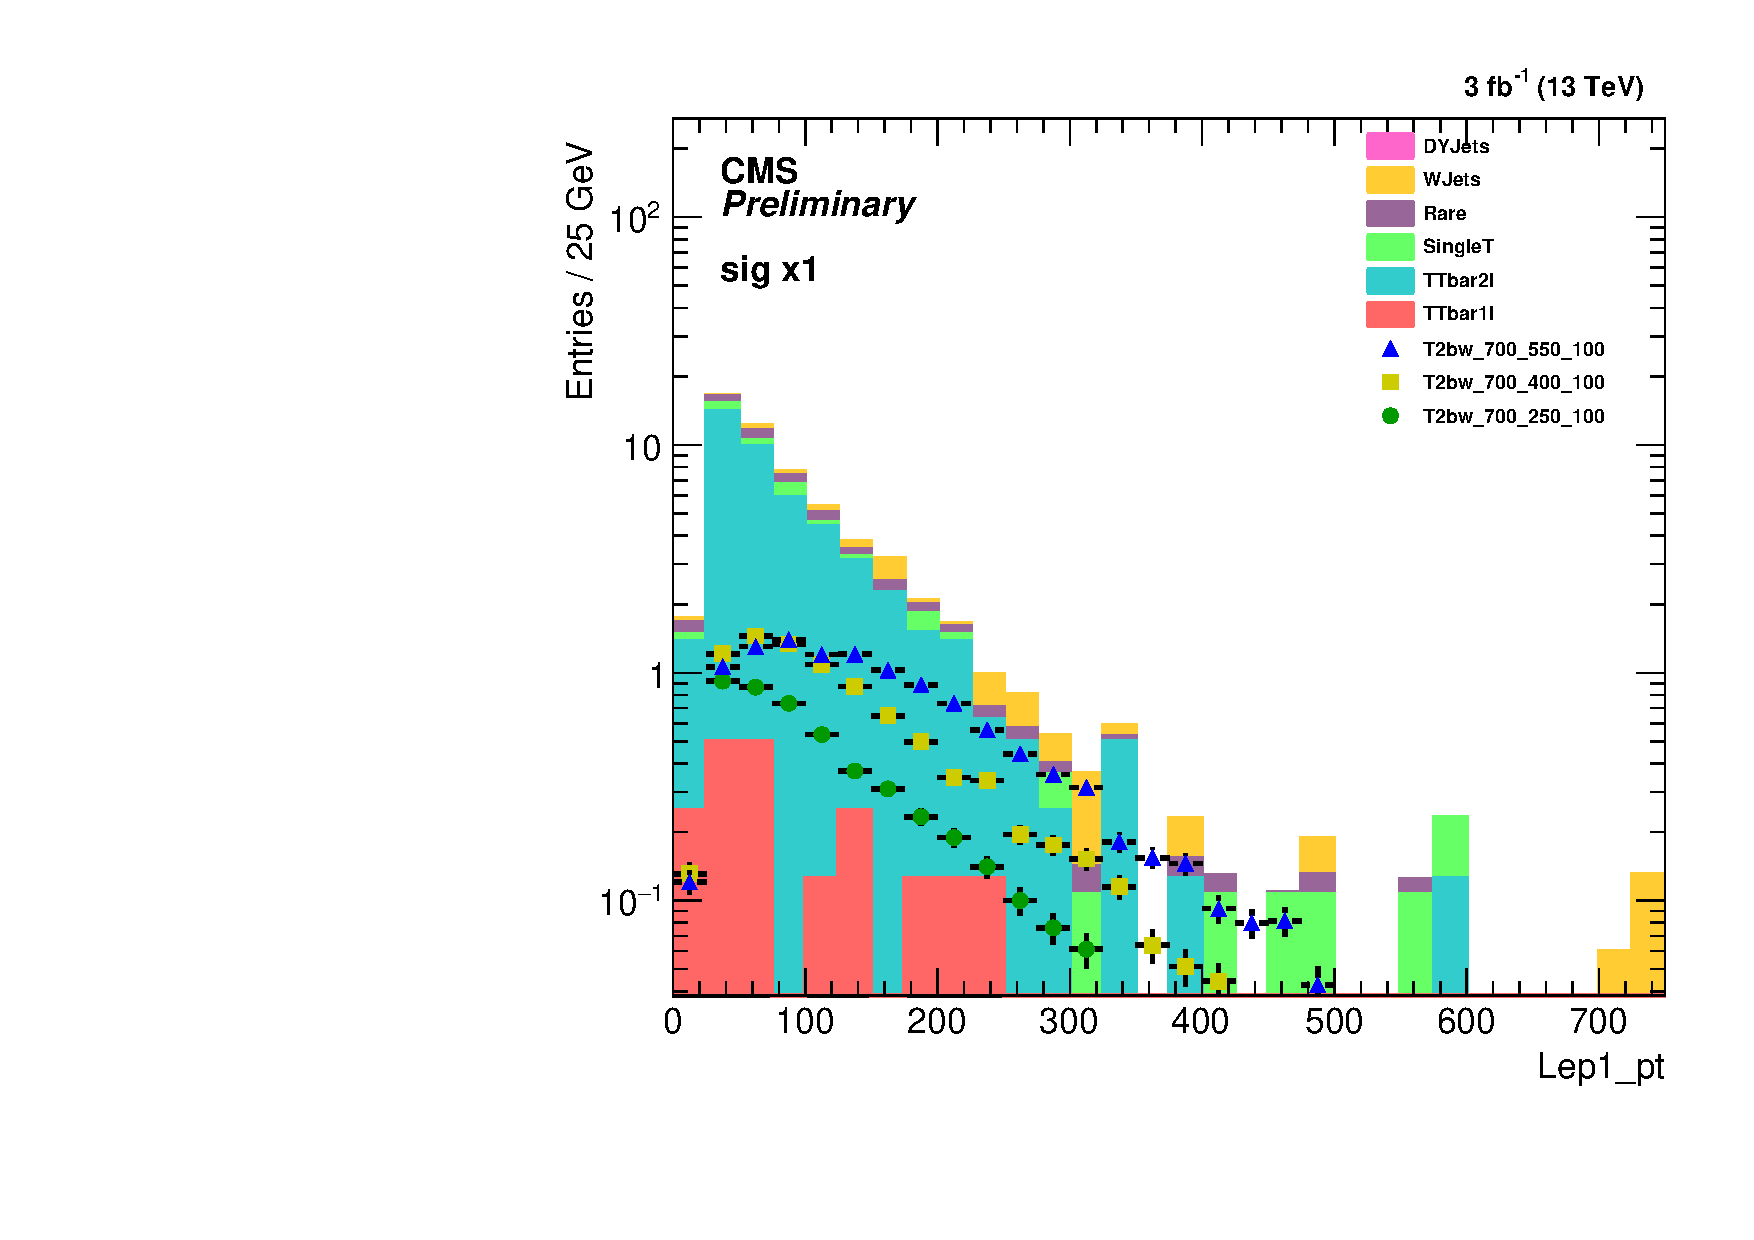
\includegraphics[width=0.49\textwidth]{Figures/SignalVariableStudies/Lep1_pt.pdf}
\label{fig:sigvarstudy:bptlpt:lpt}
}
\caption{\label{fig:sigvarstudy:bptlpt} Leading b-jet-\pt (left) and lepton-\pt (right) distributions.}
\end{figure}

\subsubsection{Lepton-\pt}

If the mass splitting between  the chargino and the LSP (in the top squark decay chain) is large, the lepton produced in the subsequent chargino can be very boosted, although the boost of the lepton depends on the momentum sharing between the lepton and neutrino of the \PW boson decay. Still, the lepton-\pt can enhance the signal discrimination, as it can be appreciated in fig.~\ref{fig:sigvarstudy:bptlpt:lpt}.

\subsubsection{$\MTt(\ell,\cPq\cPq)$}

Such a variable could be sensitive for the production of charginos as in $\PSQt\to\cPqb\PSGcpmDo$, $\PSGcpmDo\to\PW\PSGczDo$, as it should correlated with the mass splitting between the chargino and the LSP.

Figure~\ref{fig:sigvarstudy:MT2lqqHTfrac:MT2lqq} shows the $\MTt(\ell,\cPq\cPq)$ distribution. However, even for a T2bW like signature, no strong discrimination power was observed.

\begin{figure}
\subfigure[$\MTt(\ell,\cPq\cPq)$ distribution.]{
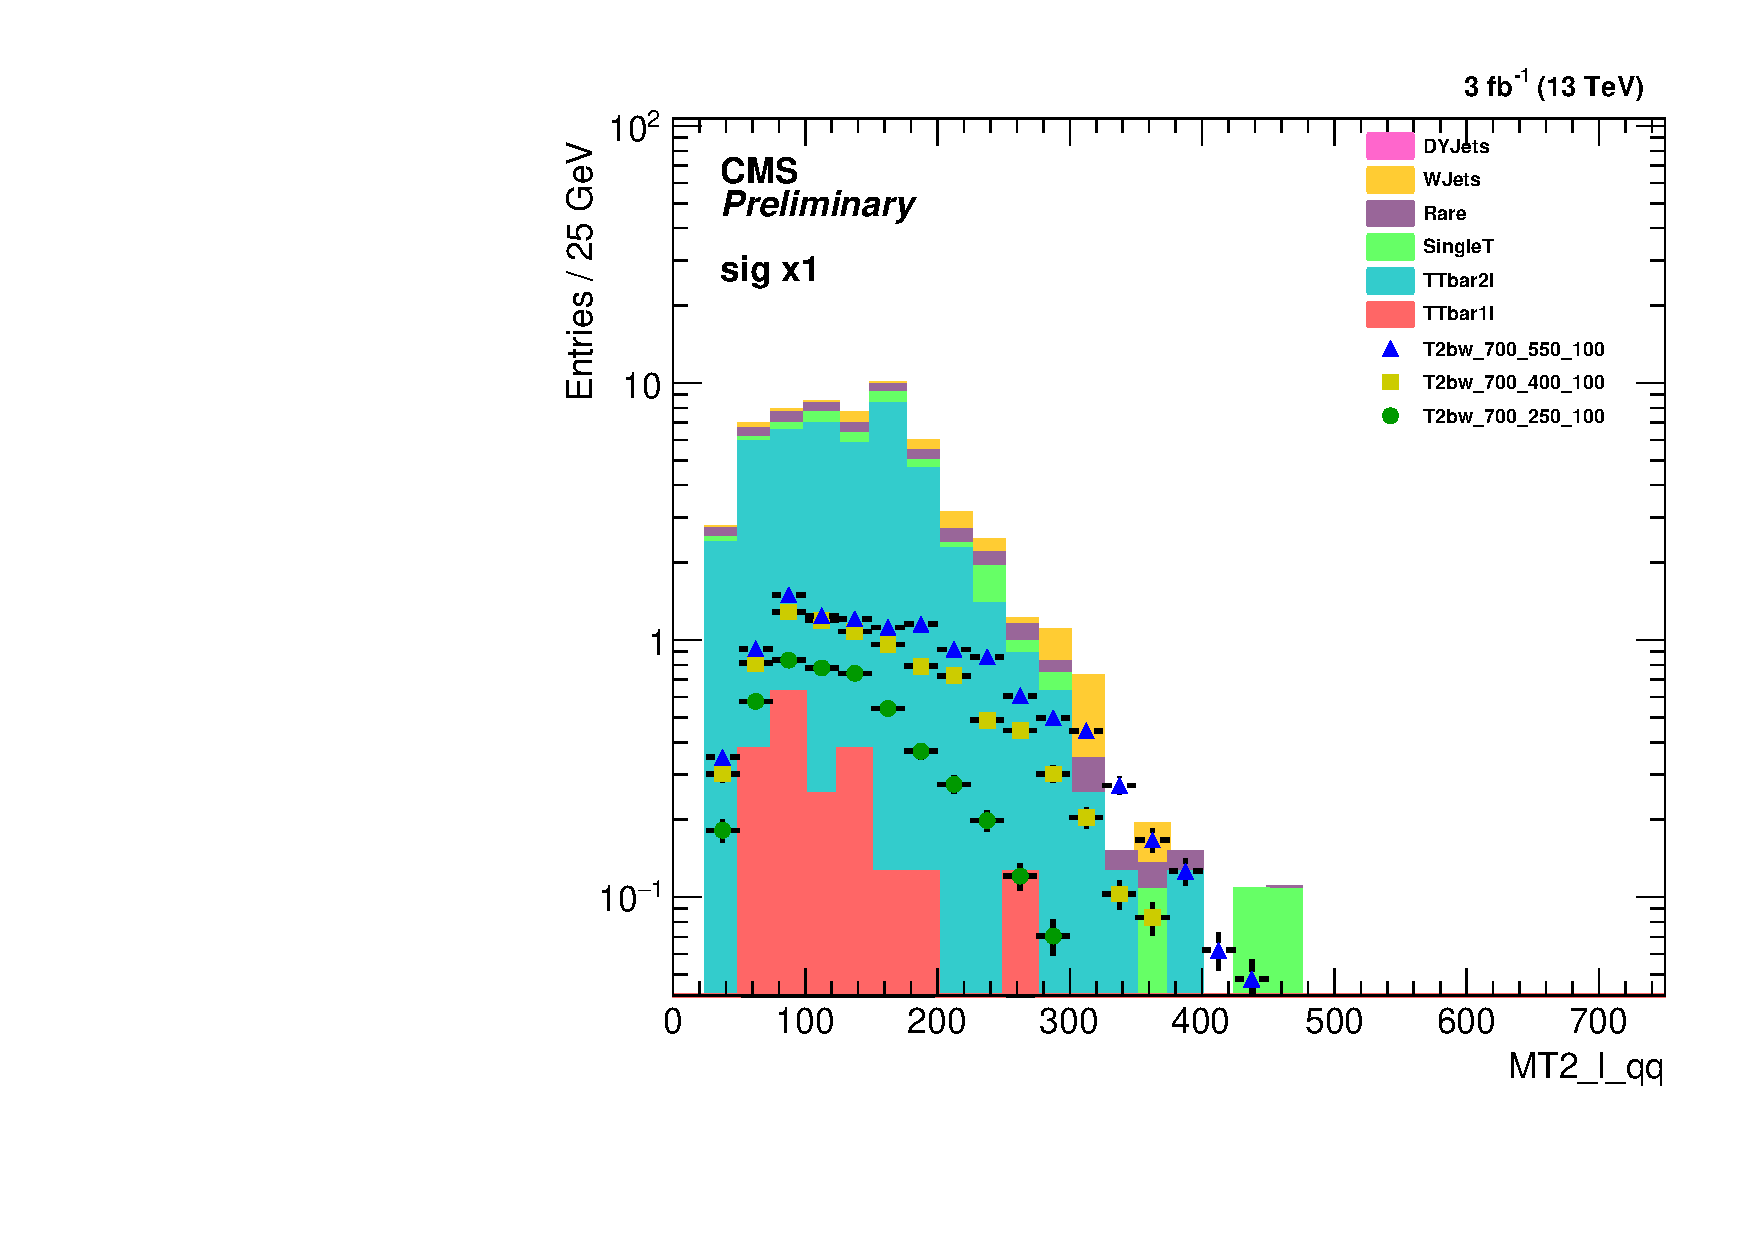
\includegraphics[width=0.49\textwidth]{Figures/SignalVariableStudies/MT2_l_qq_v2.pdf}
\label{fig:sigvarstudy:MT2lqqHTfrac:MT2lqq}
}
\subfigure[$\HT^\mathrm{frac}$ distribution.]{
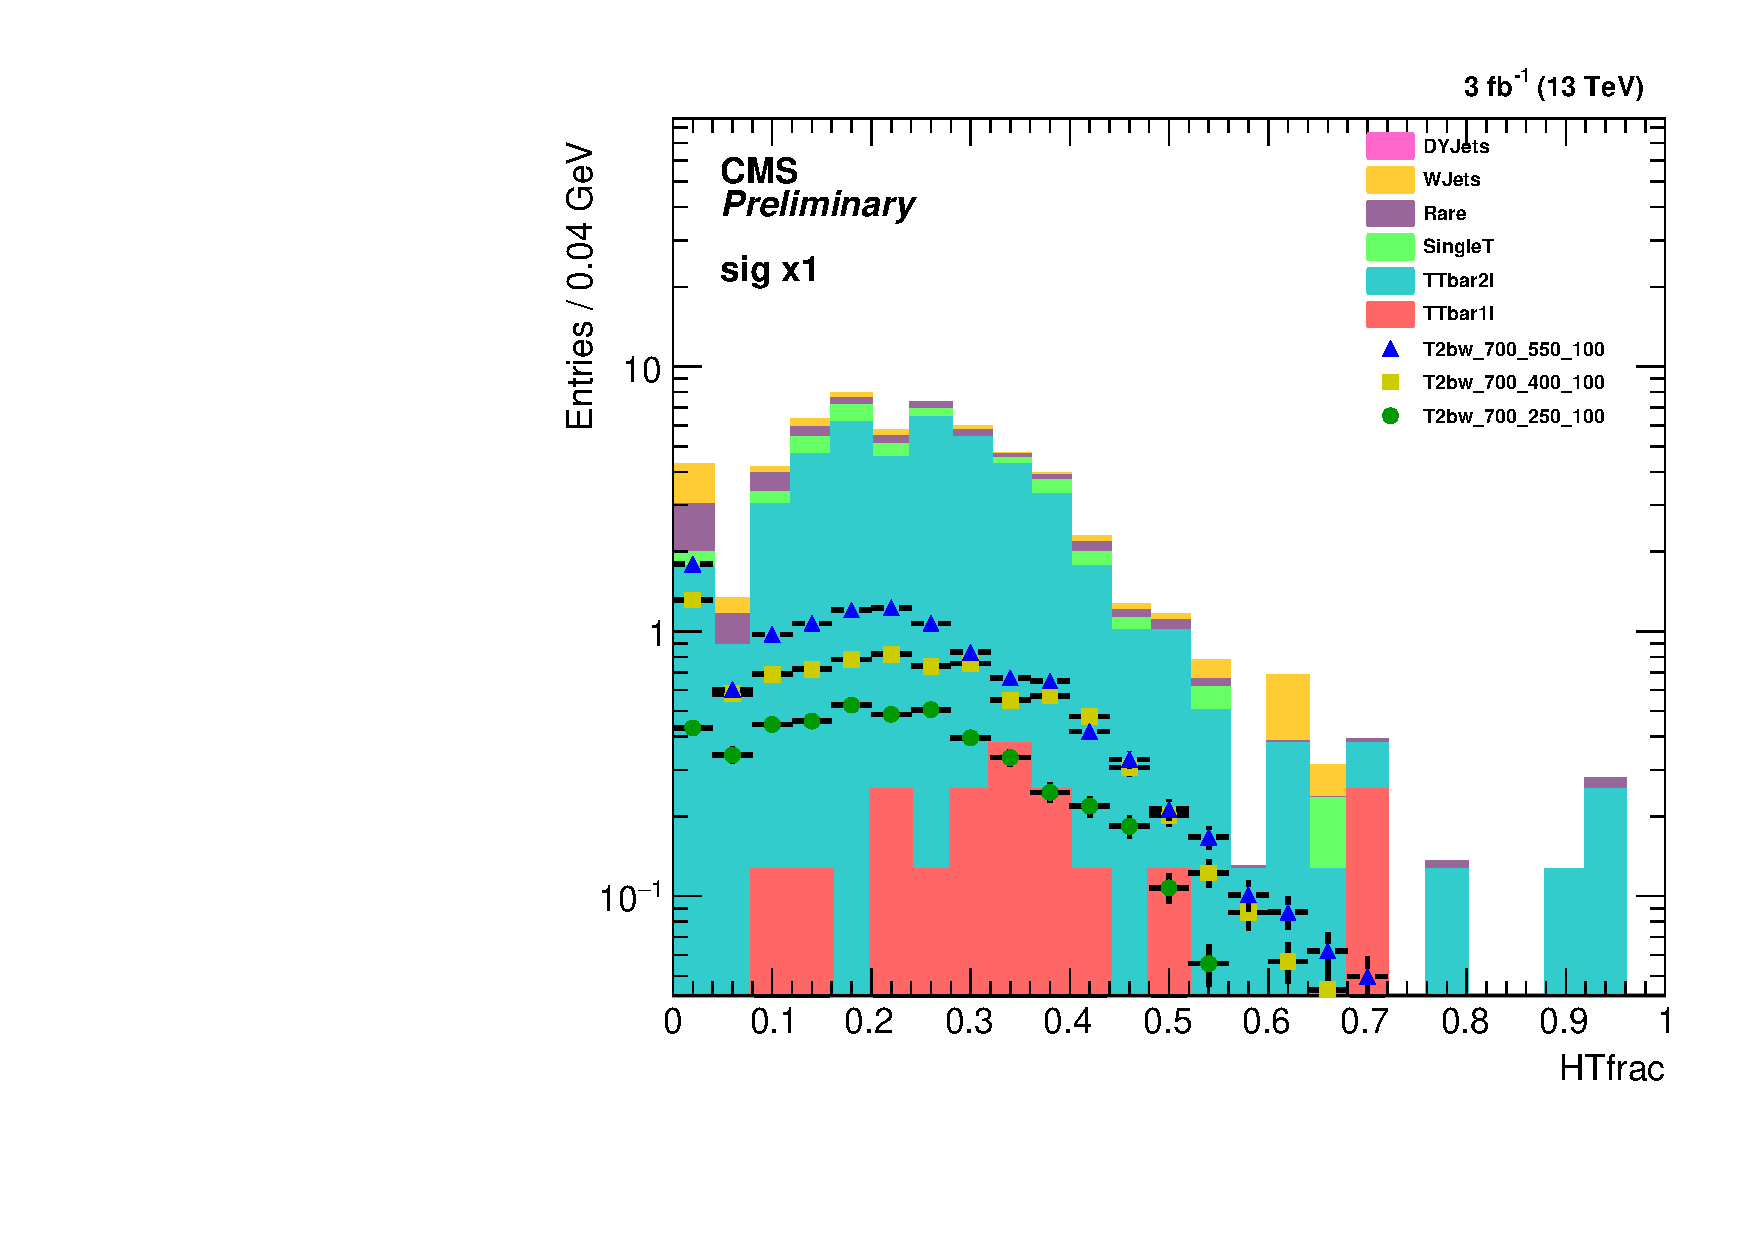
\includegraphics[width=0.49\textwidth]{Figures/SignalVariableStudies/HTfrac.pdf}
\label{fig:sigvarstudy:MT2lqqHTfrac:HTfrac}
}
\caption{\label{fig:sigvarstudy:MT2lqqHTfrac} $\MTt(\ell,\cPq\cPq)$ (left) and $\HT^\mathrm{frac}$ (right) distributions.}
\end{figure}

\subsubsection{$\HT^\mathrm{frac}$}

n the 8 TeV analysis~\cite{Chatrchyan:2013xna}, $\HT^\mathrm{frac}$ had been used in the event selection.
The corresponding distribution is shown in fig.~\ref{fig:sigvarstudy:MT2lqqHTfrac:HTfrac}. We clearly see, that the discrimination is very weak. Maybe, this variable could be used in a multivariate analysis.

\subsection{Evaluation of the signal variables}

From the variables studied, we found four main variables (besides \MET) that can enhance the signal--background discrimination: \MTtW, $M_{\ell \cPqb}$, the leading b-jet-\pt, and the lepton-\pt.

Already for 3\fbinv, we realized that for a ``cut-and-count'' analysis, the lepton-\pt is not suitable.
Also, adding two additonal variable selections on top of \MET and \MTtW is not feasible with 3\fbinv, although such a selection will be tempting with $\mathcal{O}(10\fbinv)$. However, that has to be studied.

Here, we summarize the study of adding either the leading b-jet-\pt or $M_{\ell \cPqb}$ to the selection, or even replacing \MTtW in the selection.
The procedure of the evalution was done as follows:
\begin{enumerate}
\item Define variables used. For \MTtW we chose a two-bin selection cutting at $\MTtW=200\GeV$, for $M_{\ell \cPqb}$ the value is at 175\GeV, while for the leading b-jet-\pt several options were investigated. It was found that cutting either at 100\GeV or 150\GeV are the best options for 3\fbinv.
\item Define a \MET binning for which we have $\gtrsim 2$ signal events in each bin at least one of the signal points.
\item Compute the signal sensitivity for all signals for that binning.
\item Get best ``averaged'' sensitivity for these signals. This last point is done subjectively, as we want to choose those signal regions that lead to good sensitivity for most of the signals, and avoid signal regions that lead to asymmetric sensitivities.
\end{enumerate}

With this procedure, 17 options were investigated. Following options seemed to be promising:
\begin{itemize}
\item v1: $\MTtW\lessgtr200\GeV$, up to 5 bins in \MET (8 bins)
\item v2: leading b-jet-$\pt \lessgtr 100\GeV$, $\MTtW\lessgtr200\GeV$, up to 4 bins in \MET (8 bins)
\item v3: leading b-jet-$b\pt \lessgtr 150\GeV$, $\MTtW\lessgtr200\GeV$, up to 3 bins in \MET (8 bins) 
\item v4: $M_{\ell \cPqb} \lessgtr 175\GeV$, $\MTtW\lessgtr200\GeV$, up to 3 bins in \MET (8 bins) 
\end{itemize}

The significances for all those options and all studies signal points is given in table~\ref{tab:sec:sigvarstudy:eval2}. For this table, all masses are given in GeV. Signals with $M(\PSQt_1) = 700\GeV$ have an LSP mass of 100 GeV, while signals with $M(\PSQt_1) = 600\GeV$ have an LSP mass of 50 GeV.

\begin{table}
\begin{center}
\caption{Significances for all those options and all studies signal points for 3\fbinv. All masses are given in GeV. Signals with $M(\PSQt_1) = 700\GeV$ have an LSP mass of 100 GeV, while signals with $M(\PSQt_1) = 600\GeV$ have an LSP mass of 50 GeV.\label{tab:sec:sigvarstudy:eval2}}
\tiny
%\setlength{\tabcolsep}{1pt}
%\scalebox{0.825}{
\begin{tabular}{|l|cccccc|ccc|cccc|}
\hline
signif & \multicolumn{6}{c|}{T2bW: $M(\PSQt_1)$-$M(\PSGcpmDo)$} & \multicolumn{3}{c|}{T2tb: $M(\PSQt_1)$-$M(\PSGcpmDo)$} & \multicolumn{4}{c|}{T2tt: : $M(\PSQt_1)$-$M(\PSGczDo)$} \\
   & 600-187.5 & 600-325 & 600-462.5 & 700-250 & 700-400 & 700-550 & 700-250 & 700-400 & 700-550 & 425-325 & 500-325 & 650-325 & 850-100 \\
\hline
v1 & 1.14 & 2.21 & 3.08 & 0.93 & 1.67 & 2.03 & 1.76 & 2.03 & 2.21 & 0.57 & 0.69 & 1.38 & 1.03\\ 
v2 & 1.29 & 2.32 & 3.06 & 1.00 & 1.72 & 1.99 & 1.71 & 1.99 & 2.12 & 0.52 & 0.57 & 1.38 & 0.94 \\
v3 & 1.35 & 2.32 & 3.09 & 1.08 & 1.79 & 2.04 & 1.79 & 2.05 & 2.19 & 0.48 & 0.54 & 1.39 & 0.98 \\
v4 & 1.34 & 2.35 & 3.14 & 1.08 & 1.83 & 2.13 & 1.73 & 2.01 & 2.15 & 0.54 & 0.66 & 1.41 & 0.95 \\
\hline
\end{tabular}
%}
\end{center}
\end{table}

For the assumption of 3\fbinv, the option v4 seemed overall most promising. The binning for that option as well as background and signal yields are given in tables~\ref{tab:sec:sigvarstudy:SR2} and~\ref{tab:sec:sigvarstudy:yields2}.

\begin{table}
\begin{center}
\caption{Binning for ``optimal'' signal regions of a ``cut-and-count'' analysis under the assumption of 3\fbinv. \label{tab:sec:sigvarstudy:SR2}}
%\tiny
%\setlength{\tabcolsep}{1pt}
\begin{tabular}{|l|l|ccc|}
\hline
$M_{\ell \cPqb}$ [GeV] & $\MTtW$ [GeV] & \multicolumn{3}{c|}{\MET [GeV]} \\
\hline
$\leq 175$ & $\leq 200$ & $250-325$ & $>325$ & \\
$\leq 175$ & $> 200$ & $250-375$ & $>375$ & \\
$> 175$ & $\leq 200$ & $>250$ & & \\
$> 175$ & $> 200$ & $250-300$ & $300-400$ & $>400$ \\
\hline
\end{tabular}
\end{center}
\end{table}
\begin{table}
\begin{center}
\caption{Signal and background yields for ``optimal'' signal regions of a ``cut-and-count'' analysis under the assumption of 3\fbinv. All masses are given in GeV. Signals with $M(\PSQt_1) = 700\GeV$ have an LSP mass of 100 GeV, while signals with $M(\PSQt_1) = 600\GeV$ have an LSP mass of 50 GeV.\label{tab:sec:sigvarstudy:yields2}}
\tiny
%\setlength{\tabcolsep}{1pt}
%\scalebox{1.0}{
\begin{tabular}{|l|c|cccccc|ccc|cccc|}
\hline
 \MET [$\geq$GeV] & bg & \multicolumn{6}{c|}{T2bW: $M(\PSQt_1)$-$M(\PSGcpmDo)$} & \multicolumn{3}{c|}{T2tb: $M(\PSQt_1)$-$M(\PSGcpmDo)$} & \multicolumn{4}{c|}{T2tt: : $M(\PSQt_1)$-$M(\PSGczDo)$} \\
 & & 600-187.5 & 600-325 & 600-462.5 & 700-250 & 700-400 & 700-550 & 700-250 & 700-400 & 700-550 & 425-325 & 500-325 & 650-325 & 850-100 \\
\hline
 & & \multicolumn{13}{l|}{$M_{\ell \cPqb}\leq175\GeV$, $\MTtW\leq200\GeV$} \\
\hline
 $250-325$    & 23.3$\pm$1.7 & 0.4$\pm$0.0 & 0.9$\pm$0.1 & 2.2$\pm$0.1 & 0.2$\pm$0.0 & 0.4$\pm$0.0 & 0.8$\pm$0.0 & 0.6$\pm$0.0 & 0.6$\pm$0.0 & 0.9$\pm$0.0 & 0.8$\pm$0.1 & 1.7$\pm$0.2 & 1.9$\pm$0.1 & 0.2$\pm$0.0 \\
 $325-\infty$ & 11.4$\pm$1.2 & 0.3$\pm$0.0 & 0.8$\pm$0.1 & 2.5$\pm$0.1 & 0.3$\pm$0.0 & 0.5$\pm$0.0 & 1.2$\pm$0.0 & 1.0$\pm$0.0 & 1.1$\pm$0.0 & 1.6$\pm$0.1 & 1.5$\pm$0.1 & 2.5$\pm$0.2 & 1.8$\pm$0.1 & 0.5$\pm$0.0 \\
\hline
 & & \multicolumn{13}{l|}{$M_{\ell \cPqb}\leq175\GeV$, $\MTtW>200\GeV$} \\
\hline
 $250-375$    & 5.5$\pm$0.8 & 0.7$\pm$0.1 & 1.8$\pm$0.1 & 2.7$\pm$0.1 & 0.4$\pm$0.0 & 0.9$\pm$0.0 & 1.1$\pm$0.0 & 1.1$\pm$0.0 & 1.4$\pm$0.1 & 1.4$\pm$0.1 & 0.3$\pm$0.0 & 0.3$\pm$0.1 & 2.4$\pm$0.1 & 0.4$\pm$0.0 \\
 $375-\infty$ & 2.9$\pm$0.6 & 0.4$\pm$0.0 & 1.3$\pm$0.1 & 2.6$\pm$0.1 & 0.4$\pm$0.0 & 1.0$\pm$0.0 & 1.6$\pm$0.1 & 2.1$\pm$0.1 & 2.3$\pm$0.1 & 2.7$\pm$0.1 & 0.4$\pm$0.0 & 0.3$\pm$0.1 & 1.8$\pm$0.1 & 1.5$\pm$0.0 \\
\hline
 & & \multicolumn{13}{l|}{$M_{\ell \cPqb}>175\GeV$, $\MTtW\leq200\GeV$} \\
\hline
 $250-\infty$ & 7.5$\pm$1.0 & 0.3$\pm$0.0 & 0.6$\pm$0.1 & 2.0$\pm$0.1 & 0.2$\pm$0.0 & 0.5$\pm$0.0 & 0.9$\pm$0.0 & 0.4$\pm$0.0 & 0.4$\pm$0.0 & 0.7$\pm$0.0 & 0.3$\pm$0.0 & 0.6$\pm$0.1 & 0.5$\pm$0.0 & 0.1$\pm$0.0 \\
\hline
 & & \multicolumn{13}{l|}{$M_{\ell \cPqb}>175\GeV$, $\MTtW>200\GeV$} \\
\hline
 $250-300$    & 2.5$\pm$0.5 & 1.7$\pm$0.1 & 2.3$\pm$0.1 & 2.4$\pm$0.1 & 0.9$\pm$0.0 & 1.4$\pm$0.1 & 1.2$\pm$0.0 & 0.8$\pm$0.0 & 0.9$\pm$0.0 & 0.8$\pm$0.0 & 0.1$\pm$0.0 & 0.2$\pm$0.0 & 0.5$\pm$0.0 & 0.1$\pm$0.0 \\
 $300-400$    & 3.7$\pm$0.6 & 1.7$\pm$0.1 & 3.2$\pm$0.1 & 4.0$\pm$0.1 & 1.4$\pm$0.1 & 2.2$\pm$0.1 & 2.2$\pm$0.1 & 1.4$\pm$0.1 & 1.8$\pm$0.1 & 1.7$\pm$0.1 & 0.4$\pm$0.0 & 0.1$\pm$0.0 & 0.6$\pm$0.0 & 0.3$\pm$0.0 \\
 $400-\infty$ & 2.0$\pm$0.5 & 0.8$\pm$0.1 & 1.9$\pm$0.1 & 2.8$\pm$0.1 & 1.0$\pm$0.0 & 2.0$\pm$0.1 & 2.6$\pm$0.1 & 1.7$\pm$0.1 & 2.1$\pm$0.1 & 2.3$\pm$0.1 & 0.4$\pm$0.0 & 0.2$\pm$0.1 & 0.6$\pm$0.0 & 0.8$\pm$0.0 \\
 \hline
\end{tabular}
%}
\end{center}
\end{table}

As the final dataset size of all the pp collision data collected by the CMS experiment in 2015 was lower than 3\fbinv, the re-evaluation showed, that we cannot keep a selection based on \MET, \MTtW, and $M_{\ell \cPqb}$. This re-evaluation led to the signal regions defined in section~\ref{sec:obj_sel:signal_regions}.

%\section{MT Studies}
\label{sec:MTstudies}
The signal events in this analysis populate the tails of the M$_{T}(\MET,lep)$ distribution ($>120$).  A study was conducted to evaluate the modeling of the MT tails in simulation.  This study consisted of data MC comparisons in several W+Jets control regions with selections close to those in our signal region.
\begin{itemize}
\item nJets $\ge$ 2 (Jet pt>30 GeV, |$\eta$|<2.4, Loose PFId, remove overlaps)
\item 0 btagged jets (with medium pfCombinedInclusiveSecondaryVertexV2BJetTags)
\item 1 good lepton: pT>35 GeV, |$\eta$|<2.1, medium POG ID (no iso), miniRelIso<0.1, (for muons dz=0.1, and d0=0.02)
\item 2nd reconstructed lepton veto: electron (Veto POG ID, pT>5 GeV, |$\eta$|<2.4, miniRelIso<0.2) or muon (loose POG ID, pT>5 GeV, |$\eta$|<2.4, d0<0.1 cm, dz<0.5 cm, miniRelIso<0.2)
\item pfMET>50,100,150 GeV (type1 corrected)
\item Pass unprescaled single-lepton triggers, also used for the analysis.
In addition, noise filters were applied on data to remove events with fake \MET emerging from calorimeter noise or beam halo.  
The tails of MT are sensitive to events with significant fake \MET.  To remove thse events, noise filters were applied on data to remove events with fake \MET emerging from calorimeter noise or beam halo.  The filters recommended by the JetMET POG:
\begin{itemize}
\item primary vertex filter
\item CSC beam halo filter
\item HBHE noise filter
\item HBHE iso noise filter
\item ee badSC noise filter
\end{itemize}
were applied to data for the MT studies and for the main analysis.  They were found to have a $<2\%$ impact on the yield.

\begin{figure}[h]
\includegraphics[width=0.95\textwidth]{Figures/bkg1lep/MT_MET50.png}
\includegraphics[width=0.95\textwidth]{Figures/bkg1lep/MT_MET150.png}
\caption{\label{fig:MTComissioning} MT distributions with 1.6 fb$^{-1}$ for muon, barrel electrons, and endcap electron events with MET$>50$ (top) and MET$>150$ (bottom)}
\end{figure}

The MT distributions for \MET$>50$ and \MET$\>100$ GeV are shown on Figure~\ref{fig:MTCommissioning}.  Good agreement between data and MC for events with muons and barrel electron was shown in both the MT bulk region(60$<$MT$<$120) and the MT tail (MT$>$120).  There is also good agreement between data and MC for events with endcap electrons in the bulk of the MT spectrum.  However, a large data excess of endcap electron events with large MT values was also observed.  As can be seen from these figures, the MT tail of the endcap electrons is greatly reduced by the higher \MET cut.  However, it does not completely disappear.  With the limited statistics available, it is not possible to determine if this excess persists after \MET$>250$ were the signal regions for this analysis begin.  The excess was found to be correlated to electron pT, Figure~\ref{fig:MTepT2D}.  Further studies on the isolation distributions of events with MT$>120$ suggested that this excess is from fake electrons, Figure~\ref{fig:minireliso}.

\begin{figure}[h]
\includegraphics[width=0.95\textwidth]{Figures/bkg1lep/MT_Elpt_data.pdf}
\caption{\label{fig:MTepT2D} M$_{T}$(\MET,e) v. electron pT for endcap electron events shows a strong correlation betweeen MT and electron pT}
\end{figure}
\begin{figure}[h]
\includegraphics[width=0.95\textwidth]{Figures/bkg1lep/EndcapEl_miniRelIsopdf}
\caption{\label{fig:minireliso} MiniRelIso distribution for endcap electrons with MT$>120$ indicates that the excess in data is from fakes}
\end{figure}
\begin{figure}[h]
\includegraphics[width=0.95\textwidth]{Figures/bkg1lep/MT_MET150_2p11.png}
\caption{\label{fig:MTComissioning} MT distributions with 2.11 fb$^{-1}$ for muon, barrel electrons, and endcap electron events with MET$>150$ (bottom)}
\end{figure}
Applying tighter ID and isolation requirements was explored but it was determined that due to the poor modeling of these events, even a tight isolation cut would not make a significant difference.  Furthermore,  tighter isolation would significantly reduce signal acceptance.  Since the signal acceptance of the leptons tends to be central, removing events with endcap electrons from this analysis was a more suitable option.  

These studies were done with 1.6 fb$^{-1}$ and again repeated for the full 2.11$fb^{-1}$.  The MT distributions for the full dataset was shown on Figure~\ref{fig:MTFinal}.   We will continue comissioning of the MT tails for the full 13 TeV dataset.


\section{Studies on Reducing the Lost Lepton Background}
\label{sec:lost_lepton_studies}

This appendix discusses investigations on the suppresion of the diLepton background in the signal regions.  The process involves first understanding the kinematics of the lost leptons, then for those within the selection acceptance, optimizing the kinematic and isolation values used to reject these events without cutting out too much signal.  The starting point for these studies comes from the vetoes used in the 8 TeV analysis for this search.  


\subsection{Baseline Selection for Lost Lepton Studies}
\label{sec:lost_lepton_studies:baseline_selection}

\begin{itemize}
\item First vertex is good.
\item Exactly one selection lepton:
	\begin{itemize}
	\item Electrons: $\pt>40\GeV$, $|\eta|<2.1$, medium ID, miniiso$ < 0.1$,
	\item Muons: $\pt>30\GeV$, $|\eta|<2.1$, medium ID, miniiso$ < 0.2$,
	\end{itemize}
\item  At least four jets ($\pt>30\GeV$, $|\eta|<2.4$, loose ID),
\item  At least on b-jet (medium CSVv2+IVF WP),
\item  $\MET>200\GeV$ (type-1 corrected),
\item  $\MT>150\GeV$,
\item  $\minDPhiMETjet>0.8$.
\end{itemize}

For this study, PHYS14 simulation was used. The signal mass points are:
\begin{itemize}
\item $M_{\PSQt} = 500\GeV$, $M_{\PSGczDo} = 325\GeV$,
\item $M_{\PSQt} = 650\GeV$, $M_{\PSGczDo} = 325\GeV$,
\item $M_{\PSQt} = 850\GeV$, $M_{\PSGczDo} = 100\GeV$.
\end{itemize}

The background used for optimization was $t\bar{t}{\rightarrow}\ell\ell$, also a PHYS14 simulation.  

\subsection{The starting point: 8 TeV Lost Lepton Vetos}
\label{sec:lost_lepton_studies:8TeV}

The 8 TeV lost lepton veto identified charged pfCandidates, with low relative track isolation, and pfTau candidates that have been identified with an MVA ID.  Events were vetoed if the following criteria were met:

\begin{itemize}
  \item charged pfCandidates
    \begin{itemize}
       \item pfMuons, pfElectrons
         \begin{itemize}
           \item $p_{T}>5$ GeV
           \item $\eta<2.4$
           \item relative track isolation $<$ 0.2
         \end{itemize}
       \item pfChargedHadrons
         \begin{itemize}
            \item $p_{T}>10$ GeV
            \item $\eta<2.4$
            \item relative track isolation $<$ 0.1
            \item opposite sign charge as selected lepton
         \end{itemize}
    \end{itemize}
  \item pfTau candidates
    \begin{itemize}
      \item $p_{T}>20$ GeV
      \item $\eta<2.4$
      \item opposite sign charge as selected lepton
      \item MVA based ID     
    \end{itemize}
\end{itemize}


\subsection{Lost Lepton Classification and Kinematics}
\label{sec:lost_lepton_studies:classification}

At 13 TeV, the kinematics and isolation values of the pfCharged Candidates are expected to be slightly different, so it is necessary to study the lost lepton characteristics, at this collision energy, in order to optimize the veto selection. 

In order to identify a lost lepton, one looks for a gen-level lepton and matches it to its corresponding flavour, reconstructed pfCandidate.  For electrons, in an inclusive selection of $t\bar{t}$ events, the matching efficiency drops quickly for decreasing $p_{T}$, as shown in figure \ref{fig:lost_lepton_studies:el_gen_matching_eff}.  The lost lepton vetoes will be less efficient at low $p_{T}$, where the bulk of the lost lepton events, making it through the single lepton selection are distributed.  Thus, optimizing the cuts in the low lost lepton $p_{T}$ region will have the largest impact on background rejection.  

\begin{figure}[ht]
\centering
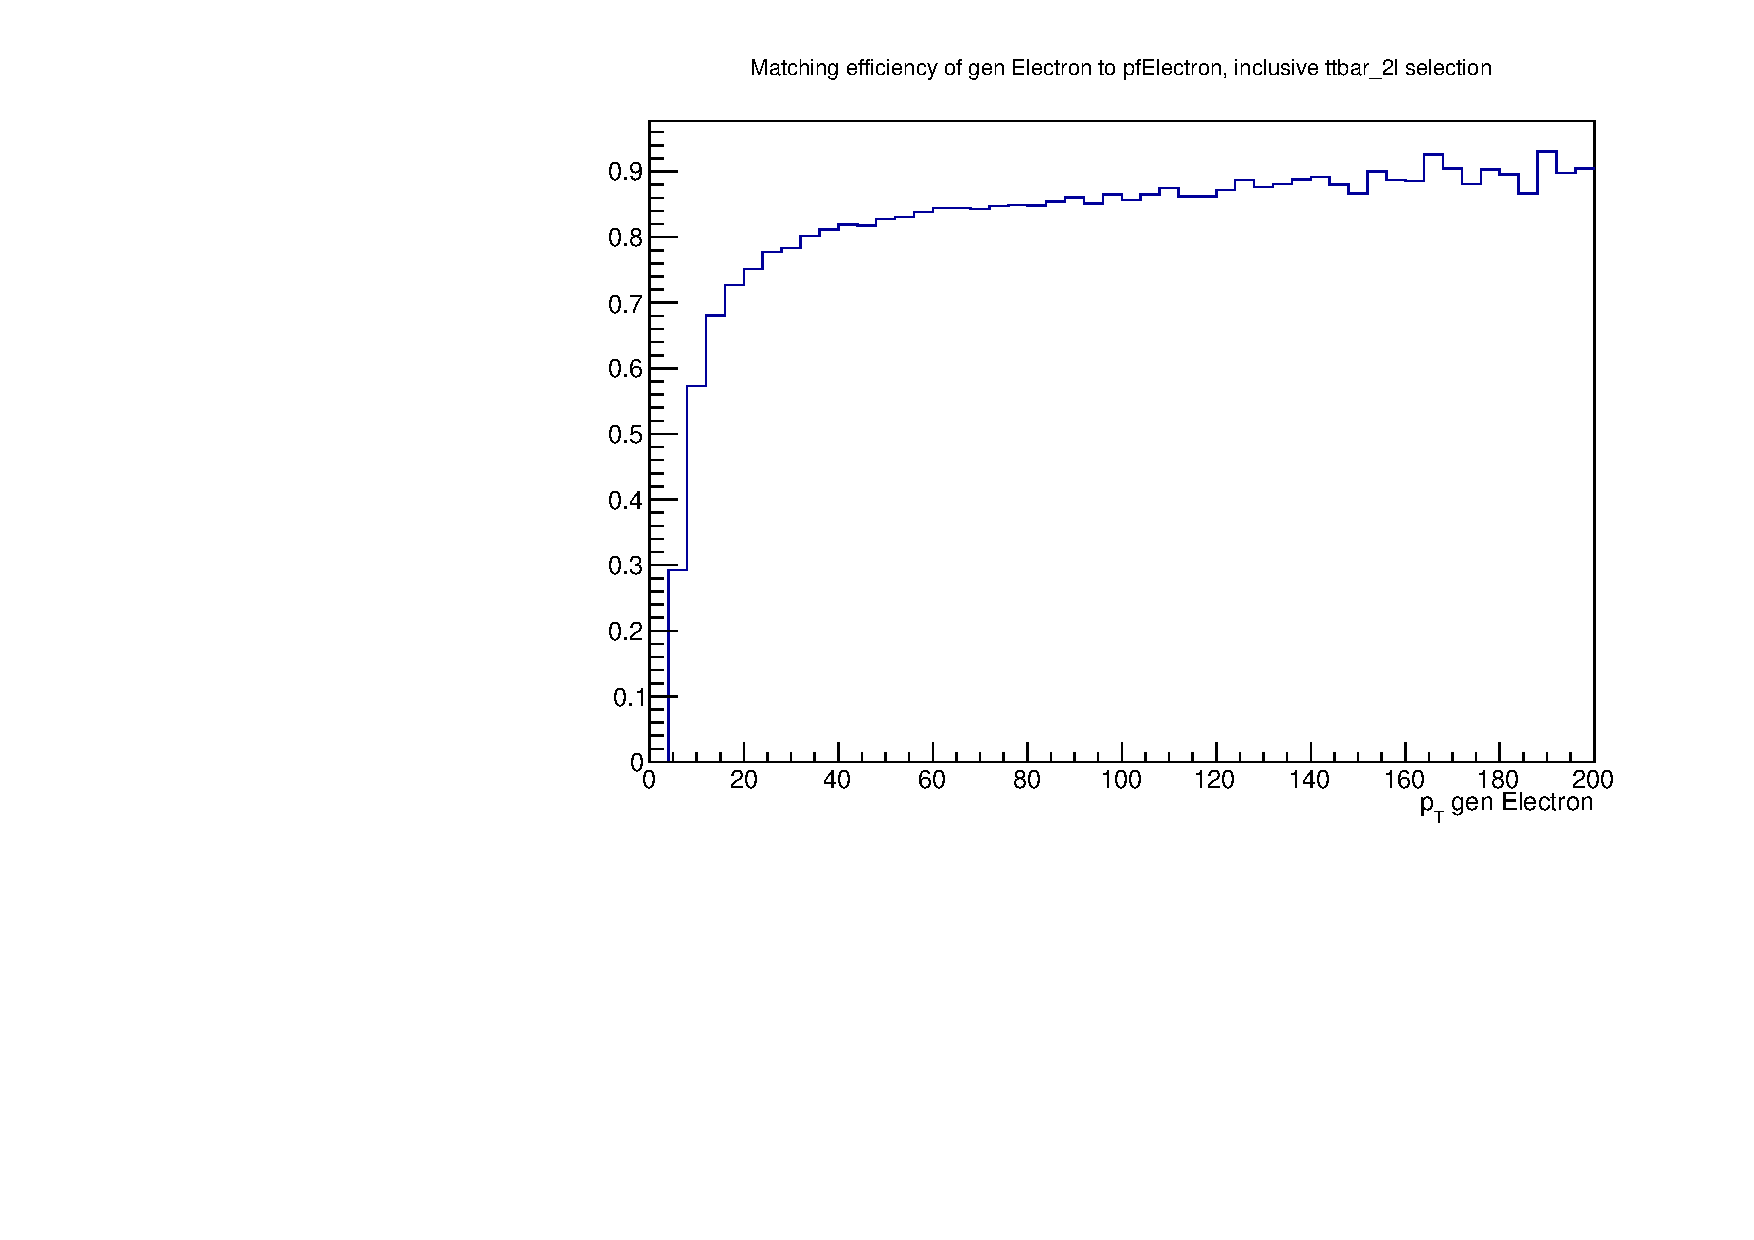
\includegraphics[width=0.60\textwidth]{Figures/studiesLostLepton/matchEff_genEl_to_pfEl_incl.pdf}
\caption{\label{fig:lost_lepton_studies:el_gen_matching_eff} Matching effiency vs $p_{T}$ between gen electrons and pfElectron candidates. }
\end{figure}

Approximately half of the lost leptons that pass the analysis selection are hadronically decaying taus, as shown in figure \ref{fig:lost_lepton_studies:classification}.  Of this 50\%, approximately 70\% of the hadronic tau decays are 1-prong, with the remaining approximately 30\% come from 3-prong decays.  Out of the lost electrons and muons, 8\% and 9\% of total lost leptons come from taus decaying to muons and leptons respectively.  Direct lost electrons compose approximately 17.5\% of the background, while director muons contribute approximately 14\%.  Since the leptons coming from tau decays will be softer in $p_{T}$ when compared to their direct counterparts, these will often fall out of acceptance and will difficult to tune cuts further in order to reject these events.  The largest impact in the analysis will come from reducing the 1-prong hadronically decaying taus.  Since these decays, by definition, will have a single isolated track, the use of tracker-baed isolation will be the best kinematic handle on reducing this background.  Since direct lepton decays also tend to be isolated, tracker isolation will also be used to target this background.  The 3-prong hadronic tau decays will be targeted using the MVA id.  

\begin{figure}[ht]
\centering
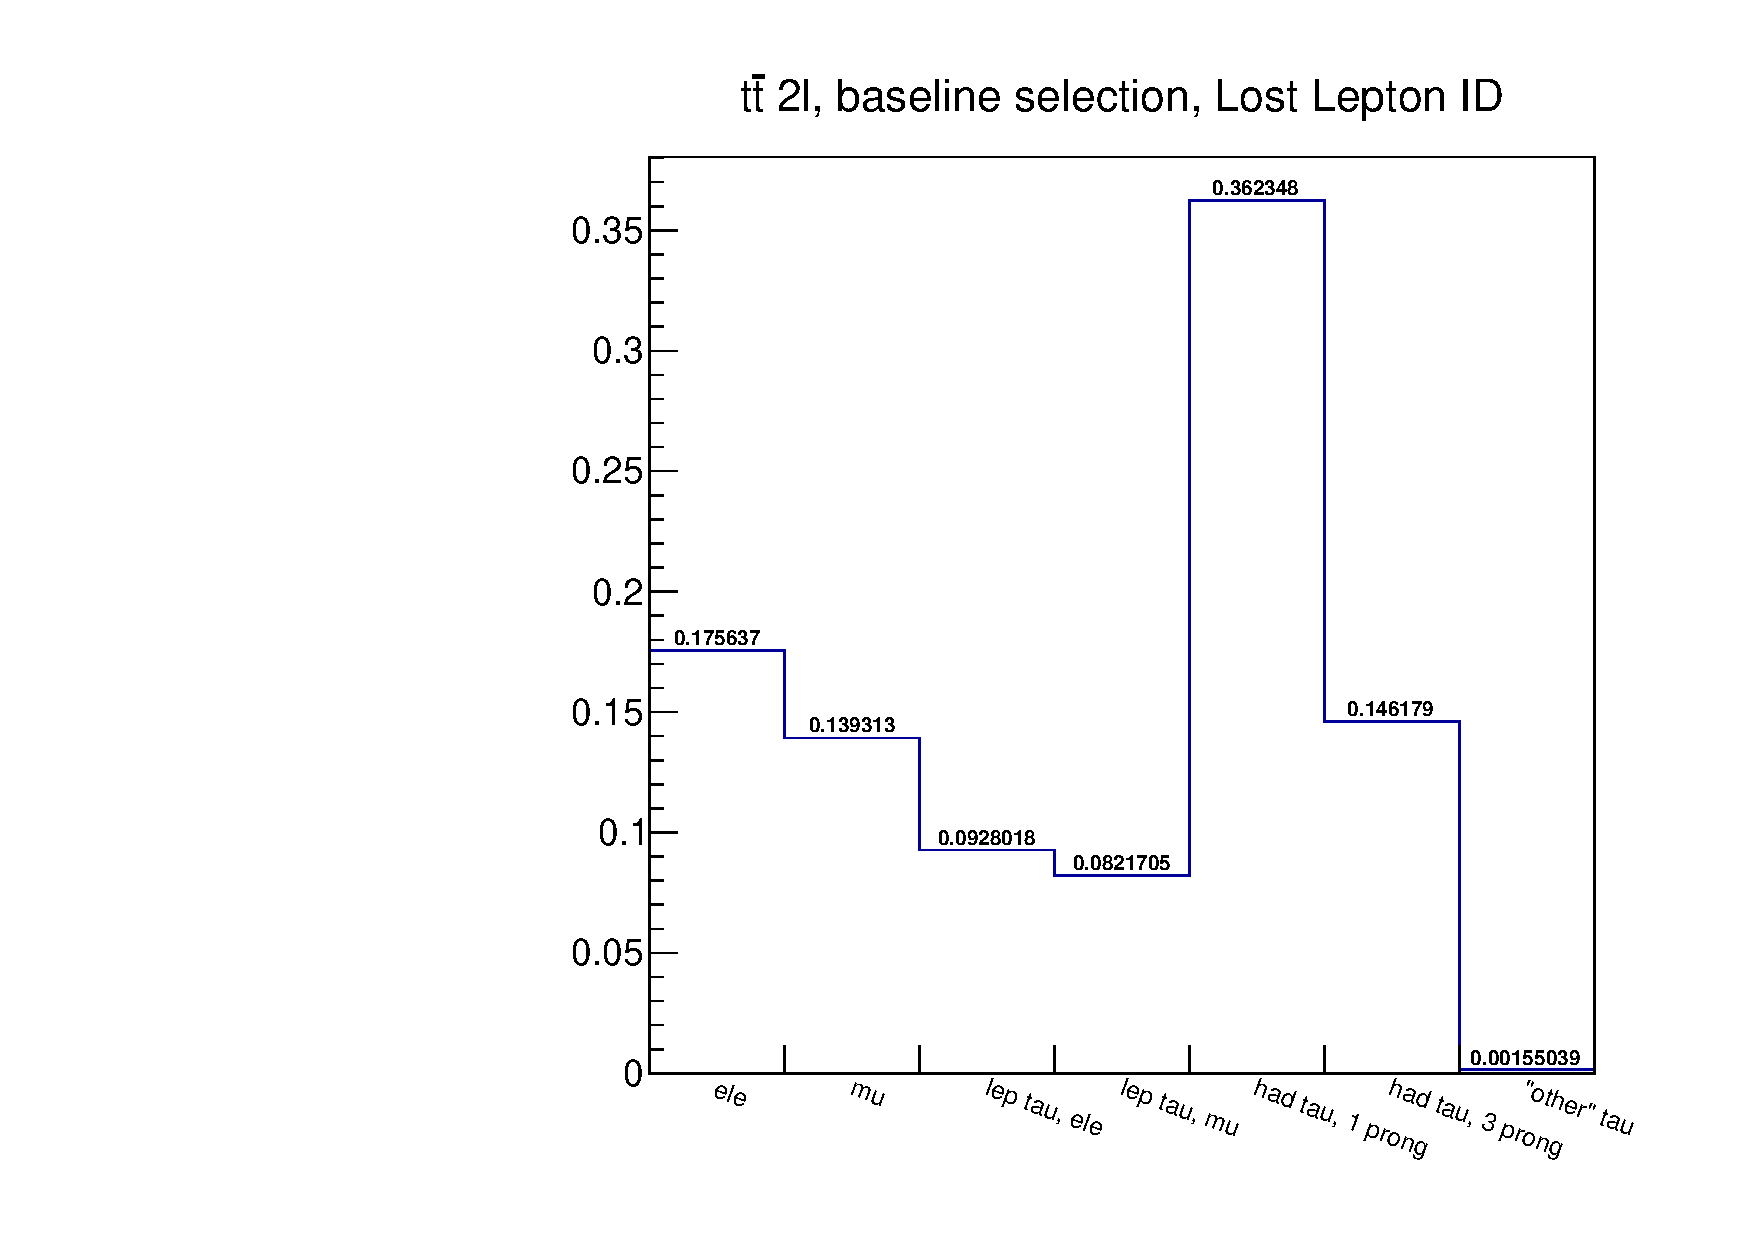
\includegraphics[width=0.60\textwidth]{Figures/studiesLostLepton/lostLeptonStudies__ttbar2l__lostLeptonID.pdf}
\caption{\label{fig:lost_lepton_studies:classification} Classification of the lost lepton flavour passing analysis selection }
\end{figure}

Next, it is important to understand the acceptance of these lost lepton events.  The majority of electron events, that fail acceptance, are from low pT.  Figure \ref{fig:lost_lepton_studies:el_acceptance} shows the $p_{T}$ and $\eta$ distrubtions for the lost gen electrons, including those coming from leptonic tau decays. Approximately 57\% of lost gen electrons pass the $p_{T}>5$GeV and $\eta<2.4$ cuts for the acceptance.    

\begin{figure}[ht]
\centering
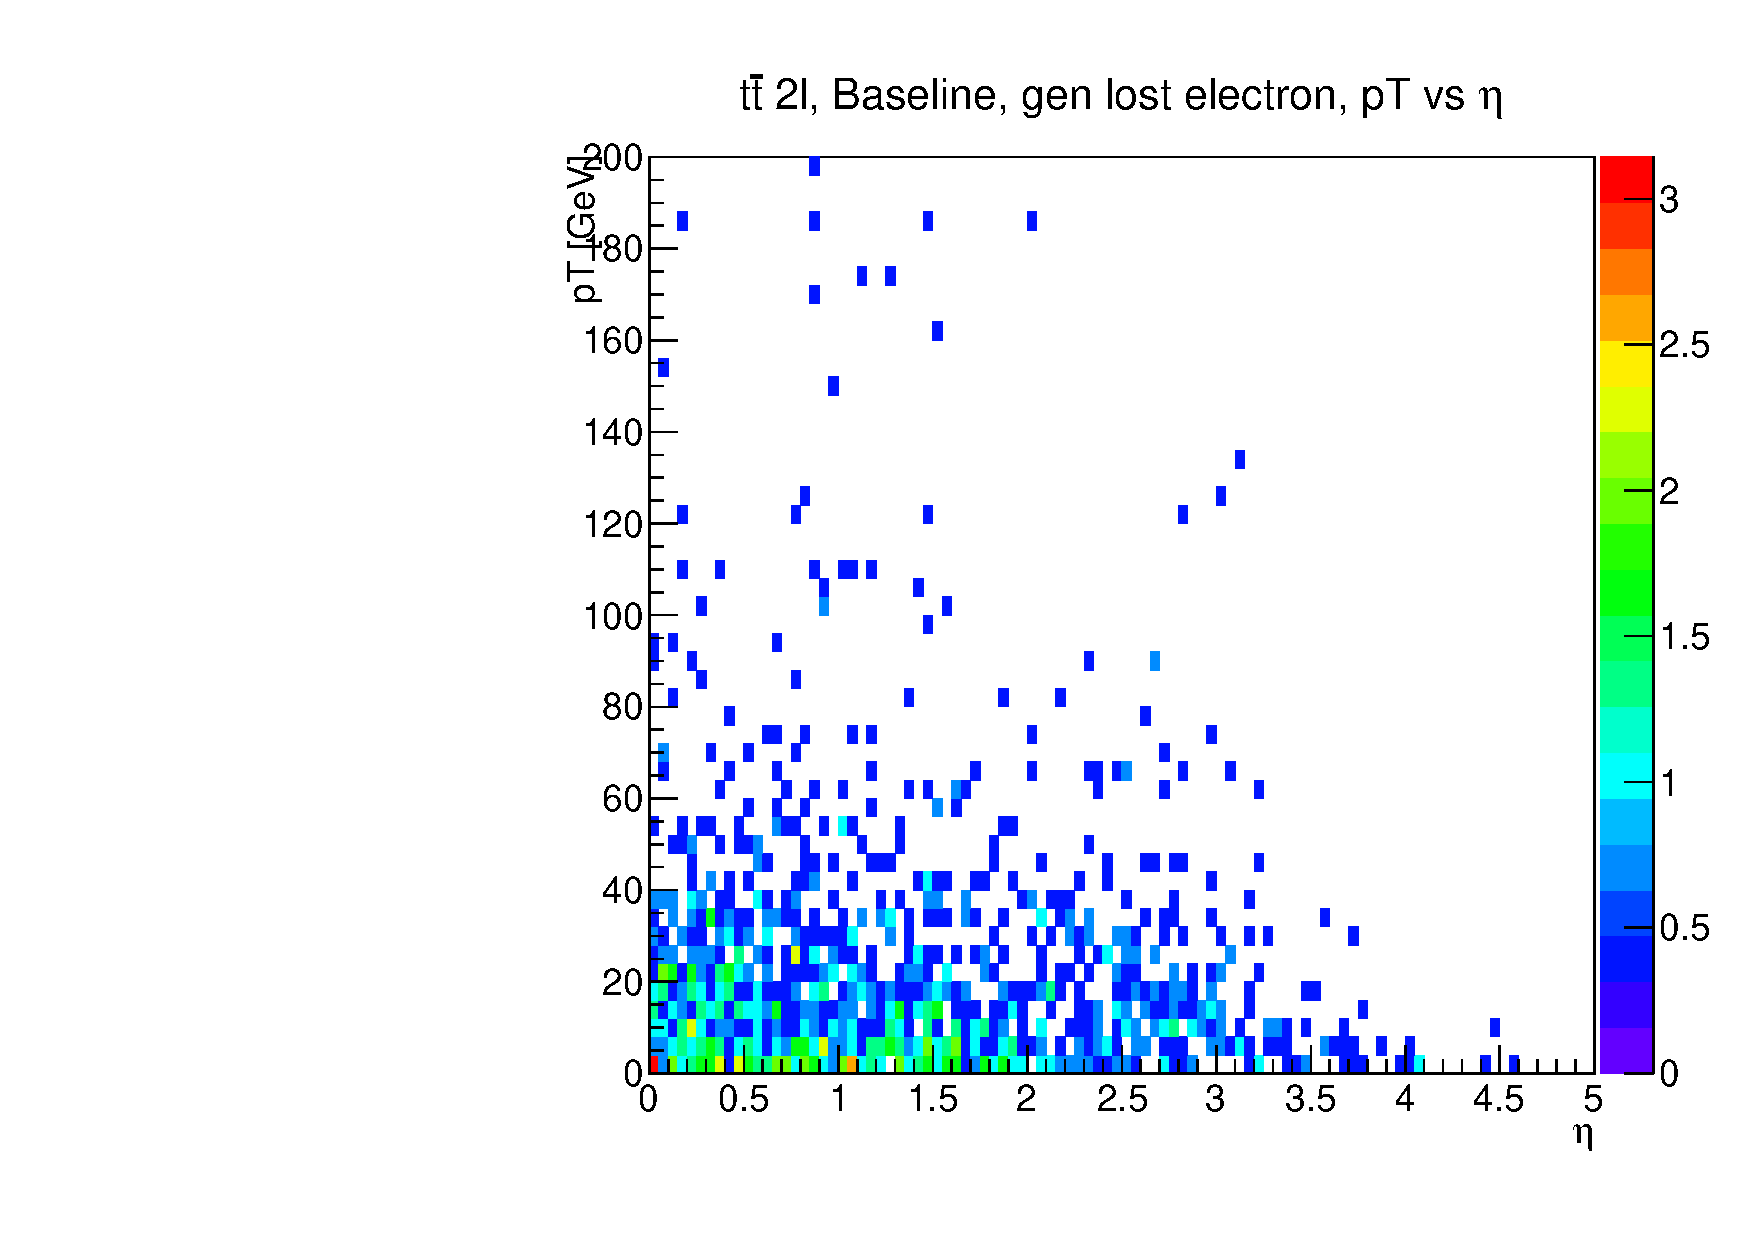
\includegraphics[width=0.32\textwidth]{Figures/studiesLostLepton/lostLeptonStudies__ttbar2l__genLostElectron__pt_vs_eta.pdf}
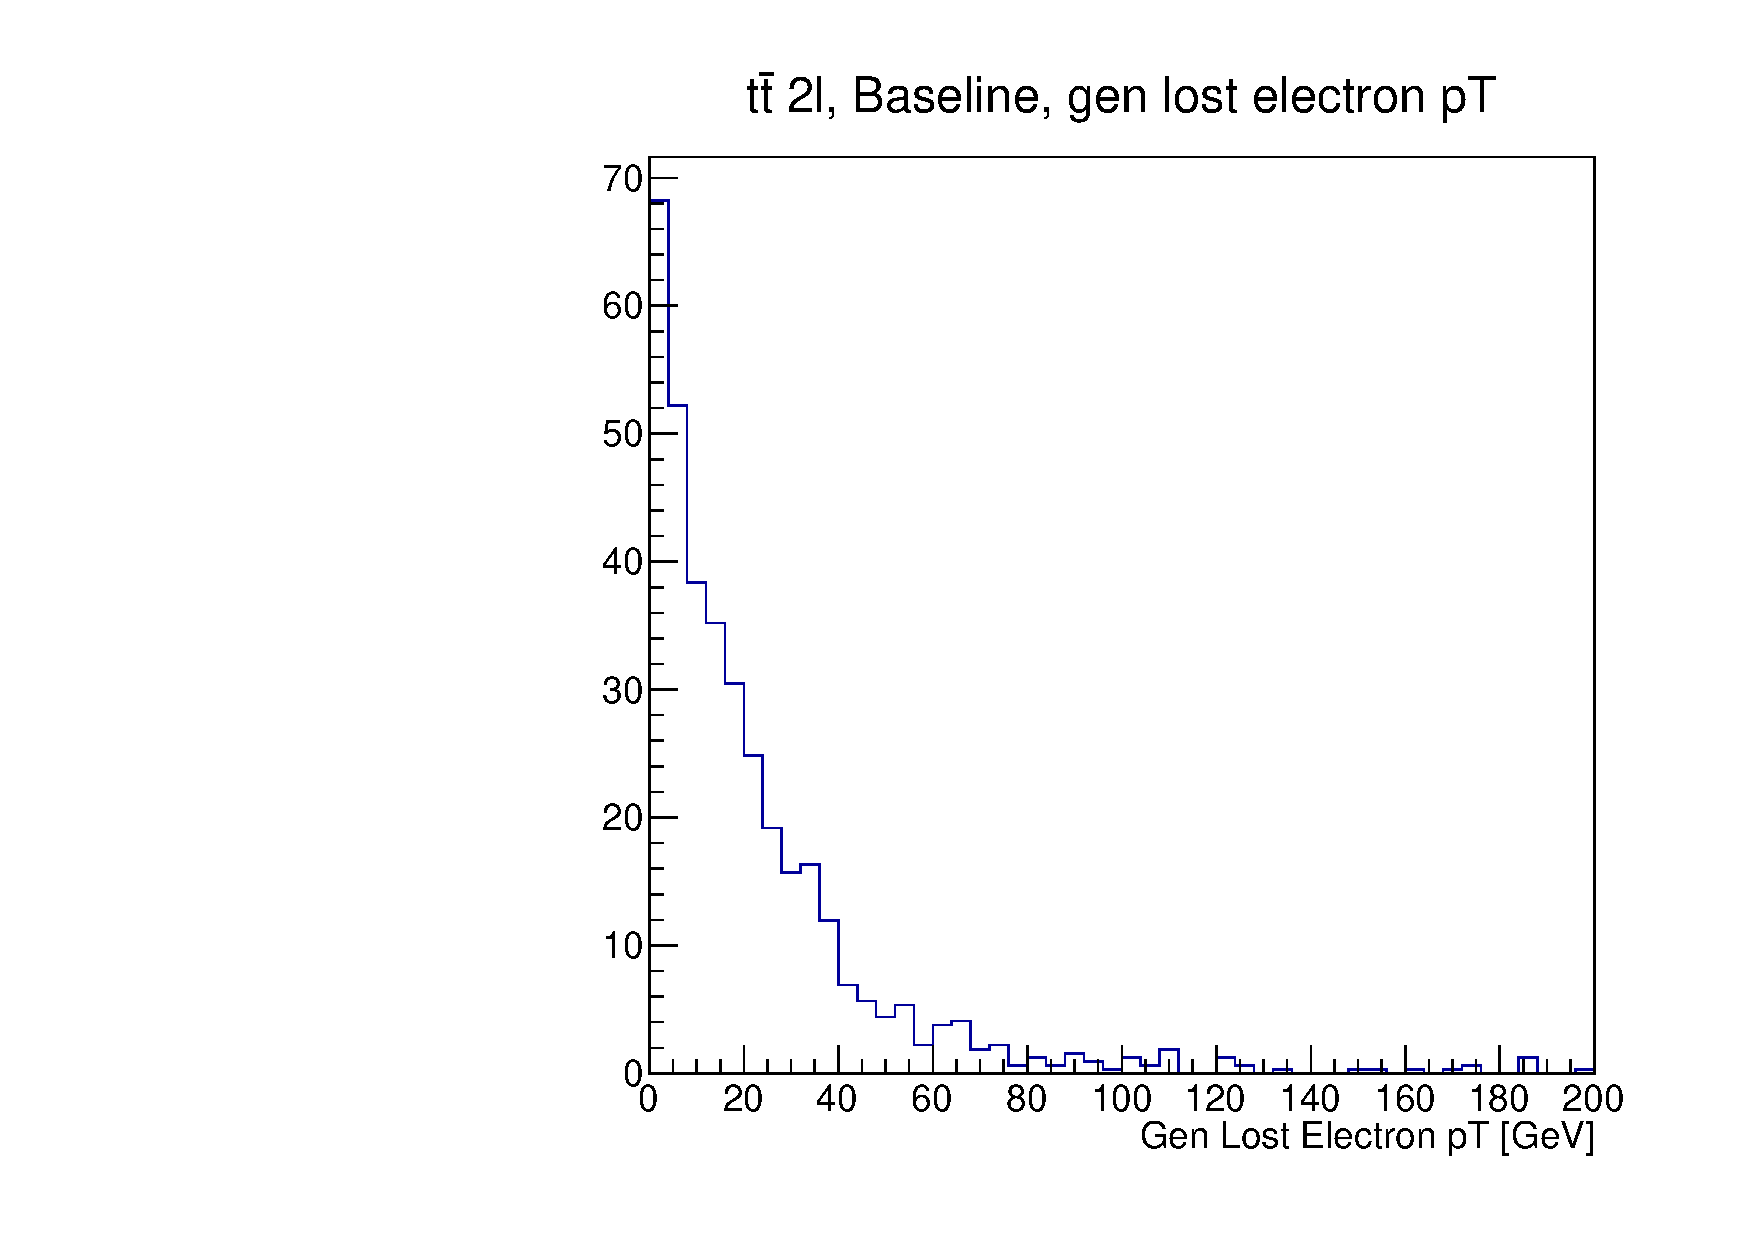
\includegraphics[width=0.32\textwidth]{Figures/studiesLostLepton/lostLeptonStudies__ttbar2l__genLostElectron__pt_vs_eta__projectionY__pt.pdf}
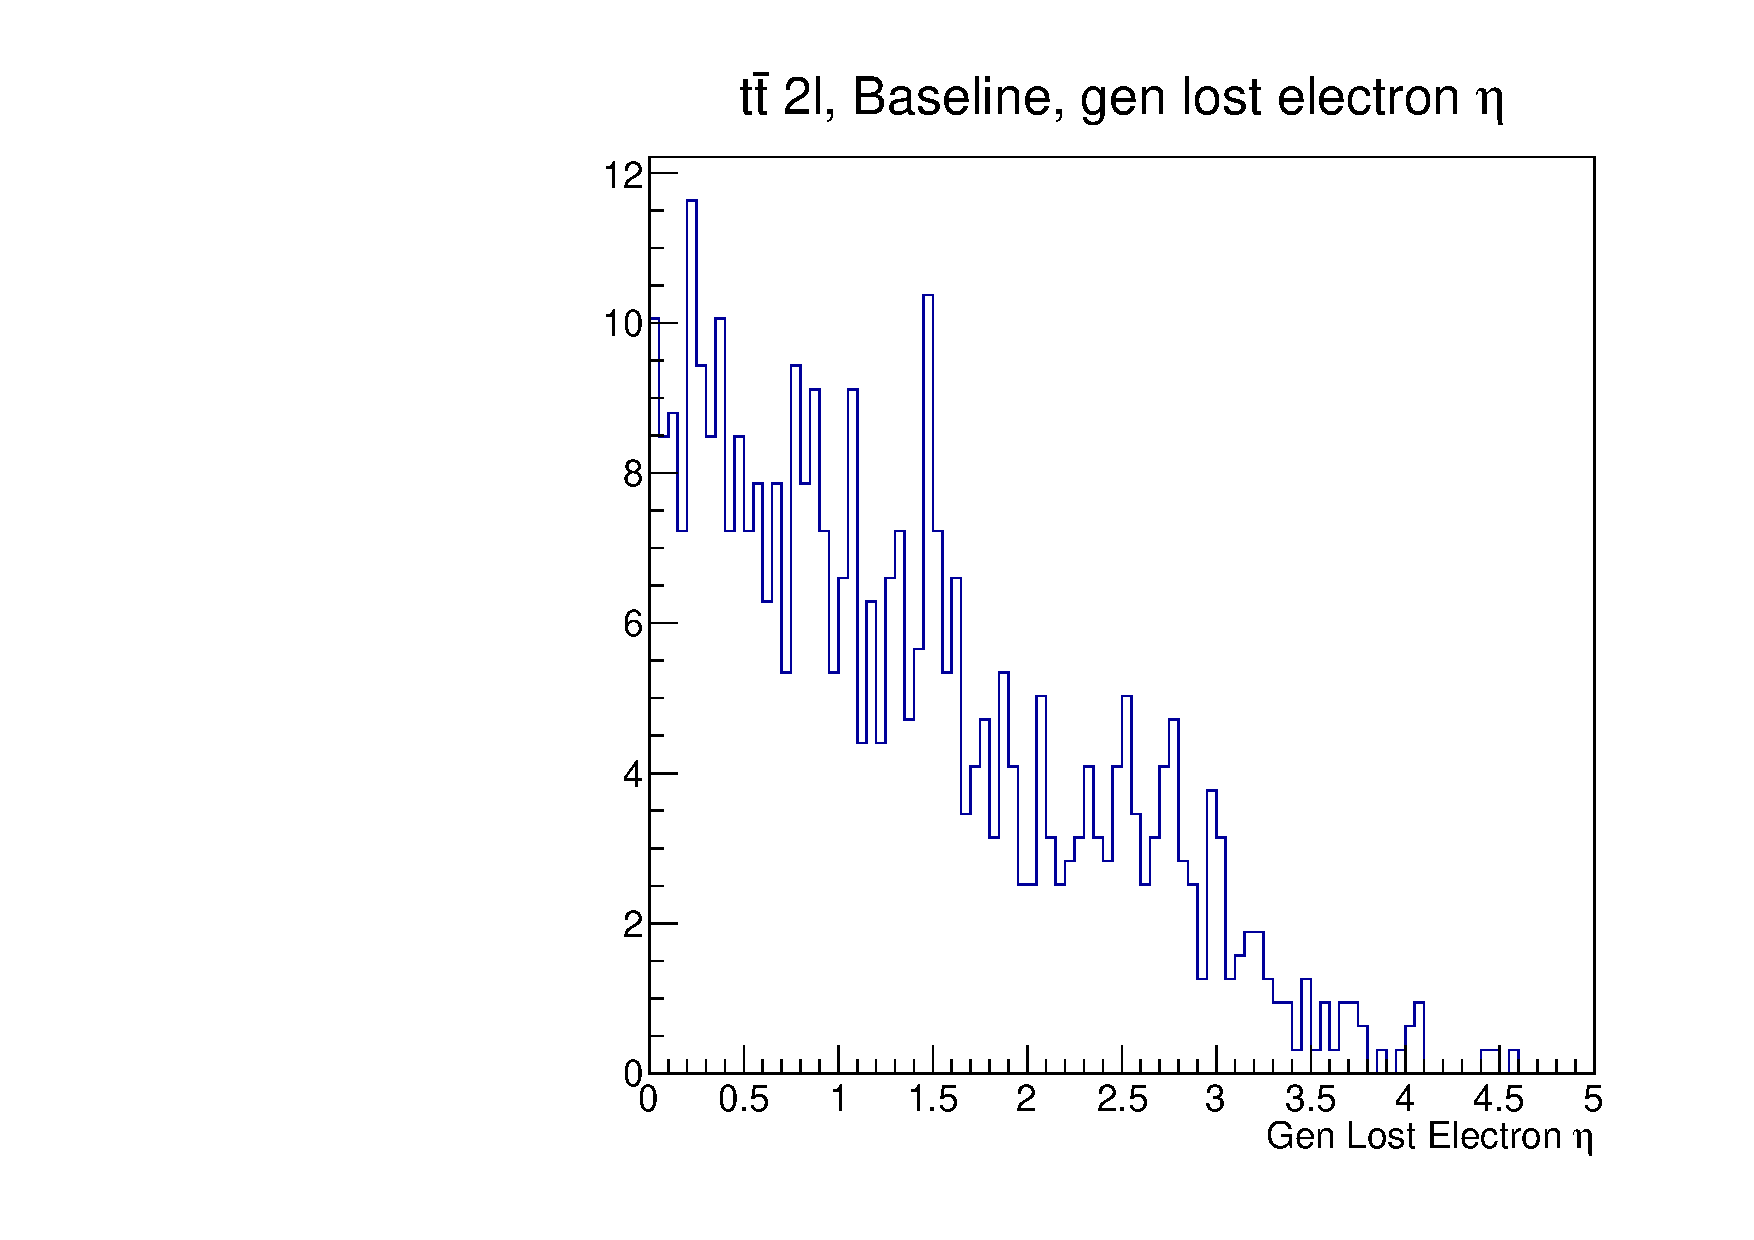
\includegraphics[width=0.32\textwidth]{Figures/studiesLostLepton/lostLeptonStudies__ttbar2l__genLostElectron__pt_vs_eta__projectionX__eta.pdf}
\caption{\label{fig:lost_lepton_studies:el_acceptance} (Left) Lost gen electron $p_{T}$ vs $\eta$, (Center) Projection from left-most plot, lost gen electron $p_{T}$ distribution, (Right) Projeciton from left-most plot, lost gen electron $\eta$ distribution.  Overall, only approximately 57\% of gen lost electrons pass acceptance }
\end{figure}

For muons, there are similar distributions in $p_{t}$ and $\eta$, for the lost gen muon.  While most events fail the $p_{T}>5$GeV cut, there are relatively more events, compared to gen lost electrons, that fail the $\eta<2.4$ acceptance cut.  


\subsection{Optimization of 8 TeV Lost Lepton Vetos for 13 TeV}
\label{sec:lost_lepton_studies:optimization}



\subsection{Details of Lost Lepton Background Estimate}
\label{sec:bkgLL_details}

This appendix discusses details of the lost lepton background estimate.  The subsection \ref{sec:bkgLL_details:tables} describes the effects of each systematic uncertainty considered on each of the components of the calculation.

\subsubsection{Uncertainty tables}
\label{sec:bkgLL_details:tables}

The uncertainties are described as follows:
\begin{itemize}
  \item Data and MC statisitics - the largest uncertainty is comes from the statistical error from the observered data
  \item bTagging Heavy Flavour, SF - the variation of the heavy flavour component of the bTagging reweighting, as provided by the BTV pog.
  \item bTagging Light Flavour, SF - the variation of the light flavour component of hte bTagging reweightingm as provided by the BTV pog.
  \item lepton SF - the varation of the lepton scale factors, as provided by the SUSY group.  Scale factors for both ID and isolation are applied.
  \item top pT  - although the reweighting is not applied as a scale factor, an additional uncertainty is taken to account for the difference in yields if the reweighting is applied. 
  \item nJets K3, K4 - these are the varations, from statistical errors from the nJets scale factors applied to ttbar->2l, as described in the previous section. 
  \item PDF - the method used is to take the average of 100 different PDF variations, and use the standard deviation of this average to vary the acceptance on the MC
  \item $\alpha_{S}$ - this method varies the QCD scale of the event to change the acceptance. 
  \item $Q^{2}$ - the largest two variations in renormalization and factorization scale are taken as an envelope.  
  \item JES - the jet energy scale is varied, to account for diffences in jet acceptance.  
\end{itemize}


\begin{table}
\begin{center}
\small
\caption{\label{tab:ll_estimate_sysUnc_lowDM_met_250_325} Table of uncertainties for the diLepton background estimate in the low deltaM signal region, $\ge$4 jets, and $250<\MET<325$ }
\scalebox{0.6}{
\begin{tabular}{|l|c|c|c|c|c|c|c|} \hline 
Systematic & $N_{Incl}^{CR},~(\%)$ & $M_{2\ell}^{SR},~(\%)$ & $M_{Incl}^{CR},~(\%)$ & $M_{2\ell}^{SR}/M_{Incl}^{CR},~(\%)$ & $M_{MET,nJet~bin}^{SR},~(\%)$ & $M_{MET,nJet~bin}^{SR}/M_{2\ell}^{SR},~(\%)$ & $N_{2\ell,estimate}^{SR},~(\%)$ \\ \hline 
Nominal & 66.00 & 40.67 & 67.00 & 0.61 & 18.66 & 0.46 & 18.39 \\ \hline \hline 
Data Stats Up & 74.12 ~(12.31\%) & 40.67 ~(0.00\%) & 67.00 ~(0.00\%) & 0.61 ~(0.00\%) & 18.66 ~(0.00\%) & 0.46 ~(0.00\%) & 20.65 ~(12.31\%) \\  
Data Stats Down & 57.88 ~(-12.31\%) & 40.67 ~(0.00\%) & 67.00 ~(0.00\%) & 0.61 ~(0.00\%) & 18.66 ~(0.00\%) & 0.46 ~(0.00\%) & 16.12 ~(-12.31\%) \\ \hline 
MC Stats Up & 66.00 ~(0.00\%) & 41.57 ~(2.22\%) & 68.14 ~(1.70\%) & 0.62 ~(1.70\%) & 19.26 ~(3.17\%) & 0.47 ~(2.07\%) & 18.88 ~(2.68\%) \\  
MC Stats Down & 66.00 ~(0.00\%) & 39.76 ~(-2.22\%) & 65.86 ~(-1.70\%) & 0.60 ~(-1.70\%) & 18.07 ~(-3.17\%) & 0.45 ~(-2.07\%) & 17.89 ~(-2.68\%) \\ \hline 
$Luminosity,~Up$ & 66.00,~(0.00\%) & 42.54,~(4.60\%) & 70.08~(4.60\%) & 0.61 ~(0.00\%) & 19.52 ~(4.60\%) & 0.46 ~(0.00\%) & 18.39 ~(0.00\%) \\  
$Luminosity,~Down$ & 66.00,~(0.00\%) & 38.80,~(-4.60\%) & 63.92~(-4.60\%) & 0.61 ~(0.00\%) & 17.81 ~(-4.60\%) & 0.46 ~(0.00\%) & 18.39 ~(0.00\%) \\ \hline 
$bTag~Efficiency,~Heavy~Flavour,~Up$ & 66.00,~(0.00\%) & 41.53,~(2.12\%) & 68.61~(2.41\%) & 0.61 ~(-0.28\%) & 19.08 ~(2.21\%) & 0.46 ~(0.08\%) & 18.35 ~(-0.20\%) \\  
$bTag~Efficiency,~Heavy~Flavour,~Down$ & 66.00,~(0.00\%) & 39.80,~(-2.12\%) & 65.38~(-2.41\%) & 0.61 ~(0.30\%) & 18.25 ~(-2.21\%) & 0.46 ~(-0.09\%) & 18.42 ~(0.21\%) \\ \hline 
$bTag~Efficiency,~Light~Flavour,~Up$ & 66.00,~(0.00\%) & 40.81,~(0.34\%) & 68.61~(2.41\%) & 0.59 ~(-2.02\%) & 18.75 ~(0.45\%) & 0.46 ~(0.10\%) & 18.03 ~(-1.91\%) \\  
$bTag~Efficiency,~Light~Flavour,~Down$ & 66.00,~(0.00\%) & 40.53,~(-0.34\%) & 65.38~(-2.41\%) & 0.62 ~(2.12\%) & 18.58 ~(-0.45\%) & 0.46 ~(-0.11\%) & 18.76 ~(2.01\%) \\ \hline 
$lepton~SF,~Up$ & 66.00,~(0.00\%) & 39.99,~(-1.67\%) & 67.09~(0.13\%) & 0.60 ~(-1.80\%) & 18.33 ~(-1.79\%) & 0.46 ~(-0.13\%) & 18.03 ~(-1.92\%) \\  
$lepton~SF,~Down$ & 66.00,~(0.00\%) & 41.34,~(1.65\%) & 65.53~(-2.19\%) & 0.63 ~(3.93\%) & 19.00 ~(1.77\%) & 0.46 ~(0.12\%) & 19.13 ~(4.05\%) \\ \hline 
$top~p_{T}~SF,~Up$ & 66.00,~(0.00\%) & 32.51,~(-20.06\%) & 52.11~(-22.22\%) & 0.62 ~(2.78\%) & 15.33 ~(-17.87\%) & 0.47 ~(2.73\%) & 19.41 ~(5.59\%) \\  
$top~p_{T}~SF,~Down$ & 66.00,~(0.00\%) & 40.67,~(0.00\%) & 67.00~(0.00\%) & 0.61 ~(0.00\%) & 18.66 ~(0.00\%) & 0.46 ~(0.00\%) & 18.39 ~(0.00\%) \\ \hline 
$nJets~SF,~K3,~K4,~Up$ & 66.00,~(0.00\%) & 42.97,~(5.65\%) & 70.75~(5.59\%) & 0.61 ~(0.06\%) & 19.78 ~(5.97\%) & 0.46 ~(0.30\%) & 18.45 ~(0.36\%) \\  
$nJets~SF,~K3,~K4,~Down$ & 66.00,~(0.00\%) & 38.37,~(-5.65\%) & 63.25~(-5.59\%) & 0.61 ~(-0.07\%) & 17.55 ~(-5.97\%) & 0.46 ~(-0.34\%) & 18.31 ~(-0.40\%) \\ \hline 
$PDF,~Up$ & 66.00,~(0.00\%) & 41.50,~(2.05\%) & 68.26~(1.88\%) & 0.61 ~(0.16\%) & 19.04 ~(1.99\%) & 0.46 ~(-0.06\%) & 18.41 ~(0.11\%) \\  
$PDF,~Down$ & 66.00,~(0.00\%) & 39.83,~(-2.05\%) & 65.74~(-1.88\%) & 0.61 ~(-0.17\%) & 18.29 ~(-1.99\%) & 0.46 ~(0.06\%) & 18.37 ~(-0.11\%) \\ \hline 
$\alpha_{S},~Up$ & 66.00,~(0.00\%) & 40.03,~(-1.57\%) & 65.96~(-1.55\%) & 0.61 ~(-0.02\%) & 18.37 ~(-1.57\%) & 0.46 ~(0.00\%) & 18.38 ~(-0.01\%) \\  
$\alpha_{S},~Down$ & 66.00,~(0.00\%) & 41.22,~(1.36\%) & 67.81~(1.22\%) & 0.61 ~(0.14\%) & 18.92 ~(1.37\%) & 0.46 ~(0.01\%) & 18.41 ~(0.15\%) \\ \hline 
$Q^{2},~Up$ & 66.00,~(0.00\%) & 32.77,~(-19.42\%) & 54.13~(-19.21\%) & 0.61 ~(-0.26\%) & 14.99 ~(-19.67\%) & 0.46 ~(-0.31\%) & 18.28 ~(-0.56\%) \\  
$Q^{2},~Down$ & 66.00,~(0.00\%) & 51.86,~(27.52\%) & 85.14~(27.08\%) & 0.61 ~(0.35\%) & 23.89 ~(28.02\%) & 0.46 ~(0.39\%) & 18.52 ~(0.74\%) \\ \hline 
JES Up & 66.00,~(0.00\%) & 43.10,~(5.97\%) & 70.79~(5.65\%) & 0.61 ~(0.31\%) & 19.94 ~(6.82\%) & 0.46 ~(0.80\%) & 18.59 ~(1.11\%) \\  
JES Down & 66.00,~(0.00\%) & 37.35,~(-8.14\%) & 61.80~(-7.77\%) & 0.60 ~(-0.41\%) & 16.96 ~(-9.13\%) & 0.45 ~(-1.07\%) & 18.11 ~(-1.48\%) \\ \hline \hline 
Total Uncertainties & 12.31\% & & & 5.56\% & & 3.64\% & 14.61\% \\ \hline 
\end{tabular} 
}
\end{center}
\end{table}


\begin{table}
\begin{center}
\small
\caption{\label{tab:ll_estimate_sysUnc_lowDM_met_325_inf} Table of uncertainties for the diLepton background estimate in the low deltaM signal region, $\ge$4 jets, and $\MET>325$ }
\scalebox{0.6}{
\begin{tabular}{|l|c|c|c|c|c|c|c|} \hline 
Systematic & $N_{Incl}^{CR},~(\%)$ & $M_{2\ell}^{SR},~(\%)$ & $M_{Incl}^{CR},~(\%)$ & $M_{2\ell}^{SR}/M_{Incl}^{CR},~(\%)$ & $M_{MET,nJet~bin}^{SR},~(\%)$ & $M_{MET,nJet~bin}^{SR}/M_{2\ell}^{SR},~(\%)$ & $N_{2\ell,estimate}^{SR},~(\%)$ \\ \hline 
Nominal & 66.00 & 40.67 & 67.00 & 0.61 & 8.21 & 0.20 & 8.09 \\ \hline \hline 
Data Stats Up & 74.12 ~(12.31\%) & 40.67 ~(0.00\%) & 67.00 ~(0.00\%) & 0.61 ~(0.00\%) & 8.21 ~(0.00\%) & 0.20 ~(0.00\%) & 9.08 ~(12.31\%) \\  
Data Stats Down & 57.88 ~(-12.31\%) & 40.67 ~(0.00\%) & 67.00 ~(0.00\%) & 0.61 ~(0.00\%) & 8.21 ~(0.00\%) & 0.20 ~(0.00\%) & 7.09 ~(-12.31\%) \\ \hline 
MC Stats Up & 66.00 ~(0.00\%) & 41.57 ~(2.22\%) & 68.14 ~(1.70\%) & 0.62 ~(1.70\%) & 8.62 ~(4.97\%) & 0.21 ~(3.80\%) & 8.43 ~(4.16\%) \\  
MC Stats Down & 66.00 ~(0.00\%) & 39.76 ~(-2.22\%) & 65.86 ~(-1.70\%) & 0.60 ~(-1.70\%) & 7.80 ~(-4.97\%) & 0.19 ~(-3.80\%) & 7.75 ~(-4.16\%) \\ \hline 
$Luminosity,~Up$ & 66.00,~(0.00\%) & 42.54,~(4.60\%) & 70.08~(4.60\%) & 0.61 ~(0.00\%) & 8.59 ~(4.60\%) & 0.20 ~(-0.00\%) & 8.09 ~(-0.00\%) \\  
$Luminosity,~Down$ & 66.00,~(0.00\%) & 38.80,~(-4.60\%) & 63.92~(-4.60\%) & 0.61 ~(0.00\%) & 7.83 ~(-4.60\%) & 0.20 ~(0.00\%) & 8.09 ~(0.00\%) \\ \hline 
$bTag~Efficiency,~Heavy~Flavour,~Up$ & 66.00,~(0.00\%) & 41.53,~(2.12\%) & 68.61~(2.41\%) & 0.61 ~(-0.28\%) & 8.35 ~(1.71\%) & 0.20 ~(-0.41\%) & 8.03 ~(-0.69\%) \\  
$bTag~Efficiency,~Heavy~Flavour,~Down$ & 66.00,~(0.00\%) & 39.80,~(-2.12\%) & 65.38~(-2.41\%) & 0.61 ~(0.30\%) & 8.07 ~(-1.71\%) & 0.20 ~(0.43\%) & 8.15 ~(0.72\%) \\ \hline 
$bTag~Efficiency,~Light~Flavour,~Up$ & 66.00,~(0.00\%) & 40.81,~(0.34\%) & 68.61~(2.41\%) & 0.59 ~(-2.02\%) & 8.24 ~(0.38\%) & 0.20 ~(0.03\%) & 7.93 ~(-1.99\%) \\  
$bTag~Efficiency,~Light~Flavour,~Down$ & 66.00,~(0.00\%) & 40.53,~(-0.34\%) & 65.38~(-2.41\%) & 0.62 ~(2.12\%) & 8.18 ~(-0.38\%) & 0.20 ~(-0.03\%) & 8.26 ~(2.08\%) \\ \hline 
$lepton~SF,~Up$ & 66.00,~(0.00\%) & 39.99,~(-1.67\%) & 67.09~(0.13\%) & 0.60 ~(-1.80\%) & 8.06 ~(-1.83\%) & 0.20 ~(-0.16\%) & 7.93 ~(-1.95\%) \\  
$lepton~SF,~Down$ & 66.00,~(0.00\%) & 41.34,~(1.65\%) & 65.53~(-2.19\%) & 0.63 ~(3.93\%) & 8.36 ~(1.80\%) & 0.20 ~(0.15\%) & 8.42 ~(4.08\%) \\ \hline 
$top~p_{T}~SF,~Up$ & 66.00,~(0.00\%) & 32.51,~(-20.06\%) & 52.11~(-22.22\%) & 0.62 ~(2.78\%) & 6.00 ~(-26.87\%) & 0.18 ~(-8.53\%) & 7.60 ~(-5.99\%) \\  
$top~p_{T}~SF,~Down$ & 66.00,~(0.00\%) & 40.67,~(0.00\%) & 67.00~(0.00\%) & 0.61 ~(0.00\%) & 8.21 ~(0.00\%) & 0.20 ~(0.00\%) & 8.09 ~(0.00\%) \\ \hline 
$nJets~SF,~K3,~K4,~Up$ & 66.00,~(0.00\%) & 42.97,~(5.65\%) & 70.75~(5.59\%) & 0.61 ~(0.06\%) & 8.69 ~(5.80\%) & 0.20 ~(0.14\%) & 8.11 ~(0.20\%) \\  
$nJets~SF,~K3,~K4,~Down$ & 66.00,~(0.00\%) & 38.37,~(-5.65\%) & 63.25~(-5.59\%) & 0.61 ~(-0.07\%) & 7.74 ~(-5.80\%) & 0.20 ~(-0.16\%) & 8.07 ~(-0.22\%) \\ \hline 
$PDF,~Up$ & 66.00,~(0.00\%) & 41.50,~(2.05\%) & 68.26~(1.88\%) & 0.61 ~(0.16\%) & 8.44 ~(2.77\%) & 0.20 ~(0.71\%) & 8.16 ~(0.87\%) \\  
$PDF,~Down$ & 66.00,~(0.00\%) & 39.83,~(-2.05\%) & 65.74~(-1.88\%) & 0.61 ~(-0.17\%) & 7.98 ~(-2.77\%) & 0.20 ~(-0.73\%) & 8.02 ~(-0.90\%) \\ \hline 
$\alpha_{S},~Up$ & 66.00,~(0.00\%) & 40.03,~(-1.57\%) & 65.96~(-1.55\%) & 0.61 ~(-0.02\%) & 8.06 ~(-1.80\%) & 0.20 ~(-0.24\%) & 8.07 ~(-0.25\%) \\  
$\alpha_{S},~Down$ & 66.00,~(0.00\%) & 41.22,~(1.36\%) & 67.81~(1.22\%) & 0.61 ~(0.14\%) & 8.35 ~(1.66\%) & 0.20 ~(0.30\%) & 8.12 ~(0.44\%) \\ \hline 
$Q^{2},~Up$ & 66.00,~(0.00\%) & 32.77,~(-19.42\%) & 54.13~(-19.21\%) & 0.61 ~(-0.26\%) & 6.31 ~(-23.19\%) & 0.19 ~(-4.68\%) & 7.69 ~(-4.92\%) \\  
$Q^{2},~Down$ & 66.00,~(0.00\%) & 51.86,~(27.52\%) & 85.14~(27.08\%) & 0.61 ~(0.35\%) & 11.11 ~(35.26\%) & 0.21 ~(6.07\%) & 8.61 ~(6.44\%) \\ \hline 
JES Up & 66.00,~(0.00\%) & 43.10,~(5.97\%) & 70.79~(5.65\%) & 0.61 ~(0.31\%) & 8.60 ~(4.68\%) & 0.20 ~(-1.22\%) & 8.01 ~(-0.92\%) \\  
JES Down & 66.00,~(0.00\%) & 37.35,~(-8.14\%) & 61.80~(-7.77\%) & 0.60 ~(-0.41\%) & 7.73 ~(-5.90\%) & 0.21 ~(2.44\%) & 8.25 ~(2.02\%) \\ \hline \hline 
Total Uncertainties & 12.31\% & & & 5.56\% & & 11.44\% & 16.52\% \\ \hline 
\end{tabular} 
}
\end{center}
\end{table}


\begin{table}
\begin{center}
\small
\caption{\label{tab:ll_estimate_sysUnc_highDM_met_250_350} Table of uncertainties for the diLepton background estimate in the high deltaM signal region, $\ge$4 jets, and $250<\MET<350$ }
\scalebox{0.6}{
\begin{tabular}{|l|c|c|c|c|c|c|c|} \hline 
Systematic & $N_{Incl}^{CR},~(\%)$ & $M_{2\ell}^{SR},~(\%)$ & $M_{Incl}^{CR},~(\%)$ & $M_{2\ell}^{SR}/M_{Incl}^{CR},~(\%)$ & $M_{MET,nJet~bin}^{SR},~(\%)$ & $M_{MET,nJet~bin}^{SR}/M_{2\ell}^{SR},~(\%)$ & $N_{2\ell,estimate}^{SR},~(\%)$ \\ \hline 
Nominal & 18.00 & 11.19 & 25.55 & 0.44 & 4.17 & 0.37 & 2.94 \\ \hline \hline 
Data Stats Up & 22.24 ~(23.57\%) & 11.19 ~(0.00\%) & 25.55 ~(0.00\%) & 0.44 ~(0.00\%) & 4.17 ~(0.00\%) & 0.37 ~(0.00\%) & 3.63 ~(23.57\%) \\  
Data Stats Down & 13.76 ~(-23.57\%) & 11.19 ~(0.00\%) & 25.55 ~(0.00\%) & 0.44 ~(0.00\%) & 4.17 ~(0.00\%) & 0.37 ~(0.00\%) & 2.24 ~(-23.57\%) \\ \hline 
MC Stats Up & 18.00 ~(0.00\%) & 11.75 ~(5.01\%) & 26.44 ~(3.49\%) & 0.45 ~(3.49\%) & 4.49 ~(7.80\%) & 0.39 ~(4.46\%) & 3.10 ~(5.66\%) \\  
MC Stats Down & 18.00 ~(0.00\%) & 10.63 ~(-5.01\%) & 24.66 ~(-3.49\%) & 0.42 ~(-3.49\%) & 3.84 ~(-7.80\%) & 0.36 ~(-4.46\%) & 2.77 ~(-5.66\%) \\ \hline 
$Luminosity,~Up$ & 18.00,~(0.00\%) & 11.71,~(4.60\%) & 26.72~(4.60\%) & 0.44 ~(0.00\%) & 4.36 ~(4.60\%) & 0.37 ~(-0.00\%) & 2.94 ~(-0.00\%) \\  
$Luminosity,~Down$ & 18.00,~(0.00\%) & 10.68,~(-4.60\%) & 24.37~(-4.60\%) & 0.44 ~(0.00\%) & 3.97 ~(-4.60\%) & 0.37 ~(-0.00\%) & 2.94 ~(0.00\%) \\ \hline 
$bTag~Efficiency,~Heavy~Flavour,~Up$ & 18.00,~(0.00\%) & 11.55,~(3.16\%) & 26.29~(2.92\%) & 0.44 ~(0.24\%) & 4.30 ~(3.11\%) & 0.37 ~(-0.04\%) & 2.94 ~(0.19\%) \\  
$bTag~Efficiency,~Heavy~Flavour,~Down$ & 18.00,~(0.00\%) & 10.84,~(-3.16\%) & 24.80~(-2.92\%) & 0.44 ~(-0.25\%) & 4.04 ~(-3.11\%) & 0.37 ~(0.05\%) & 2.93 ~(-0.20\%) \\ \hline 
$bTag~Efficiency,~Light~Flavour,~Up$ & 18.00,~(0.00\%) & 11.36,~(1.52\%) & 26.29~(2.92\%) & 0.43 ~(-1.36\%) & 4.25 ~(2.00\%) & 0.37 ~(0.48\%) & 2.91 ~(-0.89\%) \\  
$bTag~Efficiency,~Light~Flavour,~Down$ & 18.00,~(0.00\%) & 11.02,~(-1.52\%) & 24.80~(-2.92\%) & 0.44 ~(1.44\%) & 4.08 ~(-2.00\%) & 0.37 ~(-0.49\%) & 2.96 ~(0.94\%) \\ \hline 
$lepton~SF,~Up$ & 18.00,~(0.00\%) & 10.95,~(-2.12\%) & 25.57~(0.07\%) & 0.43 ~(-2.19\%) & 4.07 ~(-2.21\%) & 0.37 ~(-0.08\%) & 2.87 ~(-2.28\%) \\  
$lepton~SF,~Down$ & 18.00,~(0.00\%) & 11.43,~(2.11\%) & 25.00~(-2.15\%) & 0.46 ~(4.35\%) & 4.26 ~(2.19\%) & 0.37 ~(0.08\%) & 3.07 ~(4.43\%) \\ \hline 
$top~p_{T}~SF,~Up$ & 18.00,~(0.00\%) & 9.29,~(-17.01\%) & 21.27~(-16.73\%) & 0.44 ~(-0.34\%) & 3.48 ~(-16.55\%) & 0.37 ~(0.56\%) & 2.94 ~(0.22\%) \\  
$top~p_{T}~SF,~Down$ & 18.00,~(0.00\%) & 11.19,~(0.00\%) & 25.55~(0.00\%) & 0.44 ~(0.00\%) & 4.17 ~(0.00\%) & 0.37 ~(0.00\%) & 2.94 ~(0.00\%) \\ \hline 
$nJets~SF,~K3,~K4,~Up$ & 18.00,~(0.00\%) & 11.69,~(4.48\%) & 26.54~(3.89\%) & 0.44 ~(0.56\%) & 4.37 ~(4.92\%) & 0.37 ~(0.42\%) & 2.96 ~(0.99\%) \\  
$nJets~SF,~K3,~K4,~Down$ & 18.00,~(0.00\%) & 10.69,~(-4.48\%) & 24.55~(-3.89\%) & 0.44 ~(-0.61\%) & 3.96 ~(-4.92\%) & 0.37 ~(-0.46\%) & 2.90 ~(-1.07\%) \\ \hline 
$PDF,~Up$ & 18.00,~(0.00\%) & 11.44,~(2.21\%) & 25.97~(1.66\%) & 0.44 ~(0.55\%) & 4.28 ~(2.61\%) & 0.37 ~(0.39\%) & 2.96 ~(0.94\%) \\  
$PDF,~Down$ & 18.00,~(0.00\%) & 10.94,~(-2.21\%) & 25.12~(-1.66\%) & 0.44 ~(-0.57\%) & 4.06 ~(-2.61\%) & 0.37 ~(-0.41\%) & 2.91 ~(-0.97\%) \\ \hline 
$\alpha_{S},~Up$ & 18.00,~(0.00\%) & 11.03,~(-1.41\%) & 25.24~(-1.19\%) & 0.44 ~(-0.21\%) & 4.10 ~(-1.52\%) & 0.37 ~(-0.12\%) & 2.93 ~(-0.33\%) \\  
$\alpha_{S},~Down$ & 18.00,~(0.00\%) & 11.35,~(1.38\%) & 25.79~(0.96\%) & 0.44 ~(0.42\%) & 4.23 ~(1.58\%) & 0.37 ~(0.19\%) & 2.95 ~(0.61\%) \\ \hline 
$Q^{2},~Up$ & 18.00,~(0.00\%) & 9.16,~(-18.11\%) & 21.68~(-15.13\%) & 0.42 ~(-3.50\%) & 3.38 ~(-18.76\%) & 0.37 ~(-0.80\%) & 2.81 ~(-4.28\%) \\  
$Q^{2},~Down$ & 18.00,~(0.00\%) & 14.14,~(26.31\%) & 31.00~(21.34\%) & 0.46 ~(4.10\%) & 5.30 ~(27.17\%) & 0.37 ~(0.68\%) & 3.08 ~(4.80\%) \\ \hline 
JES Up & 18.00,~(0.00\%) & 12.15,~(8.60\%) & 26.65~(4.30\%) & 0.46 ~(4.12\%) & 4.71 ~(12.97\%) & 0.39 ~(4.03\%) & 3.18 ~(8.32\%) \\  
JES Down & 18.00,~(0.00\%) & 10.52,~(-6.04\%) & 24.10~(-5.66\%) & 0.44 ~(-0.40\%) & 3.74 ~(-10.26\%) & 0.36 ~(-4.50\%) & 2.79 ~(-4.89\%) \\ \hline \hline 
Total Uncertainties & 23.57\% & & & 8.24\% & & 6.46\% & 26.51\% \\ \hline 
\end{tabular} 
}
\end{center}
\end{table}



\begin{table}
\begin{center}
\small
\caption{\label{tab:ll_estimate_sysUnc_highDM_met_350_450} Table of uncertainties for the diLepton background estimate in the high deltaM signal region, $\ge$4 jets, and $350<\MET<450$ }
\scalebox{0.6}{
\begin{tabular}{|l|c|c|c|c|c|c|c|} \hline 
Systematic & $N_{Incl}^{CR},~(\%)$ & $M_{2\ell}^{SR},~(\%)$ & $M_{Incl}^{CR},~(\%)$ & $M_{2\ell}^{SR}/M_{Incl}^{CR},~(\%)$ & $M_{MET,nJet~bin}^{SR},~(\%)$ & $M_{MET,nJet~bin}^{SR}/M_{2\ell}^{SR},~(\%)$ & $N_{2\ell,estimate}^{SR},~(\%)$ \\ \hline 
Nominal & 18.00 & 11.19 & 25.55 & 0.44 & 1.30 & 0.12 & 0.91 \\ \hline \hline 
Data Stats Up & 22.24 ~(23.57\%) & 11.19 ~(0.00\%) & 25.55 ~(0.00\%) & 0.44 ~(0.00\%) & 1.30 ~(0.00\%) & 0.12 ~(0.00\%) & 1.13 ~(23.57\%) \\  
Data Stats Down & 13.76 ~(-23.57\%) & 11.19 ~(0.00\%) & 25.55 ~(0.00\%) & 0.44 ~(0.00\%) & 1.30 ~(0.00\%) & 0.12 ~(0.00\%) & 0.70 ~(-23.57\%) \\ \hline 
MC Stats Up & 18.00 ~(0.00\%) & 11.75 ~(5.01\%) & 26.44 ~(3.49\%) & 0.45 ~(3.49\%) & 1.49 ~(14.85\%) & 0.13 ~(9.49\%) & 1.01 ~(10.11\%) \\  
MC Stats Down & 18.00 ~(0.00\%) & 10.63 ~(-5.01\%) & 24.66 ~(-3.49\%) & 0.42 ~(-3.49\%) & 1.10 ~(-14.85\%) & 0.10 ~(-9.49\%) & 0.82 ~(-10.11\%) \\ \hline 
$Luminosity,~Up$ & 18.00,~(0.00\%) & 11.71,~(4.60\%) & 26.72~(4.60\%) & 0.44 ~(0.00\%) & 1.36 ~(4.60\%) & 0.12 ~(-0.00\%) & 0.91 ~(-0.00\%) \\  
$Luminosity,~Down$ & 18.00,~(0.00\%) & 10.68,~(-4.60\%) & 24.37~(-4.60\%) & 0.44 ~(0.00\%) & 1.24 ~(-4.60\%) & 0.12 ~(-0.00\%) & 0.91 ~(0.00\%) \\ \hline 
$bTag~Efficiency,~Heavy~Flavour,~Up$ & 18.00,~(0.00\%) & 11.55,~(3.16\%) & 26.29~(2.92\%) & 0.44 ~(0.24\%) & 1.33 ~(2.38\%) & 0.11 ~(-0.76\%) & 0.91 ~(-0.52\%) \\  
$bTag~Efficiency,~Heavy~Flavour,~Down$ & 18.00,~(0.00\%) & 10.84,~(-3.16\%) & 24.80~(-2.92\%) & 0.44 ~(-0.25\%) & 1.26 ~(-2.38\%) & 0.12 ~(0.81\%) & 0.92 ~(0.56\%) \\ \hline 
$bTag~Efficiency,~Light~Flavour,~Up$ & 18.00,~(0.00\%) & 11.36,~(1.52\%) & 26.29~(2.92\%) & 0.43 ~(-1.36\%) & 1.32 ~(1.74\%) & 0.12 ~(0.22\%) & 0.90 ~(-1.15\%) \\  
$bTag~Efficiency,~Light~Flavour,~Down$ & 18.00,~(0.00\%) & 11.02,~(-1.52\%) & 24.80~(-2.92\%) & 0.44 ~(1.44\%) & 1.27 ~(-1.74\%) & 0.12 ~(-0.22\%) & 0.92 ~(1.21\%) \\ \hline 
$lepton~SF,~Up$ & 18.00,~(0.00\%) & 10.95,~(-2.12\%) & 25.57~(0.07\%) & 0.43 ~(-2.19\%) & 1.27 ~(-2.18\%) & 0.12 ~(-0.06\%) & 0.89 ~(-2.25\%) \\  
$lepton~SF,~Down$ & 18.00,~(0.00\%) & 11.43,~(2.11\%) & 25.00~(-2.15\%) & 0.46 ~(4.35\%) & 1.32 ~(2.16\%) & 0.12 ~(0.05\%) & 0.95 ~(4.40\%) \\ \hline 
$top~p_{T}~SF,~Up$ & 18.00,~(0.00\%) & 9.29,~(-17.01\%) & 21.27~(-16.73\%) & 0.44 ~(-0.34\%) & 1.06 ~(-18.48\%) & 0.11 ~(-1.77\%) & 0.89 ~(-2.10\%) \\  
$top~p_{T}~SF,~Down$ & 18.00,~(0.00\%) & 11.19,~(0.00\%) & 25.55~(0.00\%) & 0.44 ~(0.00\%) & 1.30 ~(0.00\%) & 0.12 ~(0.00\%) & 0.91 ~(0.00\%) \\ \hline 
$nJets~SF,~K3,~K4,~Up$ & 18.00,~(0.00\%) & 11.69,~(4.48\%) & 26.54~(3.89\%) & 0.44 ~(0.56\%) & 1.35 ~(4.41\%) & 0.12 ~(-0.07\%) & 0.92 ~(0.49\%) \\  
$nJets~SF,~K3,~K4,~Down$ & 18.00,~(0.00\%) & 10.69,~(-4.48\%) & 24.55~(-3.89\%) & 0.44 ~(-0.61\%) & 1.24 ~(-4.41\%) & 0.12 ~(0.08\%) & 0.91 ~(-0.53\%) \\ \hline 
$PDF,~Up$ & 18.00,~(0.00\%) & 11.44,~(2.21\%) & 25.97~(1.66\%) & 0.44 ~(0.55\%) & 1.33 ~(2.82\%) & 0.12 ~(0.59\%) & 0.92 ~(1.14\%) \\  
$PDF,~Down$ & 18.00,~(0.00\%) & 10.94,~(-2.21\%) & 25.12~(-1.66\%) & 0.44 ~(-0.57\%) & 1.26 ~(-2.82\%) & 0.12 ~(-0.62\%) & 0.90 ~(-1.18\%) \\ \hline 
$\alpha_{S},~Up$ & 18.00,~(0.00\%) & 11.03,~(-1.41\%) & 25.24~(-1.19\%) & 0.44 ~(-0.21\%) & 1.28 ~(-1.43\%) & 0.12 ~(-0.03\%) & 0.91 ~(-0.24\%) \\  
$\alpha_{S},~Down$ & 18.00,~(0.00\%) & 11.35,~(1.38\%) & 25.79~(0.96\%) & 0.44 ~(0.42\%) & 1.32 ~(1.57\%) & 0.12 ~(0.18\%) & 0.92 ~(0.60\%) \\ \hline 
$Q^{2},~Up$ & 18.00,~(0.00\%) & 9.16,~(-18.11\%) & 21.68~(-15.13\%) & 0.42 ~(-3.50\%) & 1.04 ~(-19.69\%) & 0.11 ~(-1.93\%) & 0.86 ~(-5.37\%) \\  
$Q^{2},~Down$ & 18.00,~(0.00\%) & 14.14,~(26.31\%) & 31.00~(21.34\%) & 0.46 ~(4.10\%) & 1.68 ~(29.88\%) & 0.12 ~(2.82\%) & 0.98 ~(7.04\%) \\ \hline 
JES Up & 18.00,~(0.00\%) & 12.15,~(8.60\%) & 26.65~(4.30\%) & 0.46 ~(4.12\%) & 1.36 ~(5.11\%) & 0.11 ~(-3.21\%) & 0.92 ~(0.78\%) \\  
JES Down & 18.00,~(0.00\%) & 10.52,~(-6.04\%) & 24.10~(-5.66\%) & 0.44 ~(-0.40\%) & 1.27 ~(-1.77\%) & 0.12 ~(4.54\%) & 0.95 ~(4.12\%) \\ \hline \hline 
Total Uncertainties & 23.57\% & & & 8.24\% & & 11.09\% & 27.42\% \\ \hline 
\end{tabular} 
}
\end{center}
\end{table}


\begin{table}
\begin{center}
\small
\caption{\label{tab:ll_estimate_sysUnc_highDM_met_450_inf} Table of uncertainties for the diLepton background estimate in the high deltaM signal region, $\ge$4 jets, and $\MET>450$ }
\scalebox{0.6}{
\begin{tabular}{|l|c|c|c|c|c|c|c|} \hline 
Systematic & $N_{Incl}^{CR},~(\%)$ & $M_{2\ell}^{SR},~(\%)$ & $M_{Incl}^{CR},~(\%)$ & $M_{2\ell}^{SR}/M_{Incl}^{CR},~(\%)$ & $M_{MET,nJet~bin}^{SR},~(\%)$ & $M_{MET,nJet~bin}^{SR}/M_{2\ell}^{SR},~(\%)$ & $N_{2\ell,estimate}^{SR},~(\%)$ \\ \hline 
Nominal & 18.00 & 11.19 & 25.55 & 0.44 & 0.91 & 0.08 & 0.64 \\ \hline \hline 
Data Stats Up & 22.24 ~(23.57\%) & 11.19 ~(0.00\%) & 25.55 ~(0.00\%) & 0.44 ~(0.00\%) & 0.91 ~(0.00\%) & 0.08 ~(0.00\%) & 0.79 ~(23.57\%) \\  
Data Stats Down & 13.76 ~(-23.57\%) & 11.19 ~(0.00\%) & 25.55 ~(0.00\%) & 0.44 ~(0.00\%) & 0.91 ~(0.00\%) & 0.08 ~(0.00\%) & 0.49 ~(-23.57\%) \\ \hline 
MC Stats Up & 18.00 ~(0.00\%) & 11.75 ~(5.01\%) & 26.44 ~(3.49\%) & 0.45 ~(3.49\%) & 1.07 ~(17.92\%) & 0.09 ~(11.56\%) & 0.72 ~(12.07\%) \\  
MC Stats Down & 18.00 ~(0.00\%) & 10.63 ~(-5.01\%) & 24.66 ~(-3.49\%) & 0.42 ~(-3.49\%) & 0.74 ~(-17.92\%) & 0.07 ~(-11.56\%) & 0.56 ~(-12.07\%) \\ \hline 
$Luminosity,~Up$ & 18.00,~(0.00\%) & 11.71,~(4.60\%) & 26.72~(4.60\%) & 0.44 ~(0.00\%) & 0.95 ~(4.60\%) & 0.08 ~(-0.00\%) & 0.64 ~(-0.00\%) \\  
$Luminosity,~Down$ & 18.00,~(0.00\%) & 10.68,~(-4.60\%) & 24.37~(-4.60\%) & 0.44 ~(0.00\%) & 0.87 ~(-4.60\%) & 0.08 ~(-0.00\%) & 0.64 ~(0.00\%) \\ \hline 
$bTag~Efficiency,~Heavy~Flavour,~Up$ & 18.00,~(0.00\%) & 11.55,~(3.16\%) & 26.29~(2.92\%) & 0.44 ~(0.24\%) & 0.93 ~(2.11\%) & 0.08 ~(-1.02\%) & 0.63 ~(-0.78\%) \\  
$bTag~Efficiency,~Heavy~Flavour,~Down$ & 18.00,~(0.00\%) & 10.84,~(-3.16\%) & 24.80~(-2.92\%) & 0.44 ~(-0.25\%) & 0.89 ~(-2.11\%) & 0.08 ~(1.08\%) & 0.64 ~(0.83\%) \\ \hline 
$bTag~Efficiency,~Light~Flavour,~Up$ & 18.00,~(0.00\%) & 11.36,~(1.52\%) & 26.29~(2.92\%) & 0.43 ~(-1.36\%) & 0.92 ~(0.91\%) & 0.08 ~(-0.60\%) & 0.63 ~(-1.95\%) \\  
$bTag~Efficiency,~Light~Flavour,~Down$ & 18.00,~(0.00\%) & 11.02,~(-1.52\%) & 24.80~(-2.92\%) & 0.44 ~(1.44\%) & 0.90 ~(-0.91\%) & 0.08 ~(0.62\%) & 0.65 ~(2.07\%) \\ \hline 
$lepton~SF,~Up$ & 18.00,~(0.00\%) & 10.95,~(-2.12\%) & 25.57~(0.07\%) & 0.43 ~(-2.19\%) & 0.86 ~(-5.71\%) & 0.08 ~(-3.67\%) & 0.60 ~(-5.78\%) \\  
$lepton~SF,~Down$ & 18.00,~(0.00\%) & 11.43,~(2.11\%) & 25.00~(-2.15\%) & 0.46 ~(4.35\%) & 0.96 ~(5.67\%) & 0.08 ~(3.49\%) & 0.69 ~(7.99\%) \\ \hline 
$top~p_{T}~SF,~Up$ & 18.00,~(0.00\%) & 9.29,~(-17.01\%) & 21.27~(-16.73\%) & 0.44 ~(-0.34\%) & 0.65 ~(-28.17\%) & 0.07 ~(-13.45\%) & 0.55 ~(-13.74\%) \\  
$top~p_{T}~SF,~Down$ & 18.00,~(0.00\%) & 11.19,~(0.00\%) & 25.55~(0.00\%) & 0.44 ~(0.00\%) & 0.91 ~(0.00\%) & 0.08 ~(0.00\%) & 0.64 ~(0.00\%) \\ \hline 
$nJets~SF,~K3,~K4,~Up$ & 18.00,~(0.00\%) & 11.69,~(4.48\%) & 26.54~(3.89\%) & 0.44 ~(0.56\%) & 0.95 ~(4.61\%) & 0.08 ~(0.12\%) & 0.64 ~(0.69\%) \\  
$nJets~SF,~K3,~K4,~Down$ & 18.00,~(0.00\%) & 10.69,~(-4.48\%) & 24.55~(-3.89\%) & 0.44 ~(-0.61\%) & 0.87 ~(-4.61\%) & 0.08 ~(-0.13\%) & 0.63 ~(-0.74\%) \\ \hline 
$PDF,~Up$ & 18.00,~(0.00\%) & 11.44,~(2.21\%) & 25.97~(1.66\%) & 0.44 ~(0.55\%) & 0.93 ~(1.97\%) & 0.08 ~(-0.23\%) & 0.64 ~(0.31\%) \\  
$PDF,~Down$ & 18.00,~(0.00\%) & 10.94,~(-2.21\%) & 25.12~(-1.66\%) & 0.44 ~(-0.57\%) & 0.89 ~(-1.97\%) & 0.08 ~(0.25\%) & 0.64 ~(-0.32\%) \\ \hline 
$\alpha_{S},~Up$ & 18.00,~(0.00\%) & 11.03,~(-1.41\%) & 25.24~(-1.19\%) & 0.44 ~(-0.21\%) & 0.90 ~(-1.34\%) & 0.08 ~(0.06\%) & 0.64 ~(-0.15\%) \\  
$\alpha_{S},~Down$ & 18.00,~(0.00\%) & 11.35,~(1.38\%) & 25.79~(0.96\%) & 0.44 ~(0.42\%) & 0.92 ~(1.34\%) & 0.08 ~(-0.05\%) & 0.64 ~(0.37\%) \\ \hline 
$Q^{2},~Up$ & 18.00,~(0.00\%) & 9.16,~(-18.11\%) & 21.68~(-15.13\%) & 0.42 ~(-3.50\%) & 0.70 ~(-23.25\%) & 0.08 ~(-6.28\%) & 0.58 ~(-9.57\%) \\  
$Q^{2},~Down$ & 18.00,~(0.00\%) & 14.14,~(26.31\%) & 31.00~(21.34\%) & 0.46 ~(4.10\%) & 1.24 ~(36.96\%) & 0.09 ~(8.43\%) & 0.72 ~(12.87\%) \\ \hline 
JES Up & 18.00,~(0.00\%) & 12.15,~(8.60\%) & 26.65~(4.30\%) & 0.46 ~(4.12\%) & 1.00 ~(10.31\%) & 0.08 ~(1.58\%) & 0.68 ~(5.76\%) \\  
JES Down & 18.00,~(0.00\%) & 10.52,~(-6.04\%) & 24.10~(-5.66\%) & 0.44 ~(-0.40\%) & 0.86 ~(-5.53\%) & 0.08 ~(0.54\%) & 0.64 ~(0.13\%) \\ \hline \hline 
Total Uncertainties & 23.57\% & & & 8.24\% & & 20.08\% & 34.04\% \\ \hline 
\end{tabular}
}
\end{center}
\end{table}


\begin{table}
\begin{center}
\small
\caption{\label{tab:ll_estimate_sysUnc_highDM_ee3j_met_350_inf} Table of uncertainties for the diLepton background estimate in the high deltaM signal region, $==$3 jets, and $\MET>350$ }
\scalebox{0.6}{
\begin{tabular}{|l|c|c|c|c|c|c|c|} \hline 
Systematic & $N_{Incl}^{CR},~(\%)$ & $M_{2\ell}^{SR},~(\%)$ & $M_{Incl}^{CR},~(\%)$ & $M_{2\ell}^{SR}/M_{Incl}^{CR},~(\%)$ & $M_{MET,nJet~bin}^{SR},~(\%)$ & $M_{MET,nJet~bin}^{SR}/M_{2\ell}^{SR},~(\%)$ & $N_{2\ell,estimate}^{SR},~(\%)$ \\ \hline 
Nominal & 18.00 & 11.19 & 25.55 & 0.44 & 1.28 & 0.11 & 0.90 \\ \hline \hline 
Data Stats Up & 22.24 ~(23.57\%) & 11.19 ~(0.00\%) & 25.55 ~(0.00\%) & 0.44 ~(0.00\%) & 1.28 ~(0.00\%) & 0.11 ~(0.00\%) & 1.11 ~(23.57\%) \\  
Data Stats Down & 13.76 ~(-23.57\%) & 11.19 ~(0.00\%) & 25.55 ~(0.00\%) & 0.44 ~(0.00\%) & 1.28 ~(0.00\%) & 0.11 ~(0.00\%) & 0.69 ~(-23.57\%) \\ \hline 
MC Stats Up & 18.00 ~(0.00\%) & 11.75 ~(5.01\%) & 26.44 ~(3.49\%) & 0.45 ~(3.49\%) & 1.50 ~(17.61\%) & 0.13 ~(9.56\%) & 0.99 ~(10.18\%) \\  
MC Stats Down & 18.00 ~(0.00\%) & 10.63 ~(-5.01\%) & 24.66 ~(-3.49\%) & 0.42 ~(-3.49\%) & 1.05 ~(-17.61\%) & 0.10 ~(-9.56\%) & 0.81 ~(-10.18\%) \\ \hline 
$Luminosity,~Up$ & 18.00,~(0.00\%) & 11.71,~(4.60\%) & 26.72~(4.60\%) & 0.44 ~(0.00\%) & 1.34 ~(4.60\%) & 0.11 ~(-0.00\%) & 0.90 ~(-0.00\%) \\  
$Luminosity,~Down$ & 18.00,~(0.00\%) & 10.68,~(-4.60\%) & 24.37~(-4.60\%) & 0.44 ~(0.00\%) & 1.22 ~(-4.60\%) & 0.11 ~(-0.00\%) & 0.90 ~(0.00\%) \\ \hline 
$bTag~Efficiency,~Heavy~Flavour,~Up$ & 18.00,~(0.00\%) & 11.55,~(3.16\%) & 26.29~(2.92\%) & 0.44 ~(0.24\%) & 1.34 ~(4.41\%) & 0.12 ~(1.21\%) & 0.91 ~(1.45\%) \\  
$bTag~Efficiency,~Heavy~Flavour,~Down$ & 18.00,~(0.00\%) & 10.84,~(-3.16\%) & 24.80~(-2.92\%) & 0.44 ~(-0.25\%) & 1.22 ~(-4.41\%) & 0.11 ~(-1.29\%) & 0.89 ~(-1.54\%) \\ \hline 
$bTag~Efficiency,~Light~Flavour,~Up$ & 18.00,~(0.00\%) & 11.36,~(1.52\%) & 26.29~(2.92\%) & 0.43 ~(-1.36\%) & 1.29 ~(0.65\%) & 0.11 ~(-0.85\%) & 0.88 ~(-2.20\%) \\  
$bTag~Efficiency,~Light~Flavour,~Down$ & 18.00,~(0.00\%) & 11.02,~(-1.52\%) & 24.80~(-2.92\%) & 0.44 ~(1.44\%) & 1.27 ~(-0.65\%) & 0.12 ~(0.88\%) & 0.92 ~(2.33\%) \\ \hline 
$lepton~SF,~Up$ & 18.00,~(0.00\%) & 10.95,~(-2.12\%) & 25.57~(0.07\%) & 0.43 ~(-2.19\%) & 1.27 ~(-1.00\%) & 0.12 ~(1.15\%) & 0.89 ~(-1.07\%) \\  
$lepton~SF,~Down$ & 18.00,~(0.00\%) & 11.43,~(2.11\%) & 25.00~(-2.15\%) & 0.46 ~(4.35\%) & 1.29 ~(1.00\%) & 0.11 ~(-1.08\%) & 0.93 ~(3.22\%) \\ \hline 
$top~p_{T}~SF,~Up$ & 18.00,~(0.00\%) & 9.29,~(-17.01\%) & 21.27~(-16.73\%) & 0.44 ~(-0.34\%) & 1.06 ~(-17.20\%) & 0.11 ~(-0.23\%) & 0.90 ~(-0.57\%) \\  
$top~p_{T}~SF,~Down$ & 18.00,~(0.00\%) & 11.19,~(0.00\%) & 25.55~(0.00\%) & 0.44 ~(0.00\%) & 1.28 ~(0.00\%) & 0.11 ~(0.00\%) & 0.90 ~(0.00\%) \\ \hline 
$nJets~SF,~K3,~K4,~Up$ & 18.00,~(0.00\%) & 11.69,~(4.48\%) & 26.54~(3.89\%) & 0.44 ~(0.56\%) & 1.32 ~(3.28\%) & 0.11 ~(-1.15\%) & 0.90 ~(-0.59\%) \\  
$nJets~SF,~K3,~K4,~Down$ & 18.00,~(0.00\%) & 10.69,~(-4.48\%) & 24.55~(-3.89\%) & 0.44 ~(-0.61\%) & 1.24 ~(-3.28\%) & 0.12 ~(1.25\%) & 0.91 ~(0.64\%) \\ \hline 
$PDF,~Up$ & 18.00,~(0.00\%) & 11.44,~(2.21\%) & 25.97~(1.66\%) & 0.44 ~(0.55\%) & 1.30 ~(1.70\%) & 0.11 ~(-0.51\%) & 0.90 ~(0.04\%) \\  
$PDF,~Down$ & 18.00,~(0.00\%) & 10.94,~(-2.21\%) & 25.12~(-1.66\%) & 0.44 ~(-0.57\%) & 1.26 ~(-1.70\%) & 0.11 ~(0.53\%) & 0.90 ~(-0.04\%) \\ \hline 
$\alpha_{S},~Up$ & 18.00,~(0.00\%) & 11.03,~(-1.41\%) & 25.24~(-1.19\%) & 0.44 ~(-0.21\%) & 1.26 ~(-1.15\%) & 0.11 ~(0.26\%) & 0.90 ~(0.04\%) \\  
$\alpha_{S},~Down$ & 18.00,~(0.00\%) & 11.35,~(1.38\%) & 25.79~(0.96\%) & 0.44 ~(0.42\%) & 1.29 ~(0.91\%) & 0.11 ~(-0.47\%) & 0.90 ~(-0.05\%) \\ \hline 
$Q^{2},~Up$ & 18.00,~(0.00\%) & 9.16,~(-18.11\%) & 21.68~(-15.13\%) & 0.42 ~(-3.50\%) & 1.09 ~(-14.78\%) & 0.12 ~(4.06\%) & 0.90 ~(0.41\%) \\  
$Q^{2},~Down$ & 18.00,~(0.00\%) & 14.14,~(26.31\%) & 31.00~(21.34\%) & 0.46 ~(4.10\%) & 1.56 ~(21.85\%) & 0.11 ~(-3.53\%) & 0.90 ~(0.43\%) \\ \hline 
JES Up & 18.00,~(0.00\%) & 12.15,~(8.60\%) & 26.65~(4.30\%) & 0.46 ~(4.12\%) & 1.23 ~(-3.90\%) & 0.10 ~(-11.51\%) & 0.83 ~(-7.87\%) \\  
JES Down & 18.00,~(0.00\%) & 10.52,~(-6.04\%) & 24.10~(-5.66\%) & 0.44 ~(-0.40\%) & 1.18 ~(-7.56\%) & 0.11 ~(-1.62\%) & 0.88 ~(-2.02\%) \\ \hline \hline 
Total Uncertainties & 23.57\% & & & 8.24\% & & 15.69\% & 27.20\% \\ \hline 
\end{tabular} 
}
\end{center}
\end{table}





\clearpage


%
%\section{CMS papers}
%
%There are currently three kinds of CMS papers supported by this system in addition to tdrs: ``CMS Analysis Note,''
% ``CMS Physics Analysis Summary," and ``CMS Paper."
%The processing for these differs only in the header of the first page,
%which includes a different PDF figure  for each kind. The
%appropriate header is chosen by the switch used in the
%\texttt{tdr}
%command.
%
%This document only deals with papers set with Pdf\LaTeX. We found Pdf\LaTeX\ plus \texttt{cvs} to be a reliable system for the production of
%large documents such as the Physics TDRs and felt it would be useful to extend it to the production of shorter documents such as CMS Notes. As of 2010 \texttt{cvs} has been replaced by subversion (\texttt{svn}).
%
%\subsection{The mechanics of generating and typesetting papers}
%
%To start
%you will need to request a note directory in the \texttt{svn} repository from the TDR manager (currently \href{mailto:George.Alverson@cern.ch}{George Alverson}
%or \href{Lucas.Taylor@cern.ch}{Lucas Taylor}). It is best to supply a list of the lxplus usernames of the co-authors who are to have write access to the repository at the time of the request.
%
%To generate output, check out your note
%directory from \texttt{svn} following the example below. The \texttt{tag} below is the identifier for your paper, typically of the form XXX-YY-NNN.
%Following the sequence below will populate your local copy of the repository  with only your note and not include the other notes. If you have a note, use ``note".
%For a paper, use ``paper." [Notes: (1)~When running without Kerberos authentication, use svn+ssh://username@svn.cern.ch. (2)~At Fermilab, even using \texttt{kinit user@CERN.CH} is not sufficient without specifying a specific svn server node (i.e., 137.138.229.205) instead of svn.cern.ch.]
%
%\begin{verbatim}
%> svn co -N svn+ssh://svn.cern.ch/reps/tdr2 myDir
%> cd myDir
%> svn update utils
%> svn update -N [papers|notes]
%> svn update [papers|notes]/XXX-YY-NNN
%# use the following line for tcsh...
%# ..use -sh for bash:
%> eval `[papers|notes]/tdr runtime -csh`
%> cd [papers|notes]/XXX-YY-NNN/trunk
%# (edit the template, then to build the document)
%> tdr  --style=[paper|pas|an|note] b XXX-YY-NNN
%\end{verbatim}
%
%The \texttt{nodraft} switch is required to turn off the ``Draft" overlay text.
%
%If you wish to export your paper (for local work or for security), you can produce a tarball with all the necessary files with
%\begin{verbatim}
%> tdr --style=note --export b mynote.
%\end{verbatim}
%This will function on  Unix or Windows systems which have recent copies of \LaTeX\ (including \AmS-\LaTeX) and \texttt{perl} installed. We currently use the \texttt{sectsty, subfig,
%fancyhdr, mathpazo, rotating, fancybox, lineno, longtable, ifthen} and \texttt{natbib} styles, which may not be included in the default distribution, plus our own versions of \texttt{pdfdraftcopy} and the \texttt{pennames} particle name macros. The latter has been modified for use with the fonts required by our standard style and also to provide for automatic switching to an italic version when necessary.
%
%\section{\texttt{svn} commands}
%\texttt{svn} is similar in many ways to \texttt{cvs}. Once a repository has been checked out, the workflow is
%almost identical except for tagging. In \texttt{svn}, tagging is done by creating a new directory branch using
%the \texttt{svn copy} command. Please see the \texttt{svn} \href{http://svnbook.red-bean.com/en/1.5/svn-book.pdf}{manual} for details, particularly
%the chapter on \href{http://svnbook.red-bean.com/en/1.5/svn-book.pdf#svn.branchmerge}{branching and tagging} and \href{http://svnbook.red-bean.com/en/1.5/svn-book.pdf#svn.forcvs}{svn for cvs users}. Please do not change the depth of the directory structure to the top-level \TeX\ file for your document.
%
%\emph{Please make sure to configure your svn client:} edit \texttt{\~/.subversion/config} so that it appropriately tags pdf and other commonly used file types.
%\begin{verbatim}
%[auto-props]
%*.pdf = svn:mime-type=application/pdf
%*.png = svn:mime-type=image/png
%*.jpg = svn:mime-type=image/jpeg
%*.tex = svn:eol-style=native
%*.eps = svn:mime-type=application/postscript
%\end{verbatim}
%There are other useful settings as well. For example, to stop \texttt{svn} from asking to commit backup files and object files, you can set the \texttt{global-ignores} flag:
%\begin{verbatim}
%[miscellany]
%global-ignores = *.o *.bak
%\end{verbatim}
%
%
%\section{Document layout}
%
%\subsection{Standard macros}
%\textit{Notes} will automatically include
%\texttt{ptdr-definitions.sty}, which provides definitions
%for many physics and CMS-related entities, \eg, \GeVcc. These are discussed in more detail in section~\ref{sec:CMSmacros}, and a complete list is
%given the Appendix.%~\ref{app:symdef}.
%
%All style-related parameters are set in the
%class file included by the script and generally follow the article style. The chapter command is not implemented.
%
%\subsection{Title block}
%Please see the \LaTeX\ \href{https://svnweb.cern.ch/cern/wsvn/tdr2/papers/XXX-08-000/trunk/XXX-08-000.tex}{source} for this file to see how the title
%page is generated. In general it follows the normal \LaTeX\ practice for title pages.
%
%The type of note (PAS, AN, Note, etc.) is set
%through the \texttt{--style} switch in the \texttt{tdr} script. When in draft mode, the string ``Draft" is displayed on the page and the title block contains (in addition to the date), information about the svn status of the document and the PDF metadata.
%
%For ANs which need to differentiate between primary and non-primary authors, using the star form of the author macro will add a footnote to indicate a primary author: \linebreak\verb|\author*{A. Cern Person}|.
%
%\subsection{Page size, margins and fonts}
%
%The standard European  paper size is A4 (210\unit{mm} x 297\unit{mm} ($8.3''$ x
%$11.7''$)) while American paper is US Letter (216\unit{mm} x 279\unit{mm} ($8.5''$ x
%$11.0''$)), somewhat wider and shorter. In the era of straight
%PostScript this led to difficulties, but PDF print drivers now
%generally supply a  ``shrink and center" option. In this template
%we have set the \LaTeX\ page style parameters to match the standard A4 size
%(see Table~\ref{tab:page_layout}) and rely upon that option to
%produce an acceptable result on US Letter paper.
%
%Do not override the default fonts. They are currently set to be
%Palatino and Helvetica. The math fonts have also been changed to
%Palatino so that they do not clash with the body text,
%particularly in regards to numbers and units. This means the
%authors should use \verb|\text| commands to put text in subscripts
%and superscripts, and most importantly \emph{do not use}
%\verb|\rm| in formulas with Greek symbols, otherwise you will end up with formulae looking like the second one below.
%
%\begin{gather}
%\phi = \text{a Greek letter}\\
%{\rm \phi} = \text{a mistake}
%\end{gather}
%
%Also note that the math fonts include a full set of Greek symbols in Math Italic Bold (produced with \verb|\mathbold|),
%but only uppercase in Math Bold (\verb|\mathbf|). Use either \verb|\boldsymbol| or \verb|\boldmath| outside the math delimiters (\$) (but inside braces) to get bold symbols. Compare:
%
% \begin{tabular}{ll}
%\verb|$\mathbold{\Psi \alpha}$|& $\mathbold{\Psi \alpha}$ \\
% \verb|$\mathbf{\Psi \alpha}$|& $\mathbf{\Psi \alpha}$ \\
% \verb|$\Psi \otimes \beta$|& $\Psi \otimes \beta$ \\
%%  \ifthenelse{\boolean{cms@external}}{}{\verb|{\boldmath{$\Psi \otimes \beta$}}|& {\boldmath{$\Psi \otimes \beta$}} \\}
% \verb|$\boldsymbol{\Psi \otimes \beta}$|& $\boldsymbol{\Psi \otimes \beta}$.
% \end{tabular}
%
%Note, however, that \verb|\mathbold| will not work for most journal styles.
%
%When Greek or symbol characters are used in the title, author, keywords or section heads, please use the \verb|\texorpdfstring|
%command to provide alternate versions. Acrobat cannot deal with \TeX\ characters and will ignore many of them for your PDF bookmark. See the following two subsections and check the corresponding bookmarks. (You may notice that this will produce four instances of ``Package hyperref Warning: Token not allowed in a PDFDocEncoded string" in the output log.)
%
%\subsection{\texorpdfstring{H$_\text{2}$O-$\alpha$}%
%{Water-alpha} Demo}
%The title for this subsection was set with \\
%\verb|\subsection{\texorpdfstring{H$_\text{2}$O-$\alpha$}|\-\verb|{Water-alpha}}|\\
%The use of \verb|\text| sets the numeral 2 in the same font and weight as the rest of the title (here Helvetica bold).
%
%\subsection{H$_2$O-$\alpha$ demo}
%The title for this subsection was set with\\
%\verb|\subsection{H$_2$O-$\alpha$}|.
%
%\subsection{Tables, figures\label{sec:tab-fig}}
%
%Place the captions above the object for tables and use \texttt{topcaption}, below for figures using \texttt{caption}. To force a full width figure or table in the two-column mode of most journal reprint formats, use \verb|\textwidth| as the unit along with the starred versions of the commands:
%
%\begin{verbatim}
%\begin{figure*}[hbtp]\begin{center}
% \includegraphics[width=0.95\textwidth]{CMS-bw-logo}
% \caption{Figures inserted using includegraphics.}
%  \label{fig:ex1}\end{center}\end{figure*}
%\end{verbatim}
%
%\begin{table*}[htbH]
%\begin{center}
%\topcaption{An example table: Current page and paragraph layout
%parameters. ( 72.27\,pt = 1\,in )\label{tab:page_layout}}
%\begin{tabular}{lclc}
%\hline \verb|\hoffset| & \the\hoffset & \verb|\voffset| & \the\voffset \\
%\verb|\textheight| & \the\textheight & \verb|\textwidth| & \the\textwidth \\
%\verb|\baselineskip| & \the\baselineskip & \verb|\marginparsep| & \the\marginparsep \\
%\verb|\topmargin| & \the\topmargin &&\\
%\verb|\headheight| & \the\headheight & \verb|\footskip| & \the\footskip \\
%\verb|\oddsidemargin| & \the\oddsidemargin & \verb|\evensidemargin| & \the\evensidemargin \\
%\verb|\columnwidth| & \the\columnwidth&\verb|\linewidth|&\the\linewidth\\
%\hline
%\end{tabular}
%\end{center}
%\end{table*}
%
%
%Figures can include PDF files using the
%\texttt{includegraphics} package, which is automatically installed
%by our class file. A nice feature is that if a file extension is not supplied, \texttt{includegraphics} supplies
%an appropriate one based on whether the file is being Pdf\LaTeX{}ed or just \LaTeX{}ed. The package also can accept
%sizes to which the figures will be scaled. Specifying both width and height forces both
%dimensions to be changed and causes a distortion of the figure, however, so
%only use one of the two. Don't try to use scaling to correct a bad original aspect ratio. If neither width nor height is given, the size is
%taken from the Crop Box size embedded in the file, which is similar to the
%BoundingBox in PostScript. If there is too much white space around your figure, it may be that
%the Crop Box has been mis-set during a conversion from PostScript to PDF. Recommended
%translators on lxplus are \texttt{epstopdf} and \texttt{ps2pdf -dEPSCrop}. Native PostScript can not be included.
%
%The \texttt{subfig} package is included and can be used for PASs and ANs (but not papers) to generate (a), (b), \etc labels under the subfigures through the use of the \texttt{subfloat} command. We have aliased \texttt{subfigure} to \texttt{subfloat} to avoid breaking older documents which may have depended on the \texttt{subfigure} package, but the spacing will not necessarily be the same. You may need to add line breaks by hand.
%
%
%%This figure will be side-by-side in CMS mode and stacked for two-column journal layout. The labels track.
%%If the figures are of equal width and fill the page across the full width (width= ~0.45 \textwidth each) the use of \cmsFigWidth is not necessary.
%\begin{figure}[hbtp]
%  \begin{center}
%    \includegraphics[width=\cmsFigWidth]{CMS-bw-logo}
%    \includegraphics[width=\cmsFigWidth]{CMScol}
% %   to generate (a) and (b) labels under the figures, you can use subfloat, but this is not recommended: takes too much space
% %   \subfloat[]{\includegraphics[width=0.2\textwidth]{CMS-bw-logo}}\subfloat[]{\includegraphics[width=0.2\textwidth]{CMScol}}
%    \caption{Figures inserted using includegraphics. (\cmsLeft) Black and white. (\cmsRight) Color.}
%    \label{fig:ex1}
%  \end{center}
%\end{figure}
%
%When including root-generated figures, please make sure to use the standard macro to set the figure parameters,
%and to first generate the output in eps format which is then converted to PDF. The macro for TDR styles, \texttt{tdrstyle.C}, is available in the \texttt{utils/general} directory. For producing standard CMS figures for publication, the additional files \texttt{CMS\_lumi.h}, and \texttt{CMS\_lumi.C} are also present, as well as an example, \texttt{myMacro.C} and \texttt{histo.root}. Instructions for their proper use are currently available at \url{https://ghm.web.cern.ch/ghm/plots}.
%
%The non-vector file types png and jpg are also picked up if present. Vector graphics is preferred except in cases such as scatter plots with millions of points. A screen grab saved as pdf is not vector graphics. In all cases, figures intended for publication should be publication quality.
%
%As a result of the file-tracking we use for export, please keep the length of the graphics files (including any subdirectory names and the period plus extension, which is not normally entered) shorter than 65 characters.
%
%%------------------------------------------------------------------------------
%\section{Standards\label{sec:standards}}
%Please check the
%\textit{\href{https://twiki.cern.ch/twiki/bin/view/CMS/Internal/PubGuidelines}{CMS
%Guidelines for Authors}} and the
%\textit{\href{https://svnweb.cern.ch/cern/wsvn/tdr2/utils/trunk/general/notes_for_authors.pdf}{Notes
%for TDR authors}} for authoritative information on CMS standards
%for publications and for tips on writing in \LaTeX. (If you find any discrepancies between those
%documents and the practices in this example, please contact
%\href{mailto:George.Alverson@cern.ch}{us}.)
%
%\subsection{Math}
%\textit{Notes} include the \AmS-\LaTeX\ class file which defines
%many additional math symbols, including \verb|\gtrsim|
%($\gtrsim$). It also allows for better control in setting
%equations. Please see the \AmS-\LaTeX\
%\href{ftp://ftp.ams.org/pub/tex/doc/amsmath/amsldoc.pdf}{user
%guide} for complete details.
%
%As previously mentioned, uniformity of symbol use should be enforced through  use of the definitions  in \texttt{ptdr-definitions}.\\
%
%\subsection{Figure style}
%Figures must have legible axis labels and values, symbol names, and line types when read at the final design size. For tdr-style documents, this is enforced through the use of the root macro file, tdrstyle.C, as discussed in Section~\ref{sec:tab-fig}.
%
%\subsection{Particle names: \texorpdfstring{\PZz}{Z-0} to \texorpdfstring{\PJgy}{J/psi}}
%Most standard particle names can be typeset using the  the \texttt{pennames-pazo} package, which is an implementation of the PENNAMES (Particle Entity Names) scheme adapted by us for use with Palatino/mathpazo fonts, as far as possible. The advantage is that the formatting will mostly adhere to particle naming conventions for typesetting (no, particle names are not mathematical symbols--- they're more like units).
%
%\subsection{CMS macros\label{sec:CMSmacros}}
%Macros introduced by CMS are listed in Appendix~\ref{app:symdef}. The macros for units are particularly useful, especially as the include the proper spacing between the magnitude and the unit (a thinspace), and they have an xspace at the end, which removes the necessity of ending them with a pair of braces. Thus, use \verb|a momentum of 5\TeVc was measured| to produce ``a momentum of 5\TeVc was measured."
%
%\section{Submitting a note}
%
%Please follow the rules and procedures defined on the
%\href{http://cms.cern.ch/iCMS/jsp/iCMS.jsp?mode=single&part=publications}{iCMS
%server} or on the CMS wiki page for analysis notes and other CMS note types. For PAS documents or papers intended for journals, the \href{http://cms.cern.ch/iCMS/jsp/analysis/admin/analysismanagement.jsp}{CADI} analysis management page controls submission.
%
%\section{References example}
%
%References (\cite{CMS_AN_2006-027,CMS_NOTE_2006-106, Brandt:1997gi, Buchmuller:1986zs,PTDR2,CMS-PAS-JME-10-003,LEPewkfits,Bertram:2000br,Khachatryan:2010mp, RooStats,nu2}) should use standard
%BibTeX citations and be placed in a separate bib file. This is automatically included by the \verb+\bibliograph{auto_generated}+ command placed at the end of the note.
%We recommend the use of inspirehep.net (SPIRES)
%identifiers as reference keys, where possible. This allows the reference to be easily found on Spires using the \textit{find texkey}
%command. It also ensures uniqueness if the references are to be combined into a larger bib file later. Note, however, that Spires tends to classify all bibliographic entities as Articles. Entities such as arXiv postings do not have an associated journal, though, and should be entered in the bib file as Unpublished. See the bib file for this note for examples, including the correct use of hyperlinks (all references should be linked when possible). Some journal styles will lowercase the titles in references, so use curly braces (\verb|{}|) to escape proper names and the like. Don't escape the entire title gratuitously.
%Direct references (\eg, see Ref.~\citenum{LEPewkfits}), may use the \verb|\citenum| form of \verb|\cite|.
%
%% >> acknowledgments (for journal papers)
%% Please include the latest version from https://twiki.cern.ch/twiki/bin/viewauth/CMS/Internal/PubAcknow.
%%\begin{acknowledgments}...ack-text...\end{acknowledgments}
%% This will normally be updated with the text available at the time of submission,
%% so please add a comment if it has been modified. Such modifications need to be
%% approved.
%%
%\begin{acknowledgments}
%\hyphenation{Bundes-ministerium Forschungs-gemeinschaft Forschungs-zentren} We congratulate our colleagues in the CERN accelerator departments for the excellent performance of the LHC and thank the technical and administrative staffs at CERN and at other CMS institutes for their contributions to the success of the CMS effort. In addition, we gratefully acknowledge the computing centers and personnel of the Worldwide LHC Computing Grid for delivering so effectively the computing infrastructure essential to our analyses. Finally, we acknowledge the enduring support for the construction and operation of the LHC and the CMS detector provided by the following funding agencies: the Austrian Federal Ministry of Science, Research and Economy and the Austrian Science Fund; the Belgian Fonds de la Recherche Scientifique, and Fonds voor Wetenschappelijk Onderzoek; the Brazilian Funding Agencies (CNPq, CAPES, FAPERJ, and FAPESP); the Bulgarian Ministry of Education and Science; CERN; the Chinese Academy of Sciences, Ministry of Science and Technology, and National Natural Science Foundation of China; the Colombian Funding Agency (COLCIENCIAS); the Croatian Ministry of Science, Education and Sport, and the Croatian Science Foundation; the Research Promotion Foundation, Cyprus; the Ministry of Education and Research, Estonian Research Council via IUT23-4 and IUT23-6 and European Regional Development Fund, Estonia; the Academy of Finland, Finnish Ministry of Education and Culture, and Helsinki Institute of Physics; the Institut National de Physique Nucl\'eaire et de Physique des Particules~/~CNRS, and Commissariat \`a l'\'Energie Atomique et aux \'Energies Alternatives~/~CEA, France; the Bundesministerium f\"ur Bildung und Forschung, Deutsche Forschungsgemeinschaft, and Helmholtz-Gemeinschaft Deutscher Forschungszentren, Germany; the General Secretariat for Research and Technology, Greece; the National Scientific Research Foundation, and National Innovation Office, Hungary; the Department of Atomic Energy and the Department of Science and Technology, India; the Institute for Studies in Theoretical Physics and Mathematics, Iran; the Science Foundation, Ireland; the Istituto Nazionale di Fisica Nucleare, Italy; the Ministry of Science, ICT and Future Planning, and National Research Foundation (NRF), Republic of Korea; the Lithuanian Academy of Sciences; the Ministry of Education, and University of Malaya (Malaysia); the Mexican Funding Agencies (CINVESTAV, CONACYT, SEP, and UASLP-FAI); the Ministry of Business, Innovation and Employment, New Zealand; the Pakistan Atomic Energy Commission; the Ministry of Science and Higher Education and the National Science Centre, Poland; the Funda\c{c}\~ao para a Ci\^encia e a Tecnologia, Portugal; JINR, Dubna; the Ministry of Education and Science of the Russian Federation, the Federal Agency of Atomic Energy of the Russian Federation, Russian Academy of Sciences, and the Russian Foundation for Basic Research; the Ministry of Education, Science and Technological Development of Serbia; the Secretar\'{\i}a de Estado de Investigaci\'on, Desarrollo e Innovaci\'on and Programa Consolider-Ingenio 2010, Spain; the Swiss Funding Agencies (ETH Board, ETH Zurich, PSI, SNF, UniZH, Canton Zurich, and SER); the Ministry of Science and Technology, Taipei; the Thailand Center of Excellence in Physics, the Institute for the Promotion of Teaching Science and Technology of Thailand, Special Task Force for Activating Research and the National Science and Technology Development Agency of Thailand; the Scientific and Technical Research Council of Turkey, and Turkish Atomic Energy Authority; the National Academy of Sciences of Ukraine, and State Fund for Fundamental Researches, Ukraine; the Science and Technology Facilities Council, UK; the US Department of Energy, and the US National Science Foundation.
%
%Individuals have received support from the Marie-Curie program and the European Research Council and EPLANET (European Union); the Leventis Foundation; the A. P. Sloan Foundation; the Alexander von Humboldt Foundation; the Belgian Federal Science Policy Office; the Fonds pour la Formation \`a la Recherche dans l'Industrie et dans l'Agriculture (FRIA-Belgium); the Agentschap voor Innovatie door Wetenschap en Technologie (IWT-Belgium); the Ministry of Education, Youth and Sports (MEYS) of the Czech Republic; the Council of Science and Industrial Research, India; the HOMING PLUS program of Foundation for Polish Science, cofinanced from European Union, Regional Development Fund; the Compagnia di San Paolo (Torino); the Consorzio per la Fisica (Trieste); MIUR project 20108T4XTM (Italy); the Thalis and Aristeia programs cofinanced by EU-ESF and the Greek NSRF; and the National Priorities Research Program by Qatar National Research Fund.
%\end{acknowledgments}
%%% **DO NOT REMOVE BIBLIOGRAPHY**
\bibliography{auto_generated}   % will be created by the tdr script.
%
%%% examples of appendices. **DO NOT PUT \end{document} at the end
%%\clearpage
%\appendix
%\section{PTDR symbol definitions\label{app:symdef}}
%If absolutely necessary, symbol definitions may
%be over-ridden using the \verb|\renewcommand| command. If you don't want to over-ride the default version of a command but provide it for use outside the normal tdr system, please use the \verb|\providecommand| command.
%
%%
%% Below is a multi-column format to display the standard PTDR symbols.
%% Feel free to delete the lines from here to the end and the pdefs.tex file once you start modifying the template. The actual definitions are
%% pulled in by the \input{ptdr-definitions} at the beginning.
%%
%{
%\small%
%\providecommand{\symexamp}[2]
%{\makebox[\columnwidth]{\makebox[0.160\textwidth][l]{#1:}
%                          \makebox[0.025\textwidth][l]{~}
%                          \parbox[t]{0.26\textwidth}{#2\vspace*{-2.5mm}\hfill}}\\}
%\setlength{\columnseprule}{0.2mm}
%\ifthenelse{\boolean{cms@external}}{}{\setlength{\multicolsep}{7mm}
%%
%\vspace*{-5mm}
%\begin{multicols}{2}
%%
%\raggedcolumns%
%}
%\noindent%
%\symexamp{etal}{\etal}
\symexamp{ie}{\ie}
\symexamp{eg}{\eg}
\symexamp{etc}{\etc}
\symexamp{vs}{\vs}
\symexamp{mdash}{\mdash}
\symexamp{Lone}{\Lone}
\symexamp{Ltwo}{\Ltwo}
\symexamp{Lthree}{\Lthree}
\symexamp{ACERMC}{\ACERMC}
\symexamp{ALPGEN}{\ALPGEN}
\symexamp{CALCHEP}{\CALCHEP}
\symexamp{CHARYBDIS}{\CHARYBDIS}
\symexamp{CMKIN}{\CMKIN}
\symexamp{CMSIM}{\CMSIM}
\symexamp{CMSSW}{\CMSSW}
\symexamp{COBRA}{\COBRA}
\symexamp{COCOA}{\COCOA}
\symexamp{COMPHEP}{\COMPHEP}
\symexamp{EVTGEN}{\EVTGEN}
\symexamp{FAMOS}{\FAMOS}
\symexamp{FEWZ}{\FEWZ}
\symexamp{GARCON}{\GARCON}
\symexamp{GARFIELD}{\GARFIELD}
\symexamp{GEANE}{\GEANE}
\symexamp{GEANTfour}{\GEANTfour}
\symexamp{GEANTthree}{\GEANTthree}
\symexamp{GEANT}{\GEANT}
\symexamp{HDECAY}{\HDECAY}
\symexamp{HERWIG}{\HERWIG}
\symexamp{HERWIGpp}{\HERWIGpp}
\symexamp{POWHEG}{\POWHEG}
\symexamp{HIGLU}{\HIGLU}
\symexamp{HIJING}{\HIJING}
\symexamp{IGUANA}{\IGUANA}
\symexamp{ISAJET}{\ISAJET}
\symexamp{ISAPYTHIA}{\ISAPYTHIA}
\symexamp{ISASUGRA}{\ISASUGRA}
\symexamp{ISASUSY}{\ISASUSY}
\symexamp{ISAWIG}{\ISAWIG}
\symexamp{MADGRAPH}{\MADGRAPH}
\symexamp{MCATNLO}{\MCATNLO}
\symexamp{MCFM}{\MCFM}
\symexamp{MILLEPEDE}{\MILLEPEDE}
\symexamp{ORCA}{\ORCA}
\symexamp{OSCAR}{\OSCAR}
\symexamp{PHOTOS}{\PHOTOS}
\symexamp{PROSPINO}{\PROSPINO}
\symexamp{PYTHIA}{\PYTHIA}
\symexamp{SHERPA}{\SHERPA}
\symexamp{TAUOLA}{\TAUOLA}
\symexamp{TOPREX}{\TOPREX}
\symexamp{XDAQ}{\XDAQ}
\symexamp{DZERO}{\DZERO}
\symexamp{de}{\de}
\symexamp{ten\{x\}}{\ten{x}}
\symexamp{unit\{x\}}{\unit{x}}
\symexamp{mum}{\mum {\tiny[Most units include leading thinspace]}}
\symexamp{micron}{\micron}
\symexamp{cm}{\cm}
\symexamp{mm}{\mm}
\symexamp{mus}{\mus}
\symexamp{keV}{\keV}
\symexamp{MeV}{\MeV}
\symexamp{MeVns}{\MeVns\hspace{\fill}{\tiny[\textit{no} leading thinspace with \textit{ns} suffix]}}
\symexamp{GeV}{\GeV}
\symexamp{GeVns}{\GeVns}
\symexamp{gev}{\gev}
\symexamp{TeV}{\TeV}
\symexamp{TeVns}{\TeVns}
\symexamp{PeV}{\PeV}
\symexamp{keVc}{\keVc}
\symexamp{MeVc}{\MeVc}
\symexamp{GeVc}{\GeVc}
\symexamp{GeVcns}{\GeVcns}
\symexamp{TeVc}{\TeVc}
\symexamp{keVcc}{\keVcc}
\symexamp{MeVcc}{\MeVcc}
\symexamp{GeVcc}{\GeVcc}
\symexamp{GeVccns}{\GeVccns}
\symexamp{TeVcc}{\TeVcc}
\symexamp{pbinv}{\pbinv}
\symexamp{fbinv}{\fbinv}
\symexamp{nbinv}{\nbinv}
\symexamp{mubinv}{\mubinv}
\symexamp{percms}{\percms}
\symexamp{lumi}{\lumi}
\symexamp{Lumi}{\Lumi}
\symexamp{LvLow}{\LvLow}
\symexamp{LLow}{\LLow}
\symexamp{lowlumi}{\lowlumi}
\symexamp{LMed}{\LMed}
\symexamp{LHigh}{\LHigh}
\symexamp{hilumi}{\hilumi}
\symexamp{PT}{\PT}
\symexamp{pt}{\pt}
\symexamp{ET}{\ET}
\symexamp{HT}{\HT}
\symexamp{et}{\et}
\symexamp{Em}{\Em}
\symexamp{Pm}{\Pm}
\symexamp{PTm}{\PTm}
\symexamp{PTslash}{\PTslash}
\symexamp{ETm}{\ETm}
\symexamp{MET}{\MET}
\symexamp{ETmiss}{\ETmiss}
\symexamp{ETslash}{\ETslash}
\symexamp{VEtmiss}{\VEtmiss}
\symexamp{ptvec}{\ptvec}
\symexamp{ptvecmiss}{\ptvecmiss}
\symexamp{dd\{y\}\{x\}}{\dd{y}{x}}
\symexamp{ddinline\{y\}\{x\}}{\ddinline{y}{x}}
\symexamp{rd}{\rd}
\symexamp{re}{\re}
\symexamp{abs\{x\}}{\abs{x}}
\symexamp{zp}{\zp}
\symexamp{JPsi}{\JPsi}
\symexamp{Z}{\Z}
\symexamp{ttbar}{\ttbar}
\noindent%
\textcolor{gray}{\rule{\columnwidth}{0.2pt}}
\noindent%
Extensions to PENNAMES\\
\symexamp{cPgn}{\cPgn}
\symexamp{Pgn}{\Pgn}
\symexamp{cPagn}{\cPagn}
\symexamp{Pagn}{\Pagn}
\symexamp{cPgg}{\cPgg}
\symexamp{cPJgy}{\cPJgy}
\symexamp{cPZ}{\cPZ}
\symexamp{cPZpr}{\cPZpr}
\symexamp{cPqt}{\cPqt}
\symexamp{cPqb}{\cPqb}
\symexamp{cPqc}{\cPqc}
\symexamp{cPqs}{\cPqs}
\symexamp{cPqu}{\cPqu}
\symexamp{cPqd}{\cPqd}
\symexamp{cPq}{\cPq}
\symexamp{cPg}{\cPg}
\symexamp{cPG}{\cPG}
\symexamp{cPaqt}{\cPaqt}
\symexamp{cPaqb}{\cPaqb}
\symexamp{cPaqc}{\cPaqc}
\symexamp{cPaqs}{\cPaqs}
\symexamp{cPaqu}{\cPaqu}
\symexamp{cPaqd}{\cPaqd}
\symexamp{cPaq}{\cPaq}
\symexamp{cPKstz}{\cPKstz}
\noindent%
\textcolor{gray}{\rule{\columnwidth}{0.2pt}}
\noindent%
Future PENNAMES2\hspace{\fill}{\tiny{include \verb|\xspace|}}\\
\symexamp{PH}{\PH}
\symexamp{Ph}{\Ph}
\symexamp{PJGy}{\PJGy}
\symexamp{PBzs}{\PBzs}
\symexamp{Pg}{\Pg}
\symexamp{PSg}{\PSg}
\symexamp{PSQ}{\PSQ}
\symexamp{PXXG}{\PXXG}
\symexamp{PXXSG}{\PXXSG}
\symexamp{PSGcp}{\PSGcp}
\symexamp{PSGc}{\PSGc}
\symexamp{PSGcz}{\PSGcz}
\symexamp{PSGczDo}{\PSGczDo}
\symexamp{PSGczDt}{\PSGczDt}
\symexamp{PSGcpm}{\PSGcpm}
\symexamp{PSGcpDo}{\PSGcpDo}
\symexamp{Pl}{\Pl}
\symexamp{PAl}{\PAl}
\symexamp{PGnl}{\PGnl}
\symexamp{PAGnl}{\PAGnl}
\symexamp{PQtpr}{\PQtpr}
\symexamp{PAQtpr}{\PAQtpr}
\symexamp{PQbpr}{\PQbpr}
\symexamp{PAQbpr}{\PAQbpr}
\symexamp{PGg}{\PGg}
\symexamp{PKzS}{\PKzS}
\symexamp{PBs}{\PBs}
\symexamp{PSQu}{\PSQu}
\symexamp{PSQd}{\PSQd}
\symexamp{PSQc}{\PSQc}
\symexamp{PSQs}{\PSQs}
\symexamp{PSQt}{\PSQt}
\symexamp{PSQb}{\PSQb}
\symexamp{PASQt}{\PASQt}
\symexamp{PASQb}{\PASQb}
\symexamp{PSGt}{\PSGt}
\symexamp{PZpr}{\PZpr}
\symexamp{PGn}{\PGn}
\symexamp{PAGn}{\PAGn}
\symexamp{PSQtDo}{\PSQtDo}
\symexamp{PSQtDt}{\PSQtDt}
\symexamp{PQt}{\PQt}
\symexamp{PAQt}{\PAQt}
\symexamp{PQb}{\PQb}
\symexamp{PAQb}{\PAQb}
\symexamp{PGm}{\PGm}
\symexamp{PGt}{\PGt}
\symexamp{PQq}{\PQq}
\symexamp{PQd}{\PQd}
\symexamp{PQu}{\PQu}
\symexamp{PQs}{\PQs}
\symexamp{PQc}{\PQc}
\symexamp{PAQq}{\PAQq}
\symexamp{PAQd}{\PAQd}
\symexamp{PAQu}{\PAQu}
\symexamp{PAQs}{\PAQs}
\symexamp{PAQc}{\PAQc}
\symexamp{PGne}{\PGne}
\symexamp{PAGne}{\PAGne}
\symexamp{PGnGm}{\PGnGm}
\symexamp{PAGnGm}{\PAGnGm}
\symexamp{PGnGt}{\PGnGt}
\symexamp{PAGnGt}{\PAGnGt}
\noindent%
\textcolor{gray}{\rule{\columnwidth}{0.2pt}}\\
\symexamp{AFB}{\AFB}
\symexamp{wangle}{\wangle}
\symexamp{stat}{\stat\hspace{\fill}{\tiny[Includes leading thinspace]}}
\symexamp{syst}{\syst\hspace{\fill}{\tiny[Includes leading thinspace]}}
\symexamp{thy}{\thy\hspace{\fill}{\tiny[Includes leading thinspace]}}
\symexamp{lum}{\lum\hspace{\fill}{\tiny[Includes leading thinspace]}}
\symexamp{kt}{\kt}
\symexamp{BC}{\BC}
\symexamp{bbarc}{\bbarc}
\symexamp{bbbar}{\bbbar}
\symexamp{ccbar}{\ccbar}
\symexamp{bspsiphi}{\bspsiphi}
\symexamp{EE}{\EE}
\symexamp{MM}{\MM}
\symexamp{TT}{\TT}
\symexamp{HGG}{\HGG}
\symexamp{GAMJET}{\GAMJET}
\symexamp{PPTOJETS}{\PPTOJETS}
\symexamp{PPTOGG}{\PPTOGG}
\symexamp{PPTOGAMJET}{\PPTOGAMJET}
\symexamp{MH}{\MH}
\symexamp{RNINE}{\RNINE}
\symexamp{DR}{\DR}
\symexamp{ga}{\ga}
\symexamp{la}{\la}
\symexamp{swsq}{\swsq}
\symexamp{cwsq}{\cwsq}
\symexamp{tanb}{\tanb}
\symexamp{tanbsq}{\tanbsq}
\symexamp{sidb}{\sidb}
\symexamp{alpS}{\alpS}
\symexamp{alpt}{\alpt}
\symexamp{QL}{\QL}
\symexamp{sQ}{\sQ}
\symexamp{sQL}{\sQL}
\symexamp{ULC}{\ULC}
\symexamp{sUC}{\sUC}
\symexamp{sULC}{\sULC}
\symexamp{DLC}{\DLC}
\symexamp{sDC}{\sDC}
\symexamp{sDLC}{\sDLC}
\symexamp{LL}{\LL}
\symexamp{sL}{\sL}
\symexamp{sLL}{\sLL}
\symexamp{ELC}{\ELC}
\symexamp{sEC}{\sEC}
\symexamp{sELC}{\sELC}
\symexamp{sEL}{\sEL}
\symexamp{sER}{\sER}
\symexamp{sFer}{\sFer}
\symexamp{sQua}{\sQua}
\symexamp{sUp}{\sUp}
\symexamp{suL}{\suL}
\symexamp{suR}{\suR}
\symexamp{sDw}{\sDw}
\symexamp{sdL}{\sdL}
\symexamp{sdR}{\sdR}
\symexamp{sTop}{\sTop}
\symexamp{stL}{\stL}
\symexamp{stR}{\stR}
\symexamp{stone}{\stone}
\symexamp{sttwo}{\sttwo}
\symexamp{sBot}{\sBot}
\symexamp{sbL}{\sbL}
\symexamp{sbR}{\sbR}
\symexamp{sbone}{\sbone}
\symexamp{sbtwo}{\sbtwo}
\symexamp{sLep}{\sLep}
\symexamp{sLepC}{\sLepC}
\symexamp{sEl}{\sEl}
\symexamp{sElC}{\sElC}
\symexamp{seL}{\seL}
\symexamp{seR}{\seR}
\symexamp{snL}{\snL}
\symexamp{sMu}{\sMu}
\symexamp{sNu}{\sNu}
\symexamp{sTau}{\sTau}
\symexamp{Glu}{\Glu}
\symexamp{sGlu}{\sGlu}
\symexamp{Wpm}{\Wpm}
\symexamp{sWpm}{\sWpm}
\symexamp{Wz}{\Wz}
\symexamp{sWz}{\sWz}
\symexamp{sWino}{\sWino}
\symexamp{Bz}{\Bz}
\symexamp{sBz}{\sBz}
\symexamp{sBino}{\sBino}
\symexamp{Zz}{\Zz}
\symexamp{sZino}{\sZino}
\symexamp{sGam}{\sGam}
\symexamp{chiz}{\chiz}
\symexamp{chip}{\chip}
\symexamp{chim}{\chim}
\symexamp{chipm}{\chipm}
\symexamp{Hone}{\Hone}
\symexamp{sHone}{\sHone}
\symexamp{Htwo}{\Htwo}
\symexamp{sHtwo}{\sHtwo}
\symexamp{sHig}{\sHig}
\symexamp{sHa}{\sHa}
\symexamp{sHb}{\sHb}
\symexamp{sHpm}{\sHpm}
\symexamp{hz}{\hz}
\symexamp{Hz}{\Hz}
\symexamp{Az}{\Az}
\symexamp{Hpm}{\Hpm}
\symexamp{sGra}{\sGra}
\symexamp{mtil}{\mtil}
\symexamp{rpv}{\rpv}
\symexamp{LLE}{\LLE}
\symexamp{LQD}{\LQD}
\symexamp{UDD}{\UDD}
\symexamp{Lam}{\Lam}
\symexamp{Lamp}{\Lamp}
\symexamp{Lampp}{\Lampp}
\symexamp{MD}{\MD}
\symexamp{Mpl}{\Mpl}
\symexamp{Rinv}{\Rinv}
\\
%\ifthenelse{\boolean{cms@external}}{}{\end{multicols}}
%\clearpage
%\section{Particle symbols\label{pennames}}
%\ifthenelse{\boolean{cms@external}}{}{\vspace*{-5mm}
%\begin{multicols}{2}
%%
%\raggedcolumns%
%}
%%
%\noindent%
%\symexamp{PAz}{\PAz}
%\symexamp{PBm}{\PBm}
%\symexamp{PBpm}{\PBpm}
%\symexamp{PBp}{\PBp}
%\symexamp{PBz}{\PBz}
%\symexamp{PB}{\PB}
%\symexamp{PDiz}{\PDiz}
%\symexamp{PDm}{\PDm}
%\symexamp{PDpm}{\PDpm}
%\symexamp{PDp}{\PDp}
%\symexamp{PDstiiz}{\PDstiiz}
%\symexamp{PDstpm}{\PDstpm}
%\symexamp{PDstz}{\PDstz}
%\symexamp{PDz}{\PDz}
%\symexamp{PD}{\PD}
%\symexamp{PEz}{\PEz}
%\symexamp{PHpm}{\PHpm}
%\symexamp{PHz}{\PHz}
%\symexamp{PJgy}{\PJgy}
%\symexamp{PKeiii}{\PKeiii}
%\symexamp{PKgmiii}{\PKgmiii}
%\symexamp{PKia}{\PKia}
%\symexamp{PKii}{\PKii}
%\symexamp{PKi}{\PKi}
%\symexamp{PKm}{\PKm}
%\symexamp{PKpm}{\PKpm}
%\symexamp{PKp}{\PKp}
%\symexamp{PKsta}{\PKsta}
%\symexamp{PKstb}{\PKstb}
%\symexamp{PKstiii}{\PKstiii}
%\symexamp{PKstii}{\PKstii}
%\symexamp{PKstiv}{\PKstiv}
%\symexamp{PKstz}{\PKstz}
%\symexamp{PKst}{\PKst}
%\symexamp{PKzL}{\PKzL}
%\symexamp{PKzS}{\PKzS}
%\symexamp{PKzeiii}{\PKzeiii}
%\symexamp{PKzgmiii}{\PKzgmiii}
%\symexamp{PKz}{\PKz}
%\symexamp{PK}{\PK}
%\symexamp{PLpm}{\PLpm}
%\symexamp{PLz}{\PLz}
%\symexamp{PN}{\PN}
%\symexamp{PNa}{\PNa}
%\symexamp{PNb}{\PNb}
%\symexamp{PNc}{\PNc}
%\symexamp{PNd}{\PNd}
%\symexamp{PNe}{\PNe}
%\symexamp{PNf}{\PNf}
%\symexamp{PNg}{\PNg}
%\symexamp{PNh}{\PNh}
%\symexamp{PNi}{\PNi}
%\symexamp{PNj}{\PNj}
%\symexamp{PNk}{\PNk}
%\symexamp{PNl}{\PNl}
%\symexamp{PNm}{\PNm}
%\symexamp{PSHpm}{\PSHpm}
%\symexamp{PSHz}{\PSHz}
%\symexamp{PSWpm}{\PSWpm}
%\symexamp{PSZz}{\PSZz}
%\symexamp{PSe}{\PSe}
%\symexamp{PSgg}{\PSgg}
%\symexamp{PSgm}{\PSgm}
%\symexamp{PSgn}{\PSgn}
%\symexamp{PSgt}{\PSgt}
%\symexamp{PSgxpm}{\PSgxpm}
%\symexamp{PSgxz}{\PSgxz}
%\symexamp{PSg}{\PSg}
%\symexamp{PSq}{\PSq}
%\symexamp{PWR}{\PWR}
%\symexamp{PWm}{\PWm}
%\symexamp{PWpr}{\PWpr}
%\symexamp{PWp}{\PWp}
%\symexamp{PW}{\PW}
%\symexamp{PZLR}{\PZLR}
%\symexamp{PZgc}{\PZgc}
%\symexamp{PZge}{\PZge}
%\symexamp{PZgy}{\PZgy}
%\symexamp{PZi}{\PZi}
%\symexamp{PZz}{\PZz}
%\symexamp{PaBz}{\PaBz}
%\symexamp{PaB}{\PaB}
%\symexamp{PaDz}{\PaDz}
%\symexamp{PaD}{\PaD}
%\symexamp{PaKz}{\PaKz}
%\symexamp{PaSq}{\PaSq}
%\symexamp{PagL}{\PagL}
%\symexamp{PagOp}{\PagOp}
%\symexamp{PagSm}{\PagSm}
%\symexamp{PagSp}{\PagSp}
%\symexamp{PagSz}{\PagSz}
%\symexamp{PagXp}{\PagXp}
%\symexamp{PagXz}{\PagXz}
%\symexamp{Pagne}{\Pagne}
%\symexamp{Pagngm}{\Pagngm}
%\symexamp{Pagngt}{\Pagngt}
%\symexamp{Paii}{\Paii}
%\symexamp{Pai}{\Pai}
%\symexamp{Pap}{\Pap}
%\symexamp{Paqb}{\Paqb}
%\symexamp{Paqc}{\Paqc}
%\symexamp{Paqd}{\Paqd}
%\symexamp{Paqs}{\Paqs}
%\symexamp{Paqt}{\Paqt}
%\symexamp{Paqu}{\Paqu}
%\symexamp{Paq}{\Paq}
%\symexamp{Paz}{\Paz}
%\symexamp{Pbgcia}{\Pbgcia}
%\symexamp{Pbgciia}{\Pbgciia}
%\symexamp{Pbgcii}{\Pbgcii}
%\symexamp{Pbgci}{\Pbgci}
%\symexamp{Pbgcza}{\Pbgcza}
%\symexamp{Pbgcz}{\Pbgcz}
%\symexamp{Pbi}{\Pbi}
%\symexamp{PcgLp}{\PcgLp}
%\symexamp{PcgS}{\PcgS}
%\symexamp{PcgXp}{\PcgXp}
%\symexamp{PcgXz}{\PcgXz}
%\symexamp{Pcgcii}{\Pcgcii}
%\symexamp{Pcgci}{\Pcgci}
%\symexamp{Pcgcz}{\Pcgcz}
%\symexamp{Pcgh}{\Pcgh}
%\symexamp{Pem}{\Pem}
%\symexamp{Pep}{\Pep}
%\symexamp{Pe}{\Pe}
%\symexamp{Pfia}{\Pfia}
%\symexamp{Pfib}{\Pfib}
%\symexamp{Pfiia}{\Pfiia}
%\symexamp{Pfiib}{\Pfiib}
%\symexamp{Pfiic}{\Pfiic}
%\symexamp{Pfiid}{\Pfiid}
%\symexamp{Pfiipr}{\Pfiipr}
%\symexamp{Pfii}{\Pfii}
%\symexamp{Pfiv}{\Pfiv}
%\symexamp{Pfi}{\Pfi}
%\symexamp{Pfza}{\Pfza}
%\symexamp{Pfzb}{\Pfzb}
%\symexamp{Pfz}{\Pfz}
%\symexamp{PgD}{\PgD}
%\symexamp{PgDa}{\PgDa}
%\symexamp{PgDb}{\PgDb}
%\symexamp{PgDc}{\PgDc}
%\symexamp{PgDd}{\PgDd}
%\symexamp{PgDe}{\PgDe}
%\symexamp{PgDf}{\PgDf}
%\symexamp{PgDh}{\PgDh}
%\symexamp{PgDi}{\PgDi}
%\symexamp{PgDj}{\PgDj}
%\symexamp{PgDk}{\PgDk}
%\symexamp{PgL}{\PgL}
%\symexamp{PgLa}{\PgLa}
%\symexamp{PgLb}{\PgLb}
%\symexamp{PgLc}{\PgLc}
%\symexamp{PgLd}{\PgLd}
%\symexamp{PgLe}{\PgLe}
%\symexamp{PgLf}{\PgLf}
%\symexamp{PgLg}{\PgLg}
%\symexamp{PgLh}{\PgLh}
%\symexamp{PgLi}{\PgLi}
%\symexamp{PgLj}{\PgLj}
%\symexamp{PgLk}{\PgLk}
%\symexamp{PgLl}{\PgLl}
%\symexamp{PgLm}{\PgLm}
%\symexamp{PgO}{\PgO}
%\symexamp{PgOm}{\PgOm}
%\symexamp{PgOma}{\PgOma}
%\symexamp{PgS}{\PgS}
%\symexamp{PgSa}{\PgSa}
%\symexamp{PgSb}{\PgSb}
%\symexamp{PgSc}{\PgSc}
%\symexamp{PgSd}{\PgSd}
%\symexamp{PgSe}{\PgSe}
%\symexamp{PgSf}{\PgSf}
%\symexamp{PgSg}{\PgSg}
%\symexamp{PgSh}{\PgSh}
%\symexamp{PgSi}{\PgSi}
%\symexamp{PgSm}{\PgSm}
%\symexamp{PgSp}{\PgSp}
%\symexamp{PgSz}{\PgSz}
%\symexamp{PgU}{\PgU}
%\symexamp{PgUa}{\PgUa}
%\symexamp{PgUb}{\PgUb}
%\symexamp{PgUc}{\PgUc}
%\symexamp{PgUd}{\PgUd}
%\symexamp{PgUe}{\PgUe}
%\symexamp{PgUf}{\PgUf}
%\symexamp{PgX}{\PgX}
%\symexamp{PgXa}{\PgXa}
%\symexamp{PgXb}{\PgXb}
%\symexamp{PgXc}{\PgXc}
%\symexamp{PgXd}{\PgXd}
%\symexamp{PgXe}{\PgXe}
%\symexamp{PgXm}{\PgXm}
%\symexamp{PgXz}{\PgXz}
%\symexamp{Pgfa}{\Pgfa}
%\symexamp{Pgfiii}{\Pgfiii}
%\symexamp{Pgf}{\Pgf}
%\symexamp{Pgg}{\Pgg}
%\symexamp{Pgha}{\Pgha}
%\symexamp{Pghb}{\Pghb}
%\symexamp{Pghpr}{\Pghpr}
%\symexamp{Pgh}{\Pgh}
%\symexamp{Pgmm}{\Pgmm}
%\symexamp{Pgmp}{\Pgmp}
%\symexamp{Pgm}{\Pgm}
%\symexamp{Pgne}{\Pgne}
%\symexamp{Pgngm}{\Pgngm}
%\symexamp{Pgngt}{\Pgngt}
%\symexamp{Pgoa}{\Pgoa}
%\symexamp{Pgob}{\Pgob}
%\symexamp{Pgoiii}{\Pgoiii}
%\symexamp{Pgo}{\Pgo}
%\symexamp{Pgpa}{\Pgpa}
%\symexamp{Pgpii}{\Pgpii}
%\symexamp{Pgpm}{\Pgpm}
%\symexamp{Pgppm}{\Pgppm}
%\symexamp{Pgpp}{\Pgpp}
%\symexamp{Pgpz}{\Pgpz}
%\symexamp{Pgp}{\Pgp}
%\symexamp{Pgra}{\Pgra}
%\symexamp{Pgrb}{\Pgrb}
%\symexamp{Pgriii}{\Pgriii}
%\symexamp{Pgr}{\Pgr}
%\symexamp{Pgt}{\Pgt}
%\symexamp{Pgya}{\Pgya}
%\symexamp{Pgyb}{\Pgyb}
%\symexamp{Pgyc}{\Pgyc}
%\symexamp{Pgyd}{\Pgyd}
%\symexamp{Pgy}{\Pgy}
%\symexamp{Phia}{\Phia}
%\symexamp{Pn}{\Pn}
%\symexamp{Pp}{\Pp}
%\symexamp{Pqb}{\Pqb}
%\symexamp{Pqc}{\Pqc}
%\symexamp{Pqd}{\Pqd}
%\symexamp{Pqs}{\Pqs}
%\symexamp{Pqt}{\Pqt}
%\symexamp{Pqu}{\Pqu}
%\symexamp{Pq}{\Pq}
%\symexamp{PsDipm}{\PsDipm}
%\symexamp{PsDm}{\PsDm}
%\symexamp{PsDp}{\PsDp}
%\symexamp{PsDst}{\PsDst}
%\noindent%
%\textcolor{gray}{\rule{\columnwidth}{0.2pt}}\\
%\noindent%
%Future PENNAMES\hspace{\fill}{\tiny{include \verb|\xspace|}}\\
%\symexamp{PH}{\PH}
%\symexamp{PJGy}{\PJGy}
%\symexamp{PBzs}{\PBzs}
%\symexamp{Pg}{\Pg}
%\symexamp{PSg}{\PSg}
%\symexamp{PSQ}{\PSQ}
%\symexamp{PXXG}{\PXXG}
%\symexamp{PXXSG}{\PXXSG}
%\symexamp{PSGcp}{\PSGcp}
%\symexamp{PSGc}{\PSGc}
%\symexamp{PSGcz}{\PSGcz}
%\symexamp{PSGczDo}{\PSGczDo}
%\symexamp{PSGczDt}{\PSGczDt}
%\symexamp{PSGcpm}{\PSGcpm}
%\symexamp{Pl}{\Pl}
%\symexamp{PAl}{\PAl}
%\symexamp{PGnl}{\PGnl}
%\symexamp{PAGnl}{\PAGnl}
%\symexamp{PQtpr}{\PQtpr}
%\symexamp{PAQtpr}{\PAQtpr}
%\symexamp{PQbpr}{\PQbpr}
%\symexamp{PAQbpr}{\PAQbpr}
%\symexamp{PGg}{\PGg}
%\symexamp{PKzS}{\PKzS}
%\symexamp{PBs}{\PBs}
%\symexamp{PSQt}{\PSQt}
%\symexamp{PZpr}{\PZpr}
%\symexamp{PGn}{\PGn}
%\symexamp{PAGn}{\PAGn}
%\ifthenelse{\boolean{cms@external}}{}{\end{multicols}}
%}
%\section{OS X specific instructions}
%These instructions are based on a clean installation of Mac OS X 10.7.3 (Lion). This release has current versions of both perl and svn.
%
%Download the TeXLive 2011 installation, \url{http://mirror.ctan.org/systems/mac/mactex/MacTeX.mpkg.zip}, and install (if not already done). This is a relatively large installation.
%
%If a simple \textit{kinit Your\_CERN\_Username@CERN.CH} doesn't allow you to access the svn repository in the standard fashion, you can follow the instructions at \url{http://svn.web.cern.ch/svn/howto.php#accessing-sshlinux} to set up an ssh key pair. I tried using the keychain, but it isn't supported in the included version of svn. There are commercial versions available with GUIs, and maybe even free versions---I didn't look very hard---but they are not necessary.
%
%Then follow the general instructions in \url{https://svnweb.cern.ch/cern/wsvn/tdr2/papers/XXX-08-000/trunk/XXX-08-000_temp.pdf} (this document) and \url{https://svnweb.cern.ch/cern/wsvn/tdr2/utils/trunk/general/notes_for_authors.pdf}.
%
%Additional style files are required to generate documents in the journal formats, and many of these need to be installed individually.
%%% DO NOT ADD \end{document}!

